% This is a template for Ph.D. dissertations in the UCI format.
% 
% All fonts, including those for sub- and superscripts, must be 10
% points or larger.  Recommended sizes are 14-point for chapter
% headings, 12-point for the main body of text and figure/table
% titles, and 10-point for footnotes, sub- and super-scripts, and text
% in figures and tables.

\documentclass[12pt]{ucithesis}
\usepackage[numbers,sort&compress]{natbib}
\usepackage[document]{ragged2e}
\usepackage{fontspec}
\defaultfontfeatures{Ligatures=TeX}
\setmainfont{TeX Gyre Pagella}
\usepackage{mathtools}
\usepackage{unicode-math}
\setmathfont{TeX Gyre Pagella Math}
\usepackage[Latin,Greek]{ucharclasses}
\newfontfamily\greekfont{GFS Didot}[BoldFont={* Bold},
ItalicFont={* Italic}, Scale=MatchLowercase]
\setTransitionsForGreek{\begingroup\greekfont}{\endgroup}
\setmathfont{GFS Didot Italic}[range=it/{greek,Greek}]
\setmathfont{GFS Didot}[range=up/{greek,Greek}]
% A few common packages
\usepackage{array}
\usepackage{graphicx}
%\usepackage{amsmath}
%\usepackage{amsthm}
\usepackage[font=footnotesize]{caption,subcaption}
\captionsetup{indention=1.5em,
						   labelformat=simple,
						   labelfont={bf,small},
						   singlelinecheck=false}
\usepackage{longtable}
\usepackage{booktabs}

% plainpages=false fixes the "duplicate ignored" error with page counters
% Set pdfborder to 0 0 0 to disable colored borders around PDF hyperlinks
\usepackage[plainpages=false,pdfborder={0 0 0}]{hyperref}

% My installed packages
\usepackage[newfloat]{minted}
\usepackage{seqsplit}
\usepackage{enumitem}
\usepackage{url}
\usepackage[mode=math]{siunitx}
\usepackage[final]{microtype}


% Uncomment the following to avoid "widowing", where page breaks cause
% single lines of paragraphs to float onto the next page (this is not
% a UCI requirement but more of an aesthetic choice).
\widowpenalty=10000
\clubpenalty=10000

% Modify or extend these at will.
\newtheorem{theorem}{\textsc{Theorem}}[chapter]
\newtheorem{definition}{\textsc{Definition}}[chapter]
\newtheorem{example}{\textsc{Example}}[chapter]

% Macros for title, author, abstract, etc.
\thesistitle{Multi-scale Structure-function Analysis of Mitochondrial Network Morphology and Respiratory State in Budding Yeast }

\degreename{Doctor of Philosophy}

% Use the wording given in the official list of degrees awarded by UCI:
% http://www.rgs.uci.edu/grad/academic/degrees_offered.htm
\degreefield{Biomedical Engineering}

% Your name as it appears on official UCI records.
\authorname{Swee Siong Lim}

% Use the full name of each committee member.
\committeechair{Assistant Professor Susanne Rafelski}
\othercommitteemembers
{
 Associate Professor Elliot Botvinick\\
 Professor Suzanne Sandmeyer\\
 Professor Vasan Venugopalan
}

\degreeyear{2015}

\copyrightdeclaration
{
  {\copyright} {\Degreeyear} \Authorname
}

% If you have previously published parts of your manuscript, you must list the
% copyright holders; see Section 3.2 of the UCI Thesis and Dissertation Manual.
% Otherwise, this section may be omitted.
% \prepublishedcopyrightdeclaration
% {
% 	Chapter 4 {\copyright} 2003 Springer-Verlag \\
% 	Portion of Chapter 5 {\copyright} 1999 John Wiley \& Sons, Inc. \\
% 	All other materials {\copyright} {\Degreeyear} \Authorname
% }

% The dedication page is optional.
\dedications
{
To my parents.
}

\acknowledgments
{I would like to express the deepest appreciation to my committee chair, Dr Susanne Rafelski for guiding and supervising me in my journey towards earning this PhD. Without her dedication and  unwavering support the journey could not have been completed, and for that I am eternally indebted.
She provided valuable insight and directed my research so that slowly but surely it took shape and helped me refine it to achieve a standard of scholarship befitting a doctorate project. Her mentoring style was the best of both worlds; she knew when to direct me with more attention when I lacked a clear research focus while still allowing me the freedom to explore and improvise, allowing me to independently tackle my problems.

I would like to thank my committee members, Dr Elliot Botvinick, Dr Suzanne Sandmeyer and Dr Vasan Venugopalan for having the patience and dedication to give me feedback and supervision from the nascent stages of this project all the way to the end. They were very patient even when I was still learning how to formulate and communicate my research goals and were always very supportive in helping me to overcome these difficulties.

I would also like to thank my lab members, Irina Mueller, Vaishali Jayashenkar, Tatsuhisa Tsuboi, Matheus Viana and Maja Bialecka, all of whom have assisted me in some form or other during my doctorate. Whether it was through providing feedback during lab meetings or assistance in their area of expertise, their assistance was vital in helping me complete this journey.

Last but not least, I thank my parents and brother, I could never express my gratitude sufficiently in a few short sentences. They have supported me my entire life and are the spiritual rock that I lean on.

Financial support was provided by the NSF Grant MCB-1330451.
}


% Some custom commands for your list of publications and software.
\newcommand{\mypubentry}[3]{
  \begin{tabular*}{1\textwidth}{@{\extracolsep{\fill}}p{4.5in}r}
    \textbf{#1} & \textbf{#2} \\ 
    \multicolumn{2}{@{\extracolsep{\fill}}p{.95\textwidth}}{#3}\vspace{6pt} \\
  \end{tabular*}
}
\newcommand{\mysoftentry}[3]{
  \begin{tabular*}{1\textwidth}{@{\extracolsep{\fill}}lr}
    \textbf{#1} & \url{#2} \\
    \multicolumn{2}{@{\extracolsep{\fill}}p{.95\textwidth}}
    {\emph{#3}}\vspace{-6pt} \\
  \end{tabular*}
}

% Include, at minimum, a listing of your degrees and educational
% achievements with dates and the school where the degrees were
% earned. This should include the degree currently being
% attained. Other than that it's mostly up to you what to include here
% and how to format it, below is just an example.
\curriculumvitae
{

\textbf{EDUCATION}
  
  \begin{tabular*}{1\textwidth}{@{\extracolsep{\fill}}lr}
    \textbf{Doctor of Philosophy in Biomedical Engineering} & \textbf{2015} \\
    \vspace{6pt}
    University of California, Irvine& \emph{Irvine, California} \\
    \textbf{Master of Science in Biomedical Engineering} & \textbf{2008} \\
    \vspace{6pt}
    University of California, Irvine& \emph{Irvine, California} \\
    \textbf{Master of Engineering in Mechanical Engineering} & \textbf{2001} \\
    \vspace{6pt}
    Imperial College London & \emph{London, United Kingdom} \\
  \end{tabular*}

\vspace{12pt}
\textbf{RESEARCH EXPERIENCE}

  \begin{tabular*}{1\textwidth}{@{\extracolsep{\fill}}lr}
    \textbf{Graduate Research Assistant} & \textbf{2009--2015} \\
    \vspace{6pt}
    University of California, Irvine & \emph{Irvine, California} \\
  \end{tabular*}

\vspace{12pt}
\textbf{TEACHING EXPERIENCE}

  \begin{tabular*}{1\textwidth}{@{\extracolsep{\fill}}lr}
    \textbf{Teaching Assistant} & \textbf{2010--2011} \\
    \vspace{6pt}
    University of California, Irvine & \emph{Irvine, California} \\
  \end{tabular*}

\pagebreak

\textbf{REFEREED JOURNAL PUBLICATIONS}

 \mypubentry{Quantifying mitochondrial content in living cells}{2015}{Methods in Cell Biology,Volume 125, ISSN 0091-679X}

\mypubentry{A quantitative structure-function analysis of mitochondrial network morphology and respiratory state in budding yeast}{in preparation}{}
\vspace{12pt}
\textbf{CONFERENCE PRESENTATIONS}

 \mypubentry{Quantifying the relationship between mitochondrial network topology and bioenergetics in budding yeast}{Dec 2013}{American Society For Cell Biology, New Orleans}\\
 \mypubentry{A quantitative, multi-scale structure-function analysis of mitochondrial network morphology and respiratory state in \emph{Saccharomyces cerevisiae}}{Dec 2015}{American Society For Cell Biology, San Diego}
  

\vspace{12pt}
\textbf{SOFTWARE}

  \mysoftentry{Pipeline software}{https://github.com/moosekaka/sweepython}
  {Repository for all codes used in this dissertation.}

}

% The abstract should not be over 350 words, although that's
% supposedly somewhat of a soft constraint.
\thesisabstract
{Remodeling of the mitochondrial network in response to metabolism involves changes to mitochondrial structure from the ultrastructure to the cellular level. Morphological changes in dysfunctional mitochondria that manifest in diseases such as Parkinson's and Leber's hereditary optic neuropathy drive the need to have a 'systems' level understanding of the relationship between mitochondrial structure and function. However, an integrated, quantitative understanding of the mechanisms linking the changes of structure in response to functional state, and vice versa, is lacking in the field. We developed a multi-scale, quantitative image analysis pipeline and database to simultaneously extract structural features and functional markers of mitochondrial networks for further analysis. We applied this pipeline to the budding yeast, Saccharomyces cerevisiae, which we grew in different carbon sources to achieve distinct respiratory states. Our system was able to quantitatively show that the spatial distribution of mitochondrial membrane potential (ΔΨ, an indicator of mitochondrial function) within individual mitochondrial tubules was nonrandom and dependent on the respiratory state of the cell. These differences were consistent with known alterations to the cristae of the mitochondria. We next investigated the relationship between the connectivity of the mitochondrial network and ΔΨ. Network connectivity is generated by fission and fusion events between individual tubules within the mitochondrial network. Mitochondrial fusion and bioenergetic status are known to be interdependent. We were thus surprised that nowhere in our exhaustive network measurement-based analysis was ΔΨ upregulated in more highly connected networks or network regions as we had predicted. We expect that dynamic data will be needed to detect local regions of the network undergoing fusion dynamics and that it may be these highly dynamic regions of the network that could be be upregulated in ΔΨ. We also investigated the asymmetry of ΔΨ between the mother and daughter bud (future daughter cell) and found that ΔΨ was maintained at a higher level in the daughter throughout the cell division cycle. We detected an increasing gradient in the distribution of ΔΨ along the mother-daughter axis and speculate that this might indicate an increasing ΔΨ-dependent process in the direction of the daughter bud during cell growth.}


%%% Local Variables: ***
%%% mode: latex ***
%%% TeX-master: "thesis.tex" ***
%%% End: ***


% Add PDF document info fields
\hypersetup{
	pdftitle={\Thesistitle},
	pdfauthor={\Authorname},
	pdfsubject={\Degreefield},
}

% Uncomment the following to have numbered subsubsections (by default
% numbering goes only to subsections).
%\setcounter{secnumdepth}{4}
%custom setups

\sisetup{detect-weight=true,
                detect-family=true, 
                math-micro=\text{µ}, 
                text-micro=µ}
\DeclareSIUnit\micron{\micro\metre}
\DeclareSIQualifier\Oxygen{O_2}
\DeclareSIUnit\OCR{\nmol\Oxygen\per\ml\per\s}
\usepackage{fancyref}
\renewcommand{\fancyrefdefaultformat}{plain}
\fancyrefchangeprefix{\fancyrefchaplabelprefix}{ch}
\renewcommand\thesubfigure{\Alph{subfigure}}

%macros
\newcommand{\Vi}{\mathbf{i}}
\newcommand{\Vj}{\mathbf{j}}
\newcommand{\Vk}{\mathbf{k}}
\newcommand{\Vx}{\mathbf{x}}
\newcommand{\Vy}{\mathbf{y}}
\newcommand{\Vz}{\mathbf{z}}
\newcommand{\xhat}{\mathbf{\hat{x_{base}}}}
\newcommand{\yhat}{\mathbf{\hat{y_{base}}}}
\newcommand{\zhat}{\mathbf{\hat{z_{base}}}}
\newcommand{\V}[1]{\textup{#1}}
\newcolumntype{x}[1]{>{\centering\arraybackslash\hspace{0pt}}p{#1}}
\extrafloats{30}

% Set this to only select a subset of the includes directives below.
% Very handy to speed up compilation if you're working on a certain
% part of your thesis. It conserves page numbers, references, etc.
% even for non-included files.
%\includeonly{chapter3}
\usepackage[notcite,final]{showkeys}
%\geometry{showframe}

\begin{document}
\emergencystretch=1.5em
% Preliminary pages are always loaded (TOC, CV, etc.)
\preliminarypages

% Include the different components of your thesis, in separate files.
% Using \include allows you to set \includeonly above.
\chapter{Introduction}
\clearpage
\section{Mitochondrial structure}
Since their discovery in the mid 19th century, mitochondria have been one of the most studied organelles in the cell. The name mitochondria belies the morphological description of these organelles: they have a granular appearance, hence the word 'chondros' in Greek and resemble threads, hence the word 'mitos' in Greek \cite{zick_cristae_2009}. It is thus appropriate to begin with an overview of the structural features of this ancient organelle whose study has led to some of the most fundamental understanding of basic biology since its discovery.

The organelle has a tube like cross section with a width on the order of \textasciitilde{\numrange{.5}{1} \si{\micron}}  and a total length ranging from the order of \textasciitilde{\numrange{10}{1000} \si{\micron}}, depending on the cell and organism. Mitochondria are believed to have a bacterial origin \cite{gray_mitochondrial_1999}. The remnants of the bacterial genome found in mitochondria are known as mitochondrial DNA (mtDNA). Only about 1\% of mitochondrial proteins are encoded by the mtDNA. The rest are encoded by the nuclear genome, synthesized in the cytosol and imported into mitochondria via membrane bound translocases. The proteins that are encoded by mtDNA are mainly involved in cellular respiration, in particular those involved in the transfer of electrons and the generation of ATP \cite{mishra_mitochondrial_2014}. 

Mitochondria consist of two membranes; an inner mitochondrial membrane (IMM) which is impermeable to most ions and metabolites enveloping a matrix compartment and an outer membrane (OM) that is freely diffusible to most molecules below \SI{5000}{\dalton}. Within the IMM two distinct domains exist, and inner boundary membrane (IBM) and the cristae membrane. The IBM closely parallels the outer membrane while the cristae forms invaginations of the inner membrane into the matrix space. The cristae membrane possess a distinct substructure known as cristae junctions. These are narrow ring like structures that are believed to subcompartmentalize the inner membrane into the cristae membrane domain and the inner boundary membrane domain \cite{mannella_topology_2001}. Collectively the various membranes and substructures at this scale are known as the ultrastructure of the mitochondria. The inner membrane has an extremely high protein to lipid ratio (75:25) compared to other biological membranes. The reason for this becomes obvious when one realizes that it contains various protein complexes which are involved in oxidative phosphorylation, metabolite exchange, iron-sulfur biogenesis \cite{veatch_mitochondrial_2009}, protein lipid synthesis \cite{osman_making_2011}, import of nuclear encoded proteins required in biogenesis \cite{schmidt_mitochondrial_2010} and remodeling of the network as well as apoptotic \cite{tait_mitochondria_2010} signaling factors. We detail the various functions that involve mitochondria ultrastructure components and beyond in the next section.
\section{Mitochondrial function}
The most well known role of mitochondria as energy production centers of the cell was elucidated by the pioneering work into the respiratory chain, oxidative phosphorylation process (OXPHOS) and chemiosmotic theory in the 50's and 60's \cite{chance_respiratory_1955,mitchell_coupling_1961}. Their role in cellular energy production begins with the oxidation of the small molecule pyruvate, fatty acids and amino acids via the citric acid cycle (TCA) and β-oxidation, both of which take place in the matrix space of mitochondria. The reducing agents (NADH and FADH$_2$) generated from the oxidation of these molecules are reoxidized by donating their electrons to the mitochondrial electron transport chain (ETC) and ultimately reduce oxygen to water. The ETC is concentrated in the cristae membrane domain. The ETC consists of a series of increasingly electronegative enzyme complexes, and the transfer of electrons through these complexes releases energy that is used to translocate protons from the matrix to the intermembrane space (IMS), generating a proton gradient, known as the proton motive force (PMF). The PMF is used by the F1-F0 ATP synthase (complex V) to generate adenosine triphosphate (ATP) in the matrix, which is subsequently transported via an antiporter to the cytosol to power cellular processes. The PMF consists of an electric potential (ΔΨ) and a chemical potential (pH). Inhibition of respiratory chain complexes results in a decrease of ΔΨ \cite{benard_ultrastructure_2008}.

 ΔΨ is an important measure of the functional state of mitochondria. In addition to its role in providing the necessary electrochemical gradient for ATP synthesis, ΔΨ is necessary for the non-bioenergetic related roles that mitochondria are involved in. For example the import of the vast majority of nuclear encoded proteins which are synthesized in the cytosol and translocated into the matrix are known to be dependent on ΔΨ \cite{schmidt_mitochondrial_2010, wiedemann_protein_2004}. ΔΨ also plays a role during remodeling of the mitochondrial network in a process known as mitochondrial dynamics. In addition we have already mentioned that mitochondria are also involved in lipid and iron-sulfur synthesis, cell signaling and apoptosis. These non-bioenergetic related processes, together with those involved in oxidative phosphorylation require changes to the morphology of the organelle at the ultrastructure and larger scales in order to ensure an optimum level of metabolite flux between the various compartments in the cell.
\section{The link between structure and function in mitochondrial remodeling}
Mitochondria provide an illustrative example of how changes to the structure of the organelle are coordinated with the functional state of the cell. When respiration requirements are high, the cristae in mitochondria exhibit a 'condensed' state where the matrix volume is reduced and the cristae volume is enlarged. In contrast, when respiration requirements are low, the matrix space expands and cristae display small volumes ('orthodox state') \cite{hackenbrock_ultrastructural_1968}. It is believed that these changes are to facilitate an optimal diffusion of metabolites during oxidative phosphorylation. In addition to changes that are related to the bioenergetic needs of the cell, mitochondria exhibit structural changes due to apoptotic signaling and biogenesis. During apoptosis, the apoptotic factor cytochrome c is released from the inner cristae compartment into the cytosol \cite{bernardi_cytochrome_1981}. This involves the opening of the cristae junctions via destabilization of OPA1, which is a protein that tethers the cristae junction. The shape of the cristae junction structure is also theorized to form a 'valve' that funnels inward flow of respiratory complexes while inhibiting back diffusion of these complexes back out into the inner boundary membrane, resulting in an enrichment of these complexes in the intra cristae membrane volume \cite{frey_insight_2002}.

The reversible nature of cristae remodeling in response to changes in cellular needs require fission and fusion of the mitochondria \cite{mannella_topology_2001}. Early bioenergetic studies were most often done on isolated mitochondria, hence dynamic changes to the network structure and their importance to the proper functioning of the mitochondrial unit were not appreciated until relatively recently. Since the turn of the century, several important studies have demonstrated in vivo that mitochondrial networks undergo reversible and dynamic changes in response to different energy substrates, providing evidence that mitochondrial structure is intimately linked to its functional state \cite{amchenkova_coupling_1988, jakobs_spatial_2003, meeusen_mitochondrial_2004, rossignol_energy_2004}. Mitochondrial networks in yeast display an increased volume density as a proportion of the total cell volume when grown in non-fermentable carbon sources \cite{stevens_mitochondrial_1981}. Mitochondria in mammalian cells display a hyperfused state when they are exposed to stress factors such as starvation \cite{tondera_slp-2_2009}. In addition to been necessary for reversible cristae remodeling, a crucial role for mitochondrial dynamics is posited by the mitochondrial quality control model. In this model, overall mitochondrial quality is maintained by continual fission and selective fusion of tubules within the network \cite{twig_fission_2008}. In this mechanism segments of mitochondrial tubules are separated (undergo fission) from the network and selectively fuse back to the network according to a threshold level of ΔΨ. The rates of fission and fusion in mitochondrial networks are balanced at steady state \cite{shaw_mitochondrial_2002}. Mitochondrial tubules that are unable to meet this threshold are targeted for disposal via the autophagic machinery, a process known as mitophagy.

During mitosis in mammalian somatic cells, mitochondrial morphology is coordinated with the cell cycle in order to ensure an even distribution of mitochondrial content to daughter cells. During the transition from G2 to M phase, the mitochondrial network changes to a highly fragmented state that is distributed evenly across the soma. This ensures that mitochondria will be evenly distributed to each of the daughter cells after mitosis. In yeast, mitochondria are transported to the bud via the actin cytoskeleton and the mitochondrial content in the bud is actively monitored \cite{rafelski_mitochondrial_2012}.
\section{Pathological consequences of mitochondrial damage}
Mitochondrial quality control primarily serves to protect the overall health of the network by mitigating accumulation of damaged components due to reactive oxygen species (ROS) generated during the OXPHOS process. ROS is generated from excess electrons at the complexes located in the ETC. While some endogenous levels of ROS is normal and plays a role in cell signaling \cite{balaban_mitochondria_2005} excessive ROS production can result in oxidative damage, alterations to the mtDNA, reduced ΔΨ as well as other cell dysfunction. Oxidative degradation of cellular proteins, lipids and DNA by ROS are theorized to be a driver of the aging process \cite{harman_aging:_1956} and associated degenerative diseases \cite{nunnari_mitochondria:_2012}. It has been proposed that aged related diseases result from somatic accumulation of damaged mtDNA which are exposed to much higher levels of ROS due to its proximity to the respiratory complexes \cite{wallace_mitochondrial_2005}. Studies in mice heterozygous for a mitochondrial matrix located antioxidant enzyme, MnSOD (superoxide dismutase) had lifelong reduced levels of these enzymes and showed increased oxidative damage to nuclear DNA and a four fold increase in tumor rates \cite{remmen_life-long_2003}. These mice had reduced liver cell ΔΨ and respiration levels along with greatly increased levels of lipid peroxidation damage \cite{kokoszka_increased_2001}. The morphology of mitochondria exposed to oxidative stress tend to show a fragmented and swollen shape, and their ultrastructure display fewer numbers of cristae \cite{jendrach_short_2008}.

Another clinically relevant example of how damaged mitochondria result in pathogenic signaling is in defects to the mitochondrial autophagy machinery. Mitochondria that accumulate excessive damage are normally targeted for autophagy by accumulation of the protein PINK1 on the outer membrane. PINK1 then recruits the cytosolic protein Parkin, which then induces a series of pathways that ultimately result in elimination of the damaged mitochondria by the autophagy machinery of the cell, a process also known as mitophagy. Mutations to PINK1 and Parkin have been shown to lead to neuronal and muscle cell degeneration, accumulation of defective mitochondria and early onset Parkinson's disease \cite{valente_hereditary_2004,youle_mitochondrial_2012}. Cells treated with a siRNA knockdown for in PINK1 also display an aberrant, fragmented morphology, and their cristae were much less numerous than in untreated cells \cite{exner_loss-function_2007}.
 
Mitochondria in mammals are exclusively inherited from the mother. Because of the lack of genetic recombination and high mutation rates from ROS exposure, mechanisms have evolved to limit the distribution of mtDNA with pathogenic mutations to offsprings. However when these control mechanisms fail, the offspring inherits a significant load of harmful mutations in their mtDNA and experience a host of diseases related to OXPHOS defects. These diseases, termed encephalomyopathies display a broad range of phenotypes that are most obvious in tissues with high metabolic needs such muscle, nerve and brain tissue. An example of a disease in this class is Leber's hereditary optic neuropathy (LHON), which is characterized by a loss of central vision \cite{carelli_retinal_2009}.
\section{Motivation and goal of thesis}
Remodeling of the mitochondrial network in response to metabolic changes entails changes to the structure of the mitochondria from the ultrastructure level (cristae), network level (connectivity between tubules) up to the cellular level. Morphological changes in dysfunctional mitochondria that are manifest in the pathologies mentioned previously (which is by no means complete) drives the need to have a 'systems' level understanding of the relationship between mitochondrial structure and function. However, an integrated, quantitative understanding of the mechanisms linking the changes of structure in response to functional state (and vice versa) is lacking in the field. Previous studies have provided detailed investigations at a specific level (for example detailed studies of the ultrastructure via electron microscopy, \cite{vogel_dynamic_2006,bornhovd_mitochondrial_2006}) without considering the context of changes at the macroscopic level (network and cell). Other studies have described qualitatively the phenotype of changes in mitochondrial morphology in response to alterations of growth conditions and mitochondrial fusion machinery \cite{jakobs_spatial_2003,sesaki_division_1999}. At the cellular level past studies have shown an asymmetry of function between mother and daughter cells in budding yeast, without an analysis of the spatial distribution of this asymmetry \cite{aguilaniu_asymmetric_2003,laun_aged_2001}. A more fundamental requirement that was lacking until very recently is a method to characterize mitochondrial structure beyond visual inspection and qualitative assessment. While advances in this field has made it possible to analyze mitochondrial structure quantitatively \cite{rafelski_mitochondrial_2012, sukhorukov_emergence_2012, vowinckel_mitoloc:_2015}, no study has been presented so far that investigates the relationship between function and network structure in an integrated and statistically validated manner.

\emph{The goal of this thesis is to develop a multi-scale, quantitative investigation of the changes in structural features and functional states of yeast mitochondrial networks in response to changes to the metabolic state of the cell.}
\section{Budding yeast as a model organism for studying structure-function relationship}
The metabolic states that we are interested in are those that minimize and maximize the contribution of OXPHOS derived respiration to the energetic needs of the cell. In this regard, the budding yeast \textit{Saccharomyces cerevisiae} model organism confers particular advantages with regards to the specificity and ease of manipulation of cellular respiration states in order to study changes to the mitochondrial network structure. By simply switching the carbon source of their growth media, one can either induce cells to undergo only fermentation (when grown in high glucose concentrations, which also represses mitochondrial growth), both fermentation and respiration (using a fermentable non repressing substrate) or maximal aerobic respiration (when grown in a non-fermentable substrate such as glycerol). In addition powerful genetic methods have been developed for the isolation of mutant strains lacking mitochondrial dynamics \cite{sesaki_division_1999,kanki_atg32_2009} and inheritance related machinery \cite{itoh_complex_2002, itoh_mmr1p_2004}. Lastly, mitochondria in yeast have networks that are much smaller compared to mammalian cells. However they still retain complex three-dimensional structures. This makes it much easier to segment, quantify and analyze the networks using the full power of network theory, allowing one to study the relationship between network structure and function quantitatively. 
\section{Overview of thesis}
The following is a brief summary of the work done and results obtained in Chapters \ref{ch:two}--\ref{ch:six} of this thesis and how they are relevant towards meeting the goal of this thesis.

In \Fref{ch:two}, we detail a method to map a parameter for mitochondrial function (ΔΨ) to structure using a mitochondrial dye for ΔΨ and a fluorescent protein targeted to the mitochondrial matrix. The three dimensional spatial information containing functional, structural and other parameters are stored in a database that allows one to easily quantify and compare these parameters at different size scales, allowing one to have a truly integrated view of the structural and functional changes that occur in yeast mitochondrial networks in response to changes in respiration state. This database is subsequently used for the analysis done in \Fref{ch:four}, \ref{ch:five} and \ref{ch:six}. We wanted to compare changes to structure of the mitochondrial network in response to metabolic need. In order to do this, in \Fref{ch:three} we measured the oxygen consumption rate of cells growing in different carbon sources. Based on the literature and previous work we had some idea for the expected respiration rate and their corresponding ΔΨ level. Unexpectedly we found that the oxygen consumption rate and ΔΨ did not have a simple correlation for some of the carbon sources, therefore we concluded that mitochondrial respiration efficiency depended on which carbon source it was in. We also discussed why we would need a few additional parameters using a different instrument in order to confirm our reasoning. 

Having developed the computational tools and a set of metabolic conditions to compare structure function changes, in \Fref{ch:four} we proceeded to investigate the distribution of ΔΨ in a single mitochondrial tubule. We compared the distribution of real ΔΨ with randomly sampled ΔΨ in mitochondrial tubules to establish a baseline level of heterogeneity and concluded that the observed heterogeneity was real and nonrandom. Furthermore we found that tubules in respiratory conditions correlated at smaller length scales and reasoned that it is most likely due to an increase in cristae density. We also found that tubules in respiratory conditions had an increased tubule thickness while having a lower variation of thickness along the length of the tubule. In \Fref{ch:five}, we analyzed the distribution of function (ΔΨ) within regions of the mitochondrial network. We found that connectivity of the mitochondrial network scaled with surface density, but function (ΔΨ) did not scale with connectivity. From these results we concluded that our assumption that the network connectivity could indicate regions of increased fusion activity (along with increased ΔΨ) was wrong, or at the very least our static data could not distinguish sites of higher fusion activity. Furthermore mitochondrial fragments that were isolated from the mitochondrial network proper did not show any difference in their ΔΨ levels. Again we concluded that we would need dynamic data or a mutant strain for mitophagy in order to obtain a conclusive result. In \Fref{ch:six}, we detail the development of a method to analyze the spatial distribution of ΔΨ between the mother and buds of budding yeast based on the functional mapping pipeline developed in \Fref{ch:two}. Similar to previous studies, we found evidence for a functional asymmetry between mother and bud (buds have a higher ΔΨ level).  In addition we showed that this functional asymmetry was maintained throughout the entire cell division cycle. We also detected an increasing gradient of ΔΨ in the direction of the bud along the mother-bud cellular axis. Lastly in \Fref{ch:seven} we conclude with the contributions and significance of this thesis and provide some future directions for extending the research work done.




%%% Local Variables: ***
%%% mode: latex ***
%%% TeX-master: "thesis.tex" ***
%%% End: ***

\chapter[Structure-function mapping pipeline]{Structure-function mapping of mitochondrial membrane potential onto 3D mitochondrial networks}\label{ch:two}
\vfill
Portions of this chapter were published in \emph{M. P. Viana, S. Lim, and S. M. Rafelski, “Chapter 6 - Quantifying mitochondrial content in living cells,” in Methods in Cell Biology, vol. 125 of Biophysical Methods in Cell Biology, pp. 77–93, Academic Press, 2015}.
\section{Introduction}
Mitochondria in yeast form a three-dimensional network structure localized to the cortical periphery of the cell. This network displays a dynamic morphology that changes in response to the metabolic state of the cell. Many groups have therefore studied the structure of the mitochondrial network as they could correlate metabolic, genetic and biochemical data with the morphological changes to the organism. However, a significant challenge has been to quantify automatically these structural features with functional state in a rigorous an unbiased manner. Ideally an automated structure-function mapping pipeline should be able to provide spatial information that enables one to analyze the distribution of the functional marker down to the level of individual tubules within the network. However as we shall detail in this chapter, such a pipeline has been lacking in the field.

Since the 1970's, effort had been made to characterize the overall structure of the entire mitochondrial network using serial thin sections of chemically fixed cells \cite{hoffmann_mitochondrion_1973}. Indeed the first computer aided visualization of the mitochondrial network was done in 1979 based on these thin section data \cite{stevens_mitochondrial_1981}. This was a laborious method which involved digitizing hand tracings of the mitochondrial network. With the advent of a matrix targeted fluorescent protein (FP) marker, live cell 3D imaging of the mitochondrial network was demonstrated for the first time by \cite{nunnari_mitochondrial_1997}. Since then further improvements have come from higher optical resolution (confocal and super resolution microscopy \cite{egner_fast_2002}) together with advances in image processing algorithms of the network itself. 

It was not long before the technique of using fluorescent imaging of live cells was used to study mitochondrial structure and their relationship with functional state changes. Although done in mammalian cells, the work by \cite{koopman_simultaneous_2006} was particularly unique for adopting a quantitative approach to obtaining measurements of mitochondrial morphology and function. They used a lipophilic cationic dye (Rhodamine 123) which accumulates in the mitochondria in a membrane potential ΔΨ dependent manner to label the mitochondrial structure and simultaneously ΔΨ. This study was noteworthy for using quantitative descriptors for mitochondrial morphology, for example rather than using qualitative descriptions of mitochondrial shapes such as 'tubular', 'fragmented' or 'swollen' which was typical for that time \cite{jakobs_spatial_2003,sesaki_division_1999}, they used objective shape parameters such as aspect ratio, perimeter, area and form factor. However their study only showed bulk measurements of ΔΨ and did not actually map local ΔΨ variations within network. Another shortcoming was their segmentation methods for mitochondria was relatively simple, because they were working with flat, 2 dimensional fibroblast cells. 

A major shortcoming of the above study and others \cite{mcfaline-figueroa_mitochondrial_2011} is that they only used a single reporter for mitochondrial structure and function. This means that they could not label the mitochondrial structure in a manner that was independent of the functional state of the network. The lack of a dual reporter system also results in false variability artifacts in the functional channel, which are detailed in \fref{sec:artifacts}. The use of a dual reporter system is critical to control for false variability in the functional channel, and more groups have started to implement normalization methods to control for this false variability \cite{gerstenberger_heterogeneity_2012,vowinckel_mitoloc:_2015,wikstrom_-cell_2007}

Perhaps even more important is a reliable, validated approach to segment the 3D mitochondrial network. For example one group quantified redox state and reactive oxygen species (ROS) levels in yeast mitochondrial networks using an image intensity based segmentation of the network \cite{mcfaline-figueroa_mitochondrial_2011}. However intensity based segmentation is very sensitive to thresholding parameters and their data does not indicate how their segmentation was validated nor did it give any indication that they could obtain three dimensional topological data from their segmentation method. Perhaps the closest to an ideal structure function mapping approach was in a recent study by Vowinckel et al. \cite{vowinckel_mitoloc:_2015}. In this study they used a dual reporter system to co-label yeast mitochondrial structure using a matrix targeted FP together with a respiratory chain associated protein FP whose import is membrane potential dependent. They presented a validated mitochondria segmentation software (Mitoloc) to quantify structure and function in yeast mitochondria. However their quantification methods for mitochondrial morphology focused more on shape parameters that distinguish the 'fragmentation', 'condensation' or 'tubular' state of the network. In other words they did not study the connections within the network itself, but rather overall parameters for describing the morphology of the entire network.

We present a completely open-sourced pipeline for multi-scale, quantitative analysis of structure and function in yeast mitochondrial networks. Our approach combines the outputs of MitoGraph v2.0 \cite{viana_chapter_2015}, a mitochondrial segmentation and skeletonization software developed in the Rafelski lab with additional algorithms to map a functional dye ΔΨ onto mitochondrial networks expressing a matrix targeted FP.
\subsection{Development of a structure function mapping pipeline}
MitoGraph v2.0 is a fully validated software developed in the Rafelski lab by M.Viana. It uses non-intensity based image processing techniques for accurate (85\%) and reproducible (96.7\%) segmentation of mitochondrial network in yeast \cite{viana_chapter_2015} . In this project, we used the outputs of MitoGraph v2.0 skeletonization routine to obtain spatial information of mitochondrial networks labeled with a matrix targeted FP. We then developed a voxel by voxel colocalization pipeline to map a channel for a dye that labels ΔΨ distribution along the network. We used a lipophilic cationic dye, 3,3$'$-dihexyloxacarbocyanine iodide (DiOC$_6$) that accumulates in the matrix in a ΔΨ dependent manner. DiOC$_6$ is a popular choice for labeling ΔΨ in yeast studies, as it falls under a class of lipophilic dyes that accumulate according to the Nernst equation:
\begin{equation}
\mupDelta\mupPsi =  \frac{RT}{zF}\: ln\frac {[\mathrm{ion_{mito}}]}{[\mathrm{ion_{cyto}}]}
\end{equation}
Where $R$ is the universal gas constant, $T$ is the absolute temperature, $z$ is the charge of the cation and $F$ is Faraday constant
\section{Materials and Methods}\label{sec:MM2}
\subsection{Spinning disk microscopy platform}
 All images in this thesis were obtained using a spinning disk confocal microscope with a motorized stage to enable live cell three dimensional microscopy as shown in \Fref{fig:optics}. The microscope chassis (Nikon Eclipse Ti) was paired with a Yokogawa CSUX spinning disk head. The objective was an oil immersion 100× with (NA 1.49) with a correction collar.

Excitation source were from two Coherent Optically Pumped Semiconductor Laser modules at \SI{488}{\nm}/\SI{561}{\nm} synchronized with the camera using custom TTL hardware (SolamereTech). Laser switching was achieved via an acousto-optic tunable filter (AOTF, Solameretech) which enables near instantaneous switching times (<0.1 ms). The dichroic and emission filter was a multiband filter set from Chroma (TRF89901-EM) with passbands at DAPI/GFP/RFP/Cy5 emission spectrum.
An ASI (Eugene, OR) piezoelectric focus and motorized stage enabled automated stack acquisition. Acquisition software was via MicroManager ImageAcquistion software (v 1.4.17).  All imaging was done at 30°C via a temperature controlled housing over the chassis (inVivo Scientific). The camera was a low noise Hamamatsu EMCCD (C9100-23B) camera air cooled to -65°C with a 512×512 pixels imaging back-thinned CCD enabling high quantum efficiency of up to 90\%, with a fastest readout speed of 32 frames/sec at 1× binning. The entire platform rests on a vibration isolating table (TMC, Ametek MA).
%
\begin{figure}[htp]
	\centering
    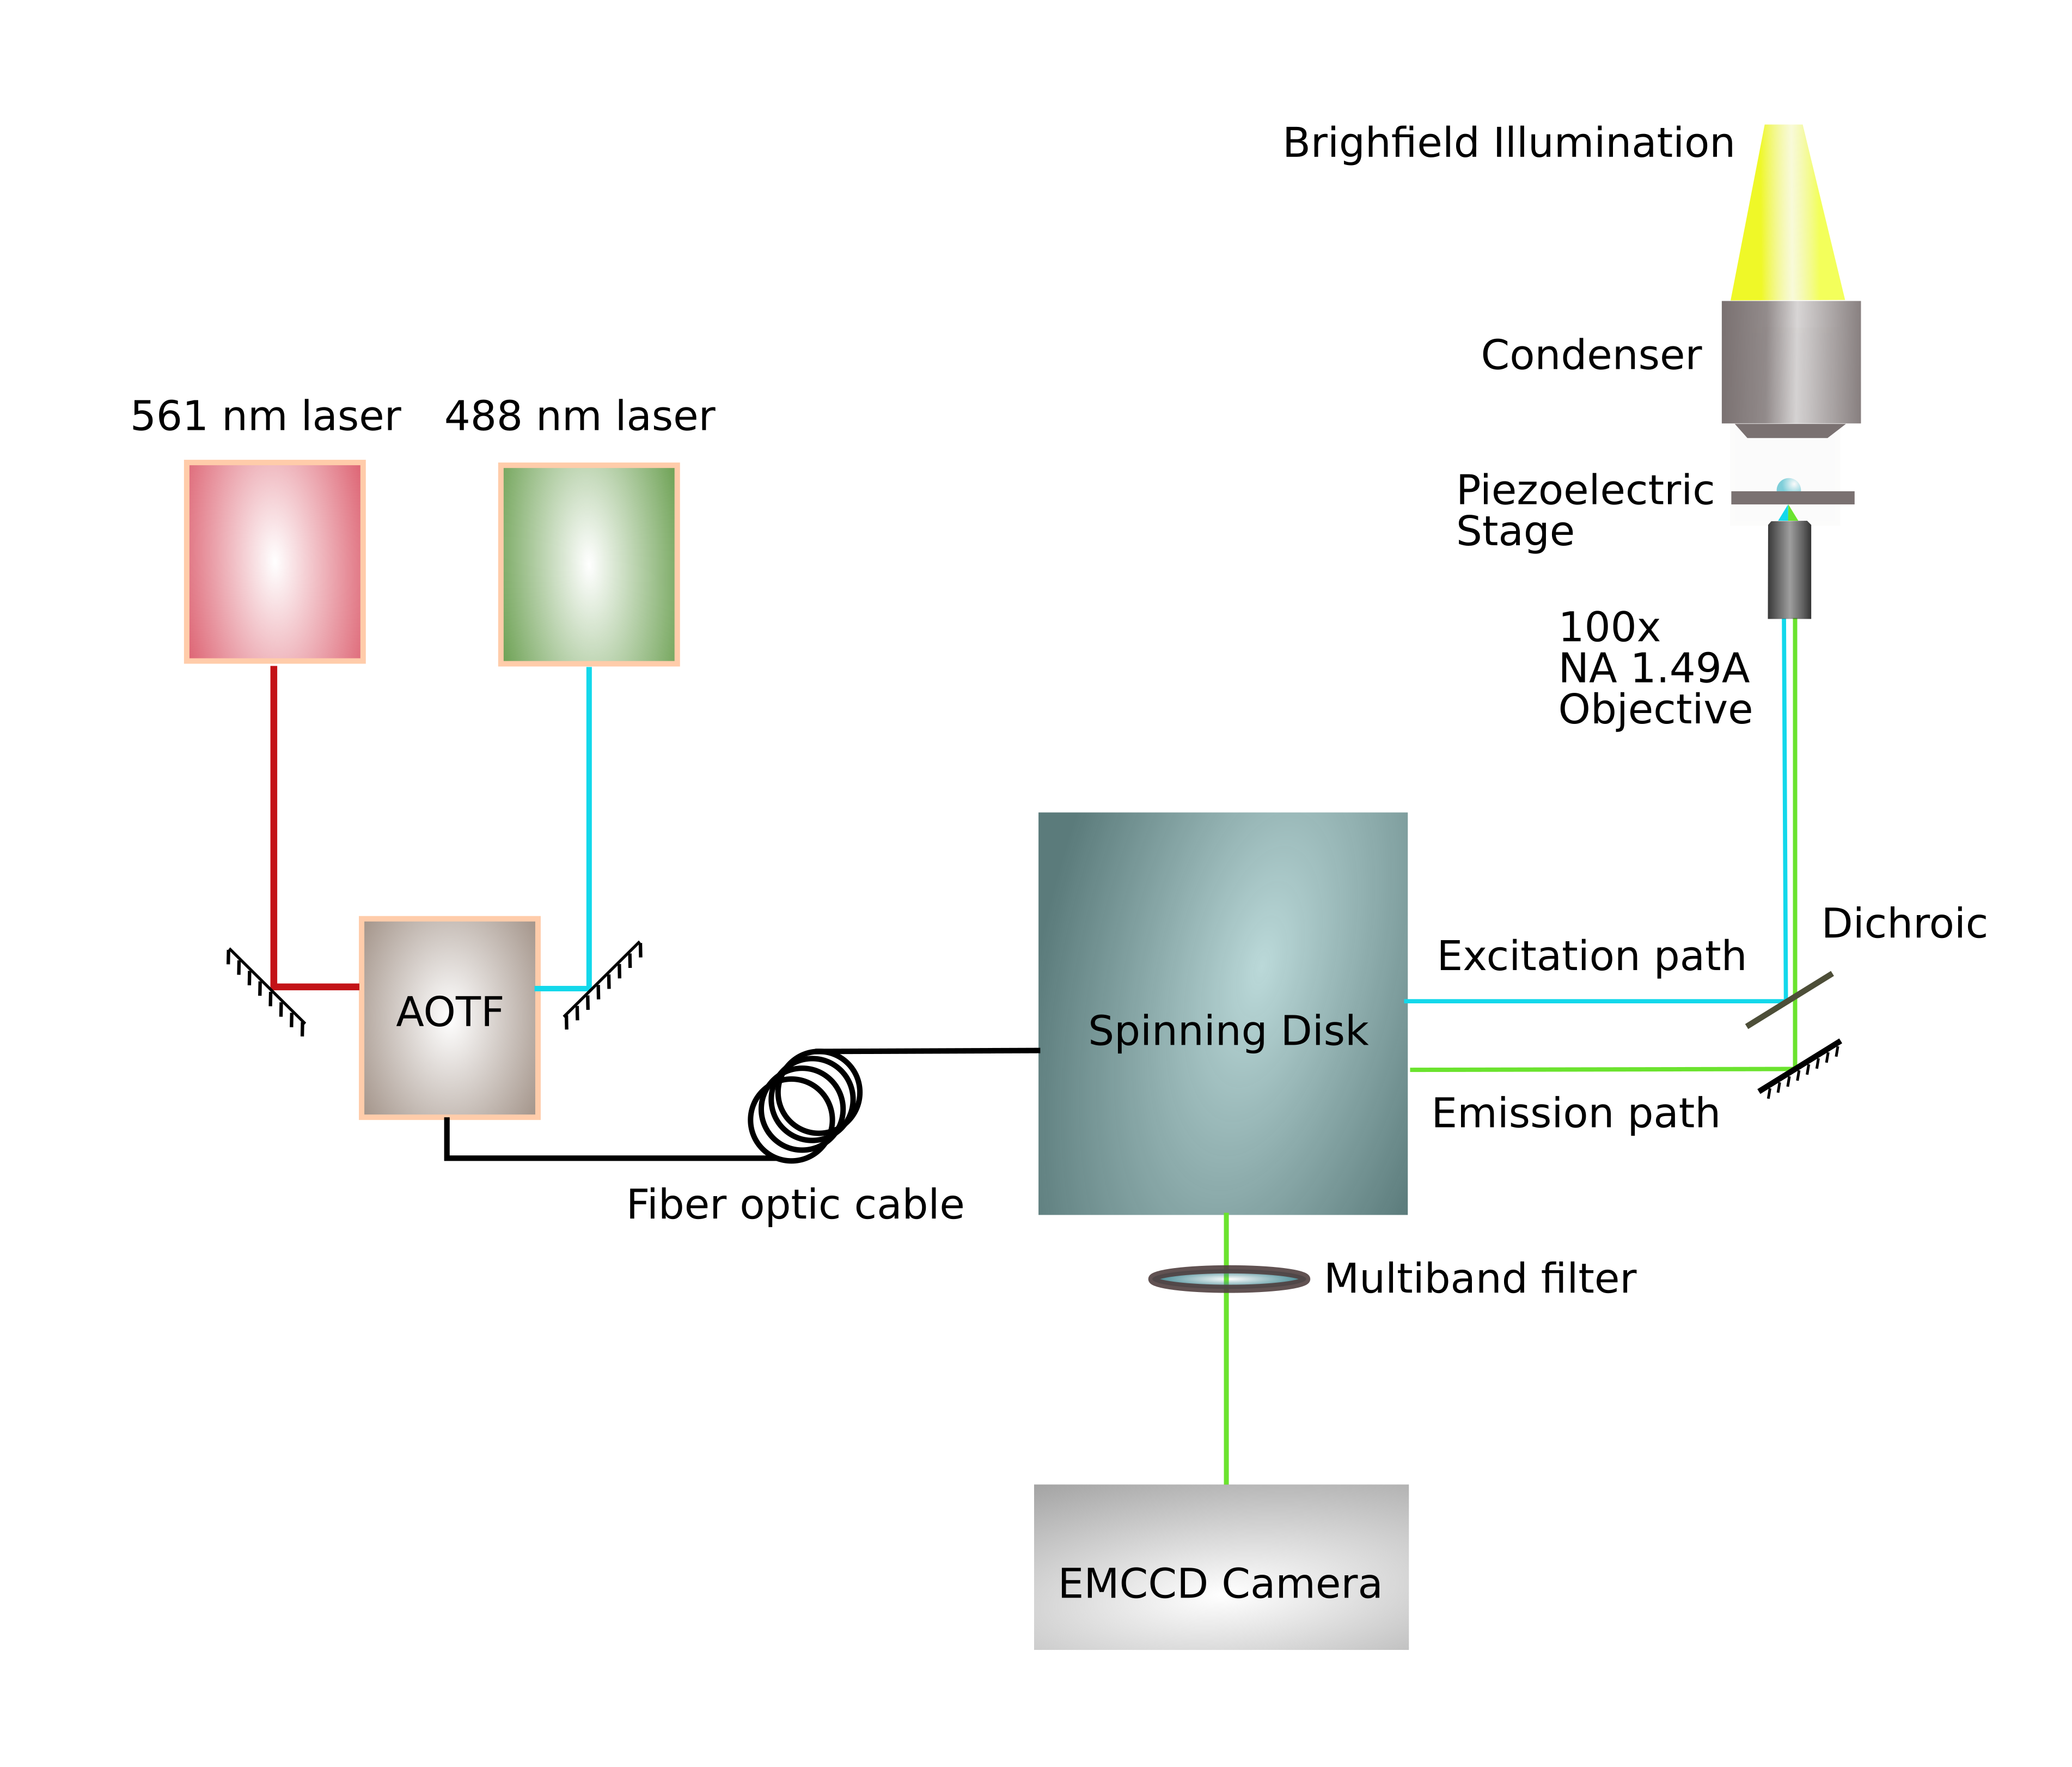
\includegraphics[width=\textwidth]{optics}
    \caption{Schematic diagram of the spinning disk microscope platform.}\label{fig:optics}
\end{figure}
%
\subsection{Strain construction for visualization of matrix structure}\label{sec:strain}
The original cell strain (SMR-12, W303a background stain) expressed the plasmid pVT100U-dsRed (URA), which contained subunit 9 of the F0-ATPase (Su9(1-69)) under the ADH1 promoter with dsRed fused to the C-terminus to constitutively label the mitochondrial matrix. However it was found that the excitation region of the dsRed protein had a significant overlap with the GFP excitation region (\Fref{fig:spectra}).
%
\begin{figure}[htp]
	\centering
    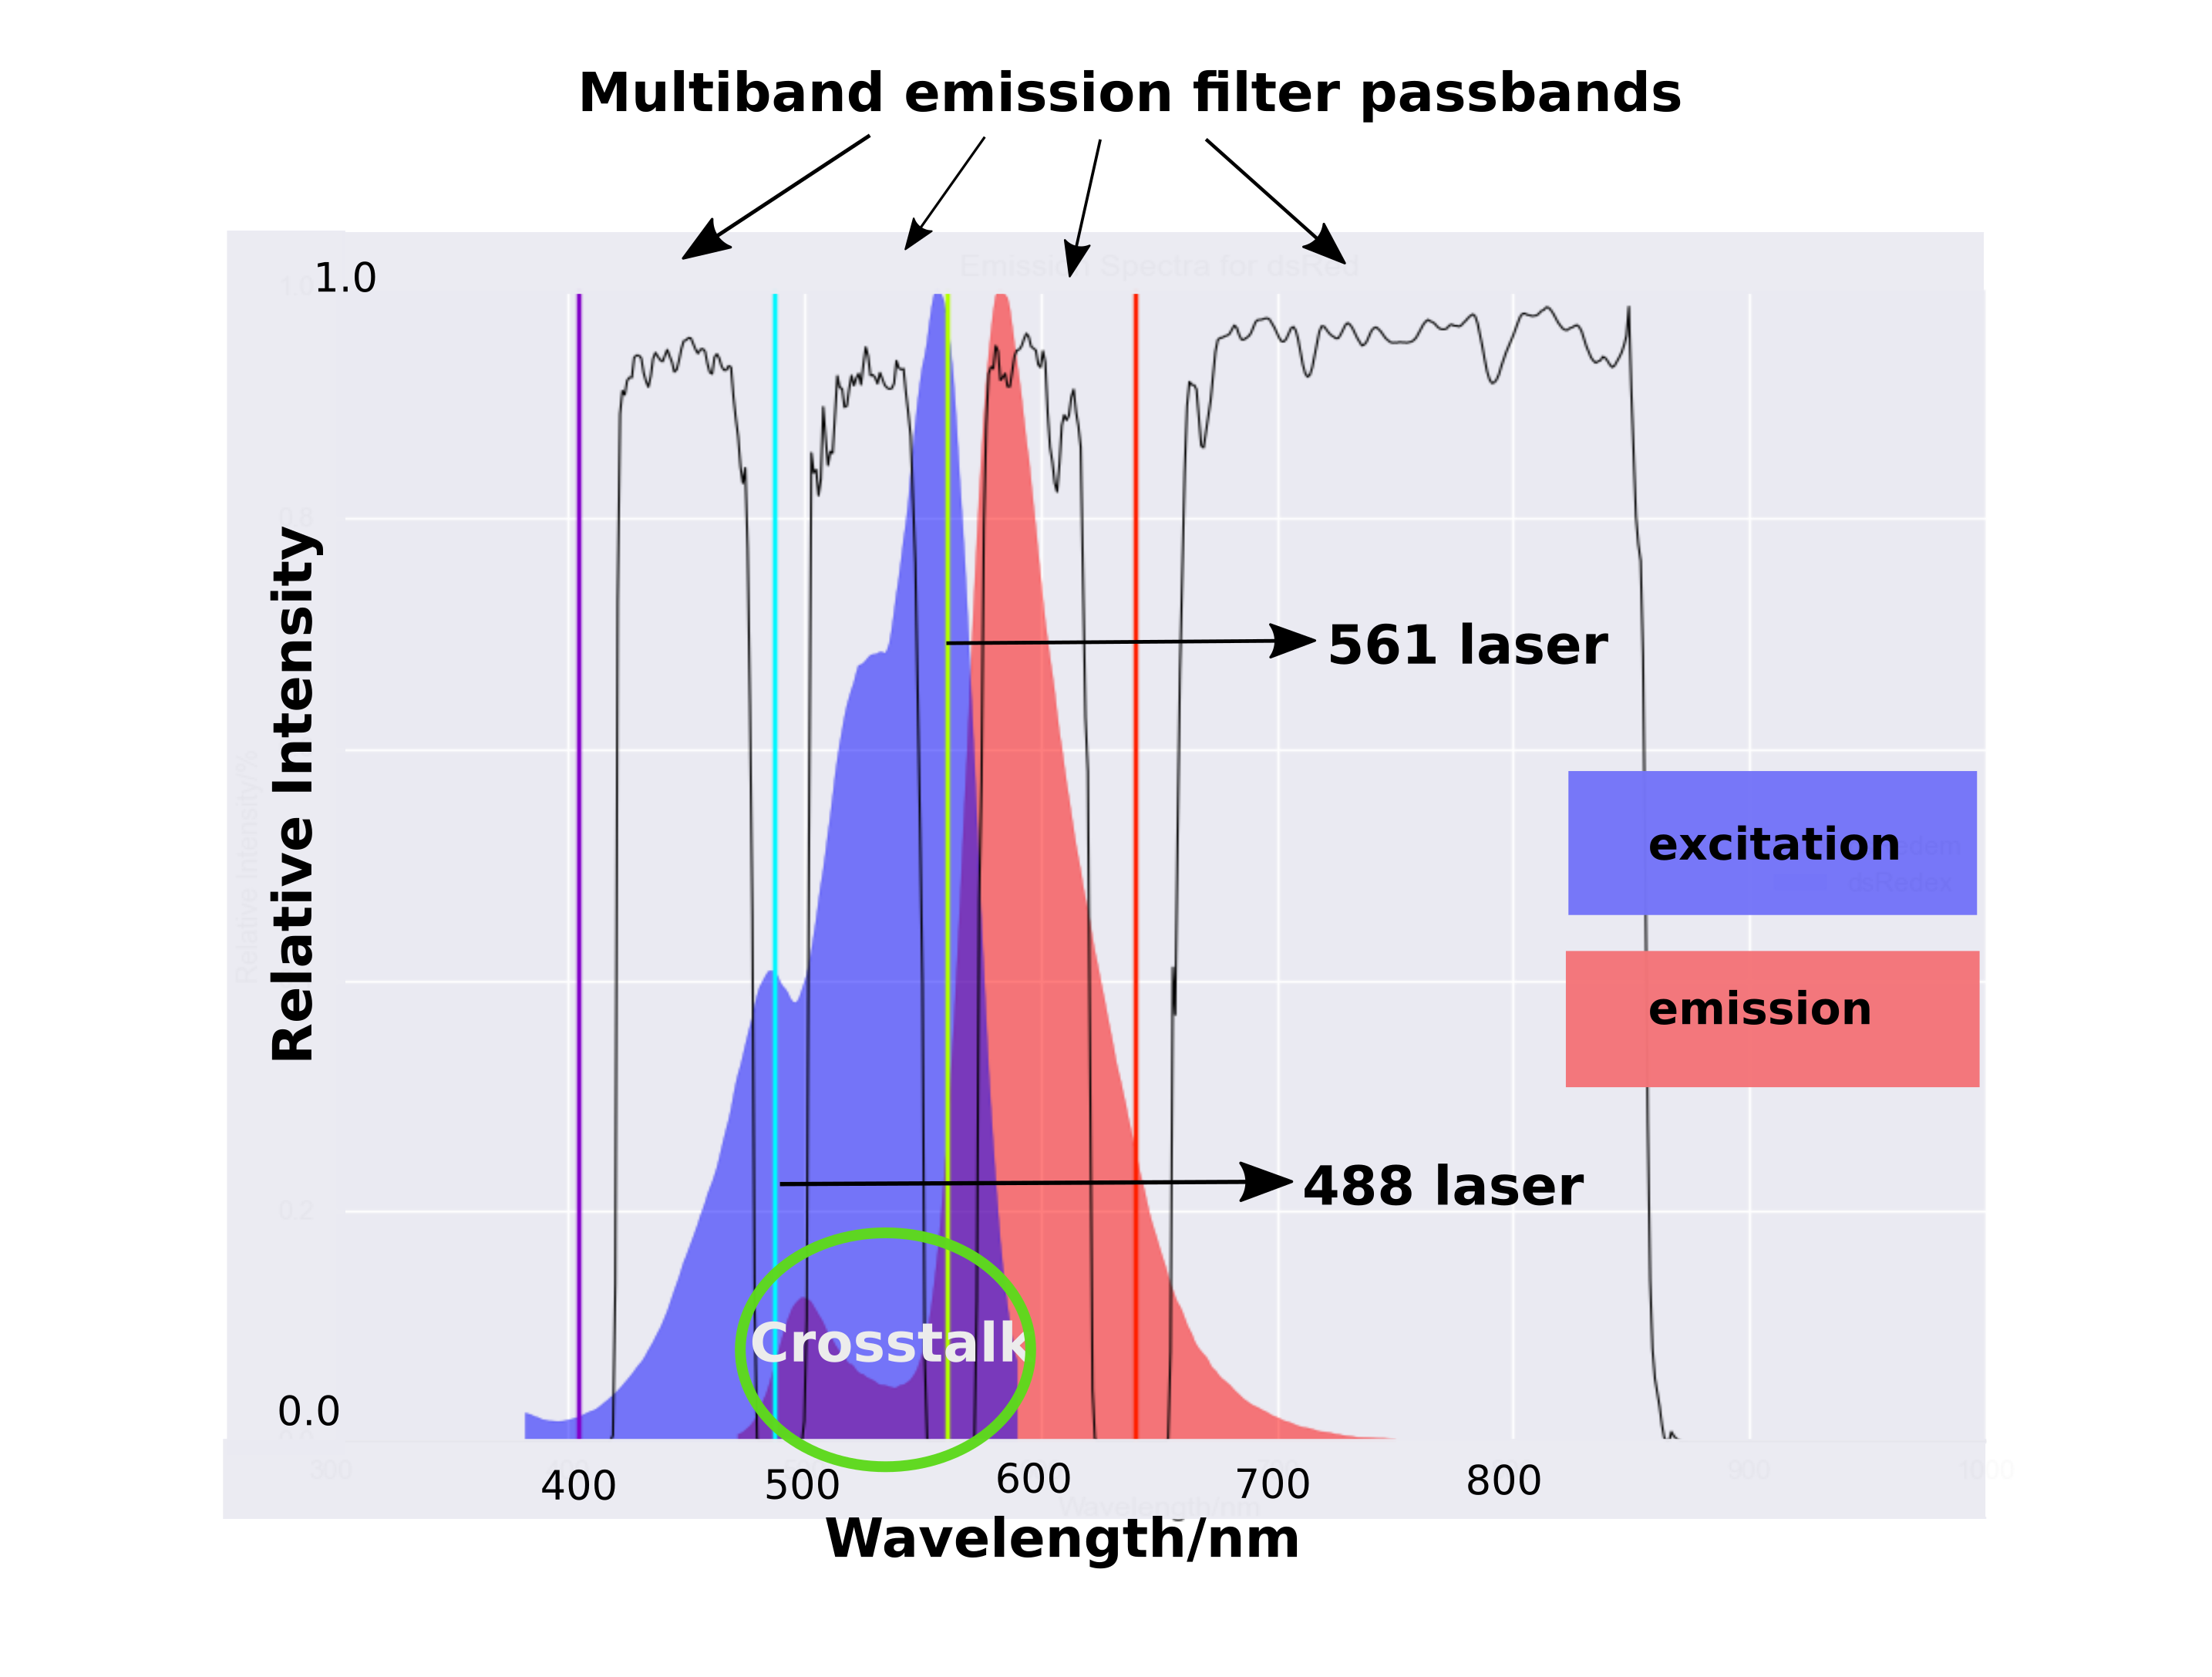
\includegraphics[width=\textwidth]{spectra}
    \caption[Excitation-emission spectra of dsRed mitochondrial matrix marker]{Excitation-emission spectra of dsRed (561nm peak excitation) showing significant region of emission crosstalk from GFP excitation (488nm).}\label{fig:spectra}
\end{figure}
%
This resulted in significant channel crosstalk from the dsRed protein when imaging in the GFP channel (\Fref{fig:xtalk}). To overcome this, the plasmid pFA6a-yomRuby2-Kan (gift of Kurt Thorn, UCSF \cite{lee_improved_2013}) expressing a yeast codon optimized deep red fluorescent protein (mRuby2) was PCR amplified with primer sequences \texttt{\seqsplit{ 5$'$ACAGCGGGTACCATGGTGTCCAAAGGAGAGGAGTTAATC$'$3}} and \texttt{\seqsplit{ 5$'$ACAGCGCTCGAGCCTTACTTATACAATTCATCCATACCACCGC$'$3}} (\Fref{fig:plasA}). The insert was cloned into a matrix targeting plasmid, pVT-100UGFP2 (gift from Jodi Nunnari, UC Davis \cite{meeusen_mitochondrial_2004}), at the XhoI and Kpn restriction sites \Fref{fig:plasB}. Colonies of this new strain (SRY-124, background strain W303a) expressing this new plasmid, pVT100-mRuby2 (URA) were verified by digestion at the EcoRI and HindIII + SphI site (\Fref{fig:plasC}).
%
\begin{figure}[htp]
	\centering
    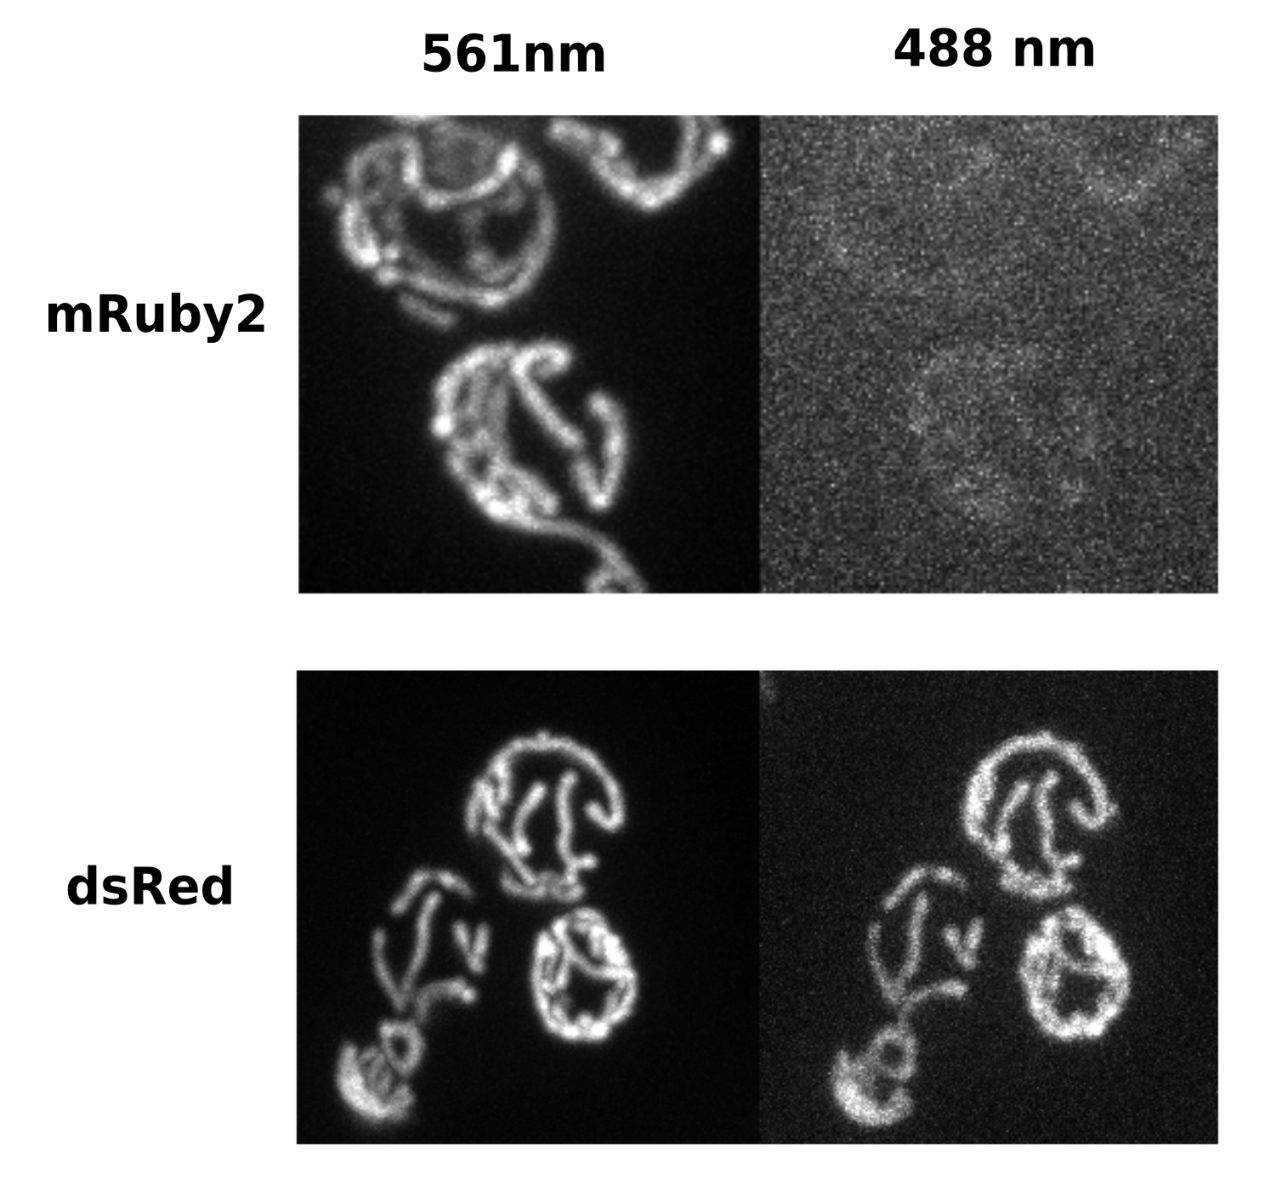
\includegraphics[width=\textwidth]{b4after}
    \caption[Comparison of crosstalk levels in mRuby2 and dsRed.]{Comparison of crosstalk levels in mRuby2 and dsRed.\\
    Shown in this figure are cells expressing either mRuby2 or dsRed and imaged at 561nm and 488nm. The optimum excitation frequency for these proteins are at 561nm, but significant crosstalk is apparent in dsRed when excited at 488nm. Theoretically with zero crosstalk there is zero signal in the 488nm channel, but the intensity of the 488nm channel was 20\% of the value in the 561nm channel. This percentage (and hence crosstalk level) was significantly reduced in mRuby2 (488nm intensity was 3\% of the 561nm channel).}\label{fig:xtalk}
\end{figure}
% 
\begin{figure}[htp]
	\centering
    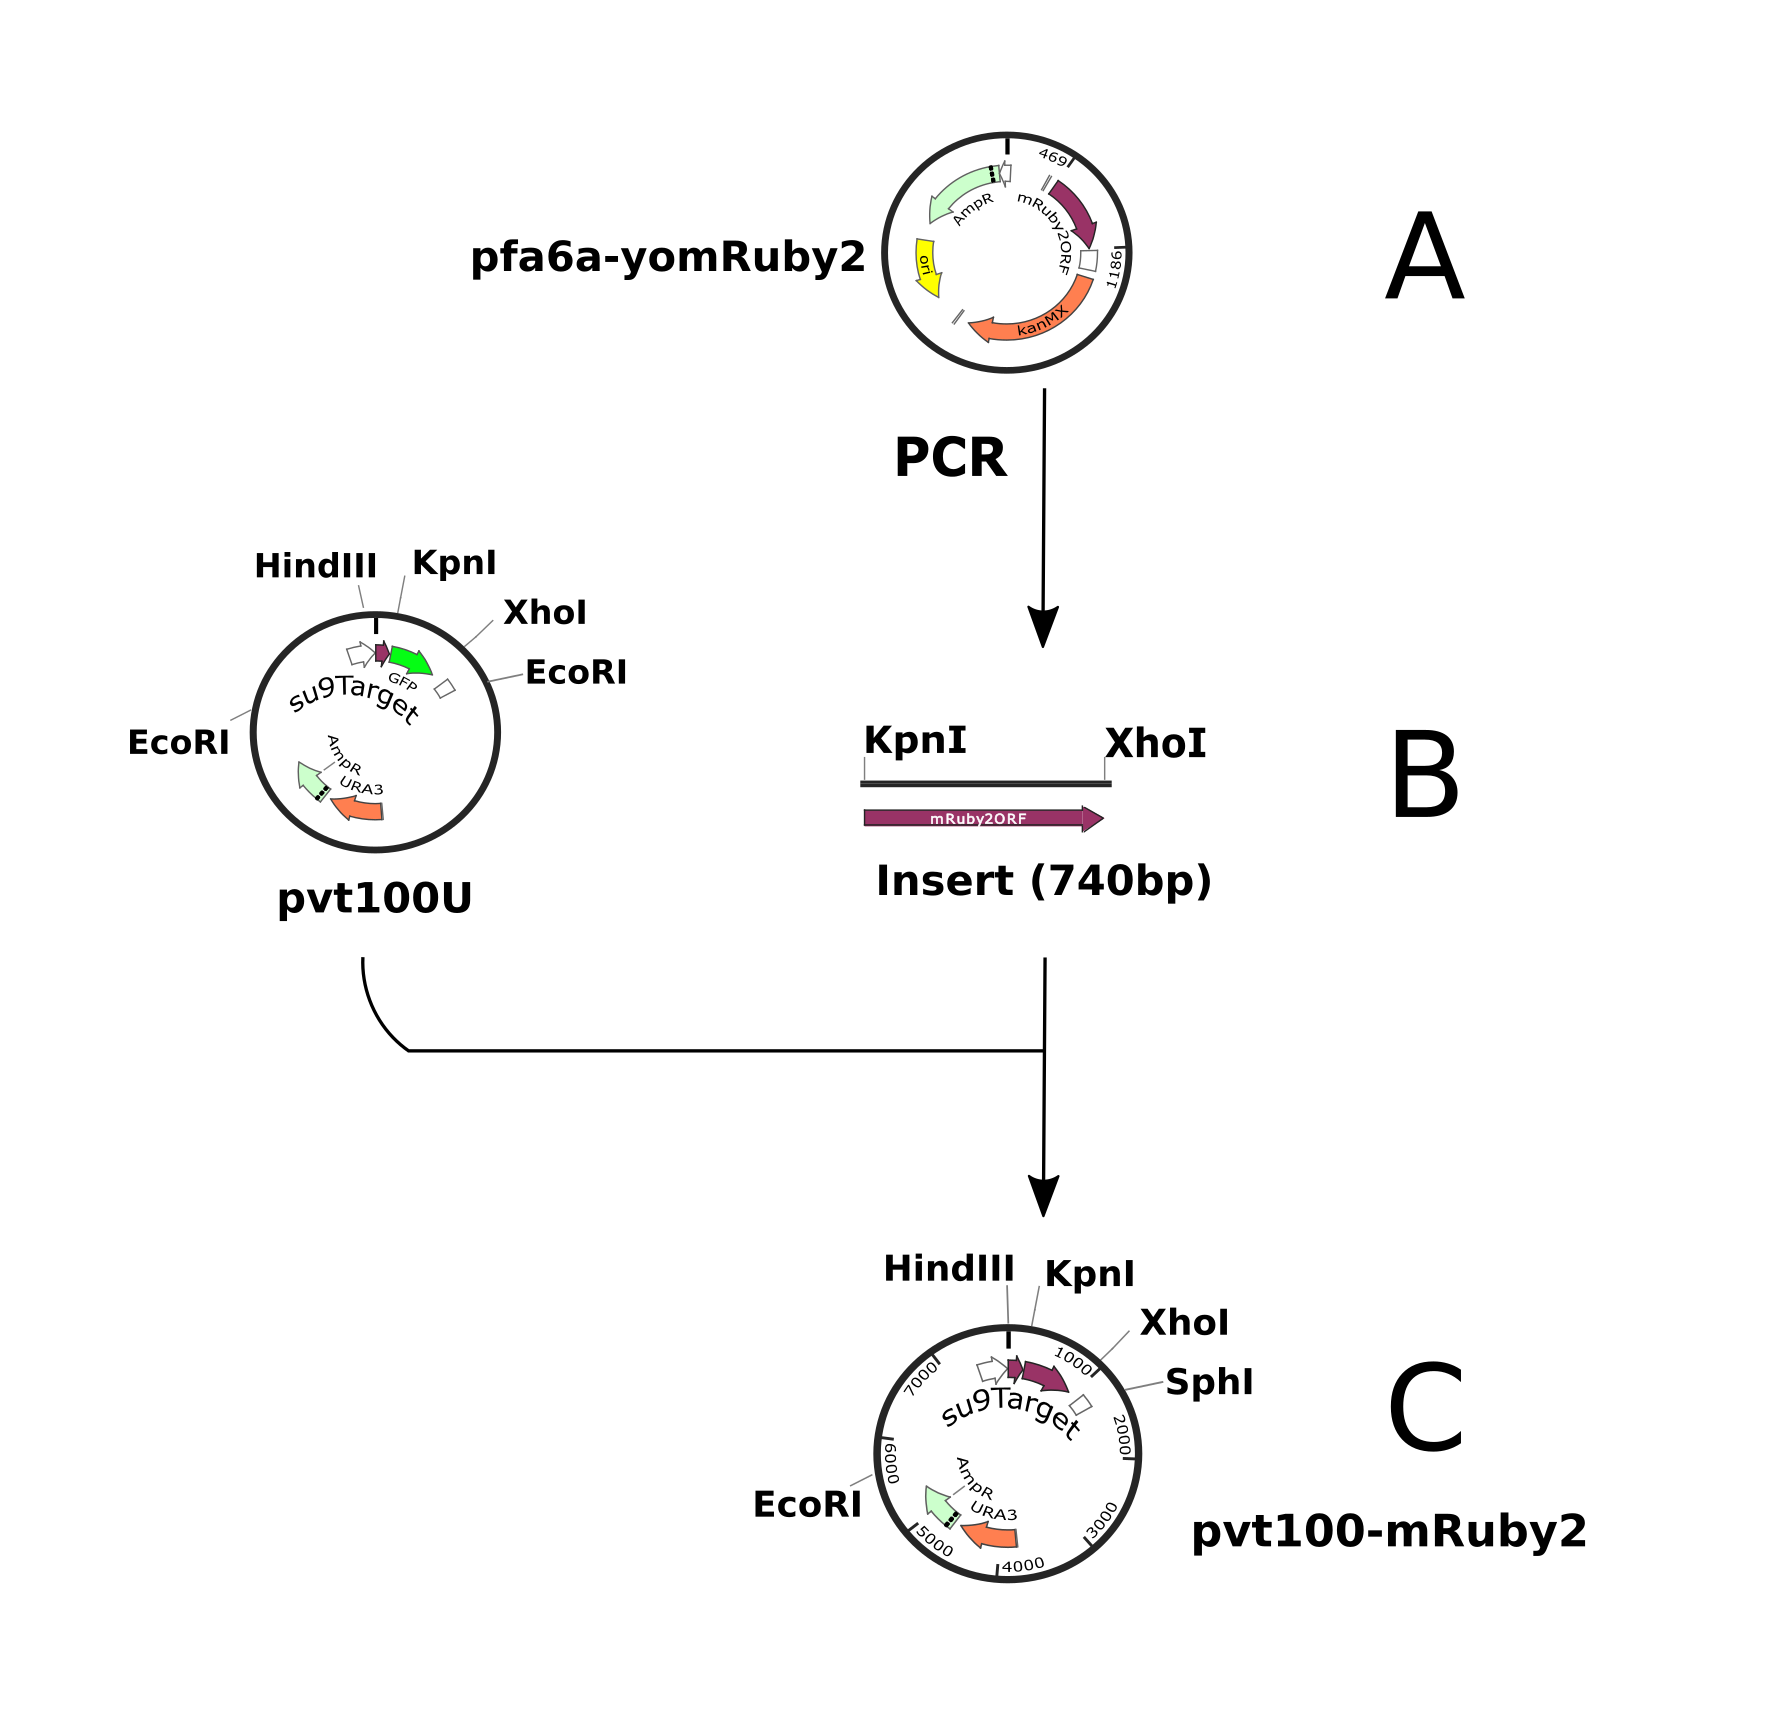
\includegraphics[width=\textwidth]{plasmid}
        \subcaptionbox{Original plasmid (gift of Kurt Thorn, UCSF) containing the mRuby2 sequence.\label{fig:plasA}}[\linewidth]{}
		\subcaptionbox{Insert was generated by PCR amplification of mRuby2 sequence at the KpnI and XhoI restriction sites and cloned into pvt100U-GFP2 (gift of Jody Nunnari, UC Davis).\\Primer sequences for the insert were \texttt{\seqsplit{5$'$ACAGCGGGTACCATGGTGTCCAAAGGAGAGGAGTTAATC$'$3}} and \texttt{\seqsplit{5$'$ACAGCGCTCGAGCCTTACTTATACAATTCATCCATACCACCGC$'$3}}.\label{fig:plasB}}[\linewidth]{}
		\subcaptionbox{The new plasmid, pvt100-mRuby2 (URA) was cloned into W303a background strain and the new strain was SRY-124. The plasmid was verified for correct insertion by digestion at the HindIII and SphI site.\label{fig:plasC}}[\linewidth]{}
		\caption{Plasmid construction details for pvt100-mRuby2 for cloning into SRY-124.\label{fig:plasmid}}
    \end{figure}
%
This new strain exhibited significantly reduced crosstalk from the mRuby2 fluorescent protein when imaging in the GFP region, which is where the functional reporter DiOC$_6$ operates in (\Fref{fig:xtalk}). On average the amount of crosstalk was reduced from an average of about 20\% using dsRed to less than 3\% when using mRuby2.
\subsection{Cell preparation and loading of functional dye}\label{sec:loaddye}
 Cells from strain SRY-124 (described in \fref{sec:strain}) were inoculated from -URA selection plates and cultured overnight at 30°C in a roller drum in the growth media of interest (Yeast Extract + Peptone + either 2\% glucose (YPD), 2\% glycerol+ 2\% ethanol (YPE), 2\% lactate (YPL) or 2\% raffinose (YPR)). A 5 ml 0.05 OD dilution from this overnight culture (which was at \textasciitilde{0.5} OD$_{600}$) was grown to mid-log phase (0.4--0.5 OD$_{600}$). Samples were pipetted out into a 1.5 ml microcentrifuge tube and diluted down in growth media to a ratio of 1:8 before been vortexed briefly to break up cell clumps. 
The cells were stained with DiOC$_6$ (D-273, Thermo Fisher) to a final concentration of \SI{100}{\nmol} from an original master stock concentration of \SI{10}{\umol} (in ethanol). The loaded cells were incubated for 30 minutes at 30°C, spun and wash before reloading in fresh growth media with \SI{100}{\nmol} of DiOC$_6$.

A glass bottom 96 well plate was treated with 1\% Glassclad18 (Gelest Inc, PA) for 5 minutes and oven dried at 70°C overnight. Glassclad18 is a monomeric octadecylsilane glass surface coating that imparts a negative charge to the surface. This ensures that the DiOC$_6$ dye does not bind to the glass, which would result in a high background and reduce the signal to noise ratio from the mitochondria (\Fref{fig:glas18}). Subsequent to surface treatment, each well was loaded with \SI{100}{\ul} of Concanavalin-A (C-5275, Sigma Aldrich) to help cell adhesion to the glass surface. Each well was then loaded with \SI{100}{\ul} of growth media containing cells stained with DiOC$_6$ (D-273, Thermo Fisher) and allowed to incubate at 30°C for about 15 minutes to allow the cells to adhere to the glass surface. The remaining cells in the solution were aspirated and \SI{200}{\ul} of fresh growth media containing \SI{100}{\nmol} of DiOC$_6$ was loaded into the well and immediately imaged.

%
\begin{figure}[htp]
	\centering
    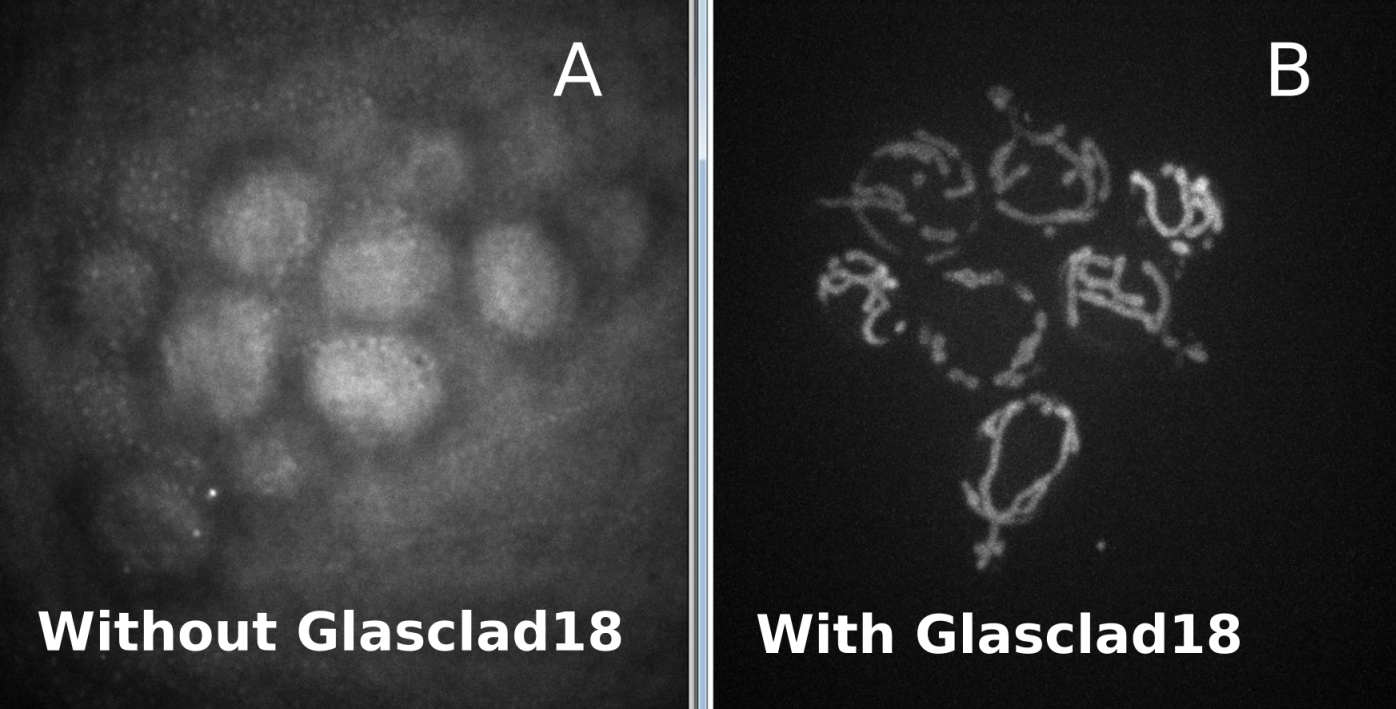
\includegraphics[width=.85\textwidth]{glas18}
    \subcaptionbox{Maximum intensity projection of a cluster of W303a cells stained with DiOC$_6$ loaded in a glass bottom 96 well plate. The dye adheres to the glass surface, causing a significant background image that washes out the signal from mitochondria stained with the dye.\label{fig:glasA}}[\linewidth]{}
    \subcaptionbox{Maximum intensity projection of a cluster of cells loaded on a well treated with Glasclad18. There is significant improvement in the signal to background noise ratio, enabling the mitochondria stained with DiOC$_6$ to be clearly visible.\label{fig:glasB}}[\linewidth]{}
    \caption[Glas18 surface treatment to improve signal to noise ratio]{Signal to noise ratio improvement from DiOC$_6$ channel (mitochondrial membrane potential (ΔΨ) marker) after application of Glasclad18 on imaging surface.}\label{fig:glas18}
\end{figure}
%
\subsection{Image microscopy pipeline}
The cells that were stained and loaded into the 96 well plate in \fref{sec:loaddye} were immediately transferred to the microscope stage holder with the housing chamber set at 30°C. Each well contained cells growing in different carbon types and were imaged as follows:
\begin{enumerate}[label=\arabic*), leftmargin=*, itemindent=0pc]
\item A field of stationary, non clumped cells expressing the fluorescent protein (mRuby2) adequately with healthy mitochondrial morphology was selected via the eyepiece. Individual cells for imaging were then selected via the camera from a region adjacent to this field.
\item Excitation laser power was selected to the minimum needed to give a good signal to background intensity ratio. The minimum signal over background fluorescence was 1.16 (typical background noise \textasciitilde{2000}, minimum signal \textasciitilde{2400}) for accurate skeletonization by MitoGraph v2.0. Photo-damage of the mitochondria was avoided by using low laser power for each channel (typically no more than 20\% of the max range of the laser). Cells with medium to low expression of the protein were selected in order to minimize crosstalk between the signals from the fluorescent protein and the mitochondrial membrane potential dye. This also avoided aberrant mitochondrial morphology due to over expression of the protein in the mitochondria. Typical intensity values for cells were between 3000 – 5000 a.u.
\item A Z-stack was taken of the cells in order to generate a 3D rendering of the mitochondrial network within the cell. The filter settings were set to the appropriate excitation and emission wavelength of the fluorescent protein being expressed. The bottom and top slice positions were set so that the mitochondria was just slightly out of focus at these positions to ensure that the entire mitochondrial network in the cell was imaged.
\item Exposure time was set at 100 ms to reduce photo damage and minimize organelle movement during z-stack image acquisition. Each channel was switched sequentially by the AOTF before moving to the next z-position to minimize organelle movement between channels (\Fref{fig:zstack}). All hardware controls (stage movement in the z-direction during z-stack acquisition and AOTF laser switching) were triggered via TTL which ensured minimum hardware latency.
\end{enumerate}
%
\begin{figure}[htp]
	\centering
    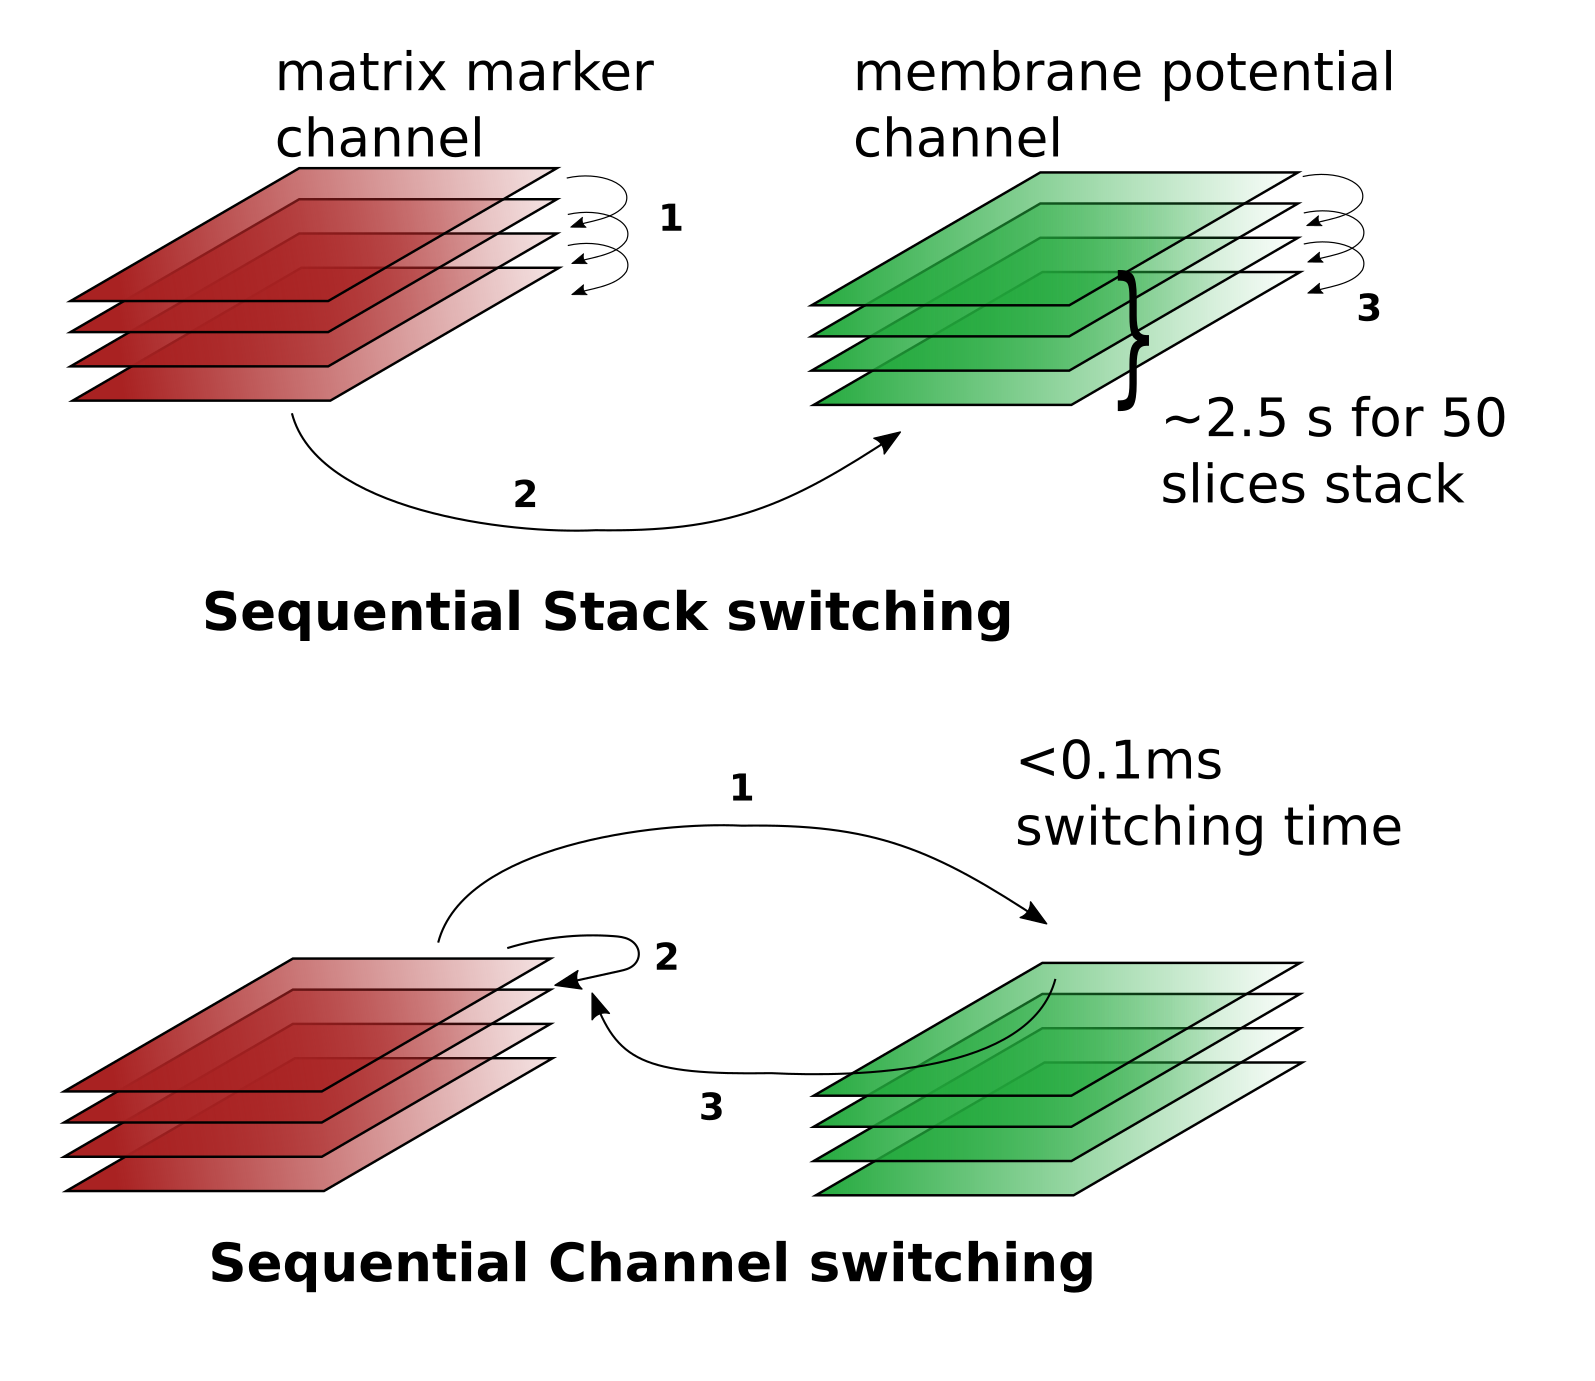
\includegraphics[width=.85\textwidth]{zstack}
    \caption[Comparison of sequential channel vs sequential stack switching scheme.]{Comparison of sequential channel vs sequential stack switching scheme.\\Fast switching time in the sequential channel switching scheme using the AOTF (<0.1ms) ensured that the membrane potential and mitochondrial matrix structural reporting channels (DiOC$_6$ and mRuby2 respectively) were optimally colocalized and did not suffer from organelle movement when compared to the slower sequential stack switching scheme, which typically takes \textasciitilde{2.5} seconds to complete a full stack acquisition.}\label{fig:zstack}
\end{figure}
%
\subsection{Data preparation before input into pipeline}\label{sec:ROI}
Images were saved as 16-bit TIFF stack files. A maximum intensity projection of each Z-stack image was generated automatically via ImageJ batch script. For each cell, the slice with the best focus (defined as where the outlines of the cells in the brightfield stack were least visible) was used to determine if a cell was a budding cell or two individual cells. A region of interest (ROI) was traced out by hand in ImageJ in the corresponding fluorescent image stack (\Fref{fig:budA}). These ROI's were used to crop out the individual cell from the original stack. The cropped out fluorescent channel cell stack was then processed by MitoGraph v2.0 segmentation software. In order to enable cell size measurements, another pair of ROIs were traced (in the brightfield channel) over the mom and bud of the cell and an ellipse fitted to the ROIs (\Fref{fig:budB})
%
\begin{figure}[htp]
	\centering
    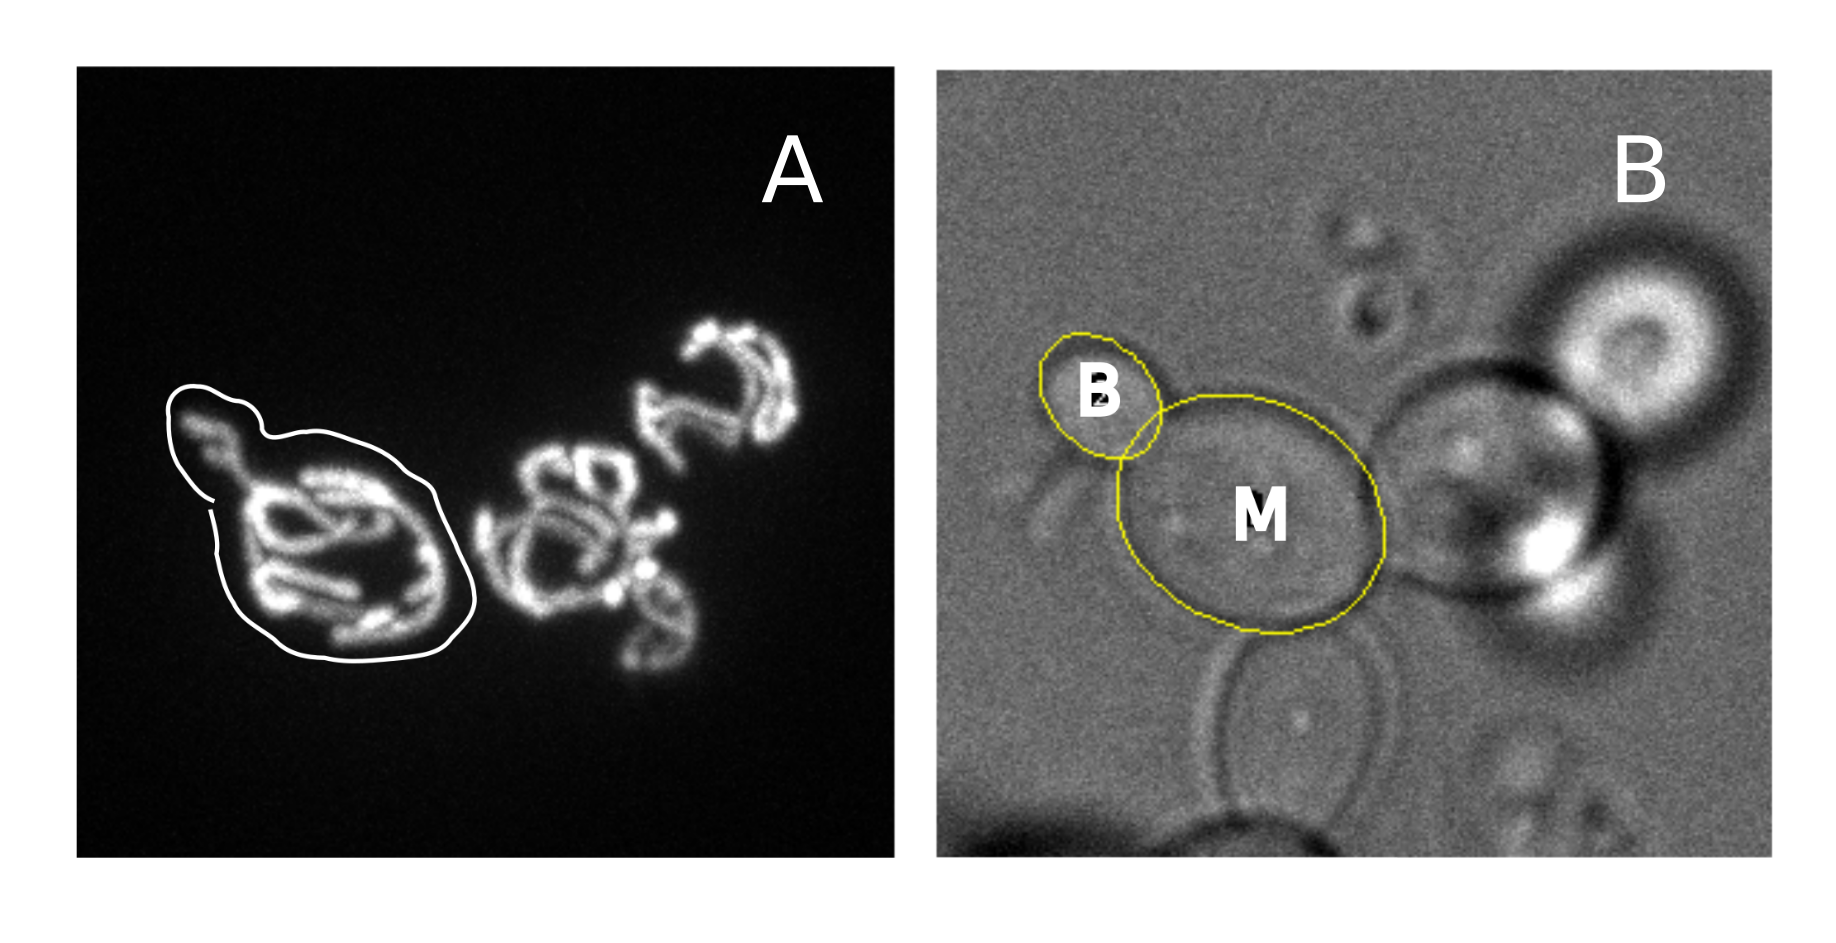
\includegraphics[width=\textwidth]{budtracing}
    \subcaptionbox{Maximum intensity projection of the matrix marker image stack. An ROI (white outline) is hand traced and made into a cropping mask which is applied to the image stack. This cropped image stack was used as input into MitoGraph v2.0 software.\label{fig:budA}}[\linewidth]{}
    \subcaptionbox{Brightfield image of the same cell. In order to enable size measurement of the mom (M) and bud (B) cell, a pair of ROIs were traced and an ellipse fitted over the trace.  \label{fig:budB}}[\linewidth]{}
    \caption{ROI tracing for a budding yeast cell.}\label{fig:budtrace}
\end{figure}
%
\subsection{Artifacts that may arise when mapping ΔΨ to mitochondrial network}\label{sec:artifacts}
 Mapping of ΔΨ to mitochondrial structure is fraught with the potential for artifacts generating a biased or unreliable reading of ΔΨ. These artifacts result from several issues that are related to dye quenching and toxicity, focal plane variation, cell to cell uptake variability and volume variation dependence of fluorescence intensity.
 
While DiOC$_6$ has been long been used as a membrane potential indicator in yeast \cite{hughes_early_2012,john_r._pringle_chapter_1989,koning_dioc6_1993}, most of the other studies mapping function to structure in live mammalian cells tended to use Tetramethylrhodamine (TMRM), the ester form TMRE or the ratiometric dye JC-1. JC-1 is known to have aggregation artifacts and so was avoided. TMRM and TMRE are generally considered less toxic to the respiratory chain compared to DiOC$_6$ and is supposed to have better resistance to self quenching of the fluorophore. However we could not find any discernible impairment of the mitochondria in our hands or in the literature that have also used DiOC$_6$.We found that TMRM could not provide a high enough signal to be successfully mapped to the network, most likely because of the cell wall in yeast that is not present in mammalian cells. Therefore we switched to DiOC$_6$, using the same concentrations, loading protocols and uncoupling tests of other studies that have also used DiOC$_6$ to label ΔΨ \cite{bouillaud_sequence_1994,pena_use_1984,petit_discrimination_1996}. We also verified that at the concentrations we used (\SI{100}{\nmol}), the dye was not operating in quench mode (i.e. could indicate ΔΨ with a higher signal) by observing a higher ΔΨ level in cells that were known to have a high ΔΨ level (respiration) and could be depolarized by an uncoupler (\Fref{fig:fccp}, courtesy of V.Jayashankar).

The intensity of the mitochondrial membrane potential marker and the matrix marker is strongly affected by their position \cite{gerstenberger_heterogeneity_2012,wikstrom_-cell_2007} in the focal plane due to spherical aberration effects that originate from refractive index mismatch. Refractive index mismatch is inevitable when one uses an oil immersion objective to image live cells. This results in a distorted point spread function that causes regions of the cells that are far away from the cover slip to have the lowest signal intensity.

Variation in dye intensity can also result from differences in dye uptake levels between cells. This means that we cannot convert raw intensity values of the ΔΨ channel into absolute voltage to compare ΔΨ between cells, as we cannot control for dye uptake issues that are independent of ΔΨ. This is the disadvantage of using a dye to label ΔΨ, however we can still quantify ΔΨ distributions within a cell as there should be not any variability in dye uptake within the same cell that are not related to ΔΨ.

The last issue relates to intensity variation of the fluorophore due to volume changes. This applies more to the case of the mitochondrial structural marker. Although the expression of the matrix targeted fluorescent protein is not dependent on membrane potential, volume variation along a tubule can result in a thick section of tubule having a higher integrated intensity compared to a thin tubule. 
\subsection{Pipeline to map ΔΨ to mitochondrial network with normalization and scaling to control artifacts}
Having listed all the artifacts that can arise when mapping function to structure, the next step is to account for these artifacts and controlling for their effects where possible when we map function to structure. The first step of the pipeline is a background subtraction of the two channels to correct for camera offset. The background value was set by picking two points without any signal in the original stack. For each channel, a spherical region 2.5 pixels in radius (equivalent to \SI{138}{\nm}) was set along every point coordinate ($x_i,y_i,z_i$) of the skeleton generated by MitoGraph v2.0. A point cloud from this sphere was mapped onto the 3D voxels file of each channel. A mean value of all the points lying within this point cloud was assigned to the point ($x_i,y_i,z_i$).  This averaging served as a smoothing filter to correct for noise/jitter in the channel while reasonably capturing the signals from a typical mitochondrial tubule with thickness \textasciitilde{\SI{300}{\nm}} \cite{egner_fast_2002}.

For the mitochondrial matrix marker, the values were then normalized to 0 and 1 by scaling to the min and max of the channel in that particular cell. This means that the matrix channel was scaled to the intensity of the narrowest portion of the tubule in that cell's mitochondrial network. This controls for the matrix intensity variation due to tubule thickness variations, hence addressing the problem of volume variation dependence of fluorescent protein intensity.

The background subtracted DiOC$_6$ channel representing membrane potential was then normalized to the matrix channel (scaled to min-max). This normalization controls for the focal plane variation problem as both channels are affected similarly by spherical aberration, thus their ratios 'cancel' out the errors. The resulting channel represents a spatial 'heat map' of mitochondrial membrane potential over the mitochondrial network within that cell. A flowchart of the pipeline is shown (\Fref{fig:pipeline})

The source codes for the pipeline modules are included in Appendix \ref{pipecode}.
%
\begin{figure}
	\centering
    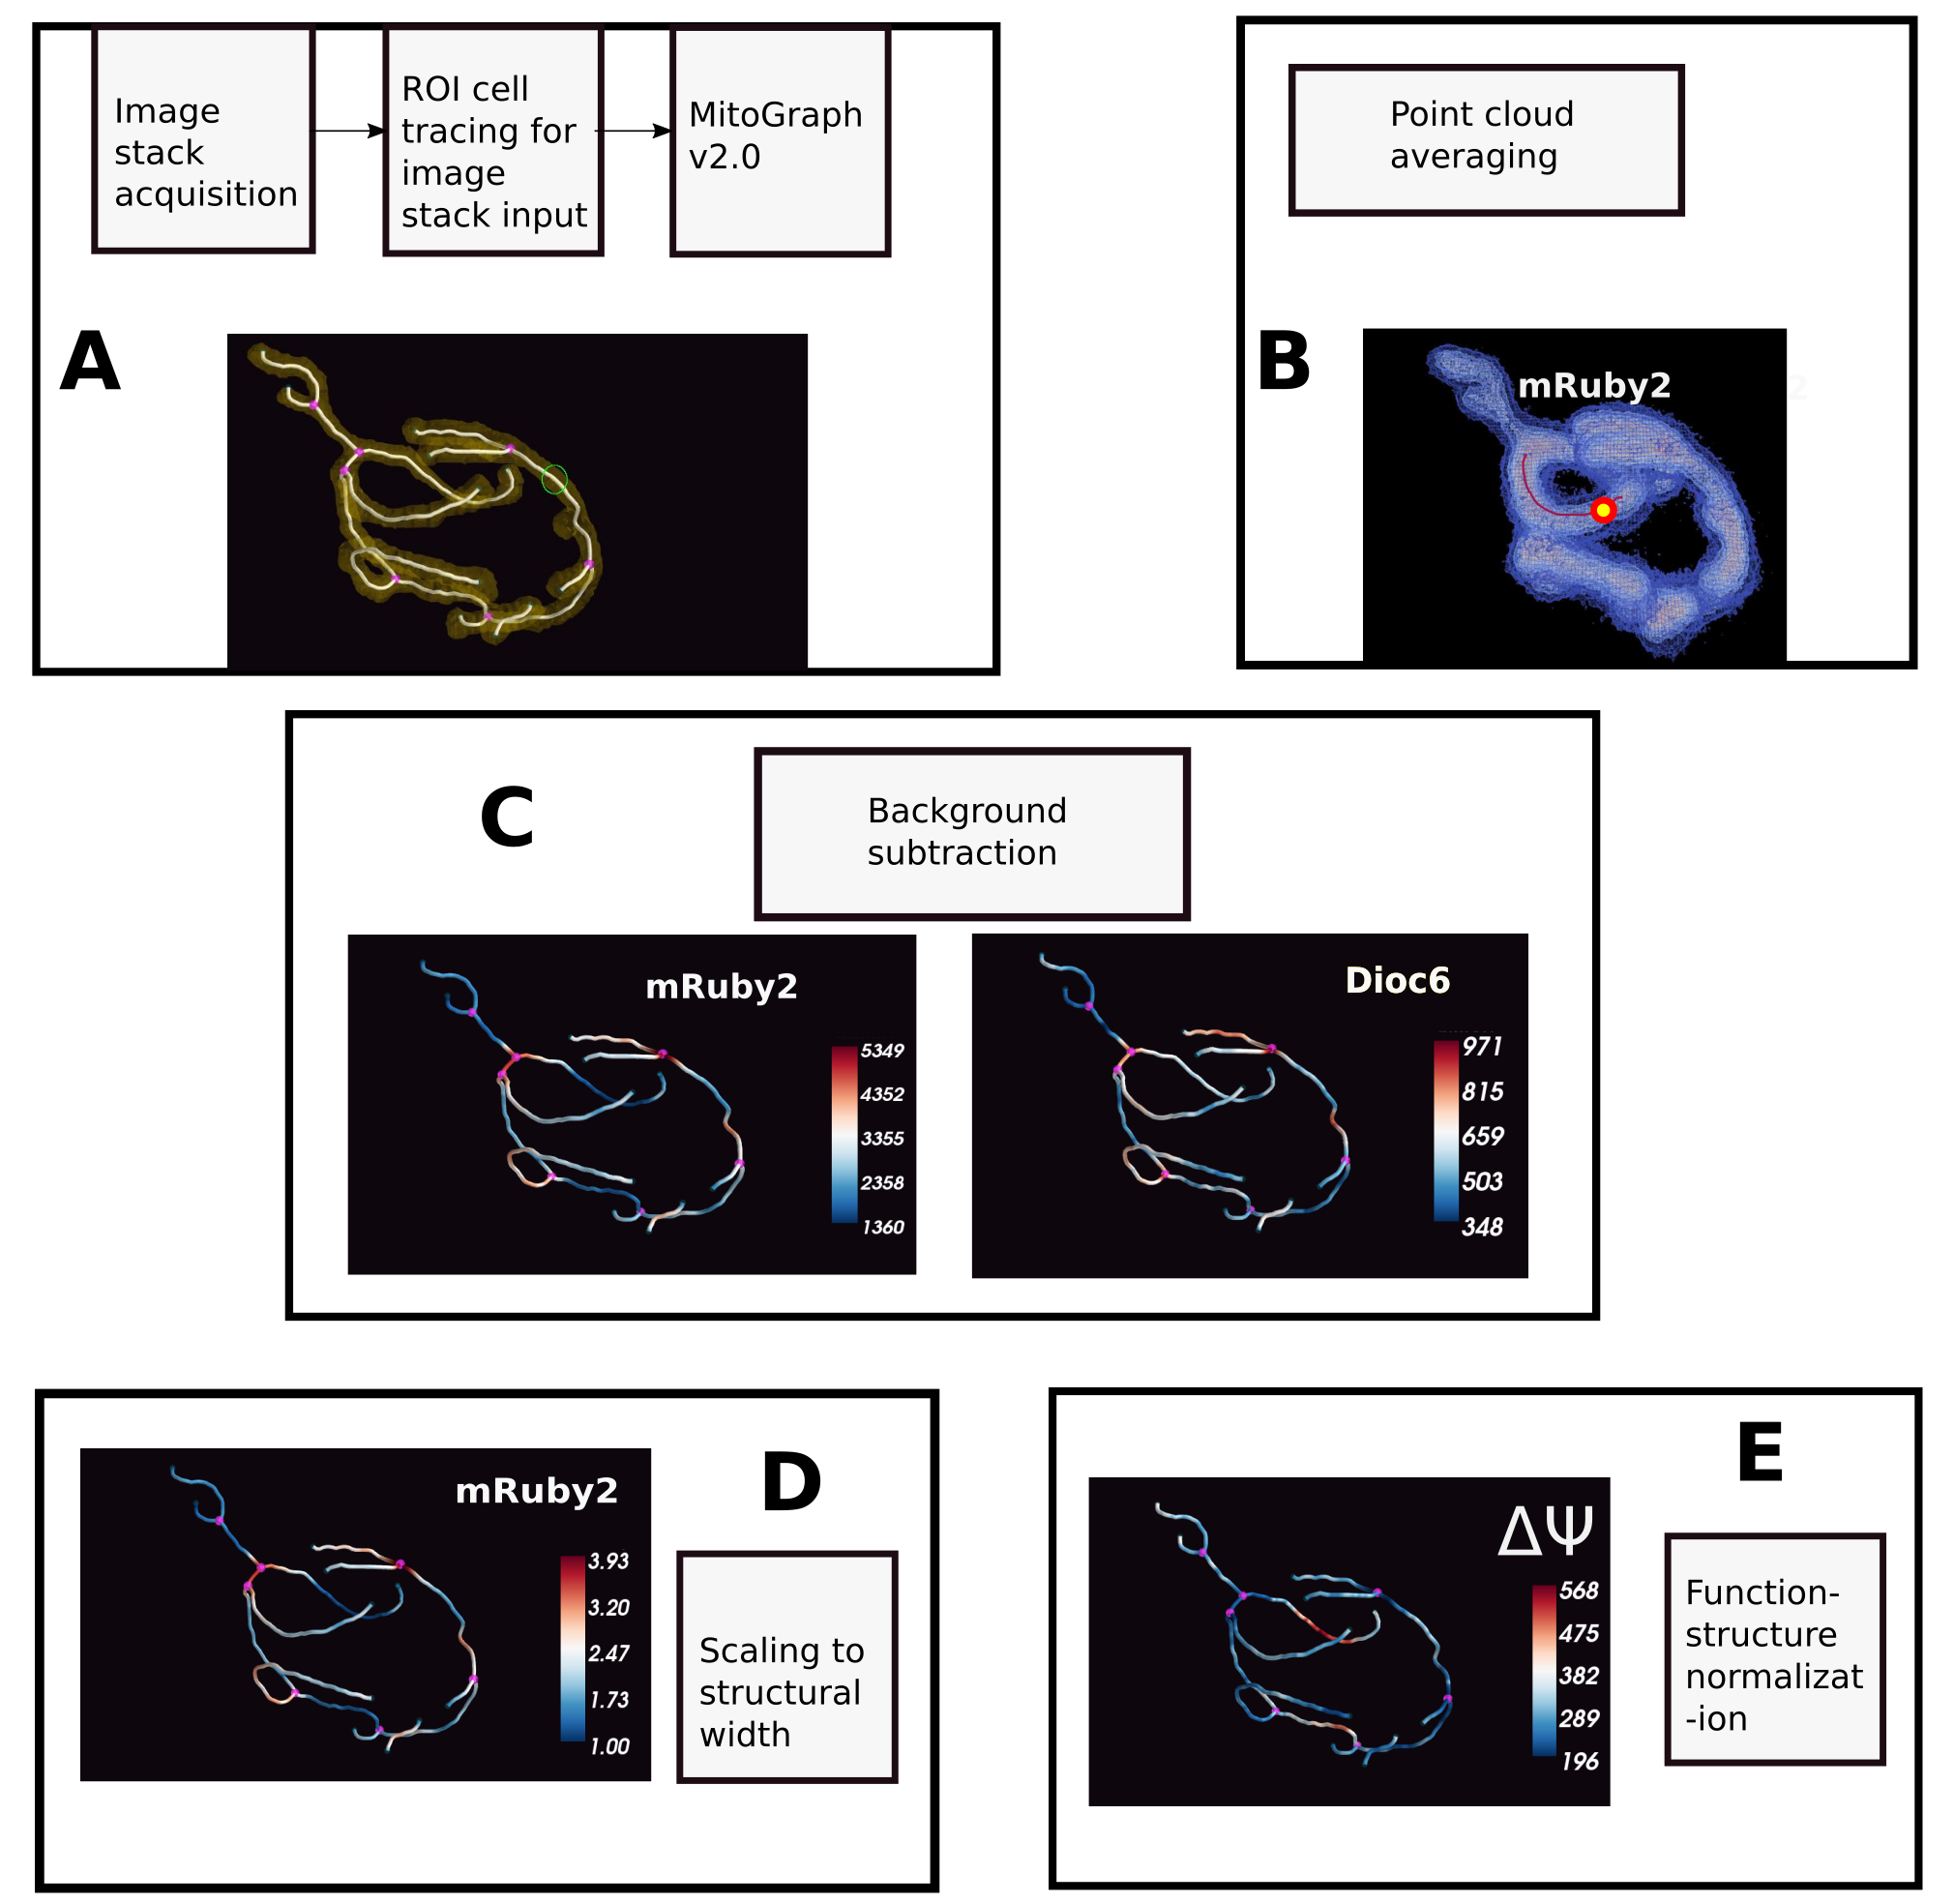
\includegraphics[width=\textwidth]{pipeline}
    \captionof{figure}[Structure-function mapping pipeline]{Pipeline modules for mapping function (ΔΨ) onto structure.\\The boxes A-E roughly correspond to the individual program modules used in the pipeline. Module A represents all steps from image acquisition up to skeletonization by MitoGraph v2.0 to generate a raw skeleton and surface rendering of the matrix marker channel (mRuby2). Module B represents the point cloud averaging from the voxels of the 3D image stack. For each point along the line, the mean intensity value of all points within the red sphere was assigned to the point marked in yellow. Module C represents a background subtraction module that is applied to both matrix marker and ΔΨ channel. The images shown are the skeleton after background subtraction and point cloud averaging for matrix (mRuby2) and ΔΨ (DiOC$_6$). Module D represents a min-max scaling of the pixel intensities to the minimum intensity to control for volume dependence of matrix marker channel due to tubule width variation. Module E represents the spatial heat map of ΔΨ along the skeleton after normalizing the background corrected ΔΨ channel (from module C, DiOC$_6$) with the scaled, background subtracted matrix channel (from module D).}\label{fig:pipeline}
\end{figure}
%
\subsection{Data wrangling – database structure}\label{sec:database}
The raw outputs of MitoGraph v2.0 that are used in the pipeline are a set of coordinates representing a skeleton of the mitochondrial network along with a connectivity list with information on how the points connect to each other. The other outputs that are used are the 16-bit scalar intensity values of each channel for the matrix marker, ΔΨ and tubule width of the mitochondrial network.

The native file format of the data is in the Visualization Toolkit (VTK, \url{http://www.vtk.org/}) format which is a C++ library for 3D scientific visualization with interfaces for Python and other interpreted languages. The native data is 'wrangled' or organized into a standard tidy data form \cite{wickham_tidy_2014} and stored using a database structure with the Pandas data analysis module (\url{http://pandas.pydata.org/}) in Python 2.7. Data wrangling involves reshaping the raw data format structure (i.e. a mitochondrial network) into a form that is most convenient for performing calculations at a scale that is relevant to the type of analysis. The output can then be aggregated if necessary for further calculations downstream or for visual data presentation.

The database (\Fref{fig:database}) incorporates \textasciitilde{100} variables which are measures related to structure and function across multiple size scales as well as measures that relate to either heterogeneity, function or cell asymmetry. These variables were calculated from the outputs of MitoGraph v2.0 as well as other meta-data (for example cell name, cell carbon source) and non MitoGraph v2.0 derived data (such as oxygen consumption rates). The database enables convenient data exploration and multi-scale analysis of structure-function in mitochondrial networks, with the data organized in 'tidy-data' form \cite{wickham_practical_2008} and allowing a layered grammar of graphics presentation of the results \cite{wilkinson_grammar_2005}. A list of variables from the database is included in the Appendix section (\Fref{tab:long}).

The source code for constructing the database is included in Appendix \ref{dbcode}.
\begin{figure}[htp]
	\centering
    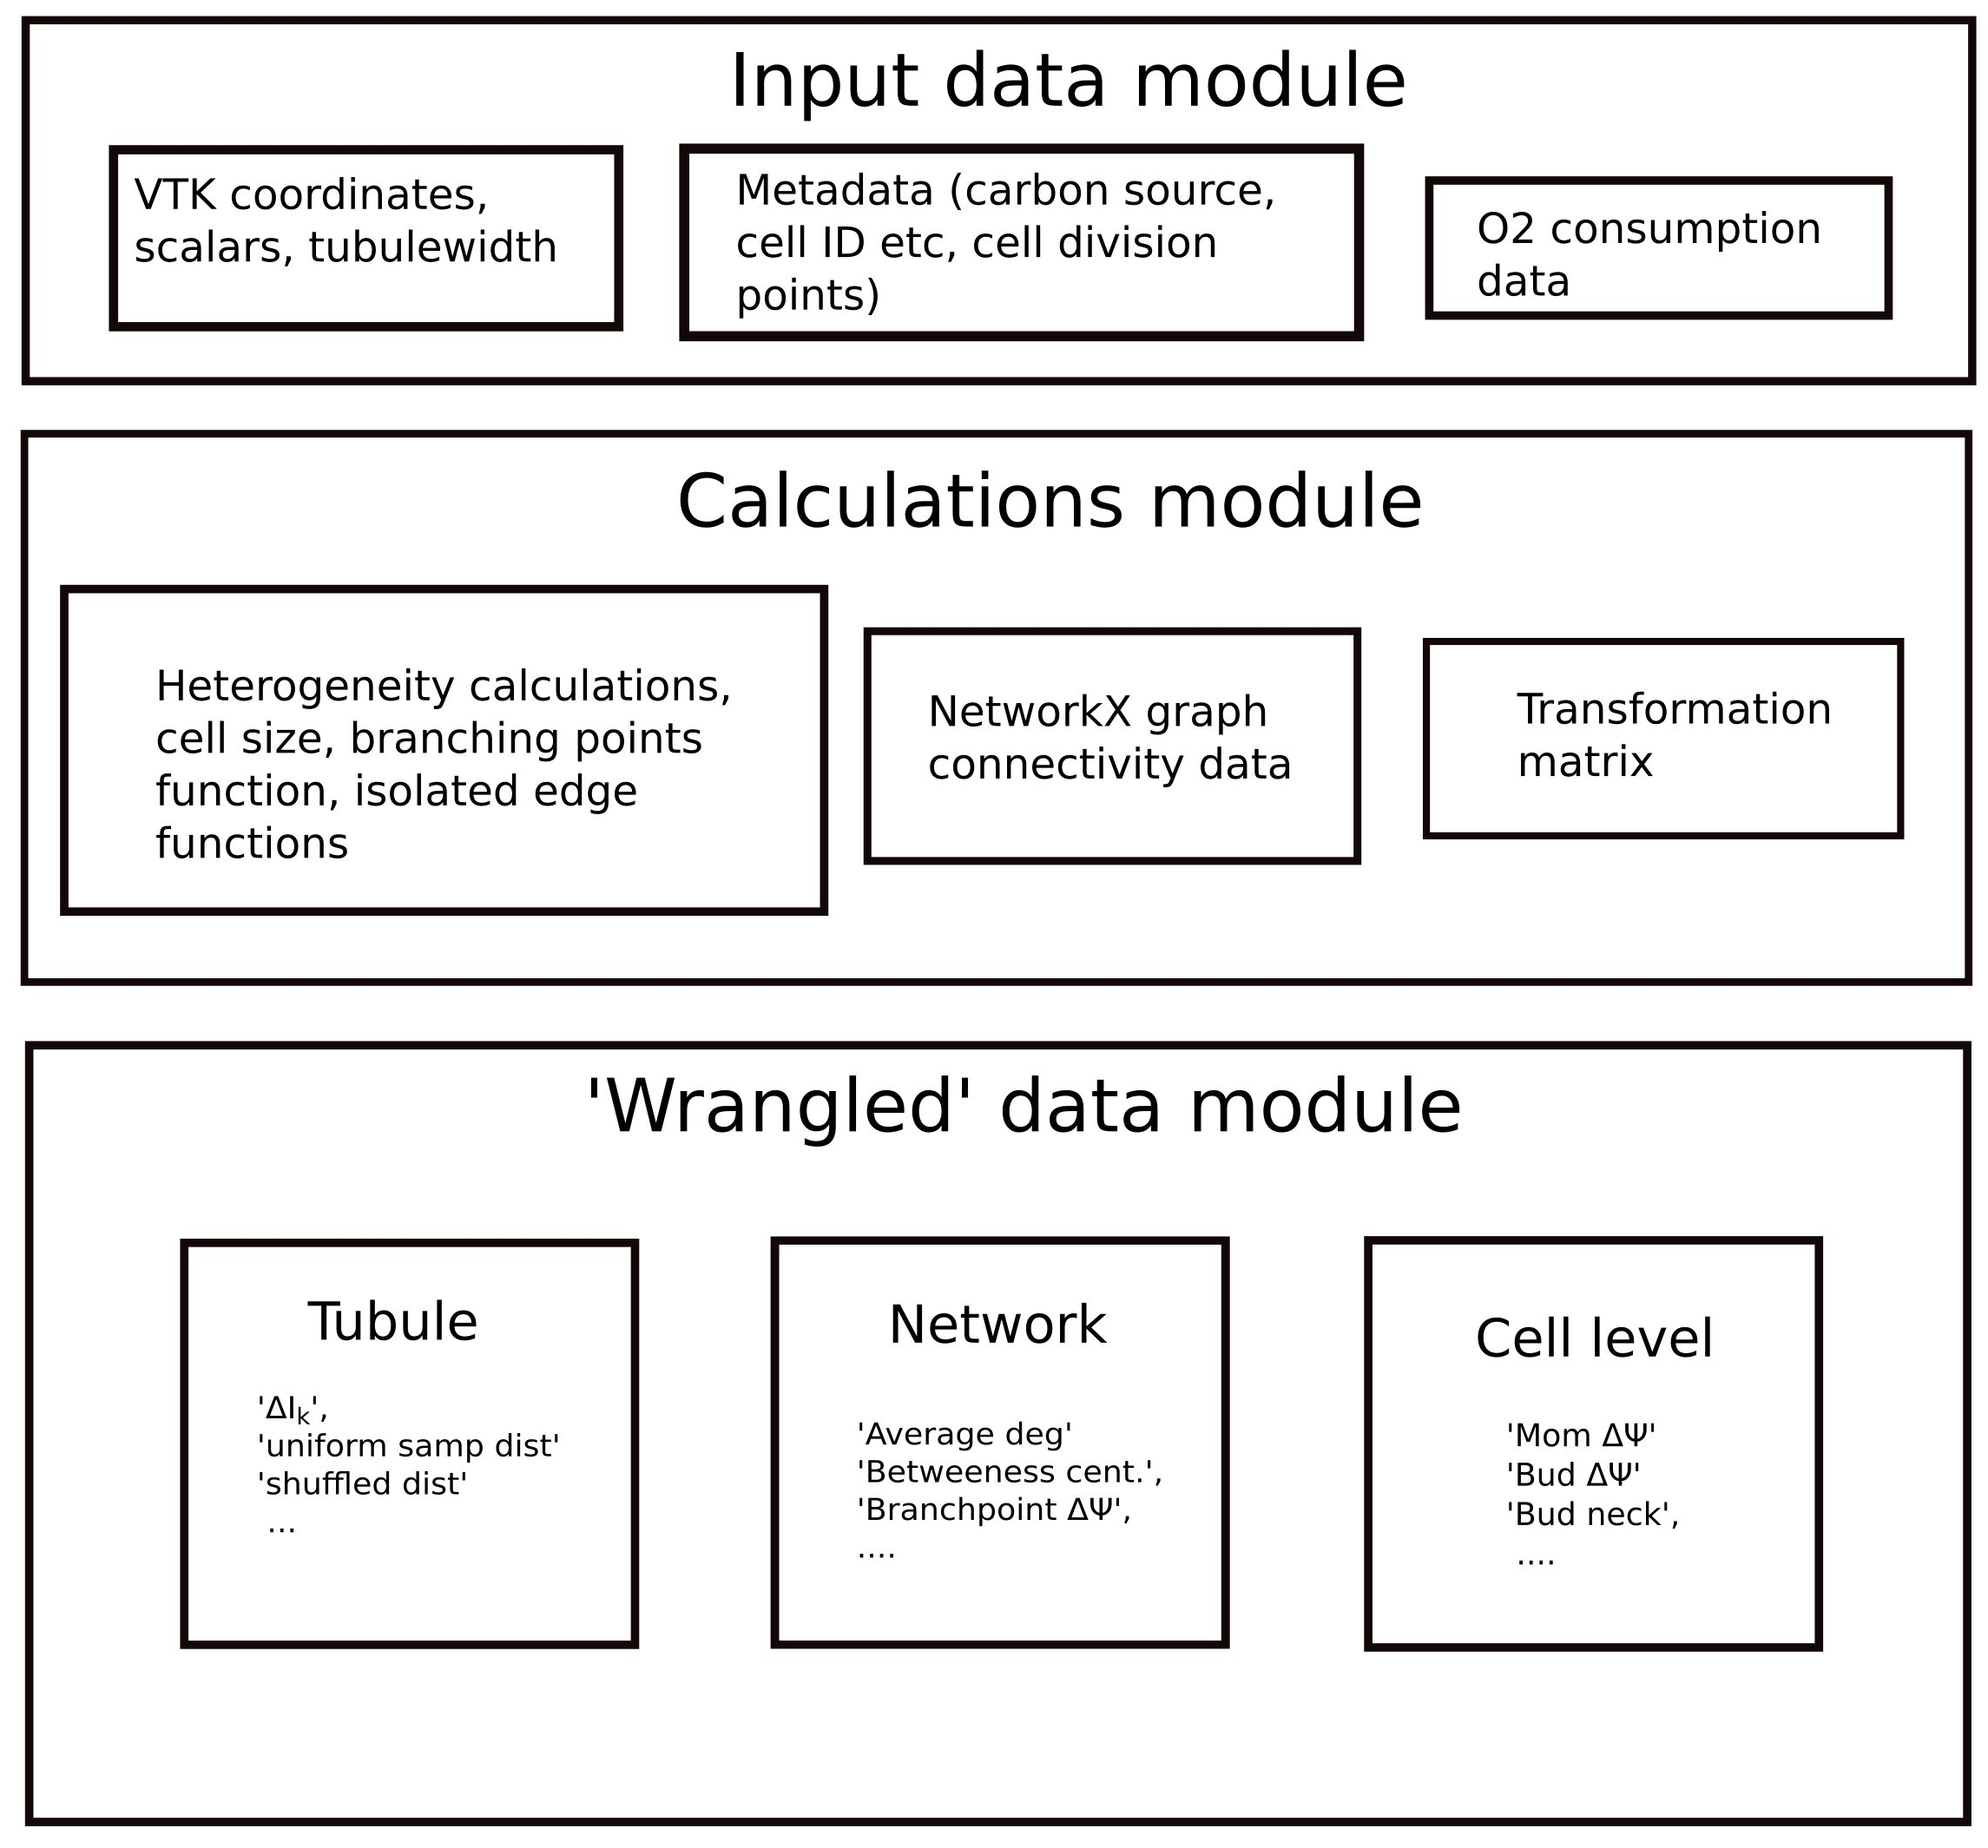
\includegraphics[width=\textwidth]{database}
    \caption[Multi-scale structure-function database]{Schema of database used for multi-scale analysis of structure-function relationship in yeast mitochondrial networks.\\
Shown here is the database used in this thesis which uses the Pandas data analysis module in Python 2.7. The database consists of an input data module, a calculations module and a wrangled data module.
The input data module stores the outputs of MitoGraph v2.0, metadata sources and oxygen consumption data. The primary calculations module processes the data from the input data module to obtain measures such as connectivity, heterogeneity measures and transformation matrix used for calculating mother-daughter cell axis. The processed data is then reshaped and aggregated ('wrangled') into the form most appropriate for the scale and functional measure it will be used for, for example in mother-bud functional asymmetry analysis.}\label{fig:database}
\end{figure}
\chapter[Modulating metabolic state]{ Carbon substrate dependent variation of metabolic state in budding yeast}\label{ch:three}
\clearpage
\section{Introduction}
Budding yeast are able to generate their energy from either fermentation or respiration. When grown in conditions where they are forced to undergo respiration, their mitochondrial networks display an increase in size and appear more connected ('degree of ramification', \cite{jakobs_spatial_2003}). This simple but powerful connection between metabolic state and morphology of the organelle underlies our rationale for varying growth substrates to study the structure-function relationship in yeast mitochondrial networks. We begin this chapter with an overview of how yeast metabolize different carbon substrates using either fermentation or respiration dependent pathways, how cellular respiration and oxidative phosphorylation (OXPHOS) respond to bioenergetic needs of the cell, how we might measure the bioenergetic state of cells and what the expected levels of these measurements would be for the substrates we used in this study.

The preferred sugar sources of budding yeast are glucose and fructose \cite{bergman_growth_2001}. When glucose levels are high, the expression of enzymes and proteins needed for metabolizing other types of carbon sources and mitochondrial biogenesis are repressed and all energy is derived via fermentation. This phenomenon is known as carbon catabolite repression or alternatively glucose repression \cite{gancedo_yeast_1998}.Yeast can utilize non-fermentable carbon sources such as ethanol, pyruvate, lactate and glycerol. Yeast grown under aerobic conditions on these substrates derive their cellular energy almost exclusively from respiration \cite{fendt_transcriptional_2010}. The oxidation of pyruvate to acetyl-CoA generates one unit of the reducing agent NADH. Acetyl-CoA then serves as a substrate for further oxidation in the tricarboxylic acid (TCA) cycle. Lactate is oxidized to pyruvate by an external, intermembrane facing complex known as \emph{lactate:cytochrome c} oxidoreductase, located near the end of the electron transport chain (ETC) \cite{pajot_utilization_1974}. Ethanol is converted to acetyl-CoA via the NAD+ dependent alcohol dehydrogenases, generating two units of NADH \cite{luttik_saccharomyces_1998,wills_regulation_1990}. Glycerol is converted to glyceraldehyde-3-phosphate, an intermediate metabolite in the glycolysis pathway which ultimately generates pyruvate. Gycerol also plays a role in the glycerol-3-phosphate shuttle which allows cytosolic NADH to provide the electrons directly into the ETC \cite{larsson_importance_1998}.

NADH is oxidized aerobically in the mitochondria by donating electrons into the ETC chain. Oxidation of NADH in the OXPHOS process generates around 1.5 ATP units of \cite{ouhabi_flux-yield_1989}. This stoichiometry is lower than other higher eukaryotes (commonly given as 2.5 ATP per NADH) due to the fact that the NADH dehydrogenase (Complex I equivalent) in yeast is non proton translocating, resulting in a lower ATP/oxygen conversion ratio. In mammalian cells, NADH donates electrons into the chain solely through the internal (matrix facing) NADH dehydrogenase Complex I. However yeast also have external (intermembrane facing) dehydrogenases Nde1p/Nde2p \cite{luttik_saccharomyces_1998}. This means that substrates that are not derived from the TCA cycle can also contribute to cellular respiration. An example of this is the pyruvate dehydrogenase bypass \cite{boubekeur_mitochondrial_1999}, where pyruvate oxidation occurs in the cytosol and the NADH generated from cytosolic pyruvate oxidation is reoxidized via these external dehydrogenases. The net result is that the ATP yield from pyruvate catabolism is lower than would be expected in yeast. 

Yeast can also utilize fermentable non repressing carbon sources, such as raffinose and galactose. Under these conditions both fermentation and respiration can occur simultaneously. Raffinose is a trisaccharide composed of glucose, fructose and galactose. Raffinose is hydrolyzed to fructose and melibiose, a disaccharide consisting of glucose and galactose \cite{paulo_proteome-wide_2015}. Galactose is converted to glucose-6-phosphate via the Leloir Pathway and then enters the glycolysis pathway, ultimately generating pyruvate which enters the TCA cycle.

\subsection{Parameters of the OXPHOS process}
The main physiological role of mitochondria in the cell is ATP generation by OXPHOS. In the context of this project, our main interest is related to the function of the respiratory chain of the mitochondria. Therefore the most relevant assays are those related to cellular respiration and maintenance of the proton motive force (PMF), which are critical parameters of the OXPHOS process. 
%
\begin{figure}[htp]
	\centering
    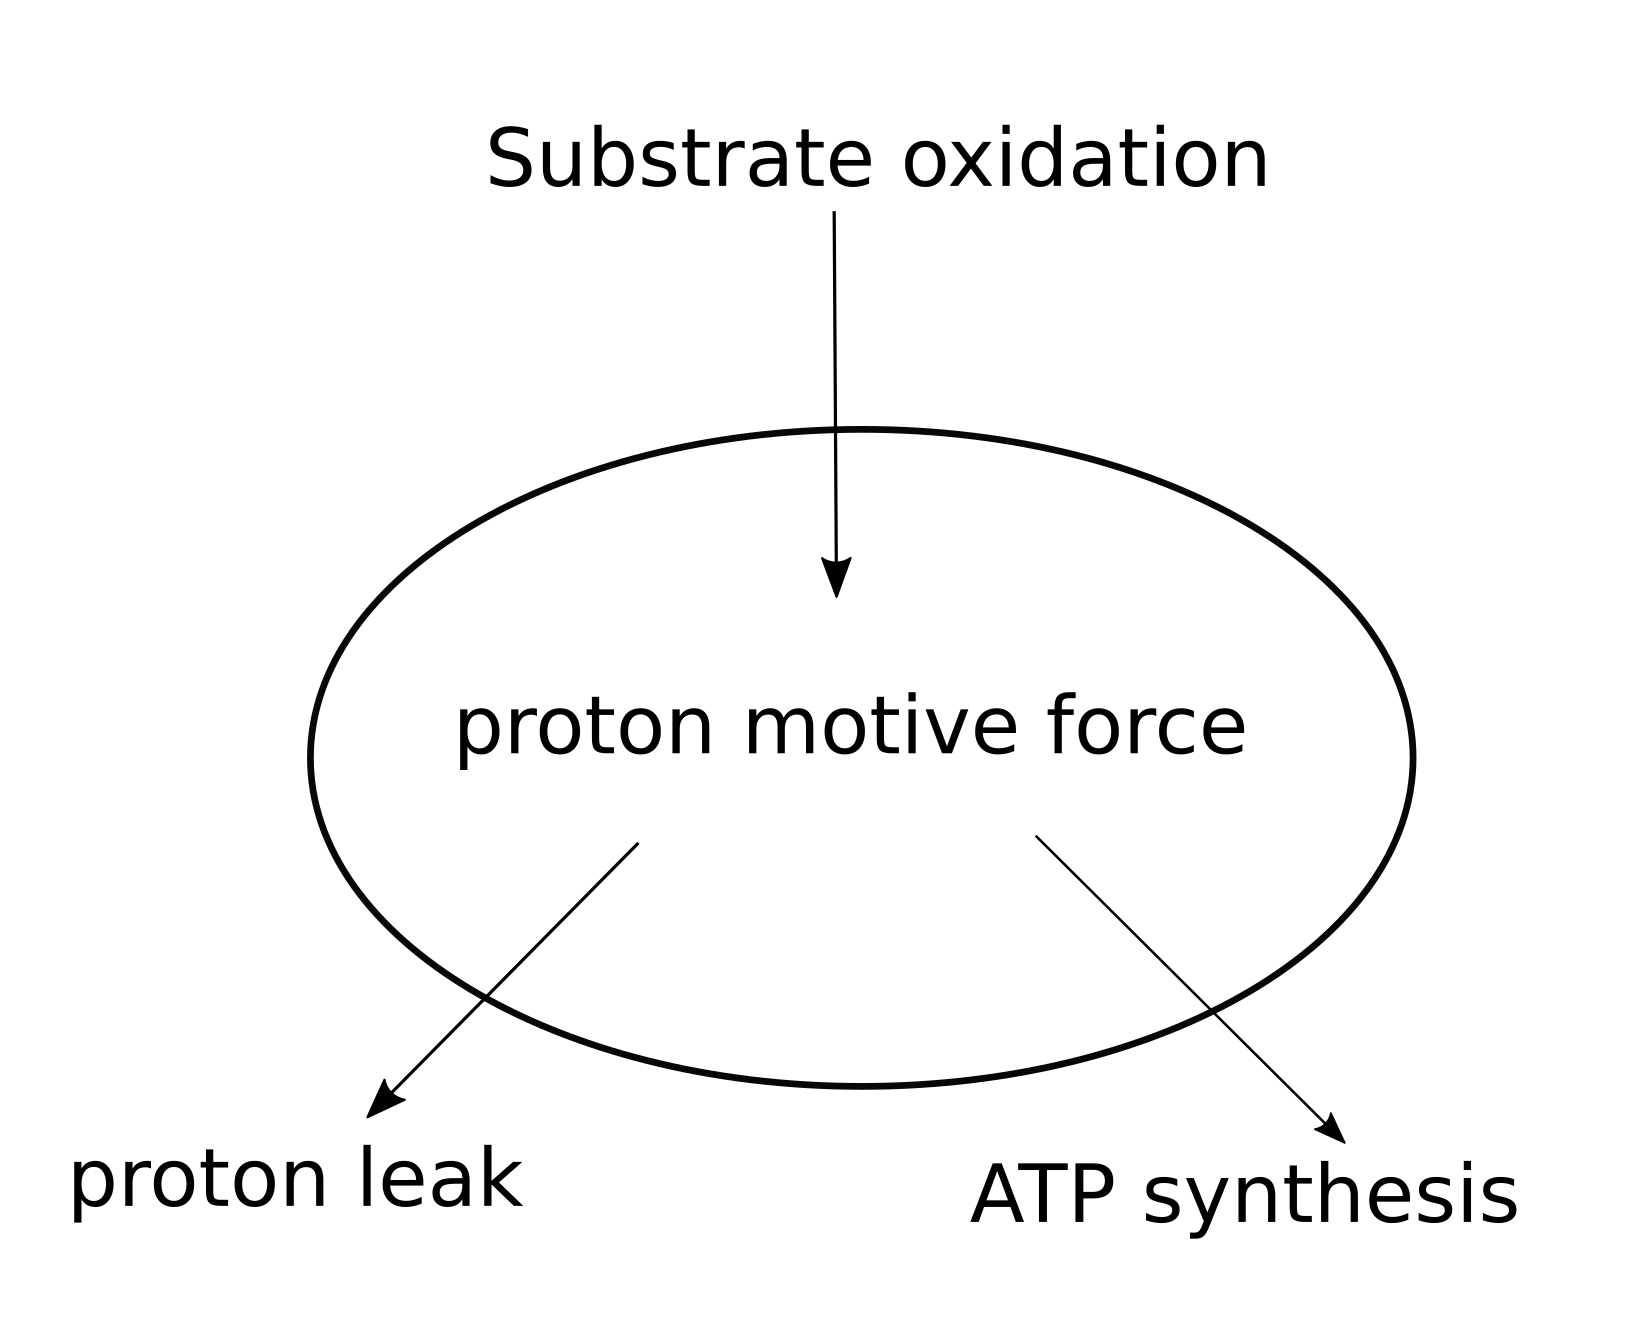
\includegraphics[width=.5\textwidth]{device}
    \caption[Components of OXPHOS respiration]{Substrate oxidation driven respiration generates proton motive force which is consumed by ATP synthesis and proton leak.\\Substrate oxidation consists of all reactions upstream of the ATP synthase, such as reactions in the ETC and those involved in substrate uptake mechanisms. ATP synthesis occurs via OXPHOS at the ATP synthase complex while proton leak consist of all reaction that consume PMF and do not generate ATP.}\label{fig:device}
\end{figure}
%

The respiratory chain of the mitochondria consists of the electron transport chain (ETC) and OXPHOS protein complexes. If we consider the ETC/OXPHOS component of the mitochondria as the 'device' (\Fref{fig:device}), we can think of the input into the device as the rate of metabolic substrate oxidation which generates the PMF. The device than uses PMF to generate ATP via phosphorylation of ADP. There are losses and shunts in the system due to proton leak, which consumes PMF but does not result in ATP synthesis. The current into this device is measured via the respiration rate. Mitochondrial respiration rate is directly related to the amount of oxygen been reduced to water at Complex IV, the terminal end of the ETC cascade. Because of the tight coupling \cite{hafner_effect_1991} between electrons entering the ETC cascade and protons pumping out of the matrix, oxygen consumption measures the proton current flowing in the ETC cascade. Proton motive force (PMF), which is composed mainly of ΔΨ \eqref{eq:pmf} is a measure of the electrochemical gradient available to drive ATP synthesis and is analogous to the voltage level of a device. Together these two assays (O$_2$ consumption and measurement of PMF/ΔΨ levels) are able to give a quantitative assessment of mitochondrial functional state \cite{brand_assessing_2011}.
%
\begin{equation}\label{eq:pmf}
\text{PMF}=\mupDelta\mupPsi-61.5\text{ΔpH}
\end{equation}

\Fref{fig:pmfo2} gives an excellent summary of how the input, output and losses/shunts of the ETC/OXPHOS machinery are related to the current-voltage characteristics of the system. As we move toward the left along the red curve (increasing substrate oxidation rate, state 4 to state 3), respiration rate rises steeply as PMF is consumed. At this maximal respiration rate (state 3, ADP present with substrate), the response of ATP synthesis to PMF is shown in the blue curve. The respiration rate is progressively inhibited via a substrate enzyme inhibitor (malonate). This blue curve shows that the amount of PMF generated is a linear function of the amount of respiration. The 'proton leak' (green curve) is similarly derived by progressively inhibiting substrate oxidation at state 4 (no ADP). PMF gradually falls as proton leak driven respiration goes to zero. This also brings up an important point of proton leak respiration: even when there is no ATP synthesis activity, endogenous substrate driven respiration still occurs to generates a PMF that is then consumed by the proton leak shunt. In other words the mitochondrial machinery keeps the respiration machinery primed with PMF to respond to a change in ATP demand. The relative proportion of respiration been consumed by ATP synthesis and proton leak as a function of respiration levels and substrate oxidation rate is shown in \Fref{fig:respratios}.

\Fref{fig:pmfo2} and \Fref{fig:respratios} show that OXPHOS is a complex process that is affected by many factors. There are therefore many ways to measure the state of OXPHOS driven respiration. The next two sections will focus on two parameters that are used to measure OXPHOS respiration in this project.

\begin{figure}[htp]
	\centering
    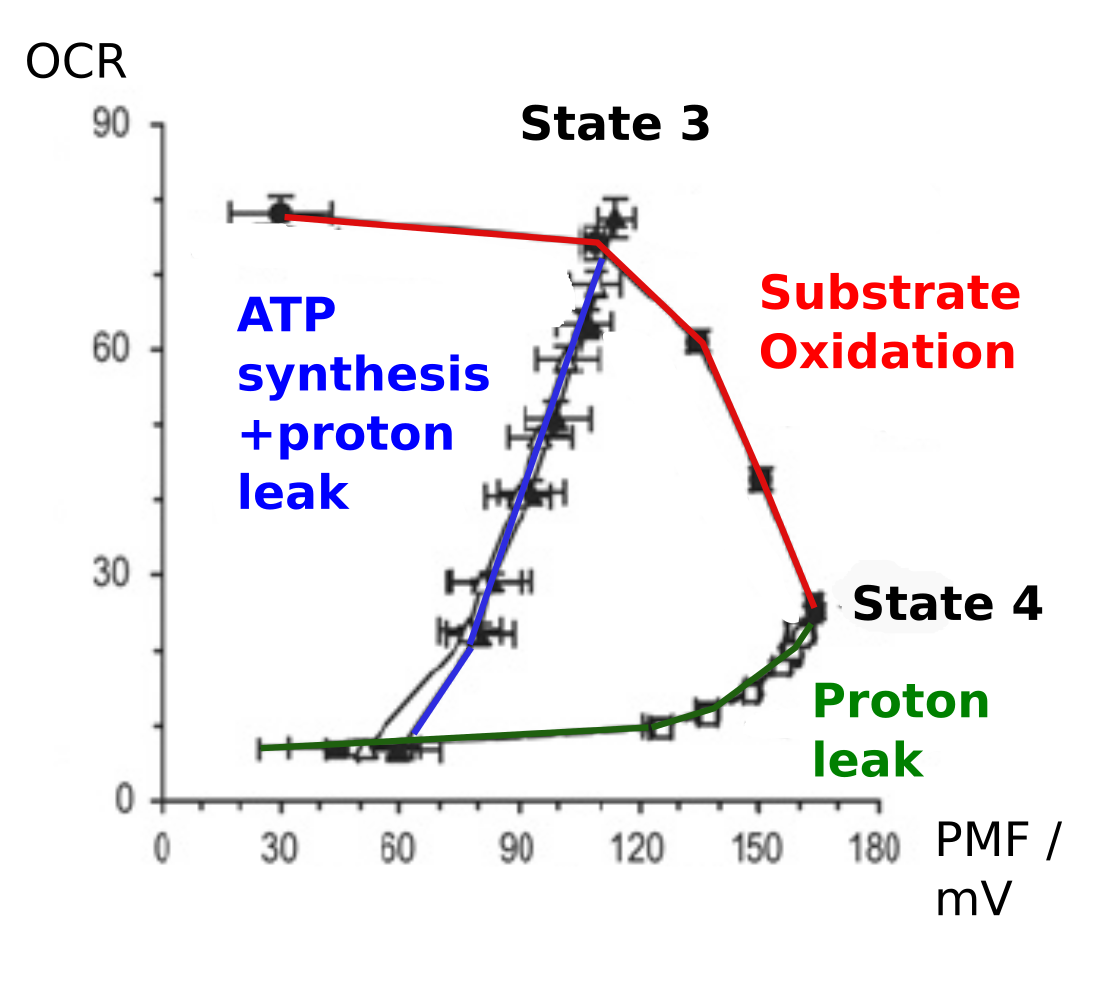
\includegraphics[width=.7\textwidth]{pmfo2}
    \caption[Respiration – PMF relationship of mitochondria]{Respiration – PMF relationship of mitochondria isolated from human lung carcinoma cells.\\Shown is response curve of substrate oxidation, proton leak respiration and ATP synthesis to PMF. The substrate given was succinate. Respiration levels were modulated via titration of FCCP for the substrate oxidation curve and malonate titration for the ATP synthesis and proton leak curves. State 3 (maximal respiration, ADP present) and State 4 (minimal respiration, no ADP) are indicated in the substrate oxidation curve. Note the linear relationship between respiration rate and PMF consumed during ATP synthesis (blue line).\\\emph{Adapted from Figure 2B of Brand et al., "Assessing mitochondrial dysfunction in cells", Biochem J 2011, used under CC BY-NC 2.5}}\label{fig:pmfo2}
\end{figure}
%
\begin{figure}[htp]
	\centering
    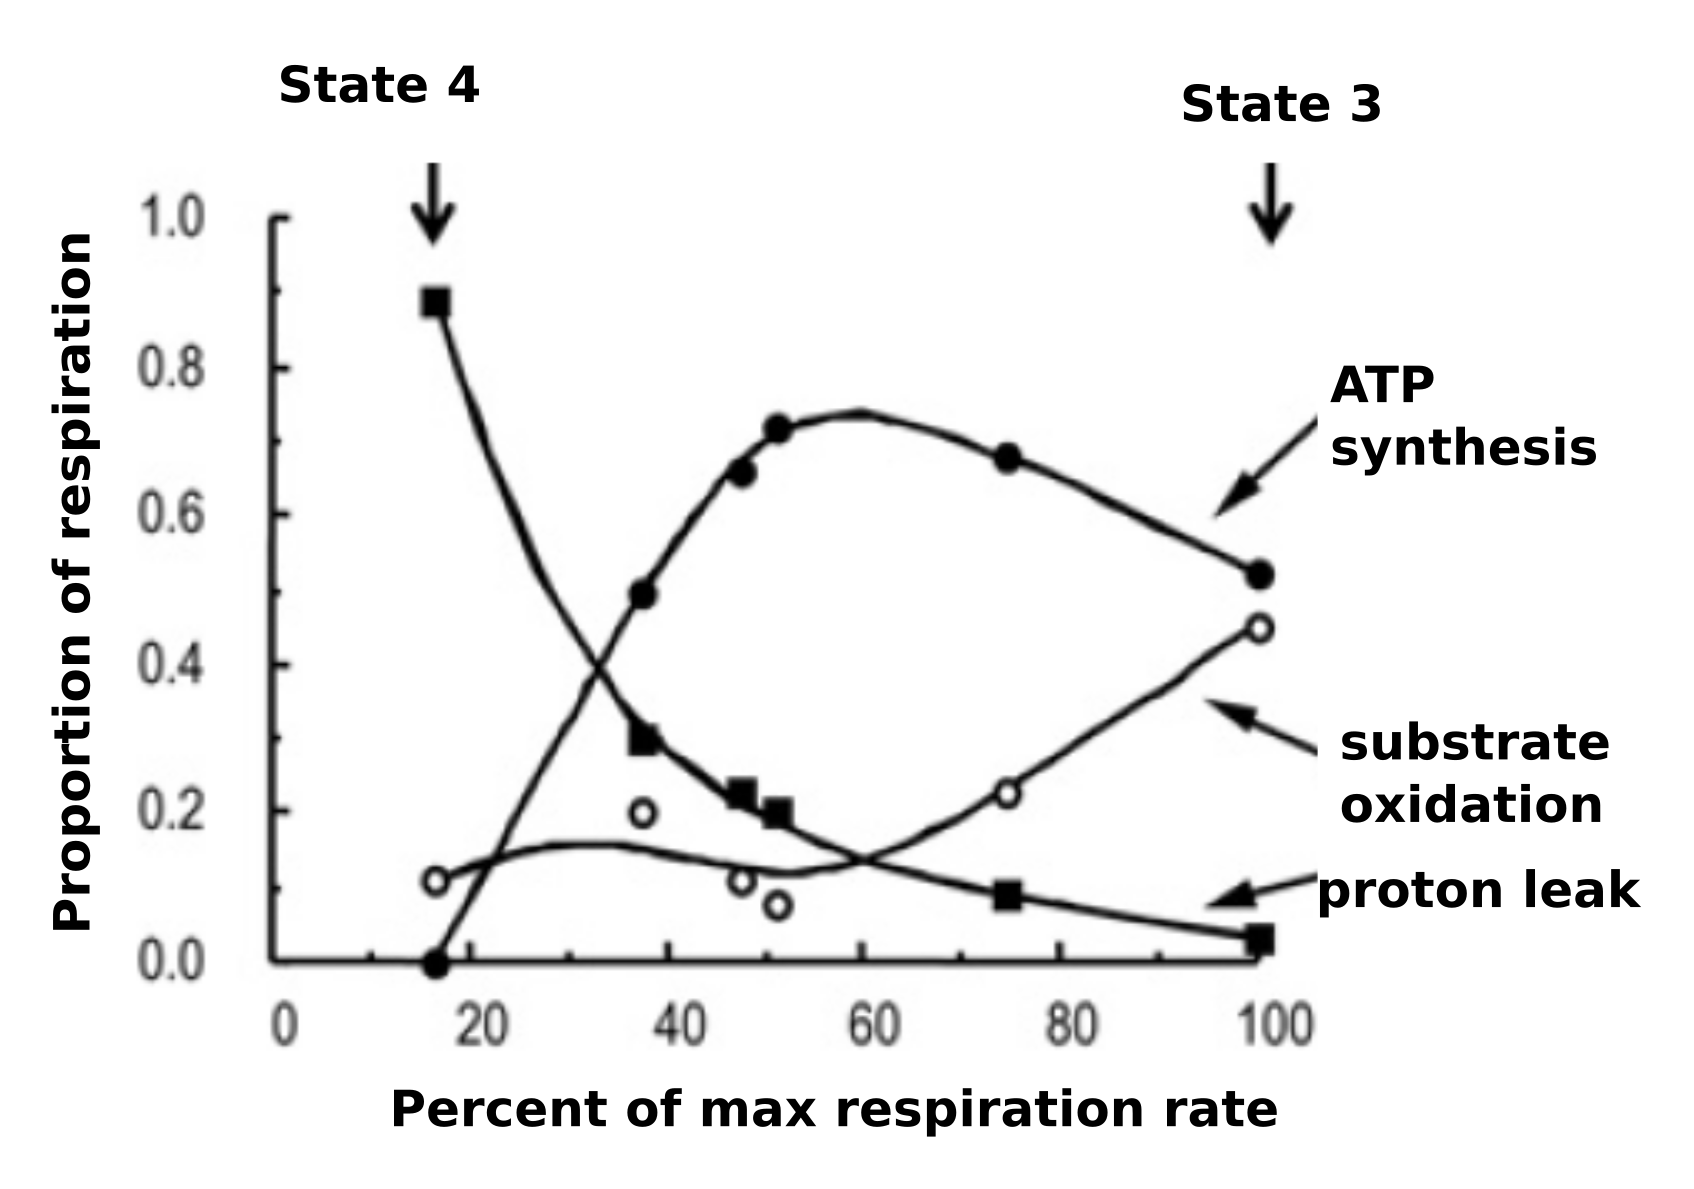
\includegraphics[width=.7\textwidth]{respratios}
    \caption[Proportion of respiration from the input and outputs of ETC/OXPHOS]{Proportion of respiration from the input and outputs of ETC/OXPHOS.\\At different respiration levels, the amount of proton leak varies depending on the level of ATP synthesis. Proton leak is maximal when ATP synthesis is zero, to maintain PMF equilibrium generated by substrate oxidation.\\\emph{Adapted from Figure 2C of Brand et al., "Assessing mitochondrial dysfunction in cells", Biochem J 2011, used under CC BY-NC 2.5}}\label{fig:respratios}
\end{figure}
%
\subsection{Mitochondrial membrane potential (ΔΨ) as a bioenergetic indicator}
Mitochondrial membrane potential (ΔΨ) is an indicator of the electrochemical gradient that is available to drive protons from the intermembrane space (IMS) into ATP synthase to phosphorylate ADP to ATP. Although respiration levels have a large gradient in relation to PMF (a large change in respiration levels results in a small PMF/ΔΨ change (\Fref{fig:pmfo2}, red curve); the use of ΔΨ as a bioenergetic indicator is still relevant. Whereas respiration measurements can only be done at a bulk level, ΔΨ measurements using fluorescent lipophilic dyes that accumulate in a Nernstian manner enable direct visualization of ΔΨ at the level of individual mitochondria \cite{twig_tagging_2006,wikstrom_-cell_2007}. In addition, mitochondrial dynamics, in particular selective fusion of mitochondrial fragments are believed to be dependent on ΔΨ \cite{twig_fission_2008}. Since fusion is believed to be affected by ΔΨ levels, one can use ΔΨ as a biomarker for function and correlate it with changes to the structure of the mitochondrial network. 
\subsection{Oxygen consumption measurement of cellular respiration}
The classic assay for cell respiration was developed by Chance and Williams \cite{chance_respiratory_1955}, using a Clark electrode to measure oxygen consumption rate (OCR) in isolated mitochondria. In this assay, isolated mitochondria are incubated with a substrate and ADP (state 3). As respiration increases the dissolved oxygen concentration decreases. The reduction of oxygen to water by the flow of electrons from the ETC generates the necessary PMF for ATP synthesis. Once ATP/ADP levels reach an equilibrium, ATP synthesis and respiration rates slow down (state 4).
%
\begin{figure}[htp]
	\centering
    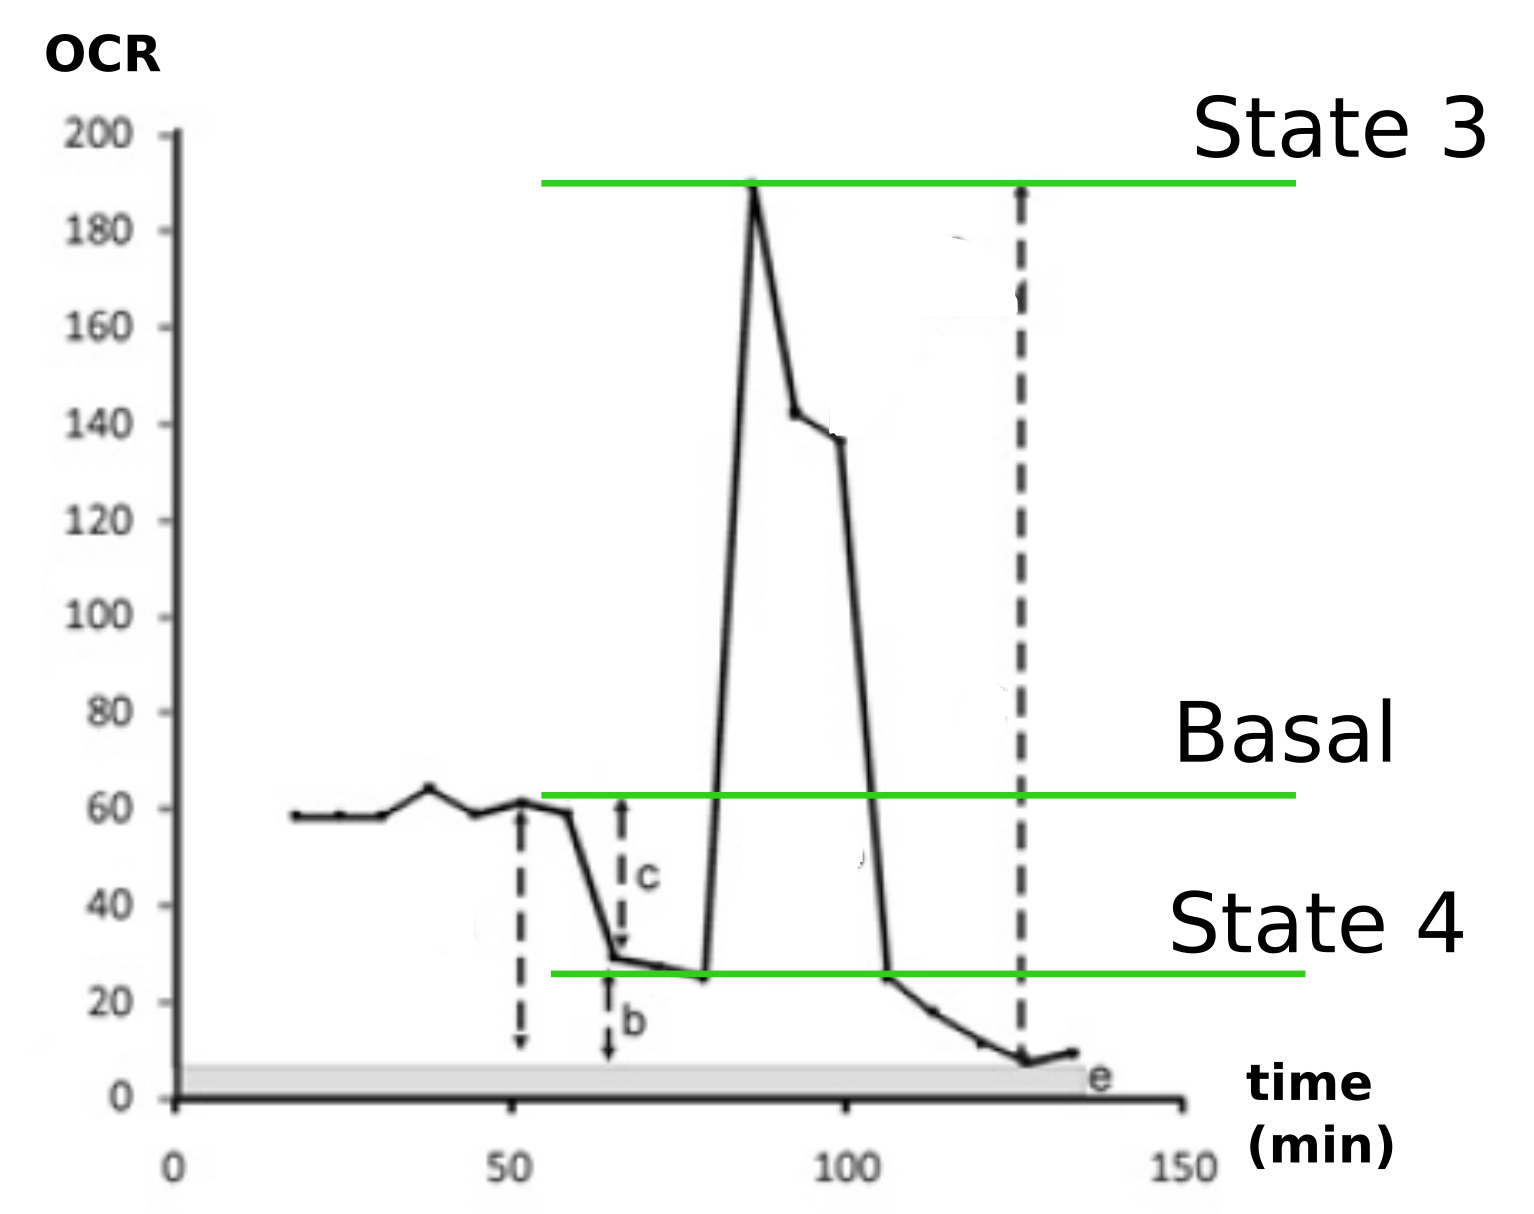
\includegraphics[width=.65\textwidth]{basal}
    \caption[Definition of State 3, basal and State 4 respiration levels]{State 3, basal and State 4 respiration levels in rat cortical neuron cells.\\State 4 is reached by addition of oligomycin from basal respiration levels. State 3 is reached by addition of a protonophore, FCCP from State 4. Respiratory control ratio is the ratio of state 3 to state 4 respiration level, spare respiratory capacity is State 3 minus basal level respiration.\\\emph{Adapted from Figure 3A of Brand et al., "Assessing mitochondrial dysfunction in cells", Biochem J 2011, used under CC BY-NC 2.5}}\label{fig:basal}
\end{figure}
%

In intact cells, state 3 can be approximated by the addition of a protonophore such as FCCP, to allow uncoupled (not tied to OXPHOS) maximal respiration (\Fref{fig:basal}). State 4 can be approximated by the addition of oligomycin to inhibit the ETC cascade. Any respiration detected in state 4 is due to 'leak' respiration (respiration due to protons reentering directly into the matrix). We used the Clark electrode method to measure basal respiration in this study. In intact cells, basal respiration corresponds to a state intermediate between State 3 (unlimited substrate and ADP, maximum respiration) and State 4 (unlimited substrate, no ATP synthesis, minimal respiration).
\subsection{Variation of carbon source substrates and their expected bioenergetic measurements}\label{sec:carbon}
In the context of this project, we wanted to study the change of structure and function in the mitochondrial network in one metabolic state (fermentation) compared to another (respiration). Therefore we grew yeast cells in different carbon sources to obtain:
\begin{enumerate}[label=\emph{\alph*}), leftmargin=*, itemindent=0pc]
\item glucose repressing conditions (2\% glucose)
\item fermentable, non repressing conditions (2\% raffinose)
\item Non-fermentable carbon substrates (2\% lactate and 2\% glycerol + 2\% ethanol). The use of two different non-fermentable carbon substrates was due to the fact that glycerol enters the glycolytic pathway, and though it is usually considered a non-fermentable substrate we decided to include lactate which completely bypasses the glycolytic pathway. 
\end{enumerate}
Based on the above review and our understanding of how each of the different carbon sources are metabolized, we expected cells grown in glucose to have the lowest OCR and ΔΨ due to the glucose repression effect. The non-fermentable carbon substrates (lactate and glycerol+ethanol) were expected to have the highest OCR and ΔΨ due to the cells having to undergo aerobic respiration. Raffinose was expected to have intermediate levels of OCR and ΔΨ as it is able to undergo simultaneous fermentation and respiration.
\section{Materials and Methods}
\subsection{\texorpdfstring{O\textsubscript{2}}{O2} consumption rate measurement using a Clark electrode}
The Clark type electrode measures oxygen on a catalytic platinum surface \cite{li_measurement_2012}. The system consists of a platinum cathode and silver anode, bridged by a potassium chloride electrolyte (\Fref{fig:clark}). An oxygen permeable membrane separates the electrode from a sealed chamber containing the liquid sample to be measured. The platinum cathode is reduced by oxygen diffusing through the membrane. The current is proportional to the oxygen concentration in the solution. At the silver anode, the circuit is completed by the precipitation of silver chloride from the ions at the anode. An analog to digital converter unit records the current that represents the oxygen concentration in the sample.
%
\begin{figure}[htp]
	\centering
    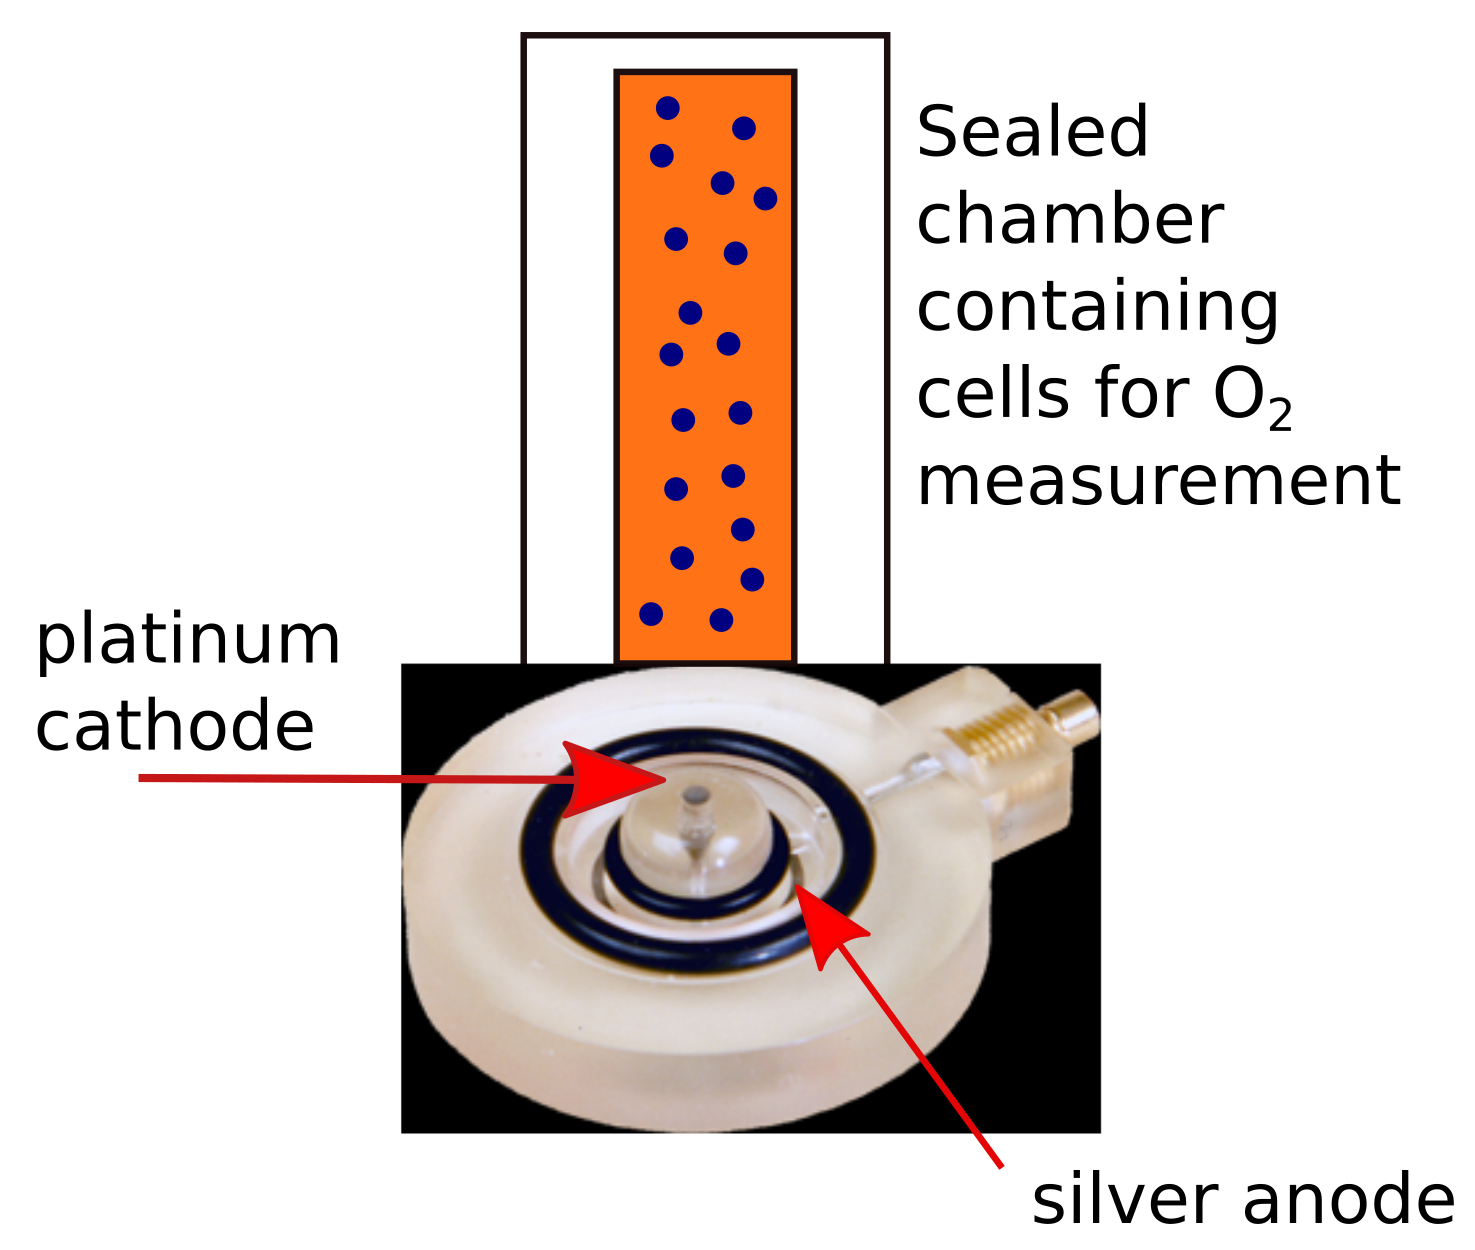
\includegraphics[width=.7\textwidth]{clark}
    \caption[Diagram of a Clark electrode used for oxygen consumption rate (OCR) measurement]{Diagram of a Clark electrode used for oxygen consumption rate (OCR) measurement.\\
A PTFE oxgyen permeable membrane covers the platinum cathode and separates the cathode from the sample. An electrolyte soaked wicking paper, which lies underneath the membrane serves as an electrolytic bridge from the cathode to the anode. The current generated at the cathode is directly proportional to the oxygen concentration in the sample (cells shown as blue dots), which is enclosed by a sealed chamber (orange and white rectangle).}\label{fig:clark}
\end{figure}
%

Oxygen consumption of yeast cells grown in the following media were measured in a Clark oxygen electrode chamber (Oxytherm, Hansatech Instruments): Yeast extract + peptone (YP) + glucose 2\% (YPD), YP + 2\% glycerol + 2\% ethanol (YPE), YP + 2\% lactate (YPL), YP + 2\% raffinose. Measurements of each condition consisted of 6--10 runs over 2 days (total N=14--20). Oxygen consumption rate (OCR) was reported as \si{\OCR}. We normalized OCR by dry weight of cell as well as by cell number and mitochondrial volume.
\subsection{OCR measurement protocols}
\begin{enumerate}[label=\arabic*), leftmargin=*, itemindent=0pc]
\item Cells were grown in suspension to log phase (details in \fref{sec:loaddye})
\item Setup and calibration of the electrode was performed on the day of the experiment using the instructions from the manufacturer. A 50\% potassium chloride solution was pipetted onto the platinum cathode and then covered with a PTFE membrane. The electrode chamber was filled with aerated water and flushed with nitrogen gas to establish a zero baseline measurement. Calibration was done at room temperature (22°C).
\item\label{itm:3} Starting from the lowest optical density (OD$_{600}$) reading (typically \textasciitilde0.25), a 1 ml cell suspension was pipetted into the electrode chamber. The reading was then taken for between 2--5 minutes. The OCR at that particular OD$_{600}$ was measured as the slope of the linear part of the curve (between the red lines in \Fref{fig:linear}) and expressed as \si{\OCR}. After every measurement the cells were aspirated and the chamber flushed with clean water.
Step \ref{itm:3} was repeated for increasing OD$_{600}$ readings up to about OD$_{600}$ of about 0.5.  The maximum OD$_{600}$ was limited by the fact that as the cell density increased in the chamber, the length of time for which a linear part of the curve can be obtained was decreased. The maximum OD$_{600}$ for each condition was around 0.5--0.6. A curve for OCR as a function of cell optical density OD$_{600}$ was then fitted (\Fref{fig:OCRraw}). The shaded bands represent the bootstrapped 95\% confidence intervals of the fitted OCR values.
\item OCR normalized to unit mass of cells was obtained by measuring the dry mass of cells at an OD$_{600}$ of approximately 0.5 for each of the experimental growth conditions. Cell mass was obtained by growing \textasciitilde{8 ml} of yeast cell culture in a weighted conical glass tubes (Corning 99502-15), to an OD$_{600}$ of approximately 0.5. The glass tube was then centrifuged for 15 minutes at 3000g to pellet the cells and the supernatant discarded. The glass tube was then oven dried at 70°C for two to three days. The glass tube was weighed again and the dry mass of cell obtained by taking the difference of the two weights, expressed as \si{\mg\per\ml} normalized to OD$_{600}$=0.5.  All dry weight measurements were repeated at least 5 times.
\item OCR was also normalized to cell number per ml at OD$_{600}$=0.5. Cell number was obtained by growing yeast cells to about OD$_{600}$=0.5. A \SI{1}{\ul} sample was placed into a hematocytometer (model 3100, Hausser Scientific, PA) and a cover slip was placed over the chamber. The counting chamber consisted of a predefined volume of liquid \SI{.1}{\ul}. The central square in the hematocytometer consisted of a volume of \SI{.004}{\ul}. The square was ruled into 25 groups, so each group held a volume of \SI{.00025}{\ul}. The cells were counted using 5 of the 25 groups in the central square. The average of these five reading were then multiplied by 250,000 to obtain a cell count per ml. This number was than normalized to the OD$_{600}$ it was taken at (\textasciitilde0.5) to obtain an average number of cells per ml per unit OD$_{600}$ reading. All cell counts were repeated at least 6 times.
\item OCR was also normalized to average mitochondrial volume for a particular growth condition. The average mitochondrial volume was calculated from MitoGraph v2.0 by taking the mean total length of the mitochondrial network for that cell condition (N\textasciitilde100) and multiplying by the cross section, assuming a constant mitochondrial tubule diameter of \SI{300}{\nm}. For all three methods of normalization (OCR normalized by dry weight, cell number and mitochondrial volume), the error bars shown in (\Fref{fig:O2bars}) represent the 95\% confidence interval obtained by bootstrapping 1000 samples of the normalized OCR measurement and the height of the bars represent the median value for the normalized OCR at OD$_{600}$=0.5.
\end{enumerate}
%
\begin{figure}[htp]
	\centering
    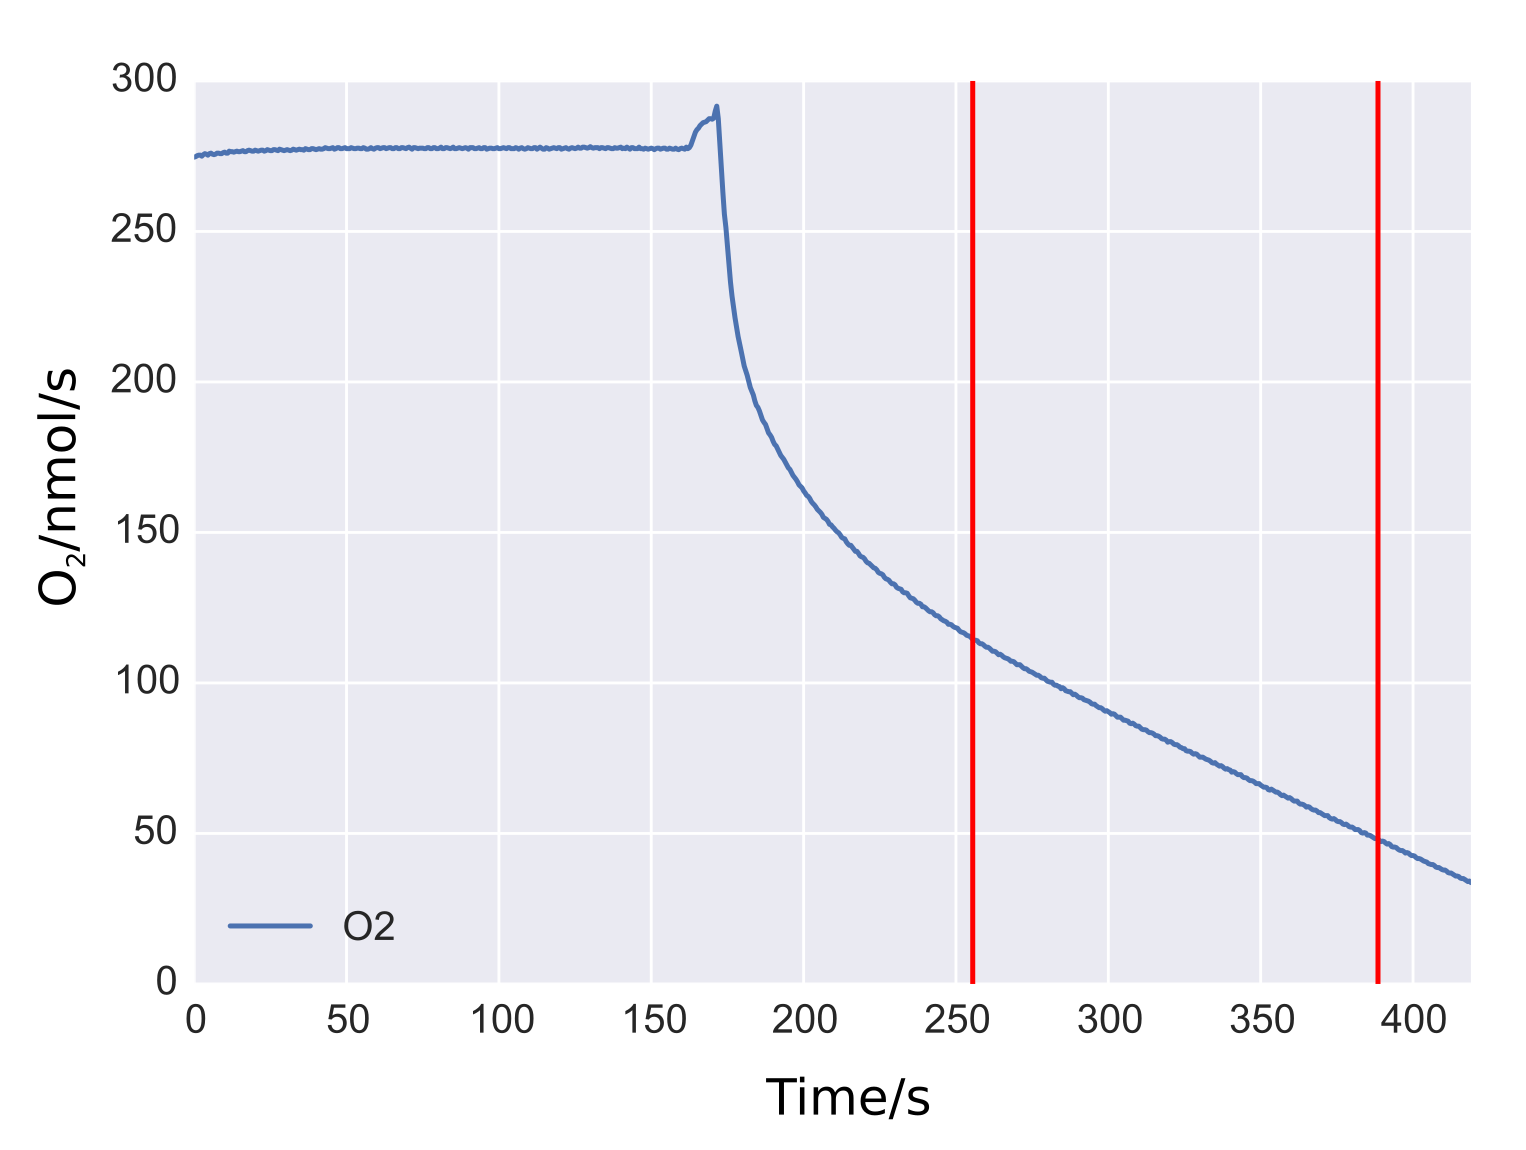
\includegraphics[width=.65\textwidth]{linear}
    \caption[Raw oxygen consumption rate (OCR) data from one sampling run at a particular carbon source and OD$_{600}$ reading.]{Raw oxygen consumption rate (OCR) data from one sampling run at a particular carbon source and OD$_{600}$ reading.\\A Clark electrode was used to measure OCR of live yeast cells grown at various concentrations (measured as optical density, OD$_{600}$). For a particular sampling run, the OCR was calculated as the slope of the linear region (between the two vertical red lines). Multiple sampling runs at different OD$_{600}$ readings are repeated to obtain the curve fit shown in \Fref{fig:OCRraw}}\label{fig:linear}
\end{figure}
%
%
\begin{figure}[htp]
	\centering
    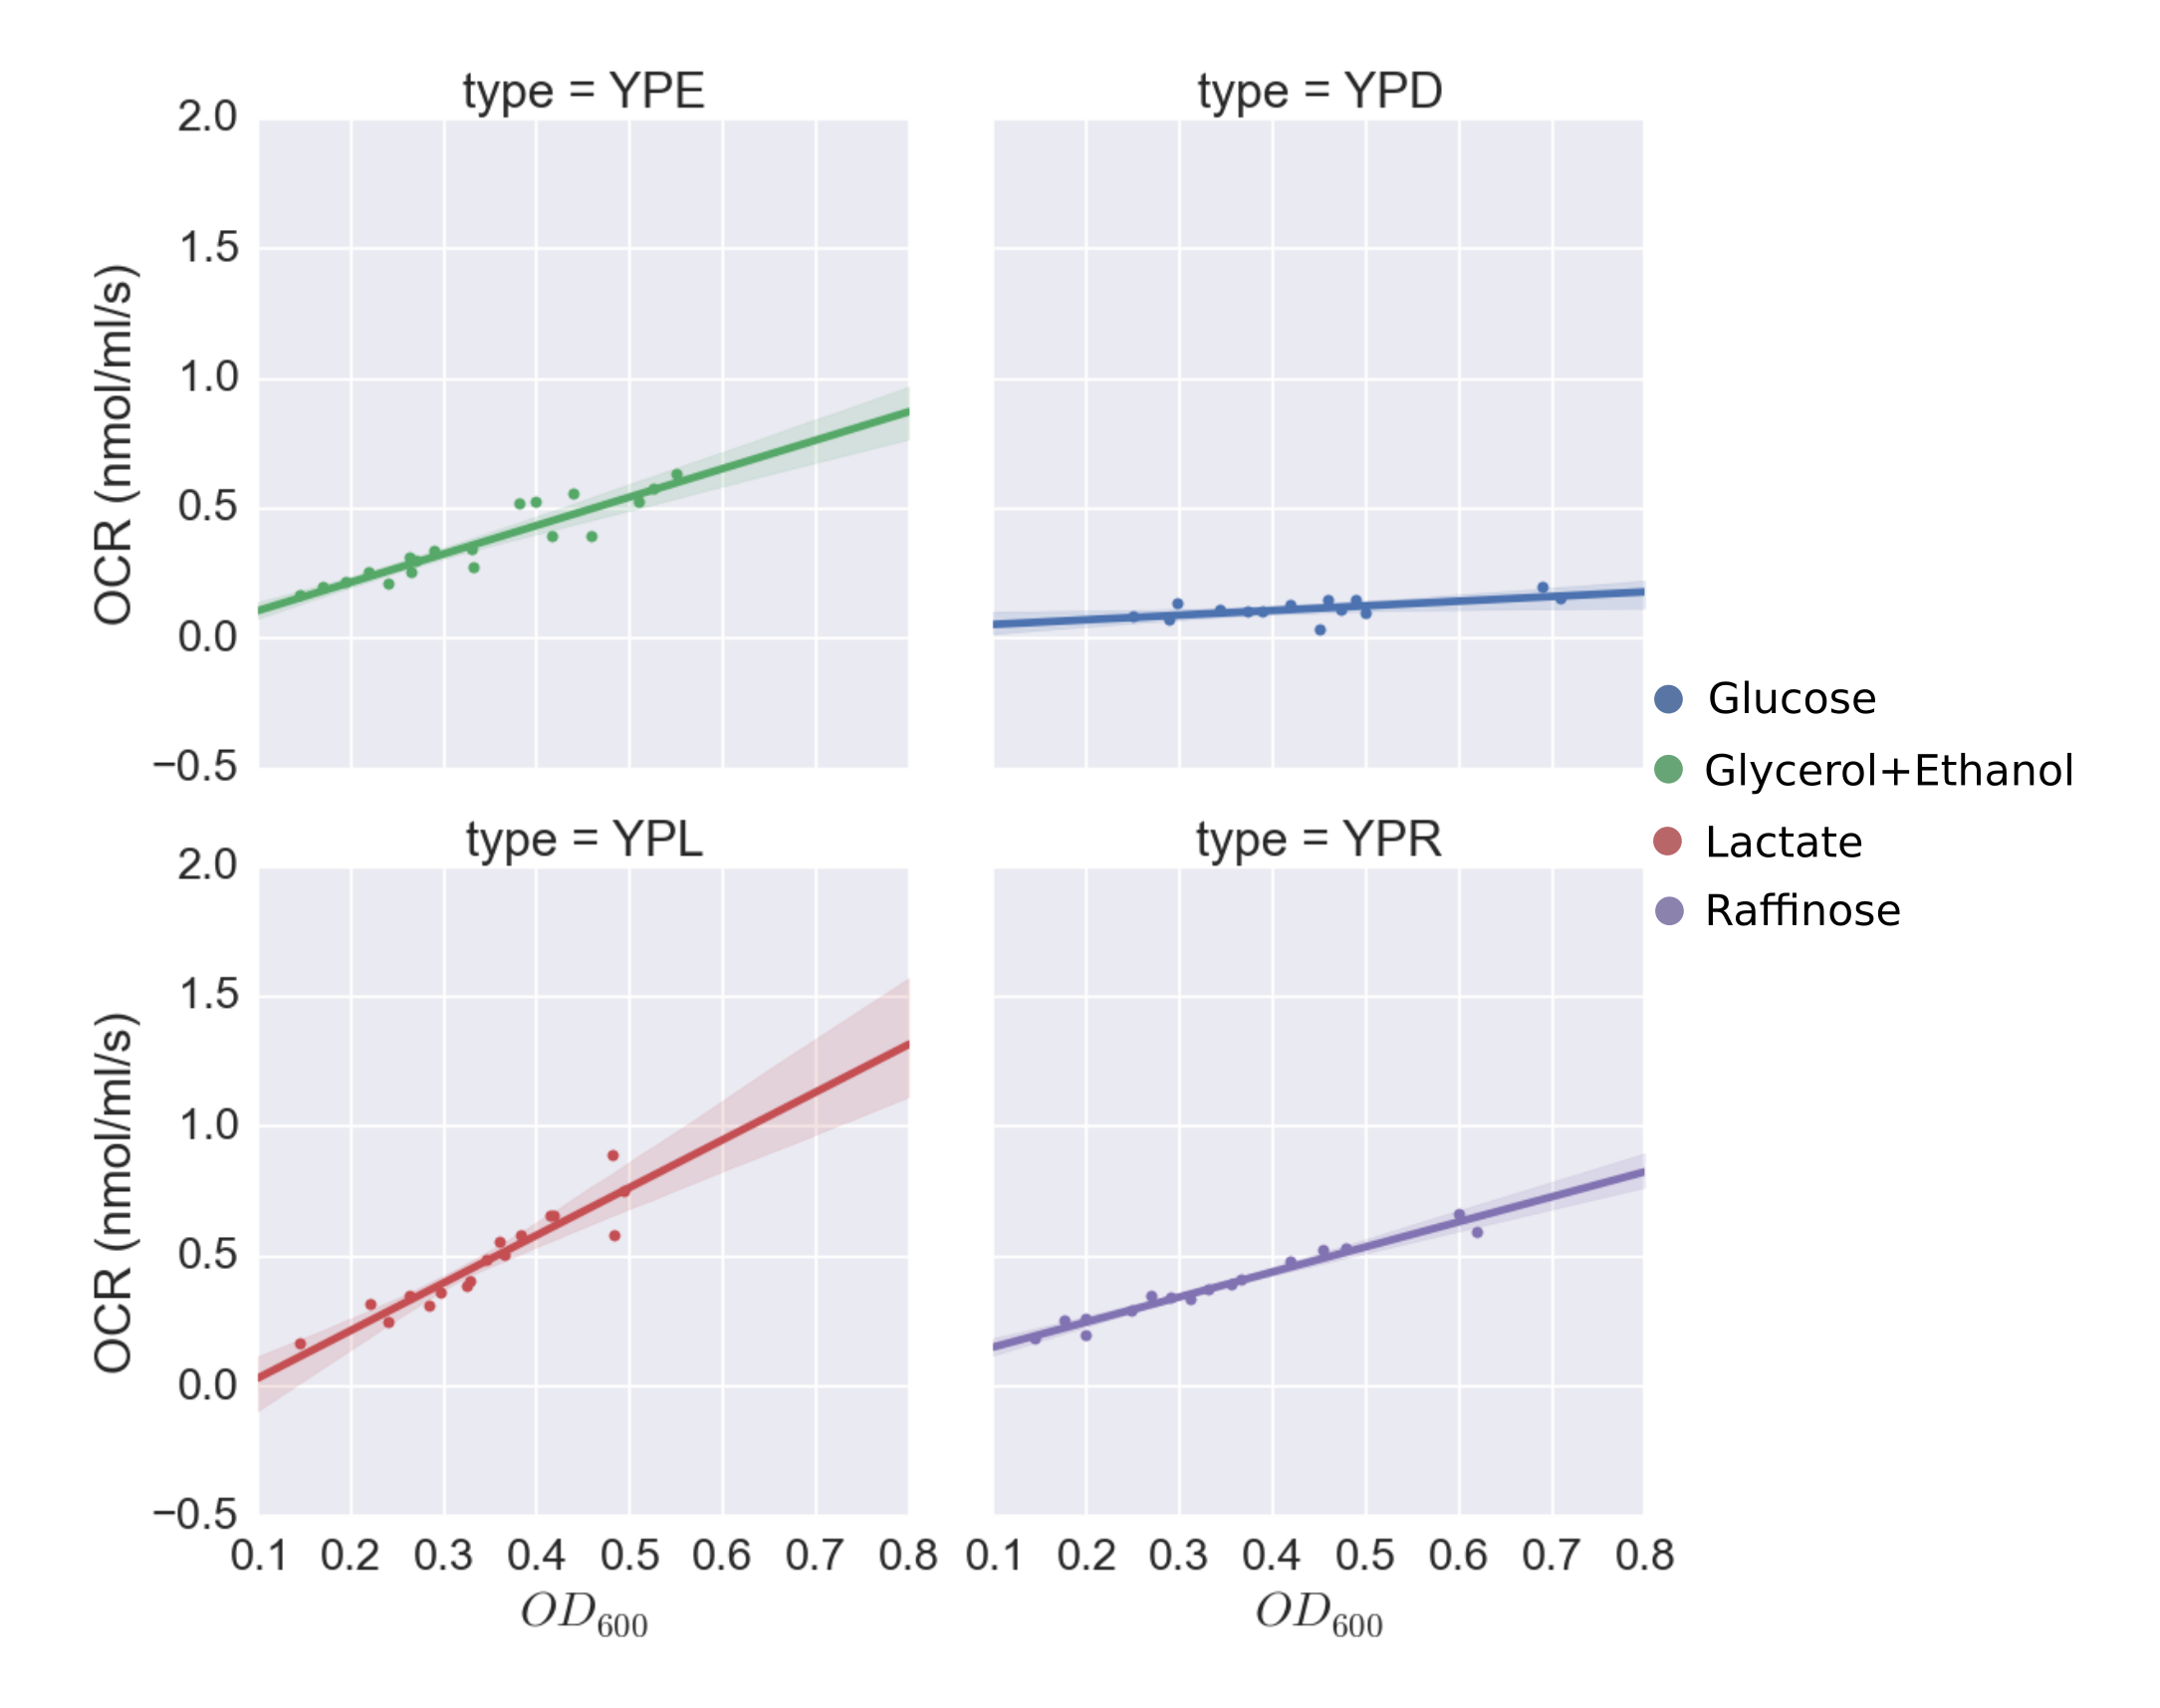
\includegraphics[width=\textwidth]{OCRraw}
    \caption[Respiration rate (OCR) as a function of optical density (OD$_{600}$).]{Respiration rate (OCR) as a function of optical density (OD$_{600}$).\\OCR readings from multiple sampling runs at different cell concentrations (OD$_{600}$) were plotted for cells grown in various carbon sources. The curve fit allows one to obtain the OCR at the OD$_{600}$=0.5 which we used as the standard OD reading to obtain normalized OCR by mass, cell number and mitochondrial volume.\\
\emph{Shaded band represent the bootstrapped 95\% confidence interval for the fitted values.}}\label{fig:OCRraw}
\end{figure}
%
%
\begin{figure}[htp]
	\centering
    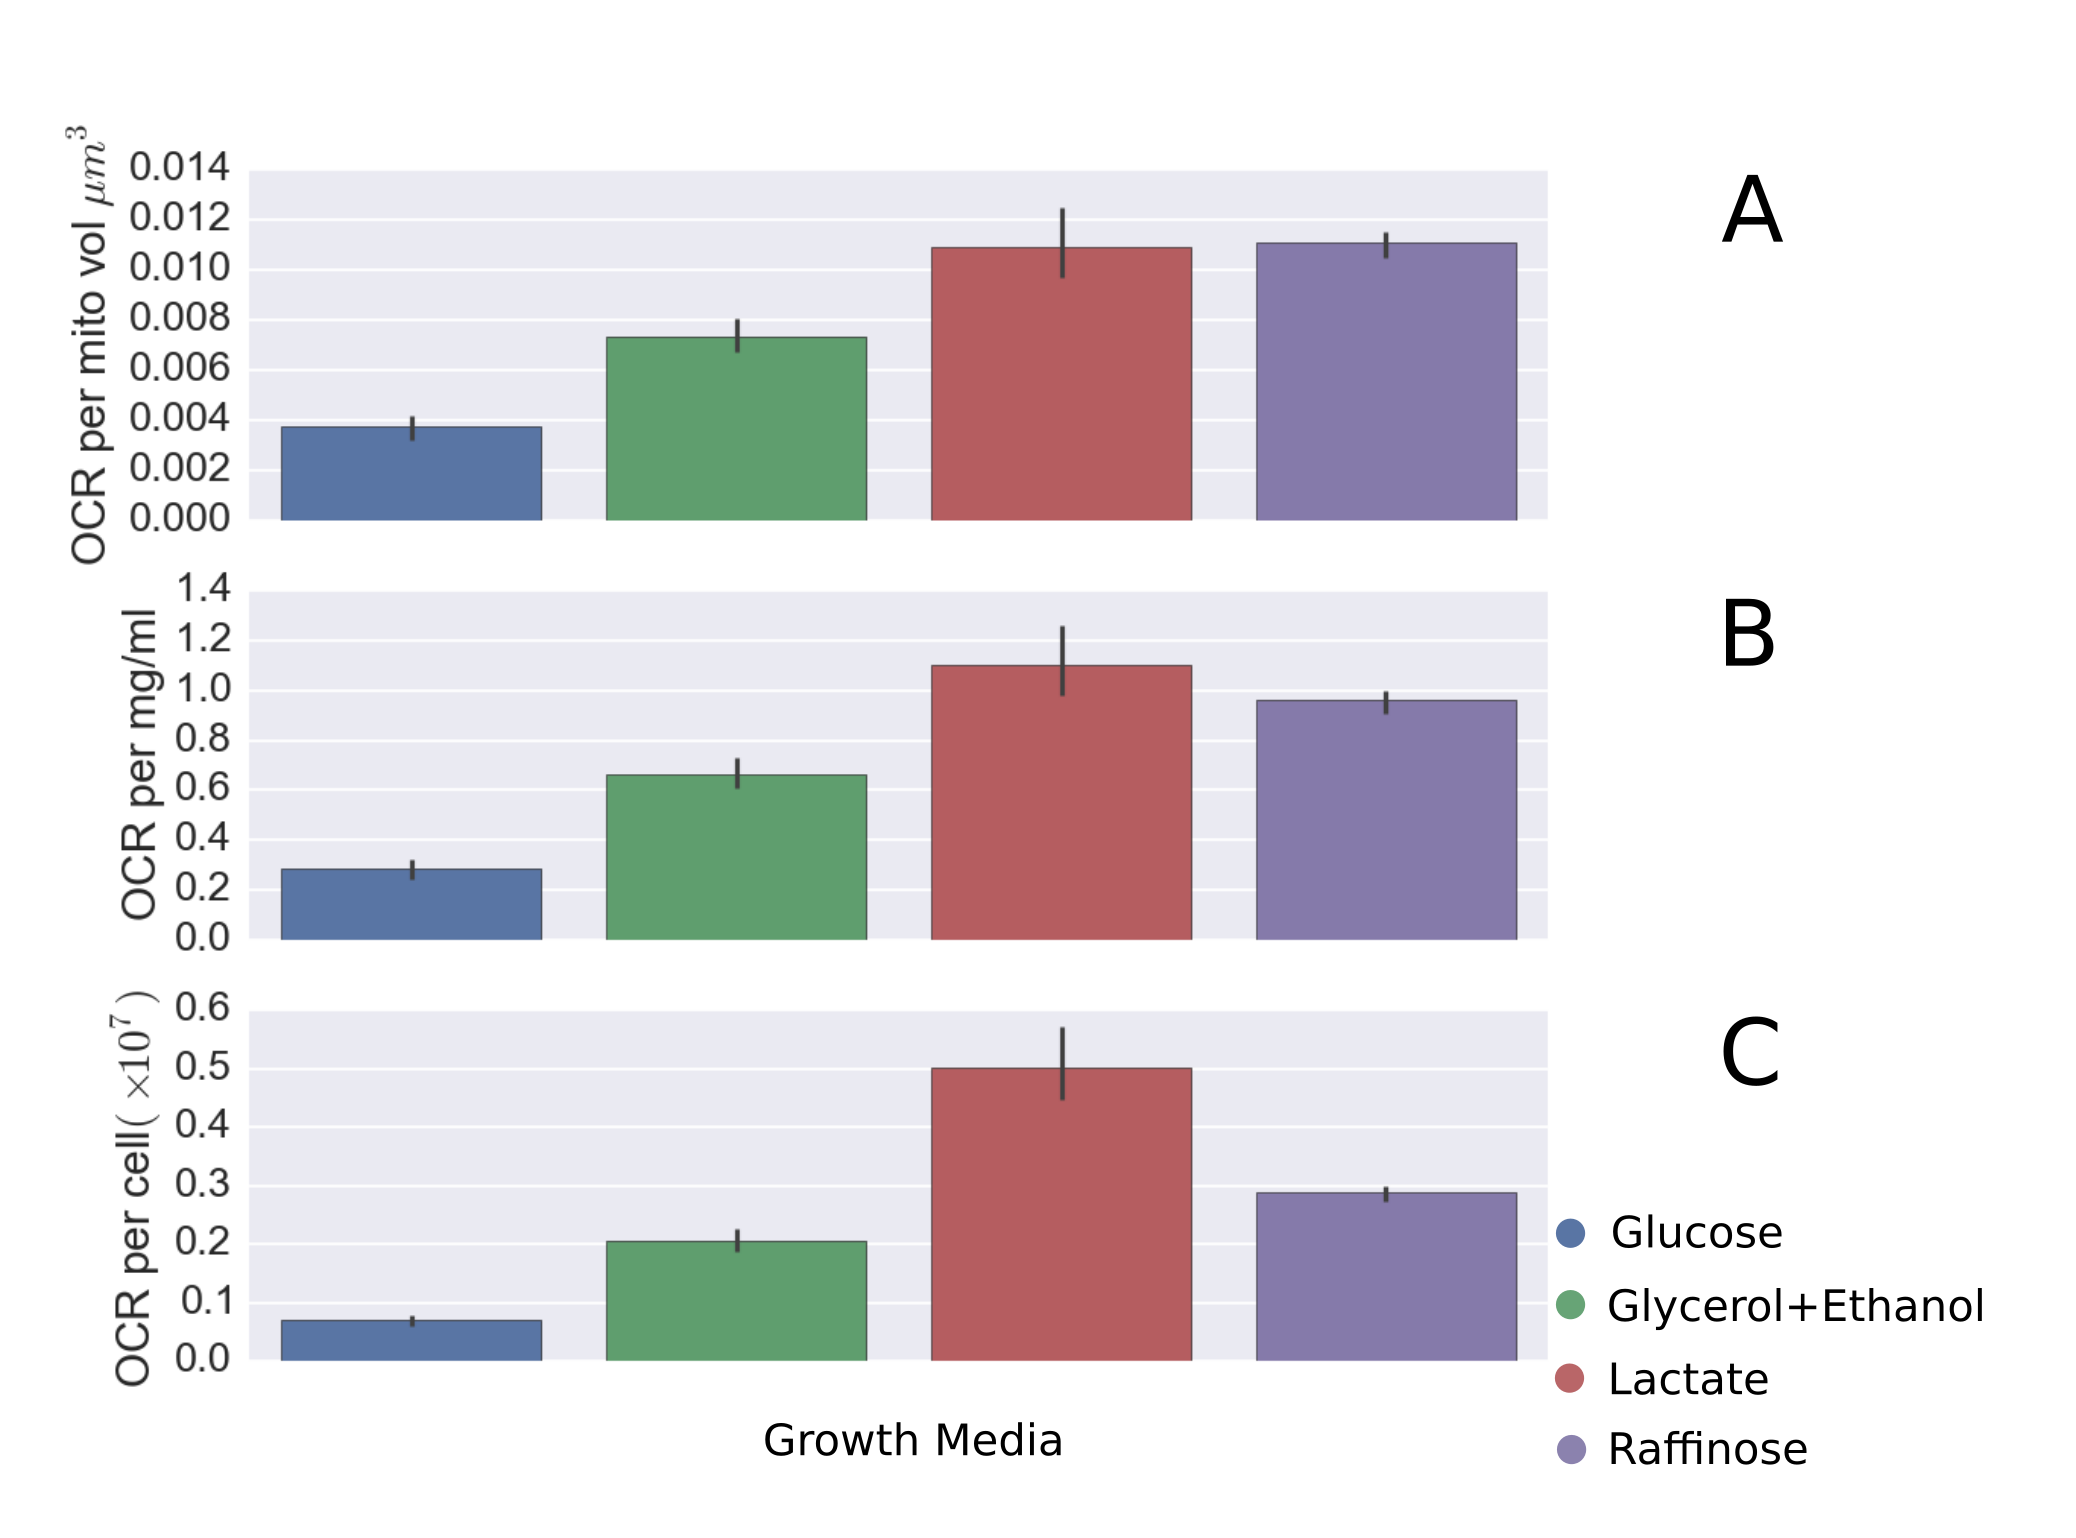
\includegraphics[width=\textwidth]{o2bars}
     \subcaptionbox{OCR normalized by mitochondrial volume\label{fig:O2barsA}}[\linewidth]{}
      \subcaptionbox{OCR normalized by dry mass\label{fig:O2barsB}}[\linewidth]{}
       \subcaptionbox{OCR normalized by number of cells\label{fig:O2barsC}}[\linewidth]{}
    \caption[Oxygen consumption rate (OCR) of yeast in different carbon sources.]{Oxygen consumption rate (OCR) of yeast in different carbon sources.\\OCR readings of yeast cells from sample volumes of 1 ml at OD$_{600}$=0.5 were normalized by mitochondrial volume (A), dry mass (B) or cell number (C). Different normalization methods result in different rankings of mitochondrial OCR in the different carbon sources. However mitochondria grown in glucose (fermentation condition) consistently showed the lowest mitochondrial OCR due to glucose repression. OCR normalized by mitochondrial volume is the most appropriate way to compare mitochondrial respiration rate as mitochondrial volume is a direct measurement of the amount of mitochondria in the sample volume. The other two methods scale not just with the amount of mitochondria in the sample volume but also cell size and numbers. OCR in glycerol+ethanol showed a two fold higher normalized OCR rate (\Fref{fig:O2barsA}) compared to glucose, while lactate and raffinose show a three fold higher normalized OCR rate compared to glucose.\\\emph{Error bars indicate the bootstrapped 95\% confidence interval of the median OCR value.}}\label{fig:O2bars}
\end{figure}
%
\section{Results}
We report OCR normalized in three different ways (\Fref{fig:O2bars}). \Fref{fig:O2barsA} shows the result of OCR in the different carbon conditions, normalized by mitochondrial volume. The other two subfigures show two standard ways OCR measurement in intact cells are usually reported in the literature, which are normalization by dry mass (\Fref{fig:O2barsB}) and cell number (\Fref{fig:O2barsC}). The OCR differences between the carbon conditions are similar regardless of the normalization methods except for the case of raffinose. In all cases glucose has the lowest OCR, lactate the highest and glycerol+ethanol intermediate between the two. Raffinose shows a respiration rate that is either similar to lactate (A and B) or lower than lactate but still higher than glycerol+ethanol. For the OCR normalized by mitochondrial volume measurements, cells grown in glycerol+ethanol showed a two fold increase in OCR levels compared to those in glucose (fermentation only conditions). Cells grown in lactate and raffinose show a three fold increase in OCR levels (lactate and raffinose had no significant difference in their OCR rate normalized to mitochondrial volume, evidenced by the error bars overlapping in \Fref{fig:O2barsA}).

We believe OCR normalized to total mitochondrial volume calculated from MitoGraph v2.0 is the most specific measure to show how mitochondrial respiration is affected by changes in growth conditions. Normalization by cell number does not account for changes in the proportion of the cell volume that is occupied by mitochondria (volume ratio) between different growth conditions. It cannot differentiate increased respiration due to there been more cells or because the cells have increased mitochondrial volume ratio. Normalizing by dry mass of cell also suffers from this problem; it cannot differentiate increased respiration due to there been more cells, and hence total mass or if specific cell mass increased due to increased mitochondrial volume ratio (or even if specific cell mass increased due to non mitochondrial content). An alternative OCR normalization method is normalizing by mitochondrial associated protein content.

The OCR levels for raffinose was surprising as we predicted it would be intermediate between the non-fermentable glycerol+ethanol and glucose substrates. Furthermore, ΔΨ levels did not correlate perfectly with OCR for the case of raffinose, glycerol+ethanol and lactate (\Fref{fig:O2dy}). Cells grown in glycerol+ethanol displayed the highest average ΔΨ level while having OCR intermediate between glucose and lactate/raffinose. These unexpected results are discussed further in the next section.
%
\begin{figure}[htp]
	\centering
    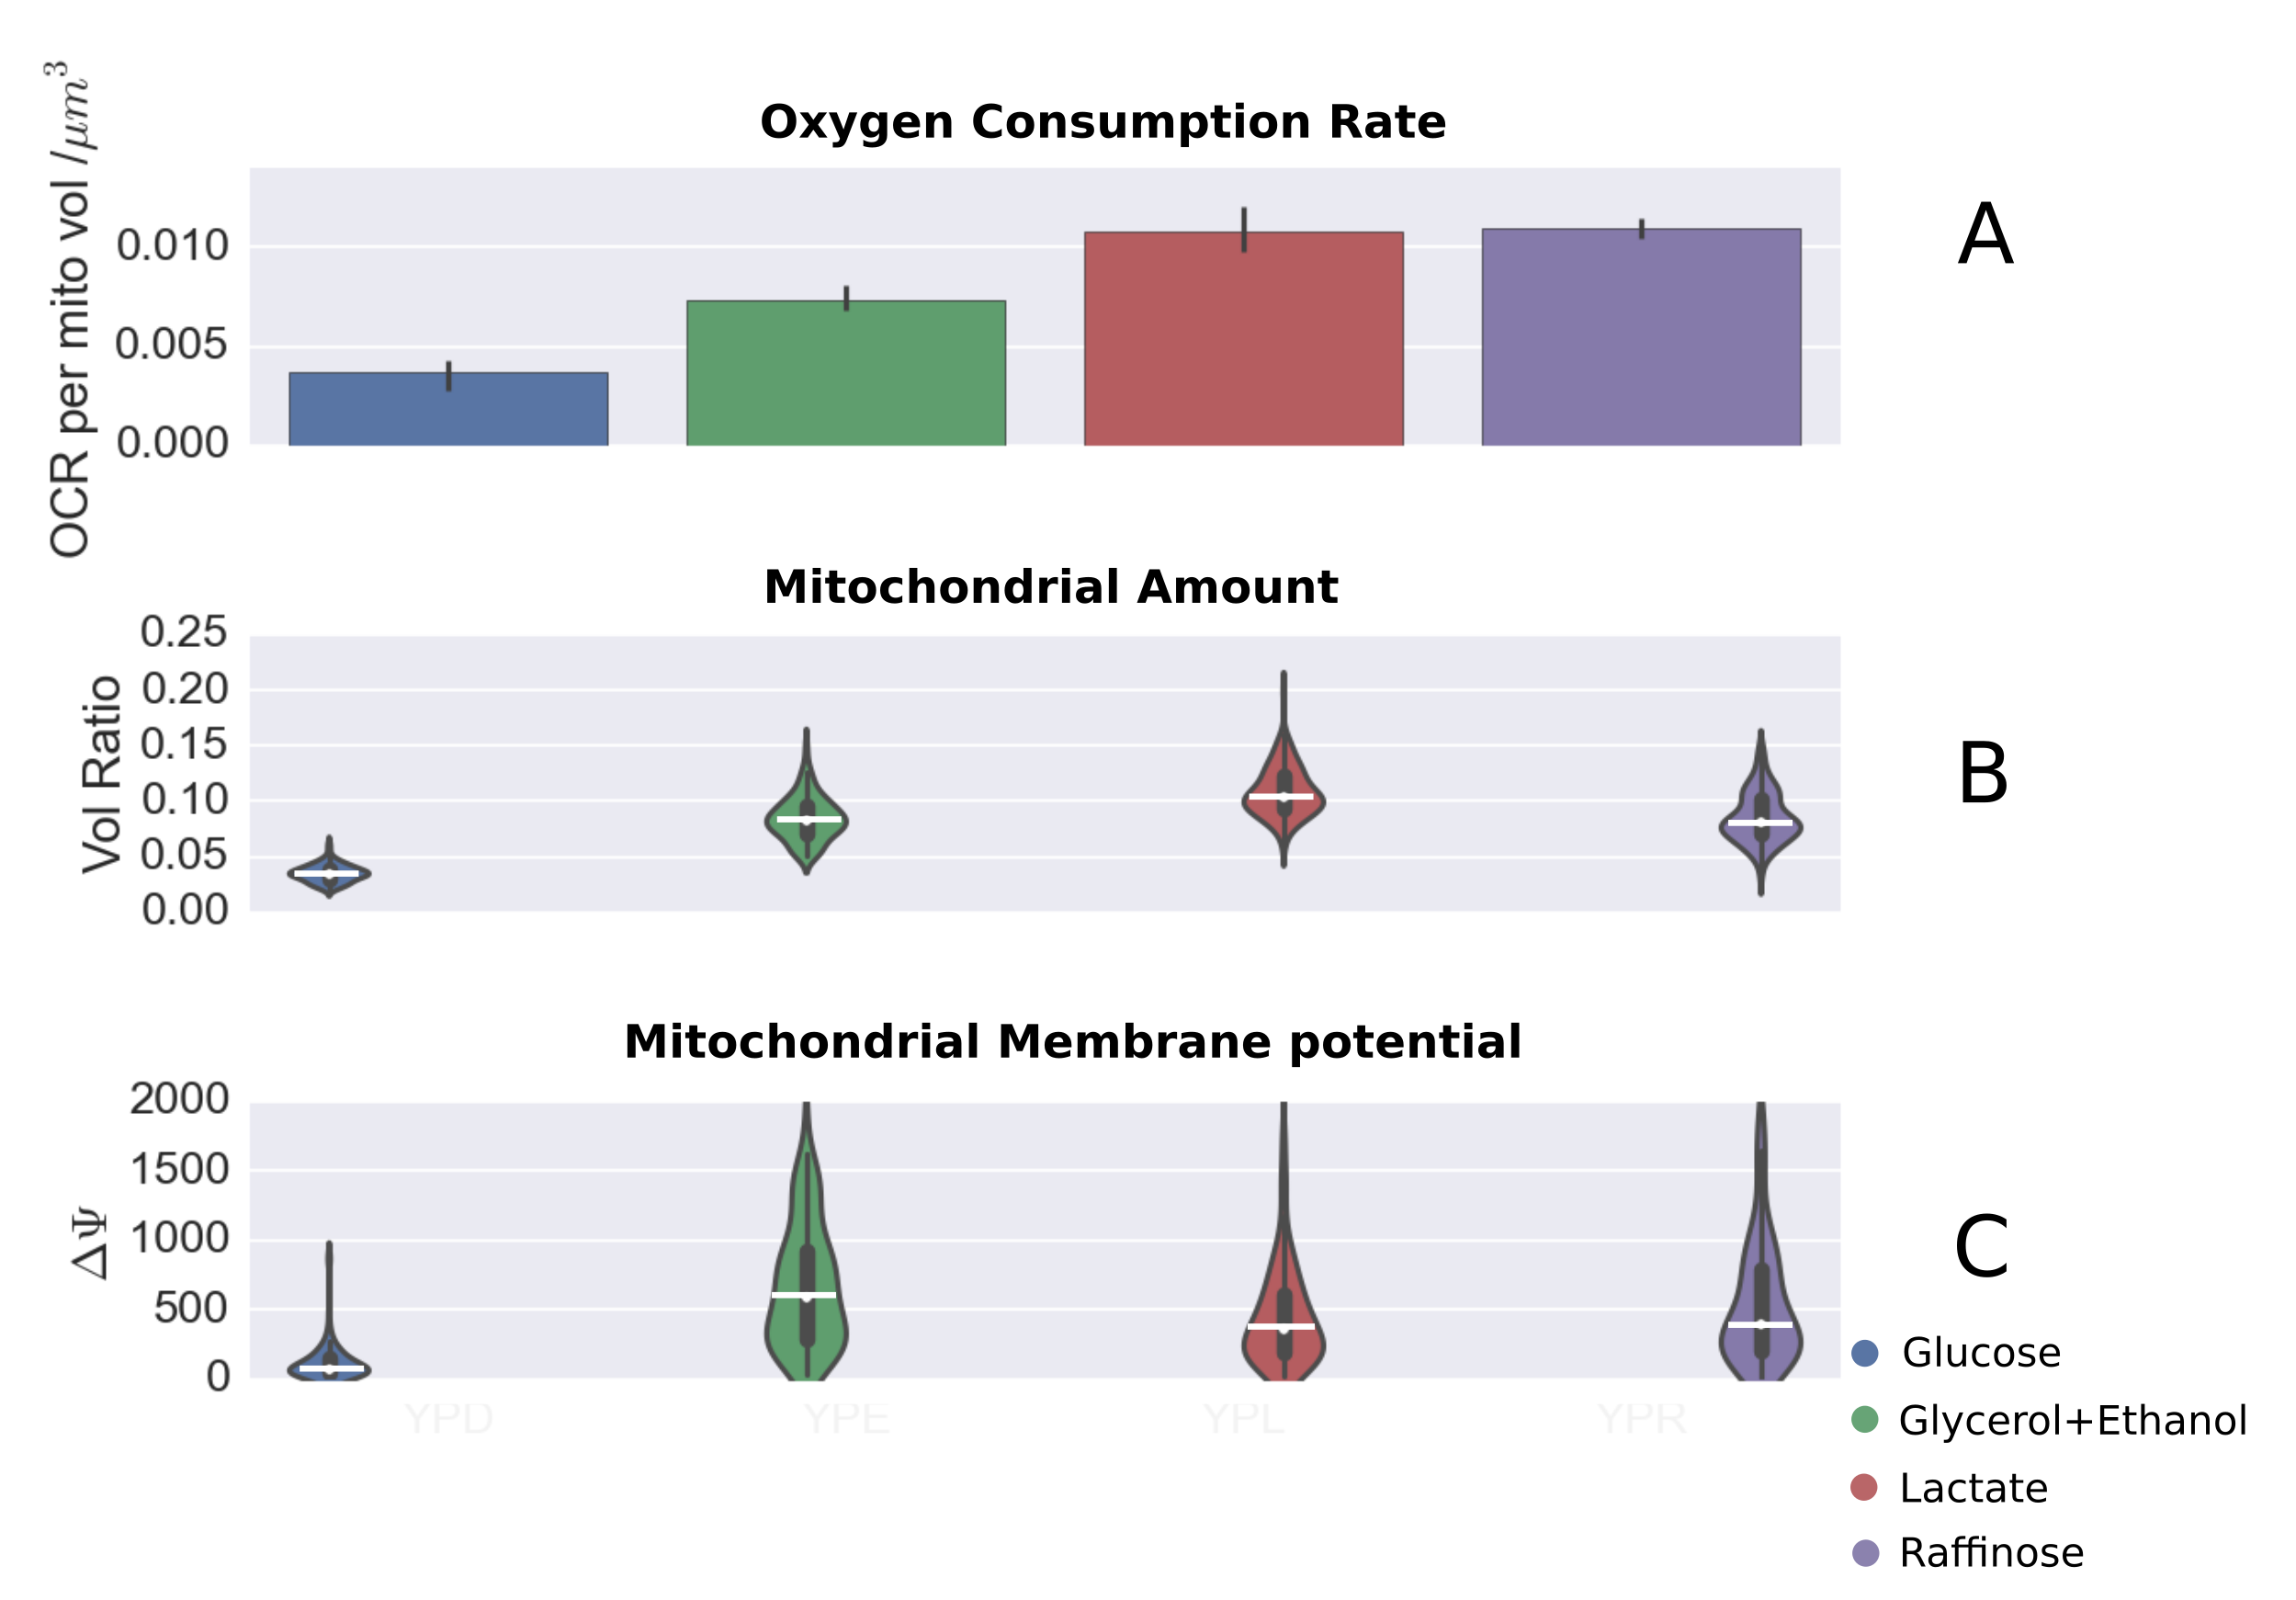
\includegraphics[width=\textwidth]{o2dy}
       \subcaptionbox{OCR normalized by mitochondrial volume\label{fig:O2dyA}}[\linewidth]{}
      \subcaptionbox{Mean volume ratio of population\label{fig:O2dyB}}[\linewidth]{}
       \subcaptionbox{Mean ΔΨ of population\label{fig:O2dyC}}[\linewidth]{}
    \caption[Relationship between mitochondrial OCR, membrane potential (ΔΨ) and amount density (volume ratio) of yeast grown in different carbon sources.]{The relationship between mitochondrial OCR, membrane potential (ΔΨ) and amount density (vol ratio) of yeast grown in different carbon sources.\\
Shown here is the relationship between mitochondrial OCR (A) and its relationship with the amount density of mitochondria in the cell (volume ratio, B) and ΔΨ (C). Mitochondria from cells grown in glycerol+ethanol display the highest ΔΨ levels and an intermediate respiration level, while those from cells grown in lactate display and intermediate level of ΔΨ and the highest respiration rate. We believe our results is due to lactate been oxidized less efficiently by the mitochondrial respiration machinery, hence the mitochondrial amount is increased in lactate to  compensate for a lesser cellular respiration efficiency. Raffinose displays similar levels of ΔΨ and respiration rates with lactate, while displaying a lower volume ratio of mitochondria. We believe that cellular respiration in raffinose is also less efficient that in glycerol+ethanol, but is able to maintain growth fitness by also undergoing fermentation.\\\emph{Error bars indicate the bootstrapped 95\% confidence interval of the median OCR value.\\White bars indicate median values.}}\label{fig:O2dy}
\end{figure}
%
\section{Discussion}
The literature has sparse references for basal OCR rate fold differences between yeast cells grown in different carbon sources under aerobic, exponential growth. Most studies used only one type of carbon condition (glucose) and therefore oxygen consumption rates are readily available for yeast grown in glucose \cite{meyenburg_energetics_1969}. One study measured the amount of basal respiration change as the amount of ethanol was slowly increased in yeast cells grown in glucose. They reported that respiration rate increased 50\% when ethanol concentration was at 2.5\%. However this was done on stationary phase (non proliferating) cells. Another study measured yeast grown in glucose repressing concentrations (2\%) and non respiration repressing concentrations (0.5\%) and found that respiration was increased two fold \cite{lin_calorie_2002}. No direct numbers could be found for basal OCR of yeast cells grown in glycerol, most likely because most often glycerol was considered as a byproduct of yeast metabolism rather than as a substrate in traditional yeast bioenergetic studies \cite{gancedo_glycerol_1968,wills_regulation_1990}. However according to one reference \cite{christopher_wills_effect_1984} only 10\% of the glycerol content is used by yeast grown on glycerol+ethanol. 

One study using lactate limited concentrations (0.2\%) reported OCR normalized to dry mass levels less than half of our results \cite{dejean_growth_2000}, but we caution that this result is not directly comparable as their growth media was substrate limiting, used a synthetic yeast nitrogen media without amino acids and had slower growth rate (doubling time 4 hrs vs 3.1 hrs). Lactate is oxidized to pyruvate by a \emph{lactate:cytochrome c} oxidoreductase complex and donates its electrons directly to cytochrome c, at the terminal end of the ETC. It has been reported that this serves as a shunt \cite{pajot_utilization_1974}, bypassing complex I, II and III. Thus because of the low proton motive force generated, one molecule of lactate only generates one ATP equivalent and hence lactate is a poor carbon source. Furthermore due to the fact that pyruvate oxidation can occur in the cytosol in yeast via the pyruvate dehydrogenase bypass \cite{boubekeur_mitochondrial_1999}, ATP yield is further reduced. Indeed it is known that the ATP/oxygen ratio of lactate is up to 50\% less than ethanol \cite{ohnishi_preparation_1966}. The high respiration reported here could be an indication that respiration is upregulated to make up for this poor ATP/oxygen ratio (known as coupling efficiency). Evidence for this is that in the previously mentioned study which used substrate limited concentrations of lactate (0.2\%), respiration rates were much less than our non substrate limited concentrations (2.0\%). However mitochondrial density is much higher than in glycerol+ethanol (\Fref{fig:O2dyB}), perhaps suggesting a compensatory upregulation of mitochondrial biogenesis to meet metabolic demands. Our growth rates for glycerol+ethanol and lactate are comparable (\textasciitilde2.9 hours for glycerol+ethanol vs 3.1 hrs for lactate, refer to growth curves in \Fref{fig:grwtcvs}), so there is evidence that cells grown in lactate have similar growth fitness with glycerol+ethanol even though lactate is a less efficient fuel source.

One study showed basal OCR levels around three fold higher in raffinose compared to glucose \cite{guaragnella_yeast_2013}, which is in good agreement with out results. However it is rather puzzling why raffinose which is considered to be able to undergo fermentation and respiration simultaneously would have a higher basal respiration rate compared to the non-fermentable carbon substrate glycerol+ethanol. One possibility is that high respiration levels seen in raffinose compared to glycerol+ethanol is due to high uncoupled respiration levels, which is further supported by the lower ΔΨ levels seen in raffinose compared to glycerol+ethanol (\Fref{fig:O2dyC}).

The best way to check whether respiration is less efficient in raffinose and lactate compared to in glycerol+ethanol is to measure respiratory control ratio (RCR). RCR is the ratio of the respiration levels at state 3 to state 4. A high RCR indicates a high level of respiration capacity with a low level of proton leak. Another similar parameter is the spare respiratory capacity, which is the difference between state 3 and basal respiration rate. This parameter indicates the capacity of the mitochondria to respond to an increase in energy demand. RCR is a complex function that depends on numerous factors such as the substrate given. Based on our hypothesis that mitochondrial respiration is less efficient in lactate and raffinose compared to glycerol+ethanol, we expect RCR values to be lower as well.

Measurement of RCR in yeast cells is problematic due to having to permeate the cell wall prior to addition of ETC chain inhibitors to achieve state 3 and 4 \cite{palmeira_fluorescence_2012}. Measurement of RCR using the Clark electrode is also difficult because the ability to add inhibitors to the sample during a measurement run is limited and multiple parallel experiments have to be conducted to obtain RCR parameters. We propose the use of the Seahorse system \cite{gerencser_quantitative_2009} to measure RCR. This system uses a piston to reversibly enclose a small volume (\textasciitilde \SI{2}{\ul}) above the cell layer. A probe containing a fluorophore is inserted into the chamber and measures the oxygen concentration by quenching of the fluorophore. The piston is then raised to allow the bulk media to reequilibrate. This system offers a convenient way to measure all the parameters related to cell respiration in one run, as up to four additions of inhibitors can be made per run.

Another possible reason that raffinose show lower respiration efficiency is that it might be somehow substrate limited. Certain common yeast lab strains lack the enzyme to metabolize melibiose, which is the form of glucose+galactose found in raffinose. However we found that our lab strain grew normally in melibiose (image data shown in \Fref{fig:meli}), therefore the yeast cells we used grown in raffinose were not substrate limited.
\chapter{Membrane potential heterogeneity at the mitochondrial tubule level}\label{ch:four}
\clearpage
\section{Introduction}
Mitochondria are double membrane organelles consisting of an outer membrane and an inner membrane. The inner mitochondrial membrane (IMM) is impermeable to most ions and metabolites. There are two distinct regions of the inner membrane \cite{vogel_dynamic_2006}, the inner boundary membrane and the cristae membrane (\Fref{fig:tubeultra}). The cristae membrane forms invaginations into the matrix and represents the majority of the surface area of the IMM. Electron transport chain (ETC) and oxidative phosphorylation (OXPHOS) proteins are concentrated in the cristae \cite{benard_ultrastructure_2008}. This enrichment in the cristae is thought to mediate efficient synthesis of ATP \cite{frey_insight_2002}.

Advances in imaging techniques in the last decade have enabled research into the changes in the IMM structure in relation to the bioenergetic and disease state of the mitochondria. Mitochondria in State 3 (high respiration, ATP synthesis activity) have increased number and size of cristae compared to mitochondria in State 4 (low respiration, no ATP synthesis). Abnormal cristae morphology is observed in mitochondrial diseases such as Leber hereditary optic neuropathy (LHON) \cite{burte_disturbed_2015} and neurodegenerative diseases such as Huntington's and Parkinson's disease \cite{yu_mutant_2003,sharma_neuroprotective_2003}. 
%
\begin{figure}[htp]
	\centering
    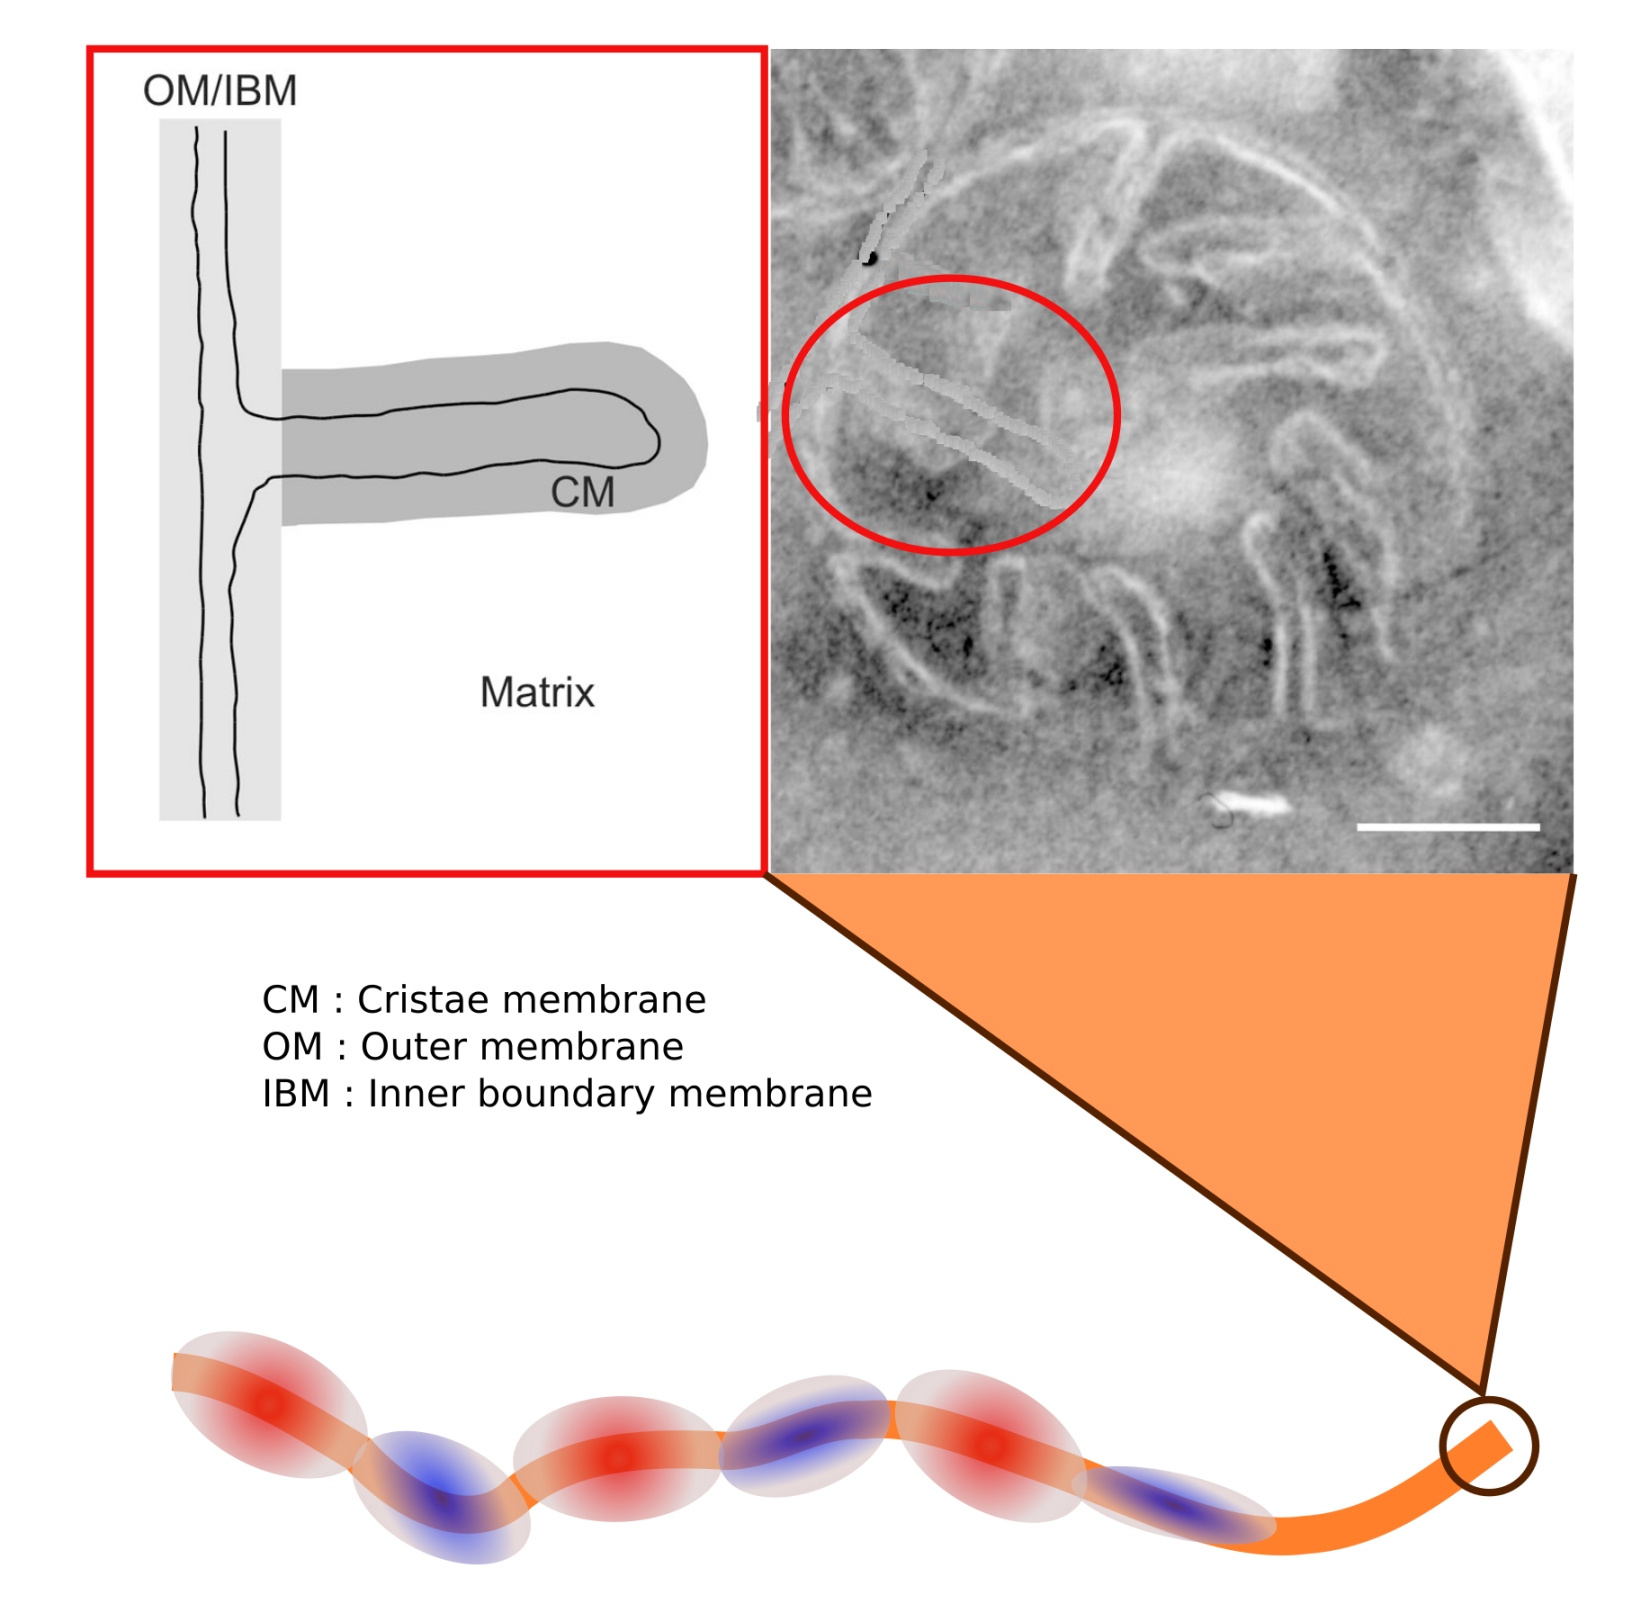
\includegraphics[width=\textwidth]{tubeultra}
    \caption[Inner mitochondrial membrane structure contributes to ΔΨ heterogeneity]{Inner mitochondrial membrane structure contributes to ΔΨ heterogeneity.\\Shown in this figure is a mitochondrial tubule displaying ΔΨ heterogeneity (higher ΔΨ levels in red, lower ΔΨ in blue). A transmission electron microscope (TEM) cross section of a real yeast mitochondrial tubule is shown in the top right image. The image was from a chemically fixed, immuno gold labeled cryosection of yeast grown in 2\% lactate. The double membrane structure of the mitochondria is visible (white edges) and the ultrastructure detail of a cristae region is shown in the top left image. Scale bar: 100 nm\\\emph{TEM images adapted from Figure 1 of Vogel et al., "Dynamic subcompartmentalization of the mitochondrial inner membrane", J Cell Biol 2006, doi:10.1083/jcb.200605138}}\label{fig:tubeultra}
\end{figure}
%

The quality and bioenergetic state of mitochondria is intimately linked to mitochondrial membrane potential (ΔΨ). The electric potential generated across the inner membrane by ΔΨ provides the energy potential to drive ATP synthesis, as well as playing a role in ROS production, mitochondrial fusion dynamics \cite{twig_mitochondrial_2008} and mitochondrial biogenesis via protein import. It has been proposed that cristae can effectively create a high resistance narrowing of the matrix lumen, effectively compartmentalizing the mitochondria into electrically distinct regions \cite{frey_insight_2002}. This would make it possible to observe heterogeneous distributions of ΔΨ within a single mitochondrial tubule due to this electrical compartmentalization by the cristae. This is thought to benefit ATP synthesis by providing a local region of high proton motive force near the cristae membrane \cite{song_biophysical_2013}, where the majority of the OXPHOS proteins are located. Whether ΔΨ can actually form heterogeneous distributions in a single mitochondrial unit is an active research field \cite{collins_mitochondria_2002,kuznetsov_heterogeneity_2009,twig_tagging_2006} because of the significance of the relationship between mitochondrial network structure and function in health and disease \cite{twig_tagging_2006}.  The following is a brief summary of previous studies on the distribution of ΔΨ within a mitochondrial tubule.

One study claimed that the ΔΨ field is equipotential across a single mitochondrial network \cite{amchenkova_coupling_1988}. They showed this by laser photobleaching a small area of the network and observed that the rest of the network promptly depolarized. Other studies found that staining with JC-1 (a ratiometric membrane potential dependent dye) resulted in significant voltage gradients along a single mitochondrial tubule \cite{bereiter1999single,smiley_intracellular_1991}. Neither studies are conclusive because firstly a diffuse depolarization of ΔΨ on local damage does not necessarily imply a homogeneous distribution of ΔΨ, while the JC-1 dye has been known to display aggregation artifacts.

One study provided evidence for the existence of discrete domains of ATP synthase cluster located at the inner membrane invaginations \cite{jimenez_mitochondrial_2014}. It is not hard to imagine that there might exist a local concentration of ΔΨ where these ATP clusters are located. One of the very first studies on ΔΨ heterogeneity within a single mitochondrial segment used human fibroblasts and astrocyte cells stained with a Nernstian membrane potential dye, TMRM \cite{diaz_homogeneous_2000}. They picked several distinct segments of mitochondria from a single cell and plotted the distributions of the ΔΨ within each mitochondrial segment. They found that the inter-mitochondrial ΔΨ variance was much higher than the variance within a single mitochondrial segment, and based on this result concluded that the ΔΨ distribution was homogeneous within a single segment. However it is not clear that all of the individual mitochondrial segments picked were really distinct units, because mitochondria in mammalian cells tend to pile up and are difficult to separate out even by eye. Indeed their own data showed that for several mitochondrial segments adjacent to each other, the variation in ΔΨ was high between these segments.

The difficulty in establishing a consistent pattern of heterogeneity is due in part to a lack of using the proper quantitative tools to establish a baseline 'control' distribution of ΔΨ within a mitochondrial tubule. Without a baseline the previous studies could not conclusively state what is a homogeneous or heterogenous distribution of ΔΨ.  Here we present an investigation into the distributions of ΔΨ in mitochondrial tubules using standard signal processing techniques (autocorrelation, spectral analysis etc). We show evidence for the existence of nonrandom heterogeneity of ΔΨ within a single mitochondrial tubule. We also investigated the distribution of ΔΨ in mitochondria growing in different respiratory states and found a statistically significant difference in their spatial frequency content.
\section{Materials and Methods}\label{sec:mmch4}
Cell growth conditions, preparation and imaging methods were carried out as in \fref{sec:MM2}. The cells were grown in four different carbon sources as detailed in \fref{sec:carbon}. The number of cells N in each carbon source were---glucose (N=96), glycerol+ethanol (N=111), lactate (N=117) and raffinose (N=96).
%
\begin{figure}[htp]
	\centering
    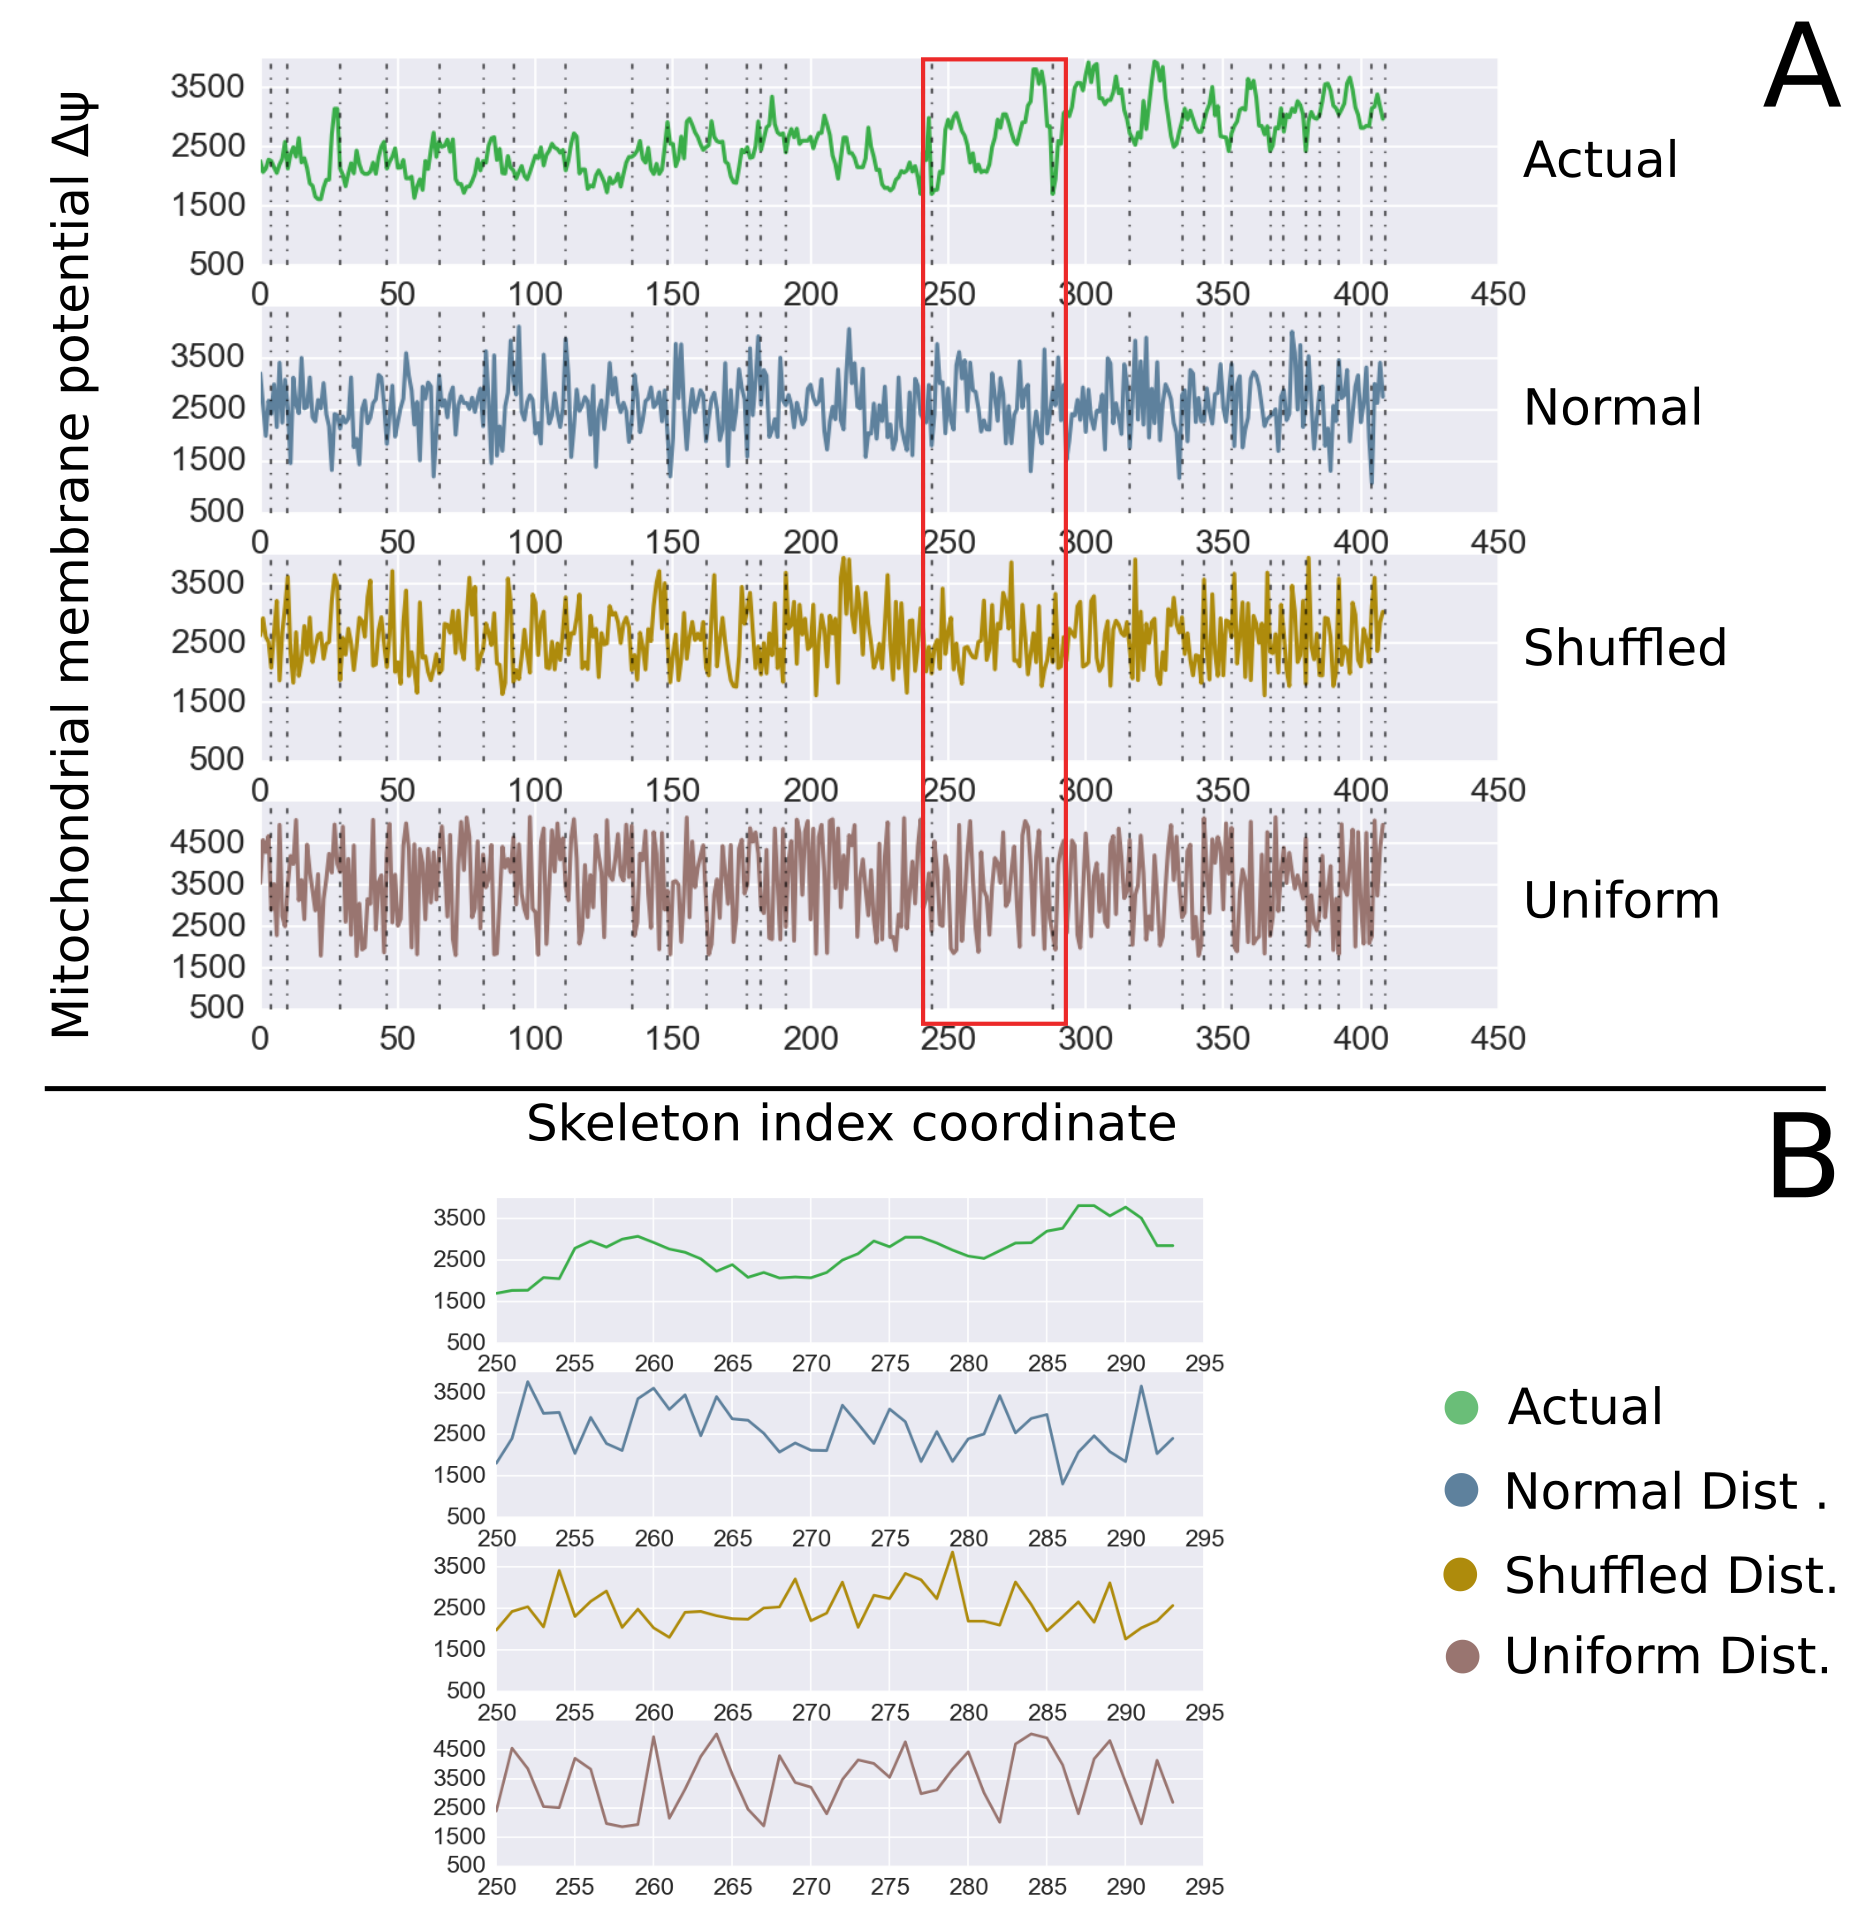
\includegraphics[width=.95\textwidth]{random}
    \subcaptionbox{ΔΨ distribution in all tubules from a single cell. The x-axis represents a coordinate system where all the tubules in that cell are lined up end to end. The vertical dotted lines indicate the boundaries of a tubule within that cell. The red box highlights a single tubule and is shown in more detail in the \Fref{fig:randomB}.\label{fig:randomA}}[\linewidth]{}
    \subcaptionbox{ΔΨ distribution in a single tubule from the same cell (highlighted by the red box in \Fref{fig:randomA}). \label{fig:randomB}}[\linewidth]{}
    \caption[Tubule level ΔΨ heterogeneity in actual and random distributions]{Tubule level ΔΨ heterogeneity in actual and random distributions.\\Mitochondrial membrane potential (ΔΨ) distribution in tubules are plotted and compared with fitted random distributions. The three random distributions below the 'Actual' distribution represent baseline levels of mitochondrial ΔΨ homogeneously distributed with random variations due to optical and experimental conditions. Actual distributions of ΔΨ display much smaller variation in ΔΨ between adjacent pixels.
}\label{fig:random}
\end{figure}
%
\subsection{Sampling of random distributions}
The random distributions shown in (\Fref{fig:random}) were obtained as follows:
For each cell, let the mitochondrial network with a total of $N$ pixels be a vector of signal intensities $\{X_0, X_1 \cdots X_{N-1}\}$, where the subscripts indicate the order indices of the pixels. The signal intensities represent the normalized ΔΨ as described in \Fref{ch:two}. The indices represent the coordinates of the pixels along an imaginary one dimensional axis that would be obtained from lining up all the tubules in the mitochondrial network end to end.

We calculate the sample mean and variance of this set, $\mu$ and $\sigma^2$ as follows:\\
At each pixel position, we sampled from a normal distribution $N(\mu,\sigma^2)$  to get sampled intensities $\{X_{s0}, X_{s1} \cdots X_{sN-1}\}$. This is was then plotted as the 'Normal' distribution graph shown in \Fref{fig:random}. A similar procedure was used for the 'Uniform' distribution graph, where we sampled from a uniform distribution $U(\mu-1.5\sigma, \mu+1.5\sigma)$ at each pixel position. The range of the uniform distribution was chosen so as to approximate a distribution that encompassed 99.7\% of the Normal distribution range.
For the 'Shuffled' distribution graph, we randomly permuted the set of original signal intensities to get a permuted set $\{X_{p0}, X_{p1}, \cdots X_{pN-1}\}$, where for example, the signal intensity $X_{p0}$ represents the randomly shuffled signal intensity at the pixel position 0.
\subsection{Autocorrelation curves}
The autocorrelation coefficient $R(k)$ measures the 'memory' of a signal by correlating pairs of points within the signal separated by a lag distance, $k$. A high value of autocorrelation at large lag distances implies that the signal has memory at large length scales.
The autocorrelation curves for \Fref{fig:autorandom} and \Fref{fig:autoactual} were derived as follows:
For a single tubule of length $N$ with signal intensity $\{X_0, X_1 \cdots X_{N-1}\}$ the autocorrelation coefficient $R(k)$ as a function of pixel lag distance $k$, was calculated as \cite{priestley1981spectral}:
\begin{align}\label{eq:autocor}
	R(k)&=\frac{1}{(N-k)\sigma^2} \, \displaystyle\sum_{t=1}^{N-k}  (X_t-\mu )( X_{t+k}-\mu) \nonumber \\
	&\! \text{for }k_0,k_1 \cdots k_{15}
\end{align}
The terms $\mu$ and $\sigma$ are the sample mean and variance of the tubule respectively. Since we are using the sample mean and variance, the autocorrelation coefficient is a biased estimate. We restricted our tubules to a minimum length of 40 pixels to minimize the bias error from using the sample mean and variance while ensuring we had enough tubules to obtain sufficient statistical power. For the populations of tubules from the various carbon source we had a range of 144--250 tubules with this minimum length (glucose=144, glycerol+ethanol=218, lactate=230, raffinose=177). This represented 10--15\% of the total tubule population. We then averaged all the autocorrelation coefficient at a given lag distance $k$ and plotted the mean autocorrelation curve for tubules with this minimum length. Tubules from populations of cells from random distributions (\Fref{fig:autorandom}) and growing in different carbon sources (\Fref{fig:autoactual}) were plotted.
%
\begin{figure}[htp]
	\centering
    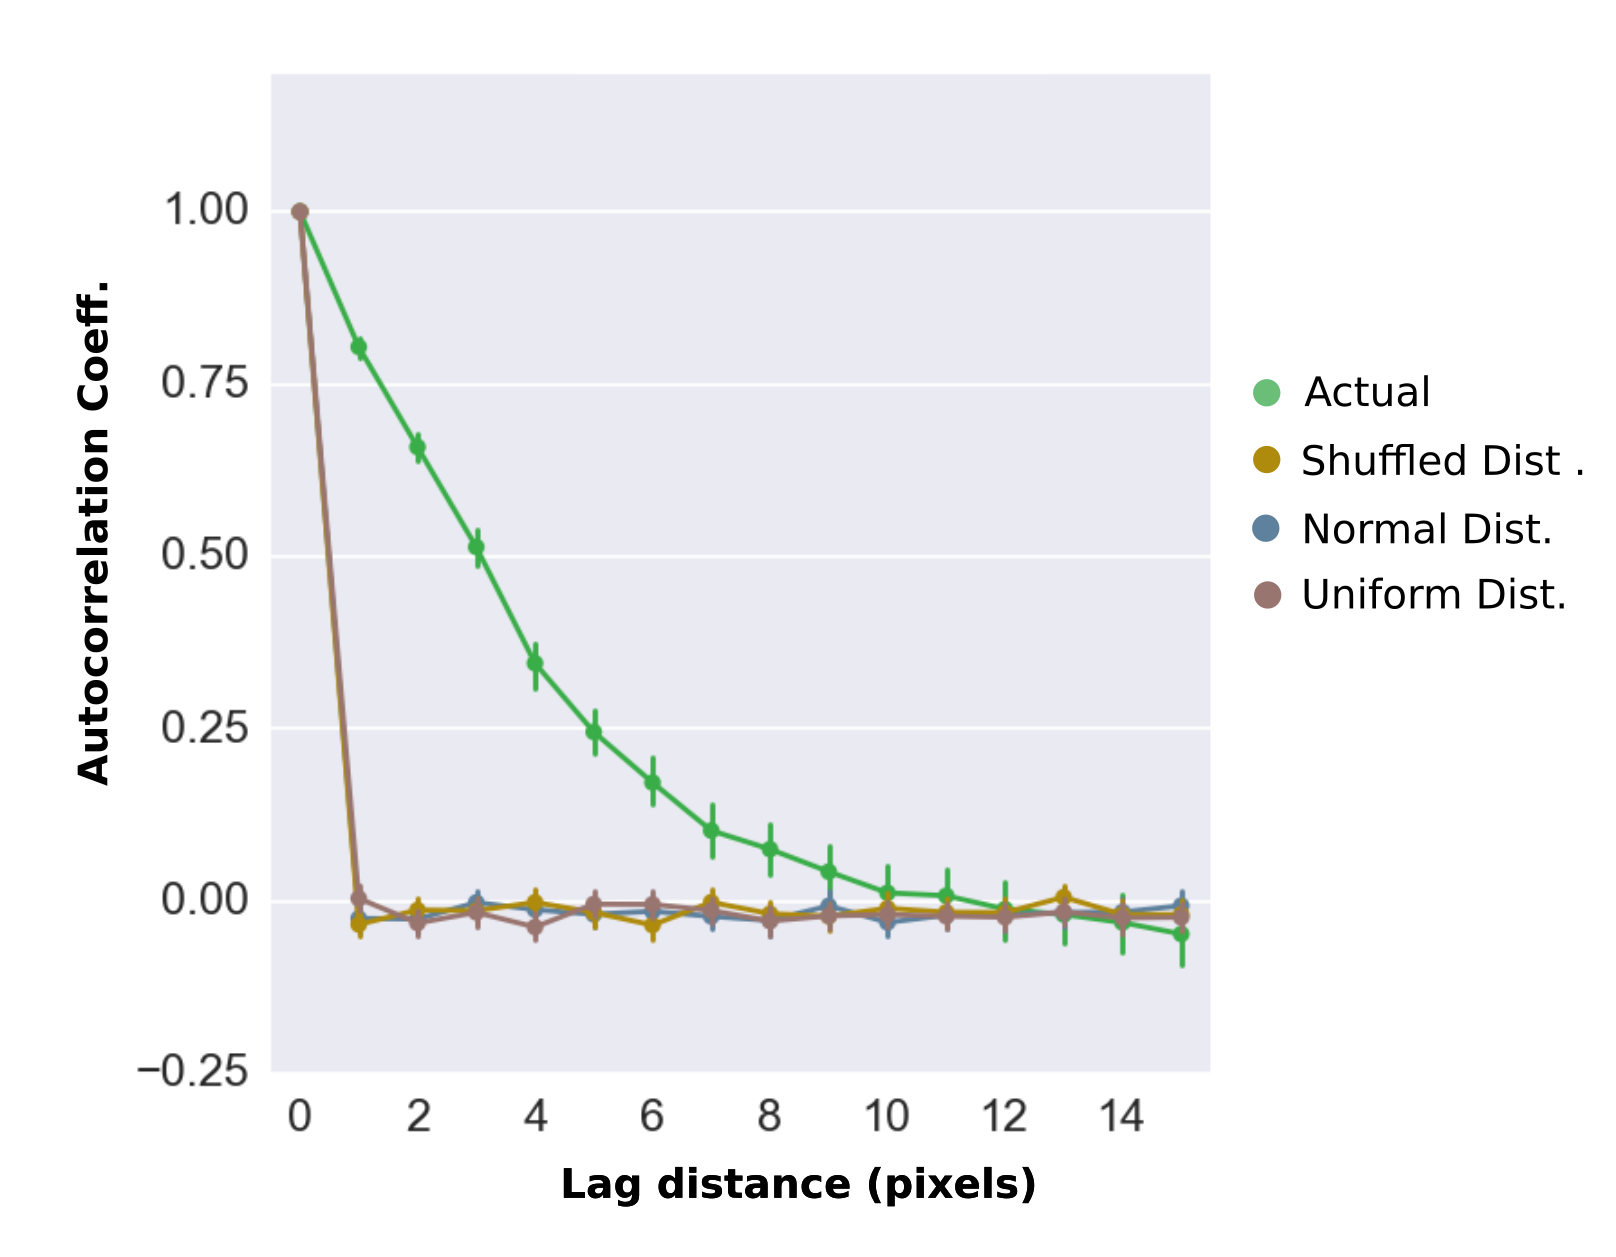
\includegraphics[width=.75\textwidth]{autorandom}
    \caption[Autocorrelation curves of actual vs random distributions]{Autocorrelation curves of actual vs random distributions.\\Shown here is the autocorrelation coefficient distribution of a real population of cells (green curve, grown in glycerol+ethanol) and three random populations. The autocorrelation of ΔΨ distribution from a real population of mitochondrial tubules displays higher autocorrelation coefficients at large length scales (lag distance) compared to random distributions.\\\emph{Error bars represent the bootstrapped 95\% confidence interval of the mean.}}\label{fig:autorandom}
\end{figure}
%
%
\begin{figure}[htp]
	\centering
    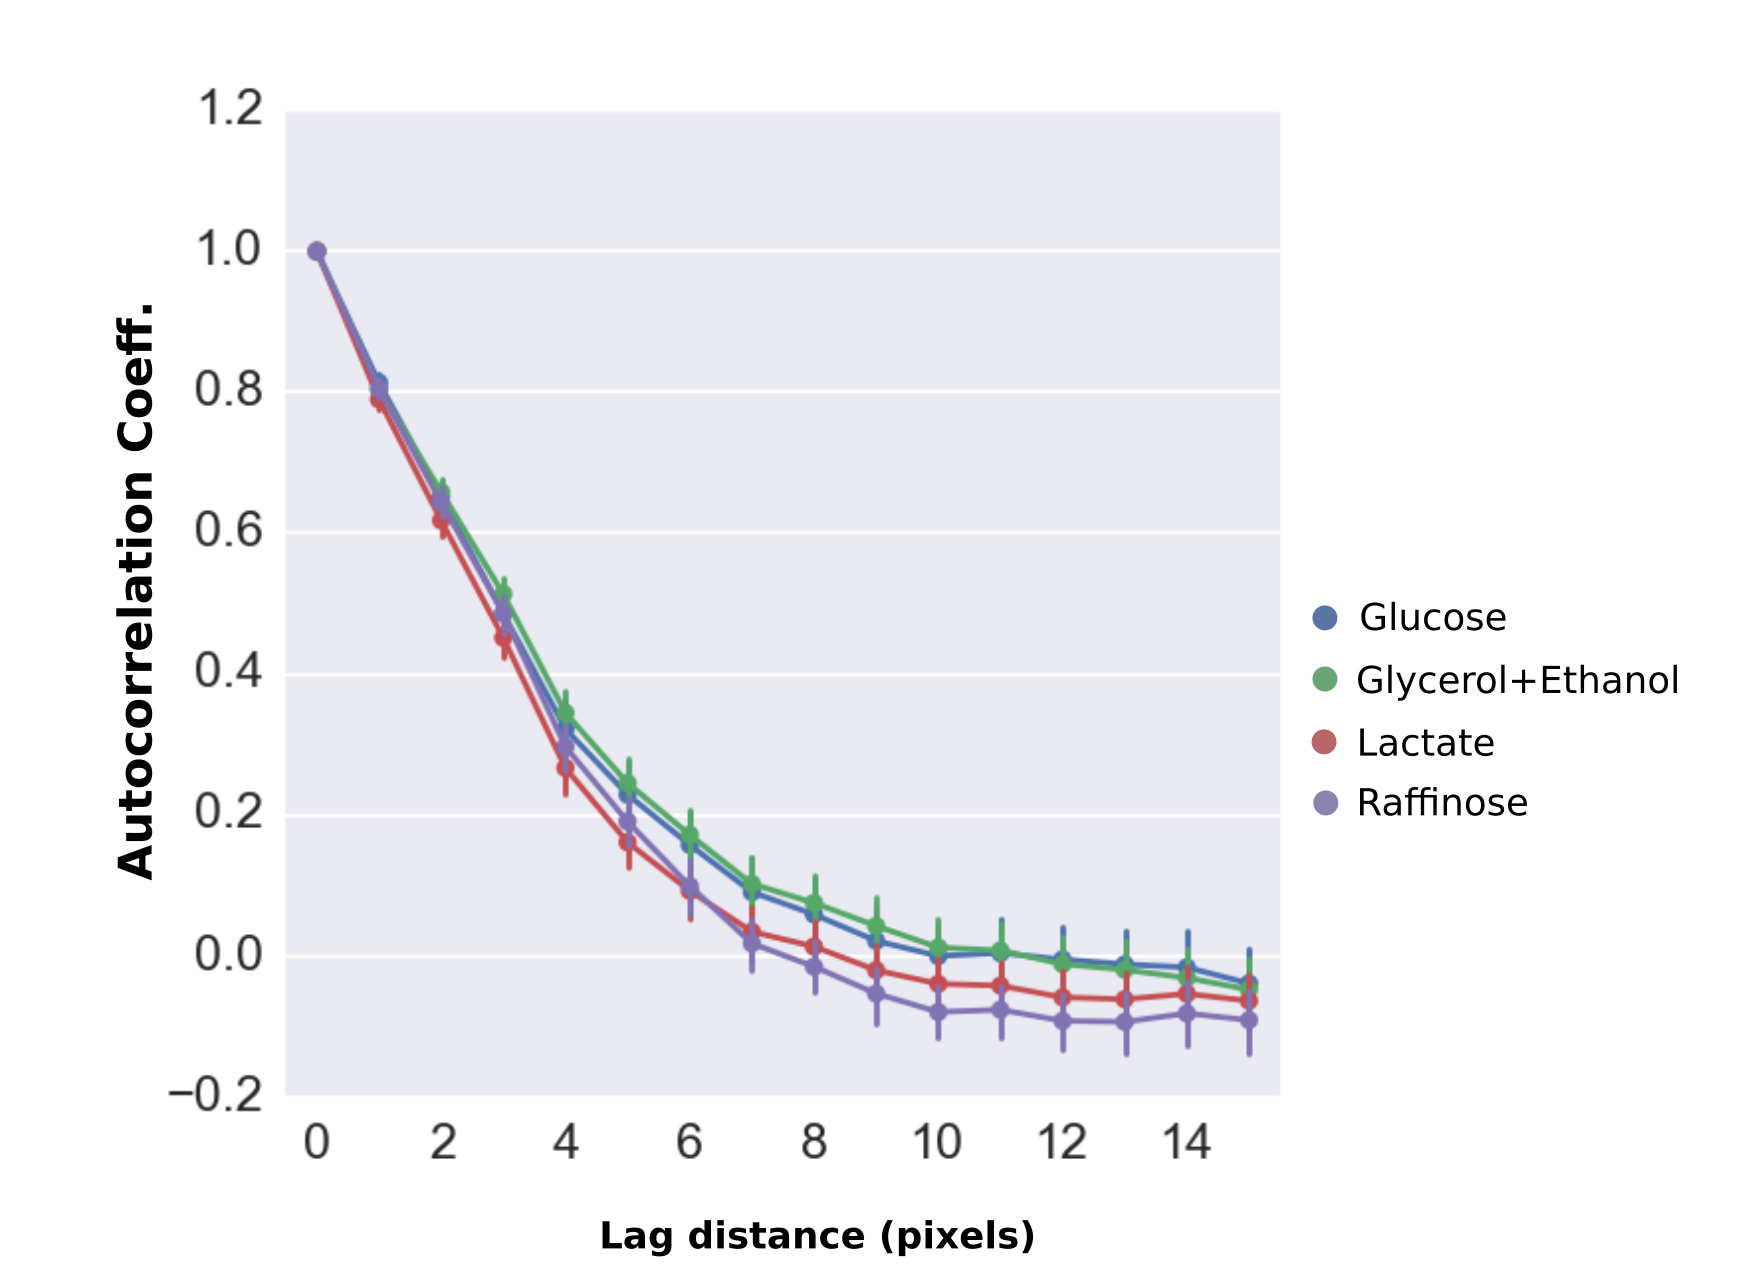
\includegraphics[width=.7\textwidth]{autoactual}
    \caption[Autocorrelation curves of populations of cells growing in different carbon sources]{Autocorrelation curves of populations of cells growing in different carbon sources .\\Shown here are the autocorrelation coefficient distributions of cells grown in either fermentation (glucose), respiration only (glycerol+ethanol, lactate) and respiration+fermentation (raffinose). Mitochondrial tubules grown in the different conditions do not show a statistical difference in their autocorrelation curves.\\\emph{Error bars represent the bootstrapped 95\% confidence interval of the mean.}}\label{fig:autoactual}
\end{figure}
%
%
\begin{figure}[htp]
	\centering
    \hspace*{.65in}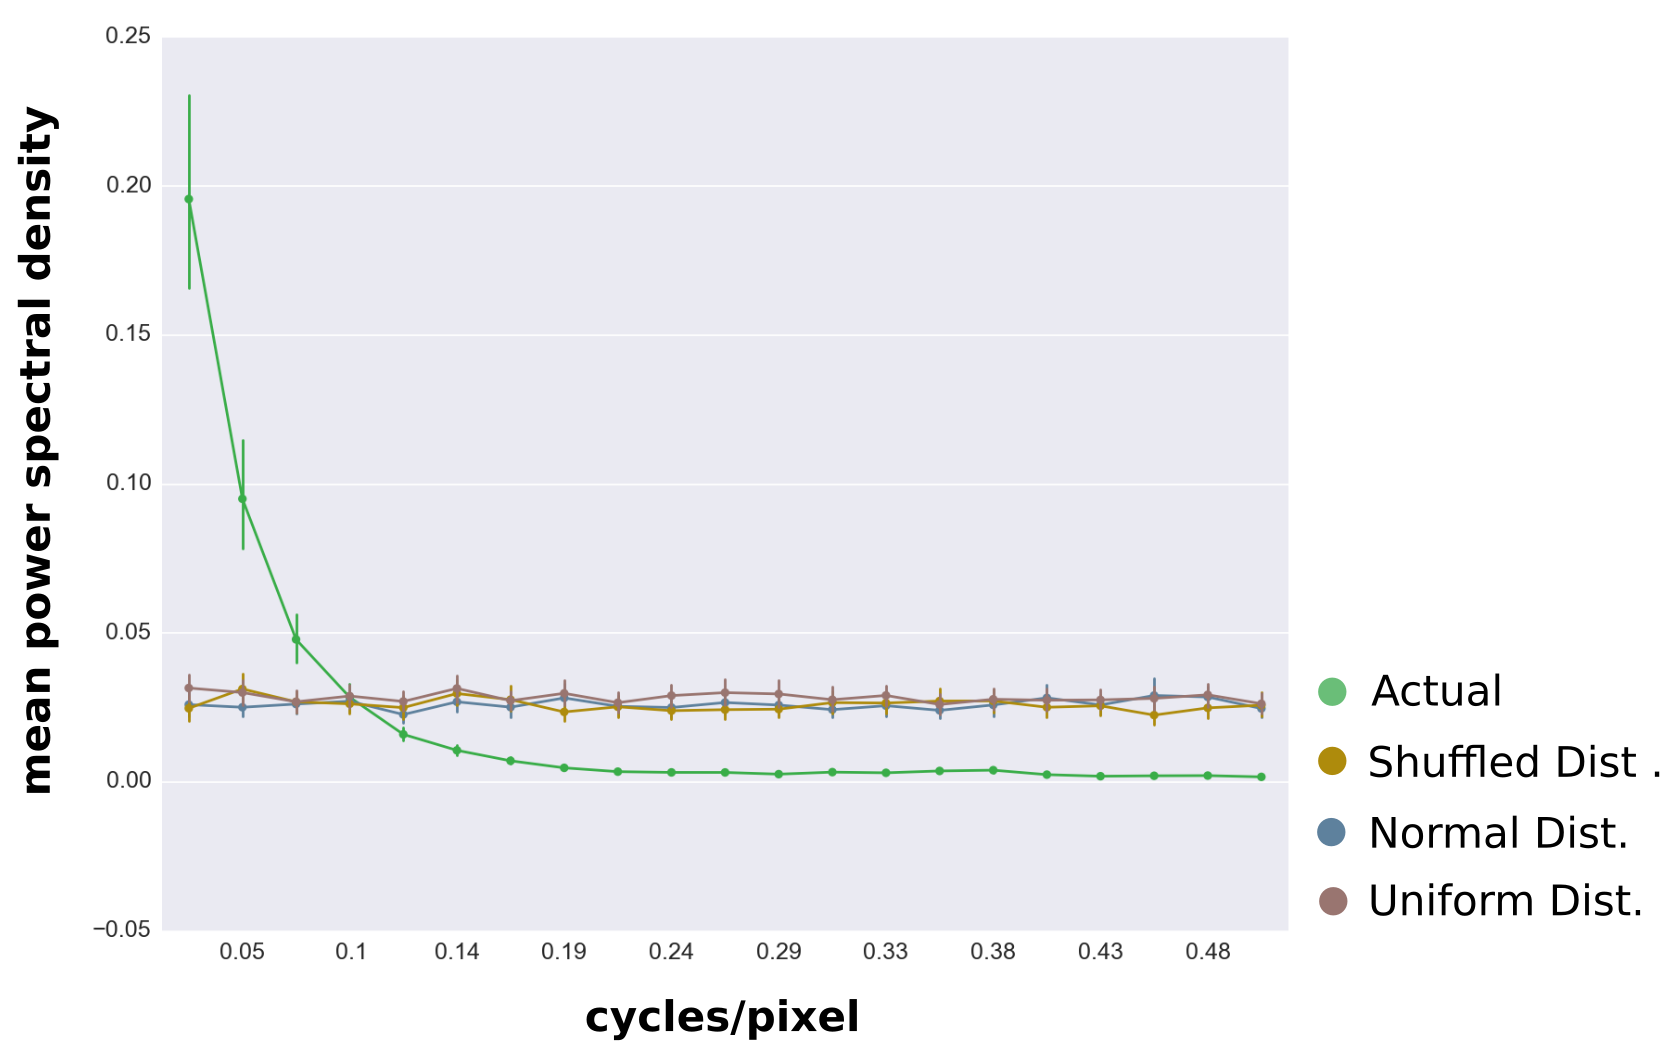
\includegraphics[width=.8\textwidth]{psdrandom}
    \caption[Power spectral density of actual vs random distributions]{Power spectral density of actual vs random distributions.\\Shown here is the power spectral density of a real population of cells (green curve, grown in glycerol+ethanol) and three random populations. The power spectral density of ΔΨ from a real population of mitochondrial tubules displays much more power at lower spatial frequencies (i.e. higher correlation at larger length scales) compared to random distributions (observe the high power on the y-axis at values of <0.1 for the x-axis compared to the random distributions).\\\emph{Error bars represent the bootstrapped 95\% confidence interval of the mean.}}\label{fig:psdrandom}
\end{figure}
%
%
\begin{figure}[htp]
	\centering
    \hspace*{.65in}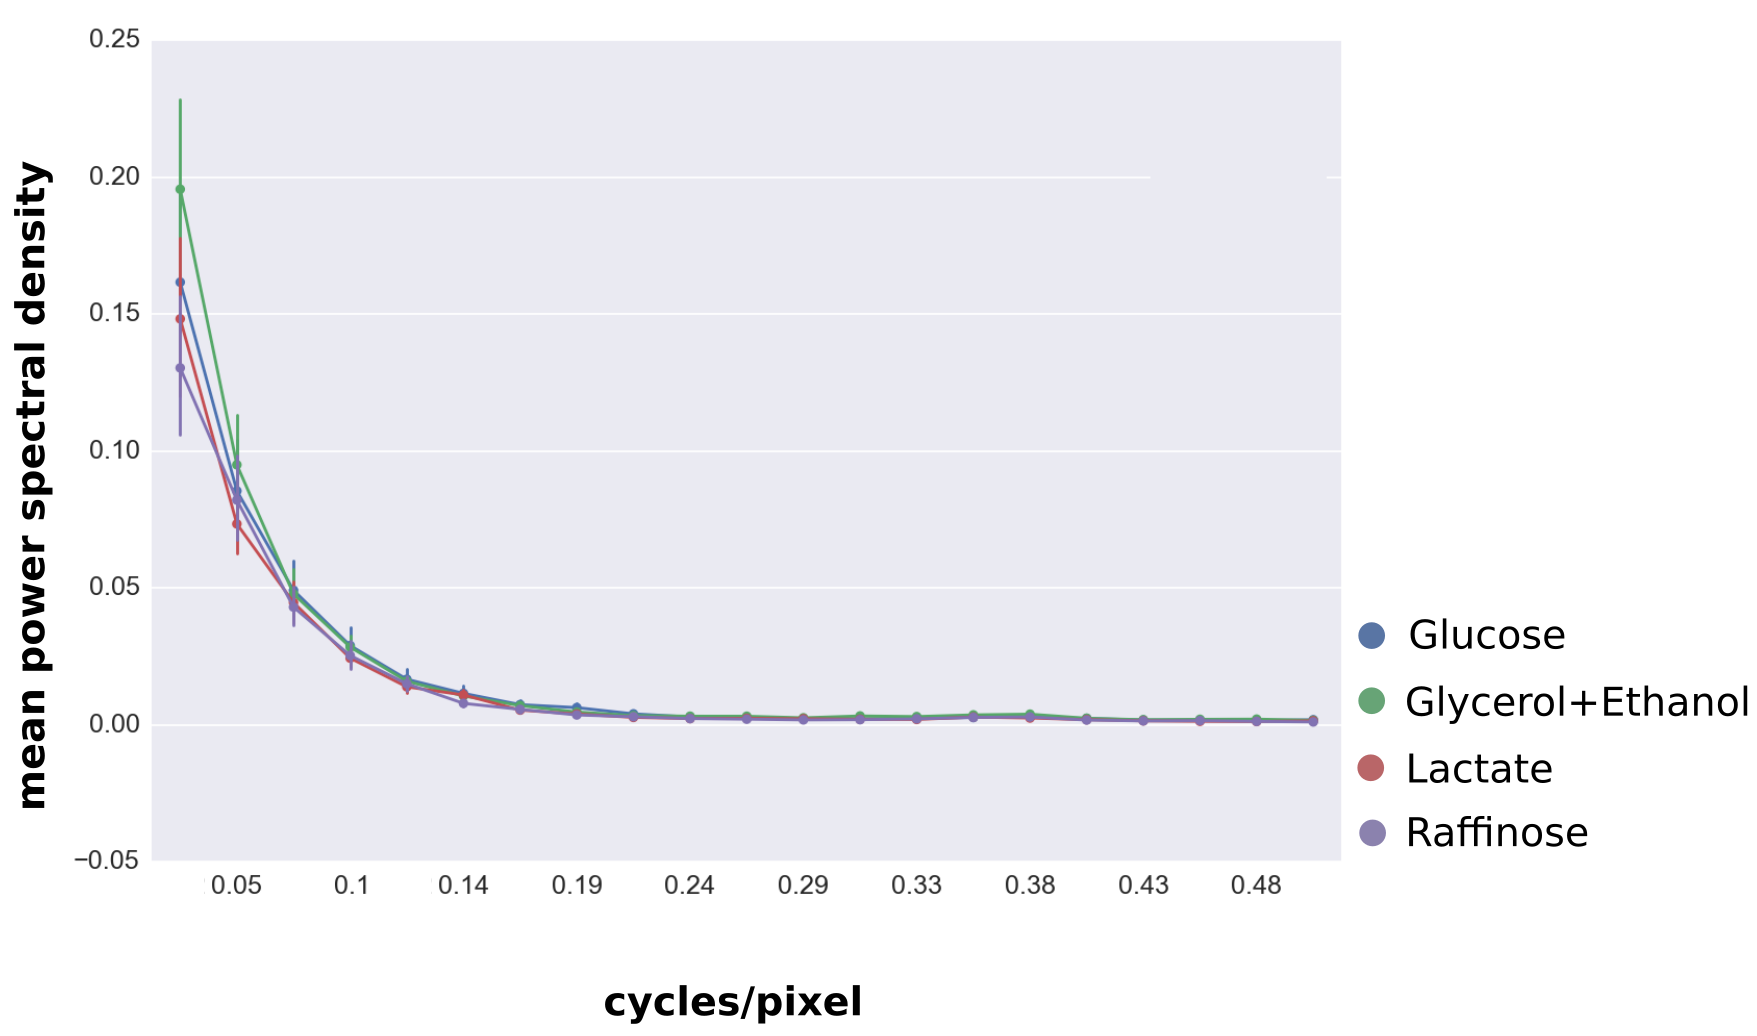
\includegraphics[width=.85\textwidth]{psdactual}
    \caption[Power spectral density of populations of cells growing in different carbon sources]{Power spectral density of populations of cells growing in different carbon sources.\\Shown here are the power spectral densities of cells grown in either fermentation (glucose), respiration only (glycerol+ethanol, lactate) and respiration+fermentation (raffinose). Mitochondrial tubules grown in respiration and fermentation (glucose) do not show a statistical difference in their spatial frequency content.\\\emph{Error bars represent the bootstrapped 95\% confidence interval of the mean.}}\label{fig:psdactual}
\end{figure}
%
\subsection{Power spectral density}
The power spectral density (PSD) is defined as the square of the modulus of the Fourier transform of a signal and is a measure of the spatial frequency content of the signal. Spatial frequency is the inverse of spatial length, a higher spatial frequency implies a smaller length scale \cite{schowengerdt_chapter_2007}. For a single tubule of length $N$ with signal intensity $\{X_0, X_1 \cdots X_{N-1}\}$ and sampling rate of $Δt=1$ pixel, the power spectral density $S(f)$ as a function of spatial frequency $f$ is estimated as the modulus squared of the discrete Fourier transform (DFT) \cite{priestley1981spectral}:
\begin{align}
	S(f)&=\frac{Δt}{N} \: \left\vert\displaystyle\sum_{t=0}^{N-1}  X_n \exp ^{-i 2 \pi nf}\right\vert^2 \nonumber \\
	&\! f\leq \frac{1}{2Δt} \; \text{for real frequencies}
\end{align}

We calculated the power spectral density using the Numpy.fft.rfft module (\url{http://www.numpy.org/}), which calculates the DFT for real input functions. Since we are limited to a sampling resolution of 1 pixel, the maximum frequency we can get will be 0.5 cycles/per pixel. Ideally $N$ should be as large as possible to get the 'true PSD', i.e. with larger $N$ we will get finer resolutions of $S(f)$. Similar to the derivation of the autocorrelation curve, we restricted our tubules population to be a minimum of length 40 pixels so that we get a minimum of 20 values of $f$ between 0--0.5 cycles/pixel. The DFT returns positive and negative frequencies; we ignore negative frequencies for real spatial values. We then averaged the function by spatial frequency $f$ and plotted the mean $S(f)$ curve for all the tubules in the population. Tubule populations of cells from random distributions and in different growth conditions were plotted (\Fref{fig:psdrandom} and \Fref{fig:psdactual}).

By the Wiener–Khinchin theorem \cite{kay1981spectrum}, the power spectral density $S(f)$ is the Fourier transform of the autocorrelation function $R(k)$:
\begin{equation}
	S(f)= \displaystyle\sum_{k=-\infty}^{\infty} R(k) \exp^{-i 2 \pi n f}
\end{equation}
Therefore we can think of the power spectral density as the frequency transformed version of the information provided by the autocorrelation curves. A power spectrum that has high power at low frequencies implies a greater correlation at large length scales. 
\subsection{Delta intensity \texorpdfstring{$ΔI(k)$}{DIk}}
One problem with using autocorrelation is that we are using a biased estimate of the autocorrelation due to using the sample mean and variance of the tubule. Therefore in order to minimize the sample bias we restricted the tubule population to a minimum length 40 pixels, but this meant we were excluding a large proportion of tubules that fell below this threshold (up to 90\% of the tubules).
Referring to \eqref{eq:autocor}, the terms inside the summation represent the covariance between points on the tubule. Instead of using the covariance, we defined another function $ΔI(k)$:
\begin{align}
	ΔI(k)&= \left\vert \displaystyle\sum_{t=1}^{N-k} X_t-X_{t+k} \right\vert \nonumber \\
	& \! \text{for }k_1,k_5,k_{10},k_{15},k_{20}
\end{align}
%
\begin{figure}[htp]
	\centering
    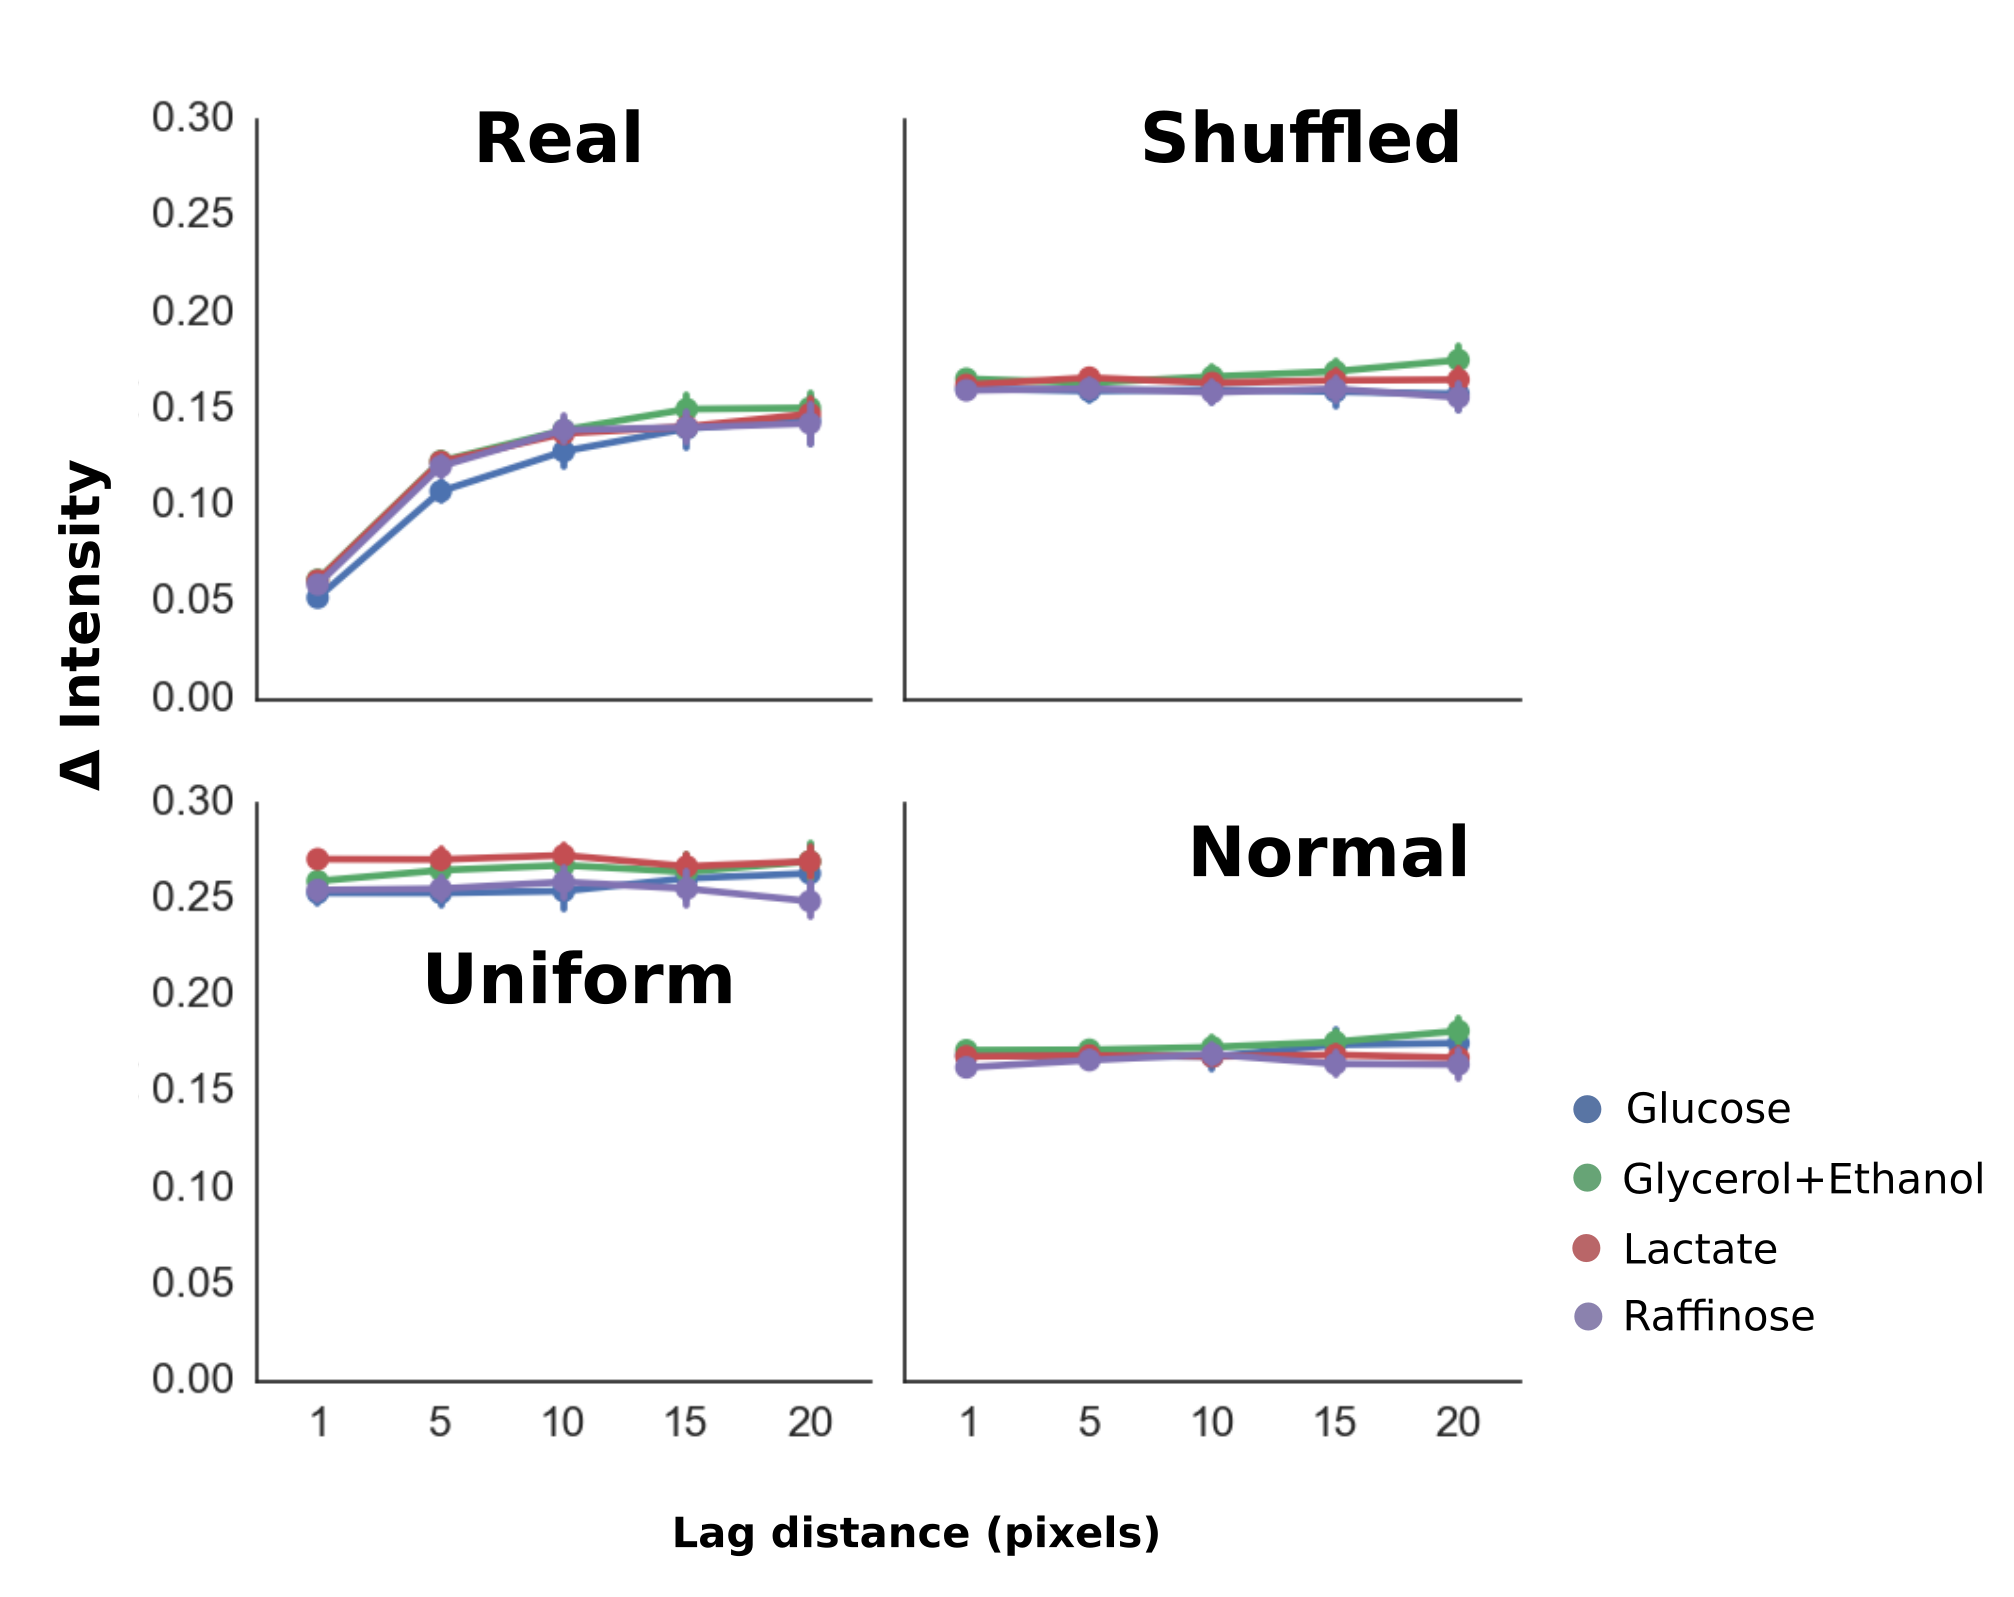
\includegraphics[width=\textwidth]{deltaI}
    \caption[Delta intensity $ΔI(k)$ curves]{Actual and random delta intensity ($ΔI(k)$) curves.\\The plot shows a panel of delta intensity $ΔI(k)$ distributions for the populations of cells grown in different carbon sources. The top left pane shows the $ΔI(k)$ of the actual populations of mitochondrial tubules grown in different carbon sources. The top right and bottom panels show the $ΔI(k)$ distribution of the random distributions (Shuffled, Uniform, Normal) plotted for each of the carbon sources. Mitochondrial tubules in all of the different carbon sources show non random distribution of $ΔI(k)$.\\\emph{Error bars represent the bootstrapped 95\% confidence interval of the mean.}}\label{fig:deltaI}
\end{figure}
%
%
\begin{figure}[htp]
	\centering
    \hspace*{.7in}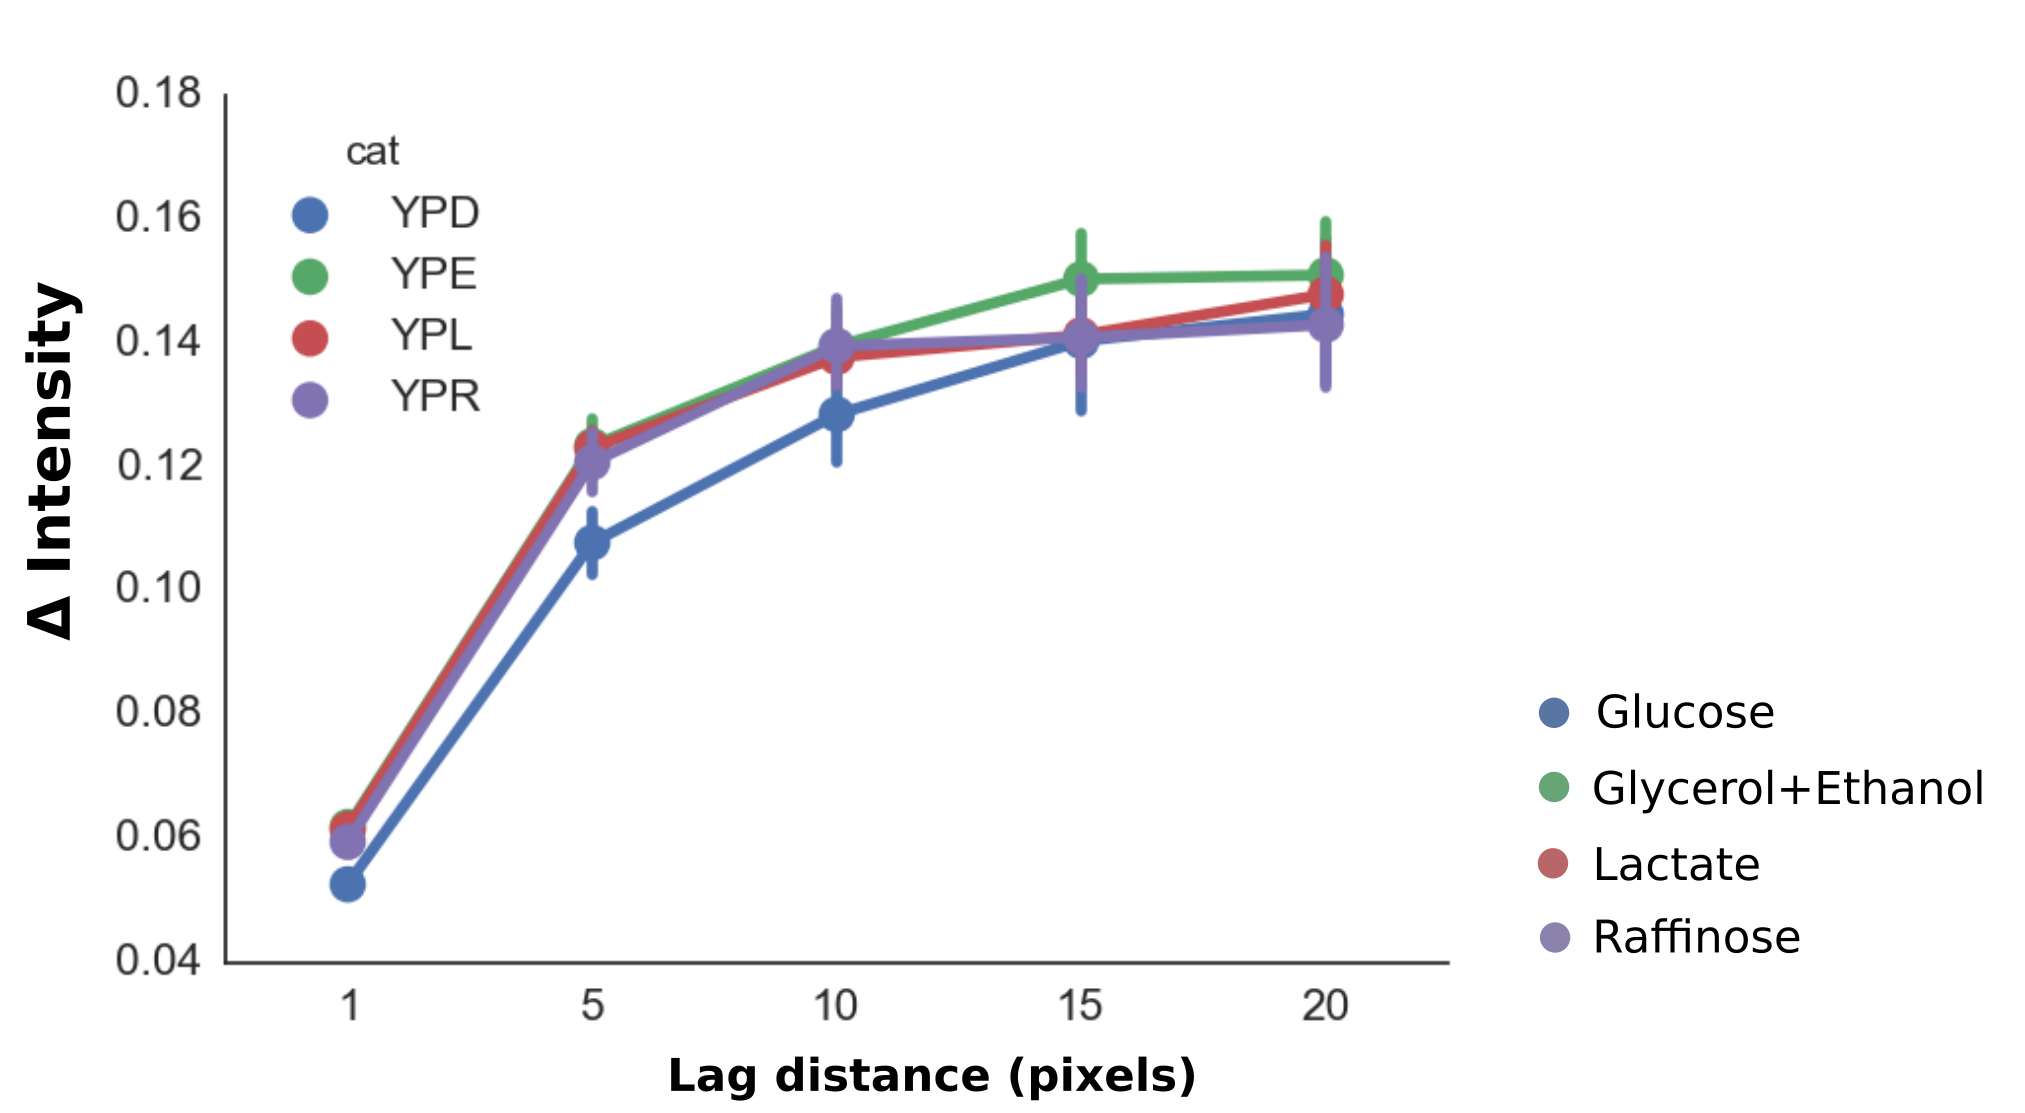
\includegraphics[width=.85\textwidth]{deltaIactual}
    \caption[$ΔI(k)$ actual for tubule populations growing in different carbon sources]{$ΔI(k)$ actual for tubule populations growing in different carbon sources.\\Mitochondrial tubules in fermentation (glucose) have lower $ΔI(k)$ at lag distances below 15 pixels, meaning that they show lower spatial frequencies and higher correlations at large length scales compared to respiratory conditions.\\\emph{Error bars represent the bootstrapped 95\% confidence interval of the mean.}}\label{fig:deltaIactual}
\end{figure}
%
This function represents the absolute difference of intensities between a pixel and another pixel separated by lag distance $k$. A large value of $ΔI(k)$ at small lag distances $k$ indicates that there is little correlation between those two pixels, and a high spatial frequency component to the signal. We averaged the function at a given lag distance $k$ and plotted the mean $ΔI(k)$ curve for all the tubules in the population. Tubule populations of cells from random distributions and in different growth conditions were plotted (\Fref{fig:deltaI} and \Fref{fig:deltaIactual}).
 
\subsection{Statistical testing with post-hoc multiple testing correction}\label{sec:stat}
In this project, whenever we made a statistical test comparing two conditions we used the ranked sum test with $p<0.05$ as the significance level to reject the null hypothesis that there was no difference between the two conditions. When performing statistical testing across multiple conditions, there is an increasing probability of making a false positive (Type I error) across all tests. This probability is known as the family wise error rate (FWER) and is given by the formula:
\begin{equation}
	\text{FWER}=1-(1-p)^n
\end{equation}
$p$ is the significance level for one comparison and $n$ is the number of comparisons. For our project, with four different carbon conditions there are six possible combinations, and at a typical significance level where we reject the null hypothesis of $p=0.05$, the FWER is \textasciitilde{27\%}. Thus it is critical that all statistical tests be corrected for multiple testing with a post-hoc correction method. We used the Holms-Sidak \cite{holm_simple_1979} multiple testing correction method which has been shown to have more statistical power \cite{seaman_new_1991} (i.e. more likely to detect an effect if the effect really existed) than the popular Tukey or Bonferonni methods while ensuring that the FWER is less than 0.05 (thus avoiding false positives due to multiple testing). The Holms-Sidak method is a recursive step-down method where the $p$ values are ranked and compared with successively larger adjusted significance levels. The method is guaranteed to control the FWER which we set at 0.05, but the disadvantage is that we cannot obtain the confidence intervals from the test. We do not require a confidence interval in our analysis for this chapter as we are only interested in whether there is a difference between the groups.

The above procedure was carried out using the StatsModels package in Python (\url{http://statsmodels.sourceforge.net/devel/generated/statsmodels.sandbox.stats.multicomp.multipletests.html}).
\section{Results}
\subsection{Mitochondrial tubules have nonrandom heterogeneity of ΔΨ}
In order to conclusively determine whether heterogeneity of ΔΨ exists within mitochondrial tubules, we must first establish a baseline to decide if a ΔΨ distribution is truly heterogeneous. We do this by comparing the distributions of the signal intensities to random distributions of ΔΨ intensities. In \Fref{fig:random} we show three different types of random distributions ('Normal, Shuffled, Uniform') below an actual distribution of ΔΨ. These three random distributions represent a 'control' or baseline level of ΔΨ homogeneously distributed with random variations due noise in the optics and experimental conditions. The Shuffled distribution is the most conservative estimate of a true random baseline as it is non parametric and does not need any estimation of the distribution parameters. The Normal distribution represents a random distribution of ΔΨ that would be observed with a Gaussian uptake level of the ΔΨ dye. The Uniform distribution represents uniformly constant dye uptake and variances due to optical and experimental setup.

The observed actual distribution differs from the random networks of ΔΨ intensities as they show smaller variations in intensities between adjacent pixel positions (\Fref{fig:randomB}). In order to quantify this difference between actual and random distributions, we calculated the autocorrelation, power spectral density and delta intensity curves for the population of tubules of actual and random distributions using the methods described in \fref{sec:mmch4}. 

As shown in \Fref{fig:autorandom} the correlations of ΔΨ intensities in actual tubule distributions decay much slower than random networks, i.e. they are correlated over larger length scales. This is also shown in \Fref{fig:psdrandom}, where the spectrum of the random distributions is much more 'spread out' compared to real distributions, i.e. they have higher powers at higher spatial frequencies. The crossover point for the spectrum of real and random distributions is around 0.1 cycles/pixel, i.e. real networks do not seem to have much correlations in their signal intensities beyond length scales >10 pixels.

Similar behavior is exhibited in \Fref{fig:deltaI}, where the random distributions exhibit much larger change in their $ΔI(k)$ at small lag distances and that real distributions effectively become random at lag distances \textasciitilde{10} pixels (compare 'real' to 'shuffled' in \Fref{fig:deltaI}).
\subsection{Mitochondrial tubules in respiratory conditions have less correlation of ΔΨ at large length scales compared to fermentative conditions}\label{sec:432}
The existence of heterogeneity within a mitochondrial tubule leads us to ask if this heterogeneity is affected by the bioenergetic state of the cell. Previous studies have shown that OXPHOS proteins and cristae numbers are upregulated in mitochondria when respiration demand increases \cite{jimenez_mitochondrial_2014,mannella_relevance_2006}. These changes to the ultrastructure have the potential to affect the heterogeneity of ΔΨ within the tubule. In order to determine how ΔΨ heterogeneity was affected by the functional state of the mitochondria, we compared the heterogeneity of ΔΨ between cell populations grown in different carbon sources. Yeast were grown aerobically and under exponential growth in four different carbon sources - glucose, glycerol+ethanol, lactate and raffinose (details in \fref{sec:carbon}).
%
\begin{figure}[htp]
	\centering
    \hspace*{.7in}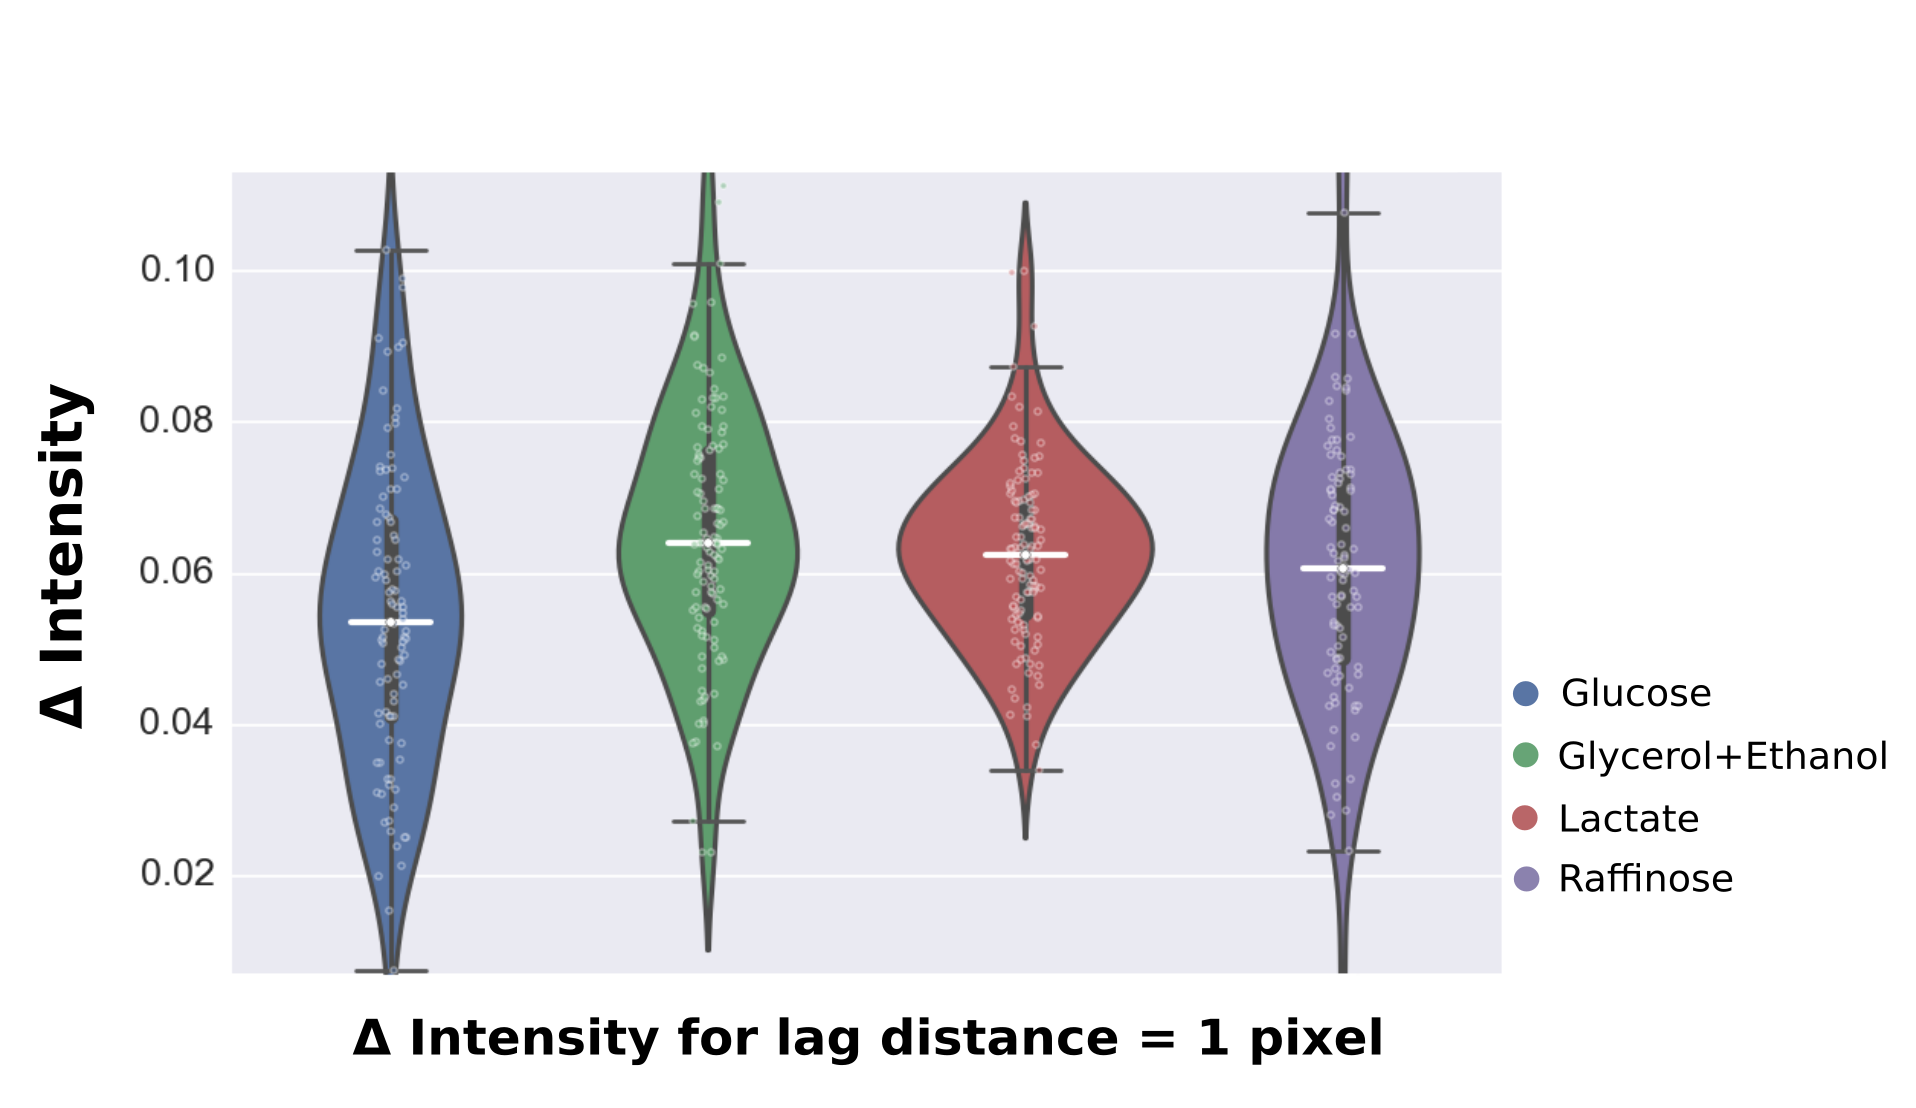
\includegraphics[width=.85\textwidth]{deltaIk1}
    \caption[Distribution for $ΔI(k=1)$]{Distribution for $ΔI(k=1)$.\\Violin plots for the distributions of $ΔI(k)$ in tubules, showing that there is a statistically significant lower value of $ΔI(k)$ at small lag distances for glucose, compared to the other three conditions which undergo respiration. Mitochondrial tubules grown in glucose have less power at high spatial frequencies.\\\emph{White bars indicate the median for the population.}}\label{fig:deltaIk1}
\end{figure}
%

We did not find a statistically significant difference in the autocorrelation curves or power spectral densities of the different growth conditions (\Fref{fig:autoactual} and \Fref{fig:psdactual}). This is evidenced by the fact that the confidence intervals indicated by the error bars overlap between the different populations.
This was surprising because we expect to see a difference between the respiratory (non glucose) and fermentative (glucose) conditions, as previously reported \cite{jimenez_mitochondrial_2014}. However it must be noted that the autocorrelation/power spectral density measures suffer from the fact that we clustered the tubules according to their lengths and it is difficult to compare all the tubules in a cell/population. The $ΔI(k)$ function (\Fref{fig:deltaIactual}) is able to obtain a more complete picture of tubule level heterogeneity across a wider range of tubule lengths. Using this method, we find a difference in heterogeneity characteristics between respiration and fermentation populations. Respiratory conditions have higher spatial frequencies and have less correlations at large length scales compared to fermentative conditions. This is evident in (\Fref{fig:deltaIk1}), where we plot the distributions of $ΔI(k=1)$. There is a statistically significant difference in the mean $ΔI(k=1)$ value between respiratory (non glucose) and fermentative (glucose) conditions (statistical test procedure done as in \fref{sec:stat}). Fermentative condition tubules have lower spatial frequencies and are more correlated over large length scales. They also seem to approach random distribution heterogeneity at a slower rate compared to respiratory tubules.
\subsection{Mitochondrial tubules in respiratory conditions have thicker width and more uniform distribution of thickness compared to fermentative conditions}
%
\begin{figure}[htp]
	\centering
    \hspace*{.5in}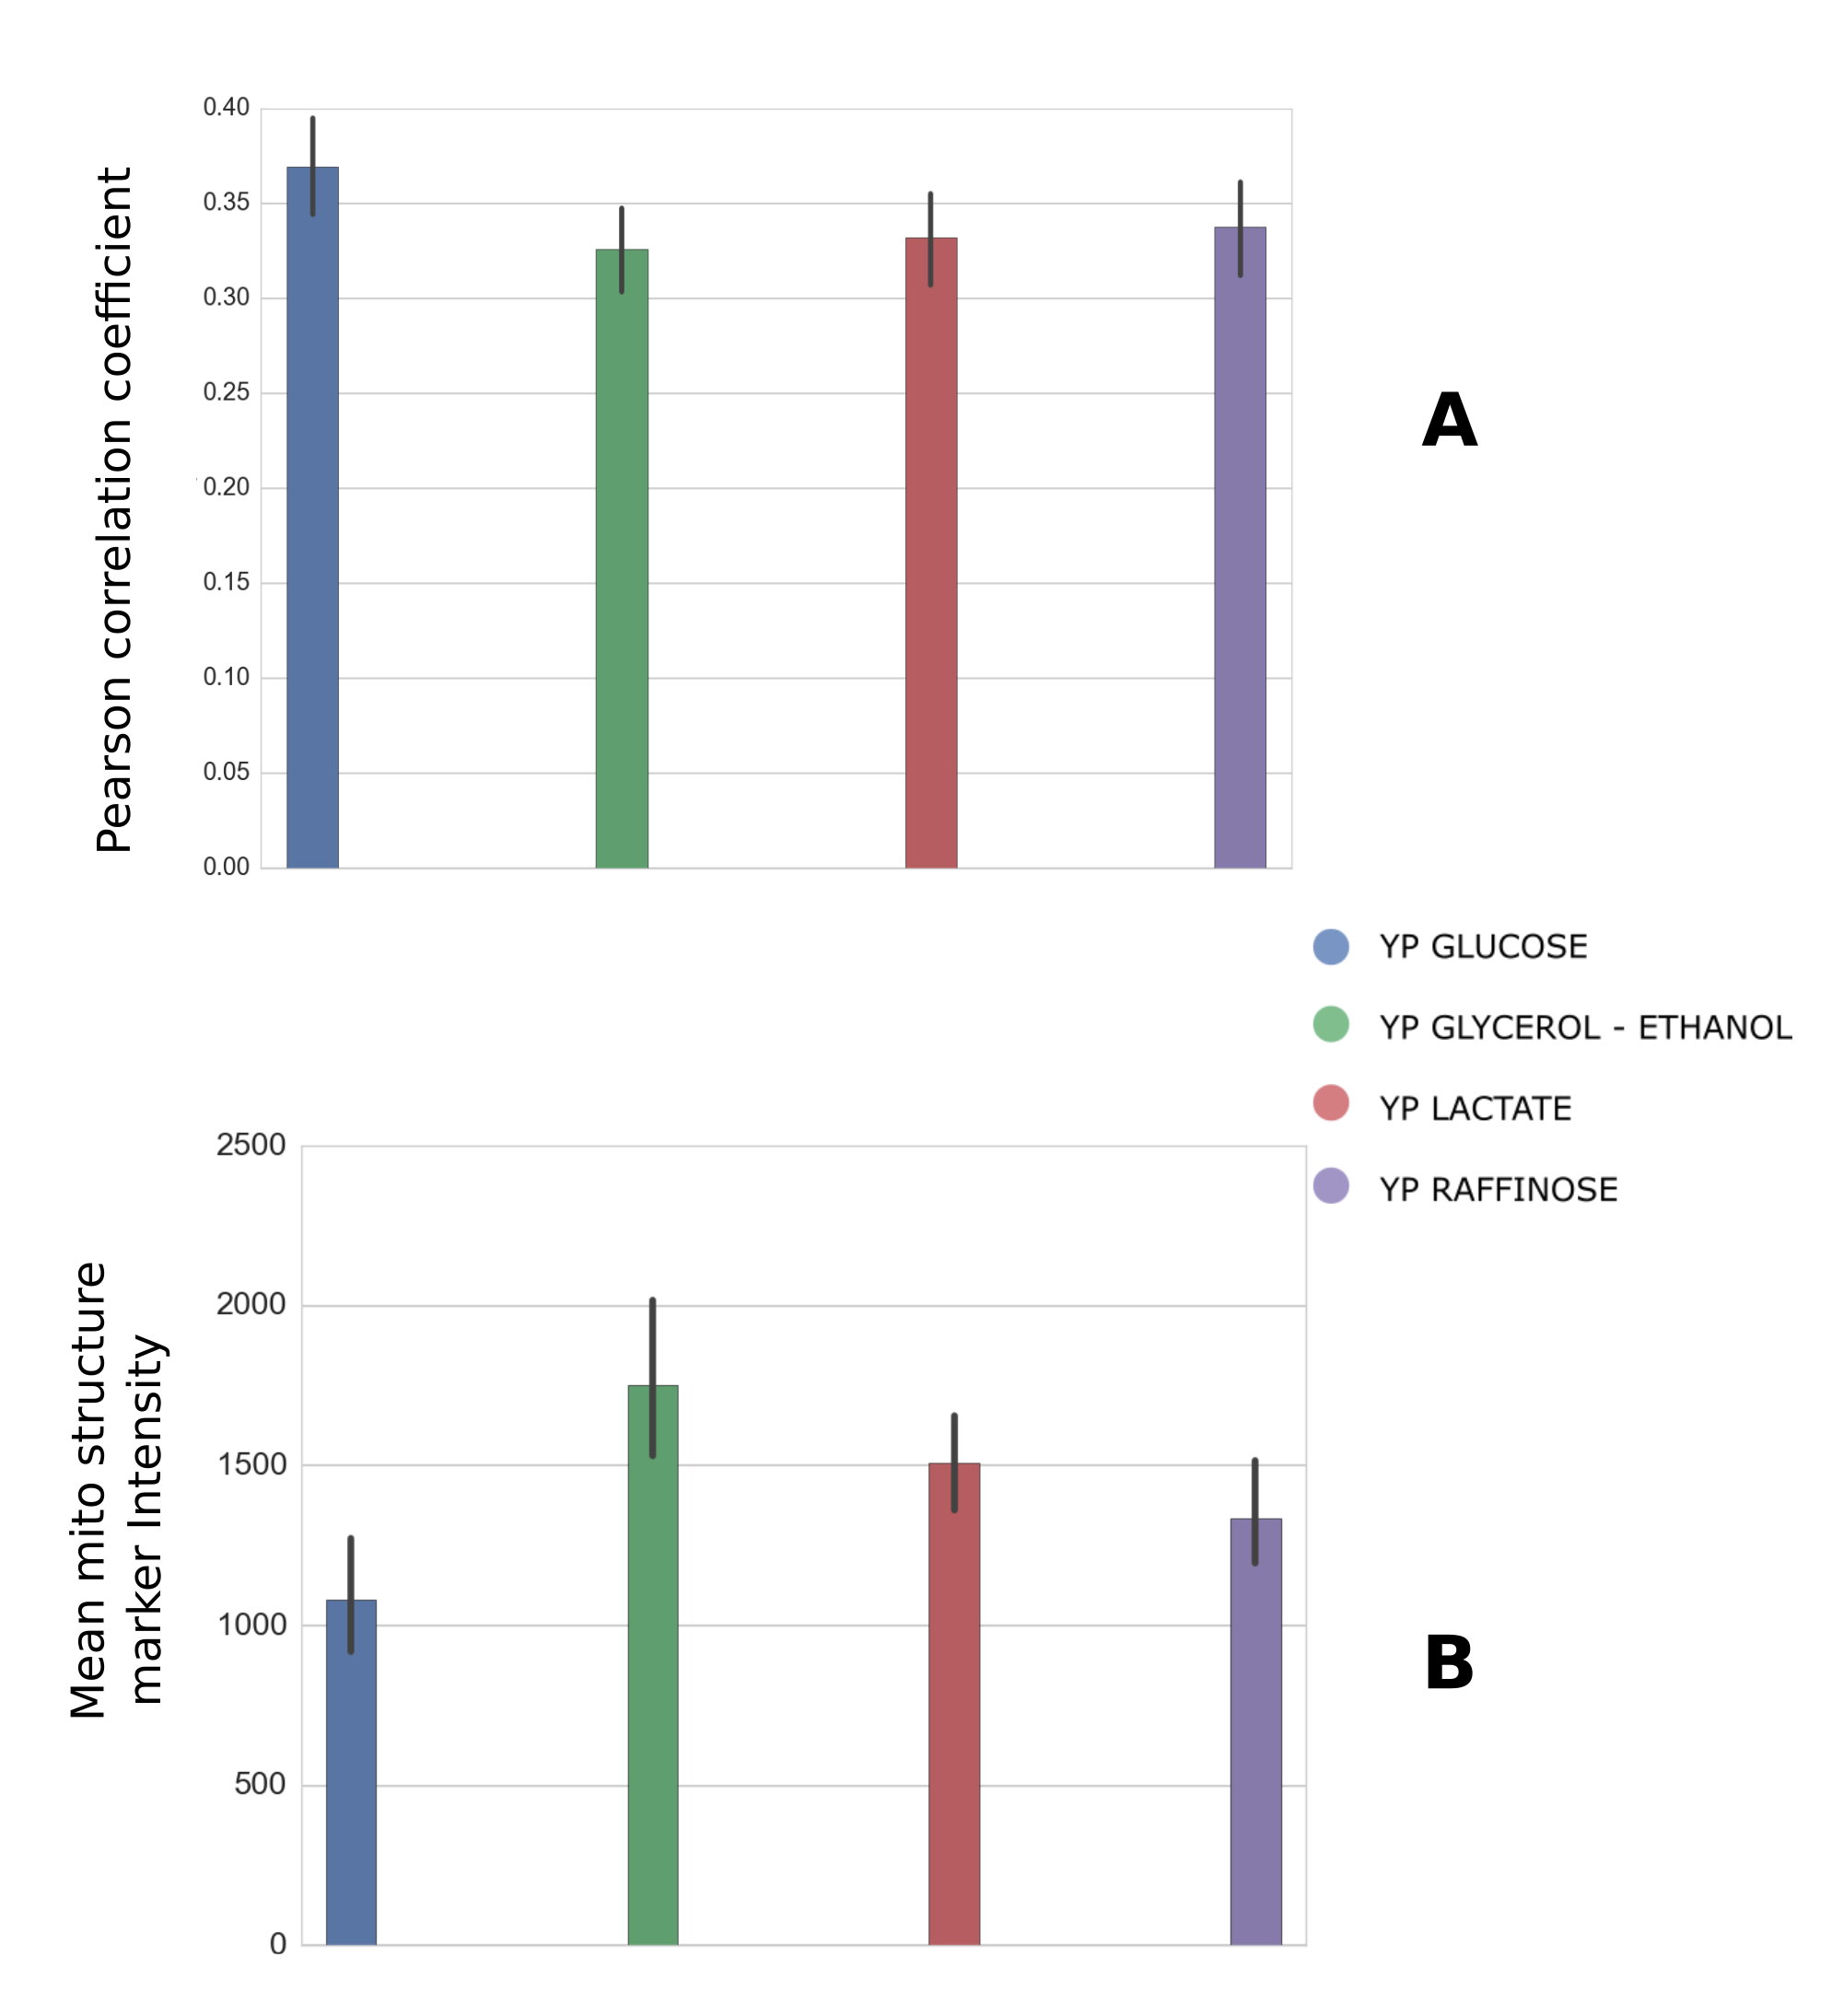
\includegraphics[width=.85\textwidth]{tubecontrol}
    \subcaptionbox{The Pearson correlation $R$ values between mitochondrial matrix marker intensity and tubule thickness show a mean value of \textasciitilde{0.35} for all the carbon conditions.\label{fig:tubecontrolA}}[\linewidth]{}
    \subcaptionbox{The variation between average (per cell) matrix marker intensity between the cells grown in different respiration conditions (non-glucose) show a large, statistically significant difference compared to the average tubule thickness shown in (\Fref{fig:tubewidth}). \label{fig:tubecontrolB}}[\linewidth]{}
    \caption[Tubule thickness variation is not an artifact of matrix intensities]{Tubule thickness variation is not an artifact of matrix intensities.\\Mitochondrial matrix marker intensities do not show strong correlation with tubule thickness (\Fref{fig:tubecontrolA}). The variation in matrix intensity is also much higher than the variation in tubule thickness (\Fref{fig:tubecontrolB}). Therefore measurements of tubule thickness derived from MitoGraph v2.0 are likely not affected by variations in matrix marker intensities.\\\emph{Error bars represent the bootstrapped 95\% confidence interval of the mean.}
}\label{fig:tubecontrol}
\end{figure}
%
%
\begin{figure}[htp]
	\centering
    \hspace*{.75in}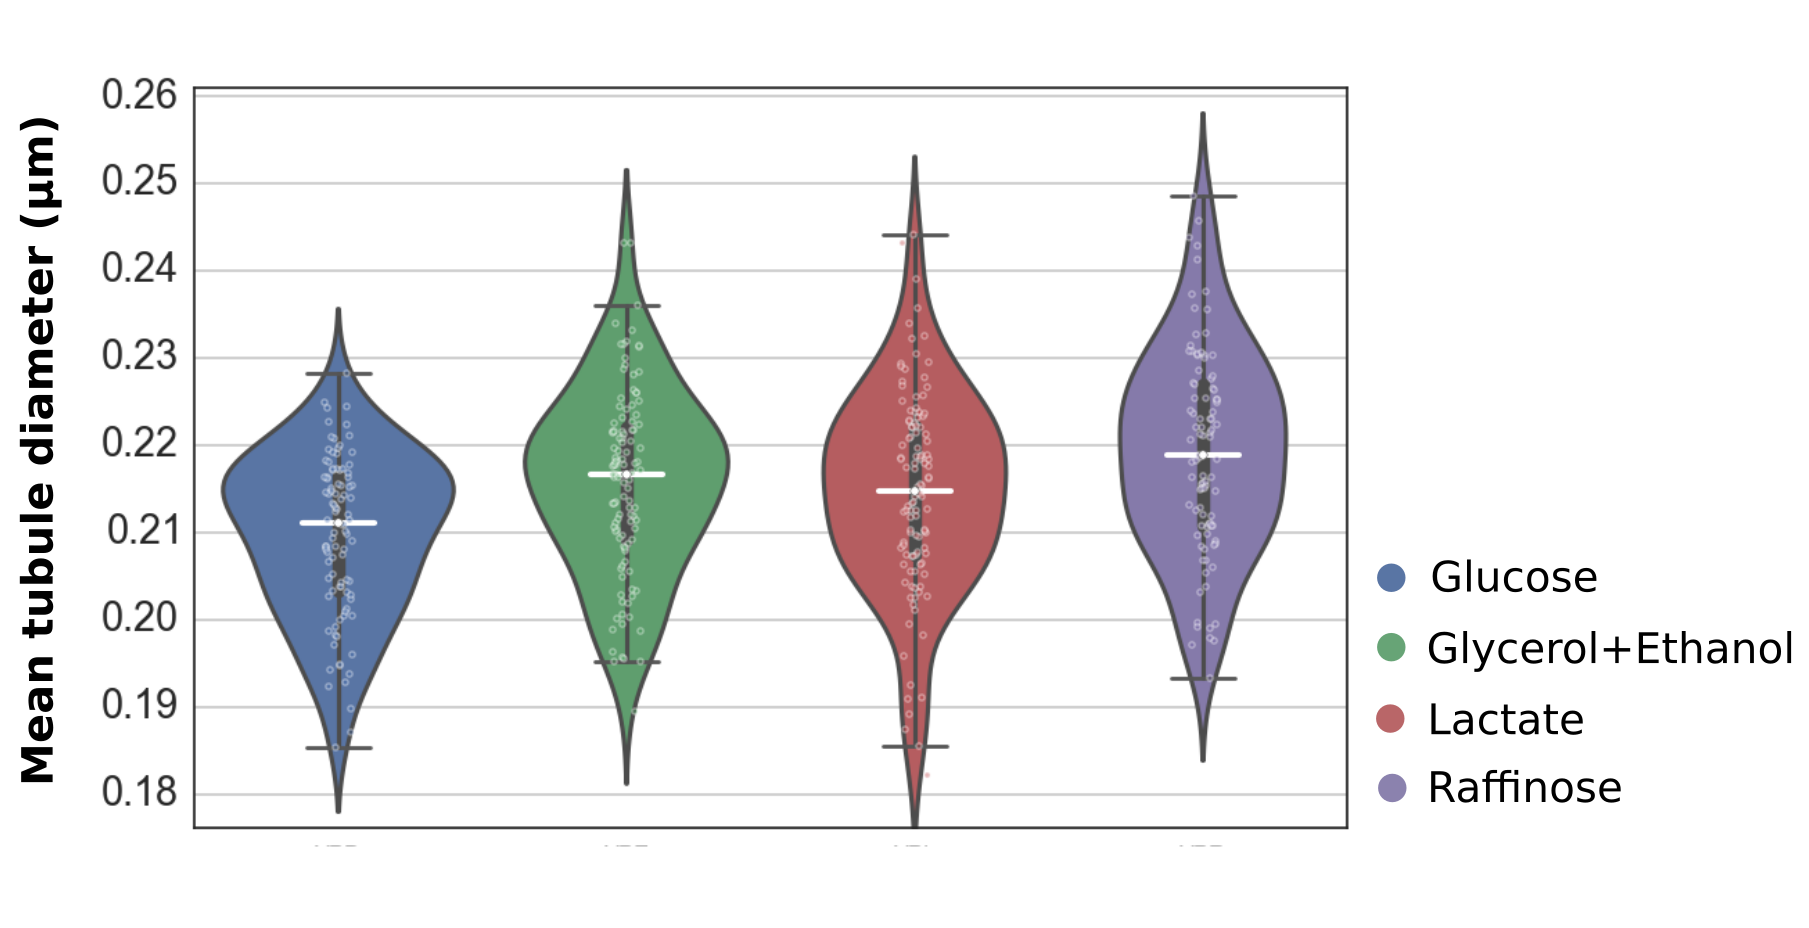
\includegraphics[width=.85\textwidth]{tubewidth}
    \caption[Distribution of mean tubule diameter per cell per population]{Distribution of mean tubule diameter per cell per population.\\The mean tubule diameters in respiration (non glucose) are statistically greater than the tubules in fermentation. The tubules are on average 2.6\% greater than in glucose.\\\emph{White bars indicate the median value.}}\label{fig:tubewidth}
\end{figure}
%
%
\begin{figure}[htp]
	\centering
    \hspace*{.5in}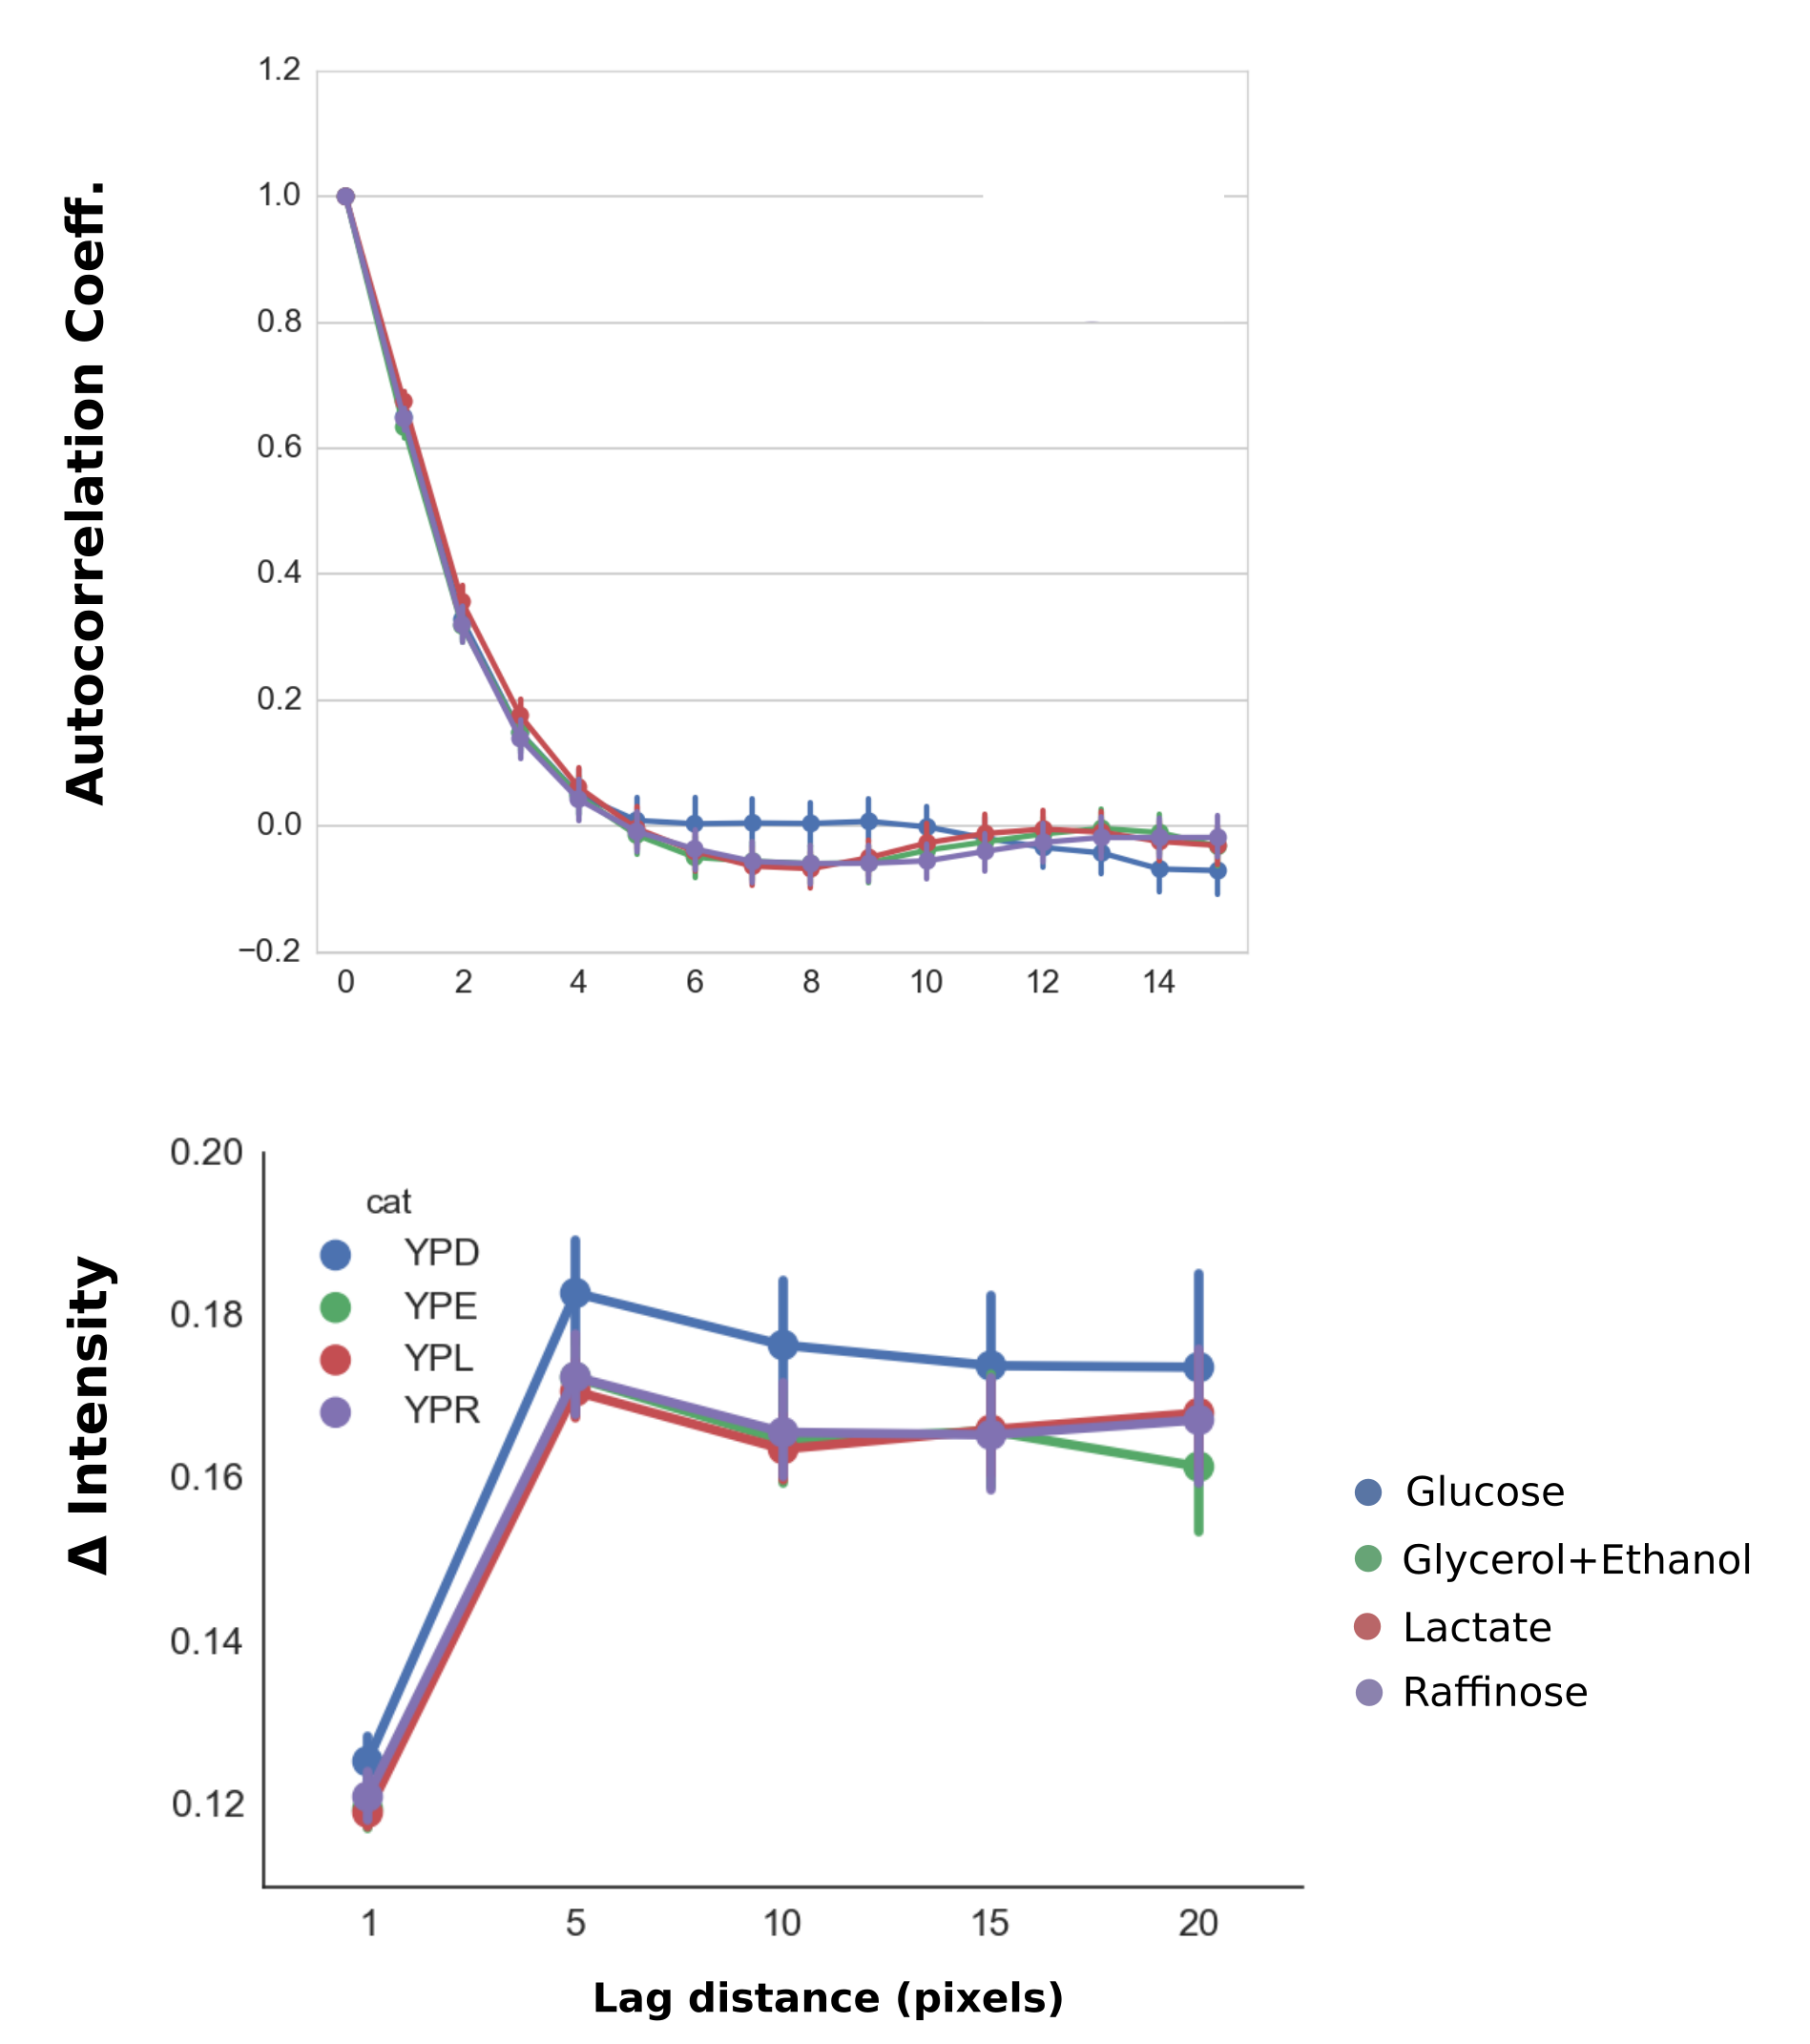
\includegraphics[width=.85\textwidth]{tubewidedist}
    \caption[Autocorrelation and $ΔI(k)$ curves of tubule diameter heterogeneity]{Autocorrelation and $ΔI(k)$ curves of tubule diameter heterogeneity.\\The $ΔI(k)$ curve for tubule diameter indicate that tubules grown in glucose (fermentation) have a higher tubule thickness heterogeneity at small length scales/lag distances. No statistical difference were seen in the autocorrelation curves for tubule diameter.\\\emph{Error bars represent the bootstrapped 95\% confidence interval of the mean.}}\label{fig:tubewidedist}
\end{figure}
%

It has been reported that mitochondrial tubules growing in glycerol as the sole carbon source had a 6\% thicker tubule diameter compared to cells growing in glucose \cite{egner_fast_2002}. We analyzed the tubule diameter of our data using an algorithm in MitoGraph v2.0 that calculates the radius of the tubule at any point along the skeleton based on the surface rendered image of the tubule. Standard image intensity segmentation of tubules tend to result in brighter tubules having a wider segmentation diameter (in other words appear thicker). MitoGraph v2.0 uses various image processing techniques to segment the mitochondrial tubule from the background image in a way that is independent of the image intensity of the tubules. In order to validate this, in (\Fref{fig:tubecontrolA}) we show the correlation between the mean intensity for the mitochondrial structural marker (mRuby2, a matrix targeted fluorescent protein, \fref{sec:strain}) and the mean tubule width is low (\textasciitilde{0.35}) and importantly, not significantly different across the four carbon sources. This means that any difference seen in tubule width between the conditions is not due to intensity variations between the conditions. In addition, in (\Fref{fig:tubecontrolB}), the variation in mitochondrial structural marker intensity between the three respiratory conditions is significantly different, while the variation of the tubule width among the three conditions is not. In other words, the variation in image intensity is much higher than the variation in tubule thickness, thus we feel confident in reporting our tubule thickness results are not due to an artifact of image segmentation.

In \Fref{fig:tubewidth} we see that there is a statistically significant difference in tubule diameter between populations in respiration and fermentation. Mitochondrial tubules undergoing respiration have an average 2.6\% thicker tubule diameter compared to tubules undergoing fermentation. There was no difference in tubule diameter between the three respiratory conditions. Statistical testing was done as in \fref{sec:stat}.
When comparing the heterogeneity of the tubule thickness distributions (\Fref{fig:tubewidedist}), we do not see a difference in the autocorrelation curves between tubules in respiration and fermentation. However when comparing the $ΔI(k)$ curves, there is a statistically significant higher value of $ΔI(k)$ at lag distances of 1 pixel for the fermentative condition compared to the respiratory condition. Therefore we conclude that tubules in fermentation have a higher tubule thickness heterogeneity compared to in respiration. 
\section{Discussion}
In the study by Jimenez et al. \cite{jimenez_mitochondrial_2014}, they showed that ATP synthase cluster into discrete domains, which they called F1F0-cluster domains. Importantly, they showed that these domains were localized to cristae membrane regions. They also showed that as growth condition was altered from a fermentative to respiratory state, the number of these cluster domains increased. Our results in \fref{sec:432} and \Fref{fig:deltaIactual} showed that mitochondrial tubules in fermentation have ΔΨ distributions with lower spatial frequencies and are correlated at larger length scales. In the Jimenez study they showed that the F1F0 cluster domains were widely separated in glucose grown cells. They also showed that as the number of these cluster domains increased, the signal from the fluorescent protein markers for these cluster domains would 'smear' out as the distance between the cluster domains would be so small as to be unresolvable optically in their confocal microscope system. If we consider that F1F0-cluster domains are regions with high OXPHOS activity we can reasonably predict that these domains would be regions with high ΔΨ. If the regions with high ΔΨ are separated by large distances, they will show a correlation at large length scales. This explains our results for tubules in respiration (\Fref{fig:deltaIactual}). Conversely in respiratory conditions where the F1F0-cluster domains are spaced closed to each other, ΔΨ intensity will show correlation at small length scales (their spectral density will have a high power component at high spatial frequencies). An important contribution of our study in this chapter is that we showed that this heterogeneity in ΔΨ was not just an artifact of random ΔΨ intensity variations. Furthermore we observed heterogeneity of ΔΨ even in respiratory conditions, which the Jimenez study could not as their method could not distinguish the signal variations when the F1F0- cluster domains were very close.

Similar to a study by Egner et al. \cite{egner_fast_2002}, we observed that mitochondrial tubule diameter increased when grown under respiratory conditions. The magnitude of the increase is about half that reported (\textasciitilde{3\%} vs 6\%), likely due to differences in optical resolution between our systems. The Egner study used 4Pi microscopy with optical resolution below the diffraction limit, and thus it is not surprising they observed larger tubule width differences. In fact analysis of electron microscopy (EM) based cross sections of mitochondrial tubules showed that tubules in glucose had a mean diameter of about \SI{350}{\nm} \cite{baba_three-dimensional_1989,watson_organization_1972} and about \SI{400}{\nm} in lactate \cite{vogel_dynamic_2006,yotsuyanagi_[study_1962}. While different imaging methods show different magnitudes of tubule width increase when moving between fermentation and respiration, it is clear that mitochondria tubules become thicker when they undergo respiration. This is likely due to the increased number of cristae that is apparent in the EM images of mitochondrial tubules undergoing respiration. What is novel in our results however, is that we report a change in the distribution of the thickness variation along a tubule between respiration and fermentation. Specifically tubules from cells grown in glucose exhibited higher thickness variations at small length scales compared to respiratory conditions. The fluorescent marker used to label mitochondria marker was targeted to the matrix. Our results seem to indicate that the mitochondrial matrix marker distribution in glucose grown cells experience some sort of constriction at length scales smaller than in respiratory condition cells. This is interesting because according to a previous study \cite{mannella_structure_2006} mitochondria in low respiration states (State 4) have less number of cristae, and presumably a less constricted matrix lumen (\Fref{fig:matrix}). One possible way to resolve this mystery is to label the outer membrane instead, to see if this tubule thickness heterogeneity result holds.
%
\begin{figure}[htp]
	\centering
    \hspace*{.65in}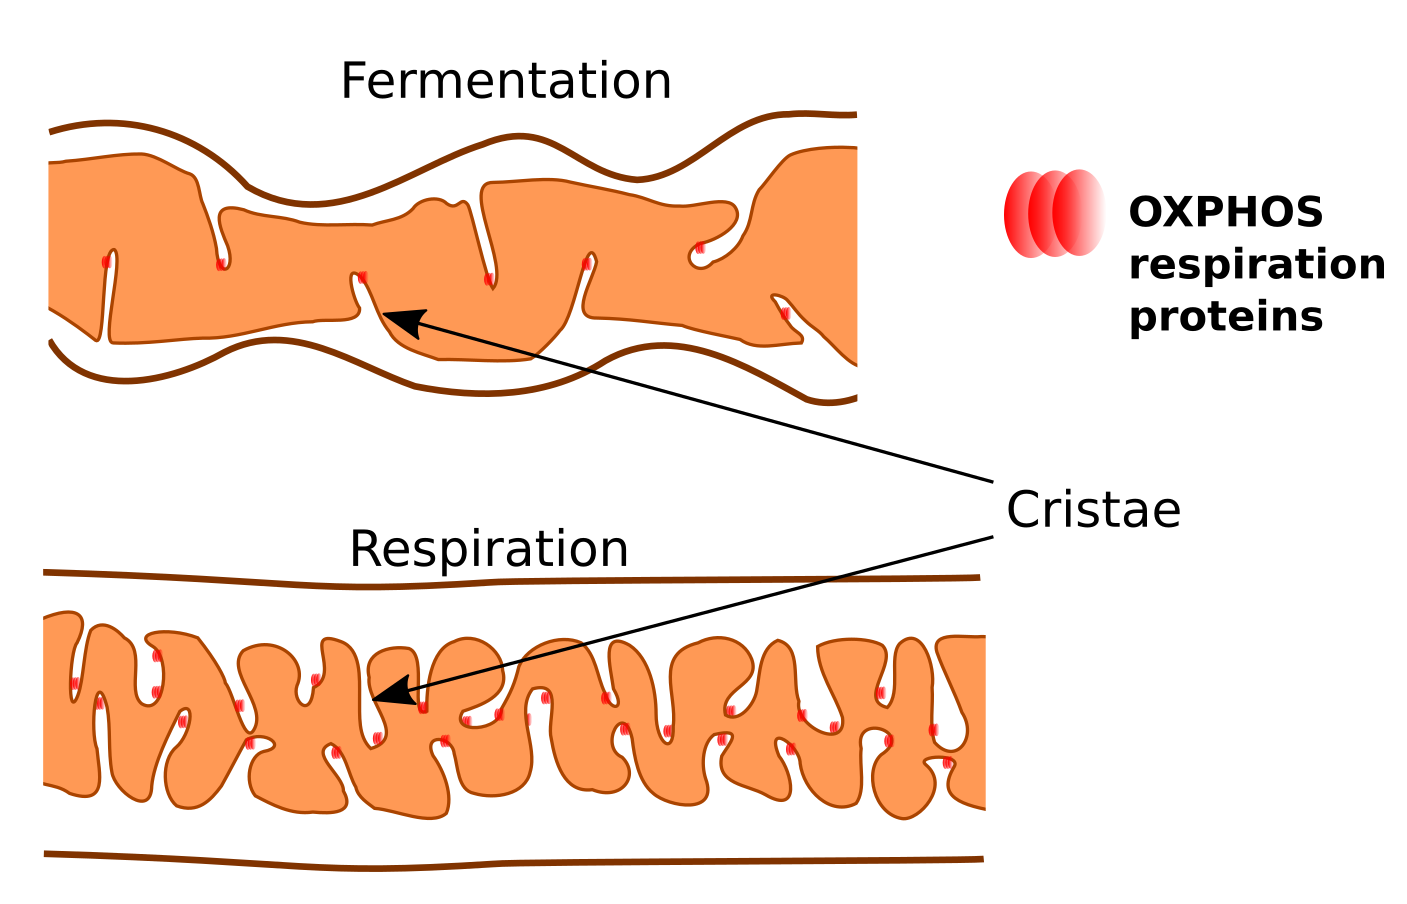
\includegraphics[width=.85\textwidth]{matrix}
    \caption[Mitochondria ultrastructure changes due to respiratory state]{Mitochondria in respiratory conditions display less heterogeneity in cristae density and tubule thickness compared to fermentative conditions.}\label{fig:matrix}
\end{figure}
%

It is interesting to note in our result that we see no significant differences in the heterogeneity characteristics of mitochondria tubules (both ΔΨ and tubule width) grown in the different respiratory conditions (i.e. glycerol+ethanol, lactate and raffinose). One possibility is that respiration states are similar in the three carbon sources, hence no changes in the IMM would be expected. Another possibility is that changes in the IMM are so subtle among the respiratory conditions that they are not resolvable by the optics of the system.

Between the two, we favor the second explanation because from our results in \Fref{ch:three}, we know that the respiration rates are different among the three respiratory carbon sources. One way to test this is to try to inhibit a respiration pathway that is specific to just a subset of the carbon sources. For example it is known that lactate oxidation happens directly at the \emph{lactate:cytochrome c} oxidoreductase complex. Yeast cells are able to grow normally on lactate substrate when given Antimycin A, a respiratory chain inhibitor that blocks the transfer of electrons to cytochrome b, which is positioned upstream of the \emph{lactate:cytochrome c} oxidoreductase complex. Thus it would be expected that under Antimycin A, yeast grown in raffinose would exhibit heterogeneity characteristics more similar to that of glucose (fermentation) while lactate would still retain normal respiratory heterogeneity characteristics. Yeast cells would not be able to grow in glycerol+ethanol when given Antimycin A as it has to undergo respiration.

Another interesting followup would be to use a fluorescent protein marker tagged to the ATP-synthase subunit (similar to the Jimenez study) and apply a membrane potential dye to see if the F1F0-cluster domains really co-localize with local membrane potential heterogeneity. One difficulty would be that we would not be able to use our mitochondrial matrix targeted marker with mRuby2 as the ATP-synthase would need to use the emission and excitation spectrum that mRuby2 lies in. This could be overcome by tagging either the ATP-synthase or the matrix targeted marker with a blue excitation/emission fluorescent protein.






\chapter{Membrane potential heterogeneity at the mitochondrial network level}\label{ch:five}
\clearpage
\section{Introduction}
Mitochondria in yeast form a tubular network along the inner periphery of the cell. The mitochondrial network undergoes dynamic remodeling by fission and fusion events. The function and mechanisms of these remodeling events have been an active research field for the last two decades \cite{hoitzing_what_2015}. The proteins that play an essential role in mitochondrial fission and fusion dynamics belong to the Dynamin family. In yeast, the key proteins are MGM1, FZO1 and DNM1. MGM1 (OPA1 in mammalian cells) mediates inner mitochondrial membrane fusion, FZO1 (mitofusin MFN1 and MFN2 in mammalian cells) mediates outer mitochondrial membrane fusion while DNM1 (DRP1 in mammalian cells) mediates fission. Fission and fusion rates are balanced \cite{shaw_mitochondrial_2002}. Deletion or knockdown of fusion related proteins result in a highly fragmented network while deletion of fission proteins result in a highly branched, 'net-like' structure \cite{shaw_mitochondrial_2002}. Inhibition of fusion and fission results in a host of cellular defects resulting from OXPHOS deficiencies, mtDNA loss and increased ROS production \cite{chen_disruption_2005,ishihara_regulation_2006,nunnari_mitochondria:_2012}. In humans, mutations in the fusion related proteins MFN2 and OPA1 result in mitochondrial and neurodegenerative diseases such as Charcot Marie Tooth, dominant optic atrophy (DOA), Parkinson's and Alzheimer's disease \cite{alexander_opa1_2000,bliek_mechanisms_2013,wang_impaired_2009}.

The severe consequences of the loss of mitochondrial fusion related proteins imply that mitochondrial fission and fusion dynamics is tightly integrated with cellular bioenergetics \cite{sauvanet_energetic_2010}. Fusion promotes a connected network which is hypothesized to mediate faster and more effective mixing of mitochondrial proteins \cite{busch_quality_2014,wilkens_restricted_2013}. A fused mitochondrial network has also been hypothesized to mediate an increase in ATP production via several pathways including changes to the cristae curvature \cite{patten_opa1-dependent_2014}, decrease in proton leak \cite{gnaiger_mitochondrial_2002} and by serving as a transmission power cable \cite{amchenkova_coupling_1988}. This transmission power cable hypothesis says that fused mitochondrial networks enable the electrochemical gradient from one end of the network to be used at another end. Mitochondrial dynamics are required for mitochondrial quality control \cite{twig_fission_2008}. In this process, a healthy mitochondrial network is maintained by segregation/fission of mitochondrial fragments from the network and selective fusion of those fragments back to the network. Selective fusion means that only fragments above a certain quality threshold (as measured by mitochondrial membrane potential, ΔΨ) can fuse back to the network \cite{legros_mitochondrial_2002,meeusen_mitochondrial_2004}. Because healthy mitochondria are more likely to fuse to the network, most of the observed isolated fragments of mitochondria will be those that are unhealthy/below the threshold for ΔΨ. Fission can be thought of as a way for the network to protect itself from unhealthy mitochondrial fragments. According to the mitochondrial quality control model, isolated mitochondrial fragments that are unable to fuse back to the network are targeted for degradation by the autophagic machinery, a process know as mitophagy.
%
\begin{figure}[htp]
	\centering
    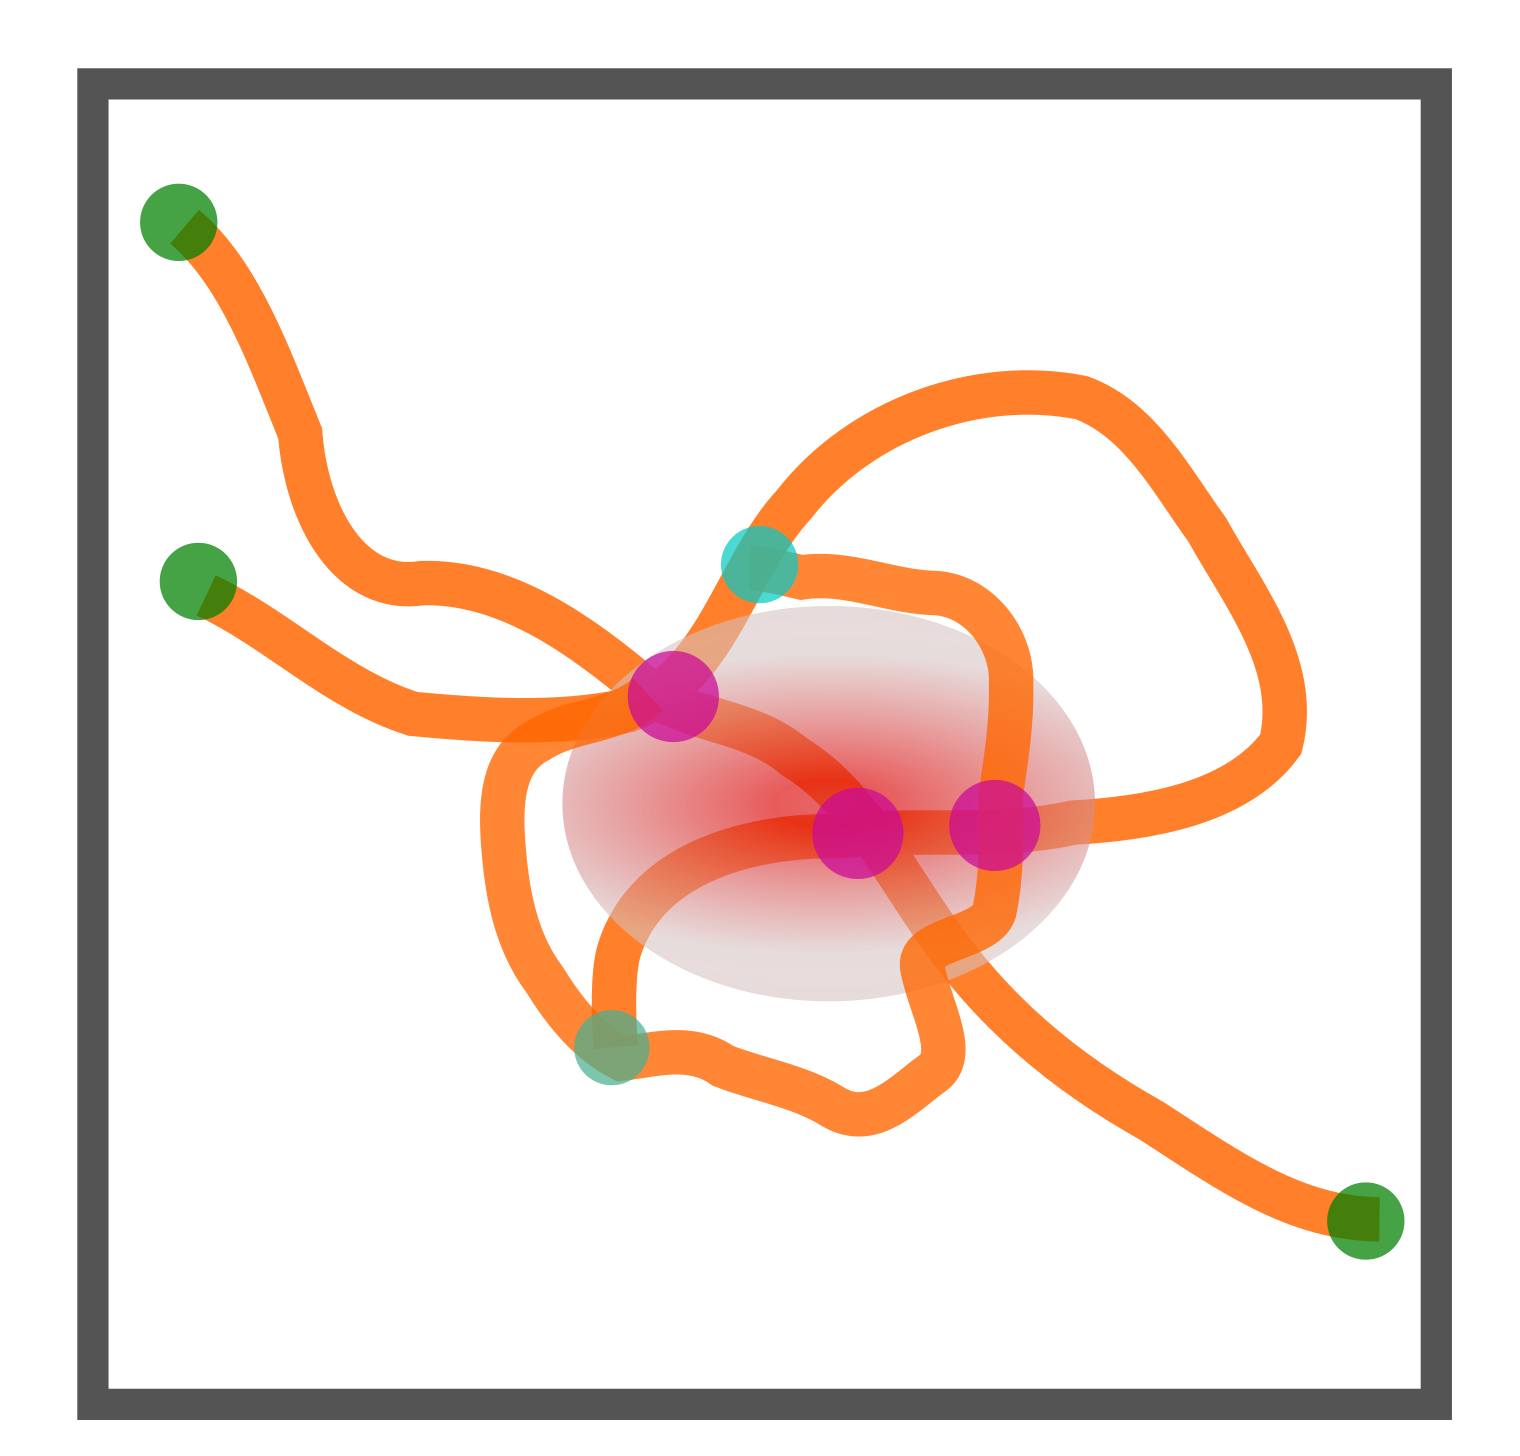
\includegraphics[width=.5\textwidth]{cartoon}
    \caption[Heterogeneity of structure-function in mitochondrial networks]{Heterogeneity of structure-function in mitochondrial networks.\\Shown here is a region of a mitochondrial network within a yeast cell. Branchpoints representing the intersection of mitochondrial tubules are shown as the cyan and magenta nodes. The area in red is a region of high connectivity because the magenta nodes have a higher degree of connectivity (they are connected to more connected nodes) compared to the cyan and green nodes. Our hypothesis is that these sites are enriched for ΔΨ based on the increased rate of fusion events occurring in these regions.}\label{fig:cartoon}
\end{figure}
%

Mitochondrial quality control via fission and fusion dynamics imply some level of heterogeneity in the distribution of ΔΨ within the network. Functional complementation through fusion based mixing and segregation of unhealthy mitochondria through fission would be unnecessary if mitochondrial quality (as indicated by ΔΨ) was homogeneous throughout the network. Previous studies have relied on qualitative descriptions of changes in mitochondrial morphology when undergoing a change in respiration states \cite{jakobs_spatial_2003,sesaki_division_1999}. They did not directly quantify the relationship between the topology of the mitochondrial network and its functional state. In this chapter we investigate the relationship between mitochondrial network structure (topology/connectivity) and functional heterogeneity (ΔΨ) in mitochondrial networks, i.e. whether structural features of regions within the network is indicative of the bioenergetic state of that region (\Fref{fig:cartoon}). 

The first area that we investigate is the relationship between mitochondrial network connectivity and the density of mitochondrial tubules at the cell surface. We define surface density as a measure that represents how 'packed' with mitochondrial tubules a given cell surface is. We expect that network connectivity should scale with surface density of the network, because mitochondrial tubules in denser networks would have a higher probability of encountering and fusing with another tubule. In addition we expect to see a clear difference between mitochondrial networks in fermentation and respiratory conditions. When yeast cells are grown in a non-fermentable substrate, the mitochondrial volume as a proportion of cell volume (volume ratio) increases dramatically \cite{jakobs_spatial_2003}. Mitochondria in glucose (fermentation) form very simple networks, with few branching points, while mitochondria in glycerol (respiration inducing) form networks that are more branched and elaborate \cite{egner_fast_2002}. We investigate the connectivity at the global (whole cell) and local (part of the cell) level in response to changes in surface density brought about by cells growing in different carbon sources (details in \fref{sec:carbon}).  We also expect to see a difference in the connectivity measures of mitochondrial networks grown in the three different respiration inducing carbon sources (lactate, glycerol+ethanol and raffinose) based on their overall oxygen consumption rate (OCR) and ΔΨ levels (\Fref{fig:O2dy}). 

The second area we investigate is the relationship between surface density, network connectivity and mitochondrial membrane potential (ΔΨ). We hypothesize that surface density should scale with ΔΨ. Since respiratory conditions induce a change in volume ratio and surface density of mitochondria in a cell, and respiration requires ΔΨ, we expect that there will be some sort of relationship between the surface density of mitochondria and the overall level of ΔΨ. Furthermore, it has been suggested by observation that conditions that result in highly connected networks tend to favor more fission and fusion events \cite{jakobs_spatial_2003}. Therefore we hypothesize that ΔΨ scales with mitochondrial network connectivity. This is due to the selective fusion mechanism where only mitochondria that are functional/healthy can fuse back to the network. 

We also investigate specific regions of the mitochondrial network known as branching points. These are the intersections of tubules within the network (\Fref{fig:cartoon}, red and cyan dots). Branching points are by definition sites of higher connectivity compared to non branching point regions. Therefore on average, more fusion events might take place in these regions, and therefore by the selective fusion principle they might display a higher ΔΨ level. Therefore we hypothesize that branching points within a network might have a higher level of ΔΨ compared to the rest of the network.

Lastly, we investigate the ΔΨ levels of isolated fragments of mitochondria. Based on the mitochondrial quality control model that says that isolated fragments of mitochondria that are unable to fuse back to the network are targeted for mitophagy, we expect these fragments to have a lower level of ΔΨ compared to the network. Furthermore because mitophagy selection is size dependent (i.e. only fragments below a certain size can undergo mitophagy) \cite{kanki_mitophagy_2008,rambold_tubular_2011} we expect smaller isolated fragments to have a lower ΔΨ compared to longer isolated fragments.
%
\begin{figure}[htp]
	\centering
    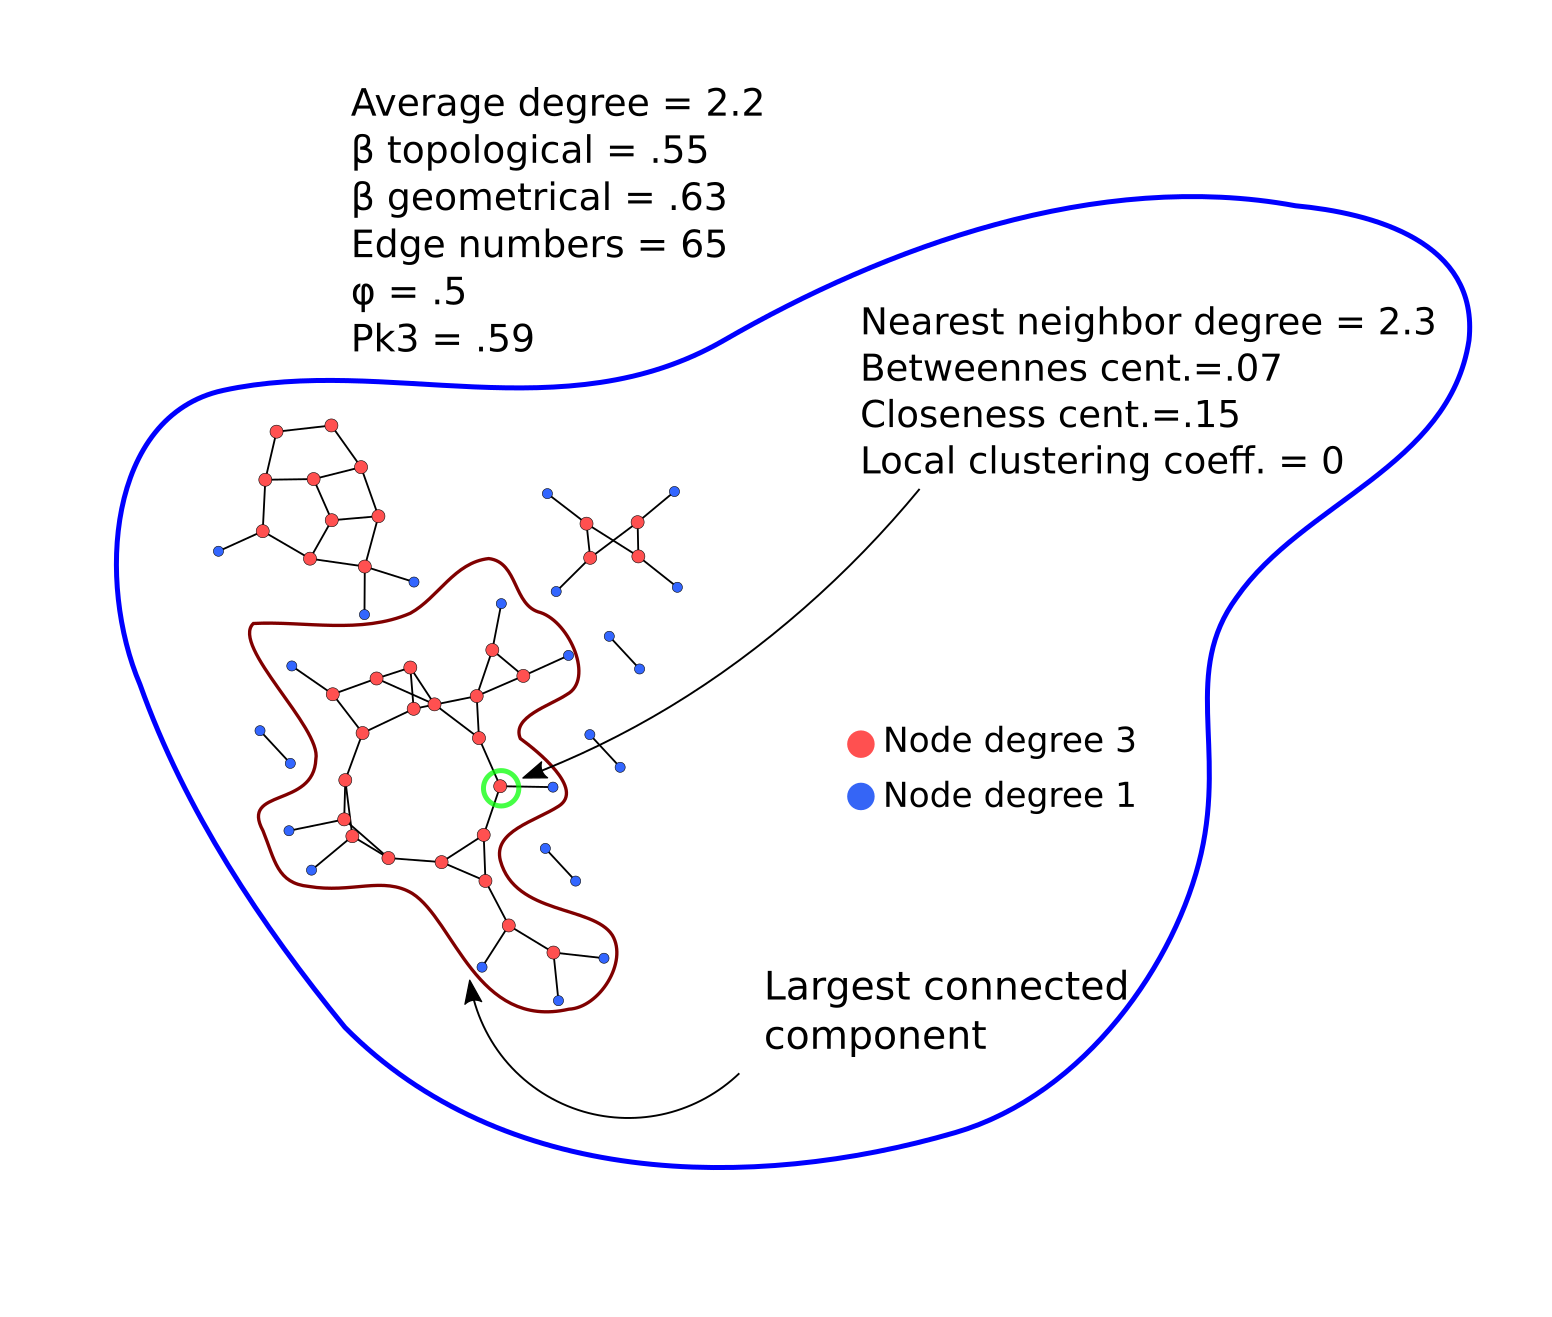
\includegraphics[width=.95\textwidth]{graph}
    \caption[Global and local connectivity in mitochondrial networks]{Global and local connectivity in mitochondrial networks.\\Shown here is a graph representation of a real mitochondrial network. Branching points representing the intersection of edges/tubules in the network are shown as red nodes, while the ends of the tubules are shown as blue nodes. The largest connected component circled in red is the largest completely connected entity in the graph. The measures outside the blue outline represent the global connectivity measures of the entire network/graph (area circled in blue). Global connectivity gives an overall measure of how interconnected the network is. The measures inside the blue outline represent the local connectivity measures of the network. Local connectivity measures shows the connectivity related to a region of the graph, hence they are tied to a particular node in the graph, for e.g. the local connectivity numbers shown are for the node circled in green.}\label{fig:graph}
\end{figure}
%
\section{Materials and Methods}
\subsection{Data structure}
The data calculated in this chapter utilizes the database structure as detailed in \fref{sec:database}. It consists of structural (area, length, volume), topological (network connectivity measures) and functional parameters (respiration, ΔΨ levels) organized at a per tubule, per cell and per population (carbon source) level. This allows analysis to be carried out at the scale appropriate to each question. For most of this chapter data is considered at the per cell level. However when we investigate branchpoint heterogeneity we query at the per tubule level since we interrogate the regions around a branchpoint, which consists of intersecting tubules. 

In this chapter we consider each mitochondrial network of a cell to be a planar, undirected graph. A planar graph is a graph that can be embedded in a plane, which means it can be drawn within a plane such that no edges cross each other \cite{west2001introduction}. A graph (\Fref{fig:graph}) has edges (corresponding to the tubules of a mitochondrial network) and nodes (corresponding to the ends of the individual tubules). The graphs were derived from the VTK spatial information output of MitoGraph v2.0 using the NetworkX (\url{https://networkx.github.io/}) module in Python. If a measure was specified as topological, each edge was considered to have a length of one (i.e. an unweighted graph). If a measure was specified as geometric, the edges of the graph had a weight equal to the real spatial length (in microns) of the tubule it represented.
 
\subsection{Surface density as a measure of spatial density of mitochondria}
Spatial density of mitochondria is a measure of how densely a mitochondrial network fills a given space. It can be expressed as volume ratio \cite{rafelski_mitochondrial_2012}, which is the proportion of the volume of the cell that consists of the mitochondrial network or it can be given as the surface density.
Volume ratio is appropriate when one is concerned only with the amount of mitochondria in a cell, for example when normalizing OCR to mitochondrial content. However in the context of this chapter where we are concerned with how the spatial density of mitochondria on the cell surface affects the connectivity of the network, surface density if more appropriate.  

The surface area $S$ of a cell which we assume is in the shape of a prolate ellipsoid ($a=b, c >a$, where $a$ is the minor axis and $c$ the major axis of the ellipsoid) is given by the formula \cite{olver_nist_2010}:
\begin{equation}
	\begin{split}
		\begin{aligned}
			S&=2\pi a^2 \left( 1+\frac{c}{ae} \arcsin(e)\right) \\[2ex]
			e&=\sqrt{1-\frac{a^2}{c^2}}
		\end{aligned}
	\end{split}
\end{equation}
We define the surface density of the mitochondrial network as:
\begin{equation}\label{eq:surfd}
	\begin{split}
		\begin{aligned}
			q&=\frac{L}{S}\\
			L&=\text{total length of mitochondrial network} \\
			S&=\text{surface area of cell}
		\end{aligned}
	\end{split}
\end{equation}
\subsection{Global and local measures of connectivity}
We use standard network theory terminology when defining measures of connectivity in the mitochondrial network, which we consider to be an undirected planar graph \cite{west2001introduction}. In this type of graph, the largest connected component is the largest subgraph with no unconnected /isolated edges (circled red in \Fref{fig:graph}). The degree of a node is defined as the number of edges connected to that node. For example, nodes at the ends of a graph have a degree of one. A branchpoint in our graph is a node with a degree of at least three. The average degree of all nodes in the network is often used as a standard measure of network connectivity.

\emph{Global Connectivity} measures are connectivity measures that relate to the whole network. These measures include:
\begin{equation}
	\begin{split}
		\begin{aligned}
			& \text{φ}=\text{Fraction of nodes in the largest connected component} \\
			&\text{β}_{\V{geometric}} = \text{Fraction of edges in largest connected component}\\
			&\text{β}_{\V{topological}} = \text{Fraction of total length of the largest connected component}\\
			& \mathrm{Pk_3} =\text{Fraction of nodes that have three edges}\\
			&\text{Network average degree} = 2\times \frac{\text{number edges}}{\text{number of nodes}}\\
			& \text{Number of edges in the graph}
		\end{aligned}
	\end{split}
\end{equation}
\emph{Local Connectivity} are measures that reflect the connectivity of specific regions within the network. These measures consist of:

\emph{Nearest neighbor degree} of a node is the average degree of all directly adjacent nodes. \\
\emph{Betweenness centrality} of node $v$ is given by \cite{brandes_faster_2001}:
\begin{equation}
	\begin{split}
		\begin{aligned}
			&B(v)=\displaystyle\sum_{s,t \in V} \frac{\sigma(s,t|v)}{\sigma(s,t)}\\
			&\text{where $\sigma(s,t)$ is the number of shortest paths}\\[-1.5ex]
			&\text{between nodes $s$ and $t$}\\
			&\sigma(s,t|v)\text{ is the number of shortest paths between $s-t$ }\\[-1.5ex]
			&\text{passing thru $v$ not including $s-t$}\\
			&\text{$V$ is the set of all nodes}
		\end{aligned}
	\end{split}
\end{equation}
The betweenness centrality is a measure of how 'essential' a node is to the connectivity of a network; a high value means a node forms a vital link between the connections of many pairs of nodes.\\
\emph{Closeness centrality} of a node v is given by \cite{freeman1979centrality}:
\begin{equation}
	\begin{split}
		\begin{aligned}
			&C(v)=\frac{n-1}{\displaystyle\sum_{v=1}^{n-1} d(v,u)} \\
			&\text{where $n$ is the number of nodes}\\
			&\text{$d(v,u)$ is the shortest path distance between $v$ and $u$}
		\end{aligned}
	\end{split}
\end{equation}
A high closeness centrality indicates that the node v has small distances to all other nodes. The numerator is a normalization factor to account for the fact that the sum of distances scales with the number of nodes.\\
\emph{Clustering coefficient} of a node v is given by \cite{saramaki2007generalizations}:
\begin{equation}
	\begin{split}
		\begin{aligned}
			&K(v)=\frac{2 T(v)}{deg(v)(deg(v)-1)} \\
			&\text{where $T$ is the number of triangles through node $v$} \\
			&\text{$deg(v)$ is the degree connectivity of node $v$}
		\end{aligned}
	\end{split}
\end{equation}
A triangle is defined as a complete graph with three nodes. The clustering coefficient is a measure of how strong the tendency of a node is to form connections with neighboring nodes. 
\subsection{Statistical testing between conditions}
All statistical tests for significance between conditions were done as in \fref{sec:stat}. For the correlation coefficients shown in Tables \ref{tab:glocon}--\ref{tab:losub}, the Pearson product-moment correlation coefficient ($R$ value) is used. We considered the correlation to be statistically significant if the $p$ value that the true correlation coefficient is zero (no correlation) was less than 0.05. The software used to calculate the $p$ value (Scipy stats package, \url{http://docs.scipy.org/doc/scipy/reference/stats.html#}) uses a non parametric bootstrap method to calculate the $p$ value. A list of tables for the statistical testing between conditions is included in the Appendix section (\Fref{tab:tests}).
\section{Results}
%
\begin{figure}[htp]
	\centering
    \hspace*{.5in}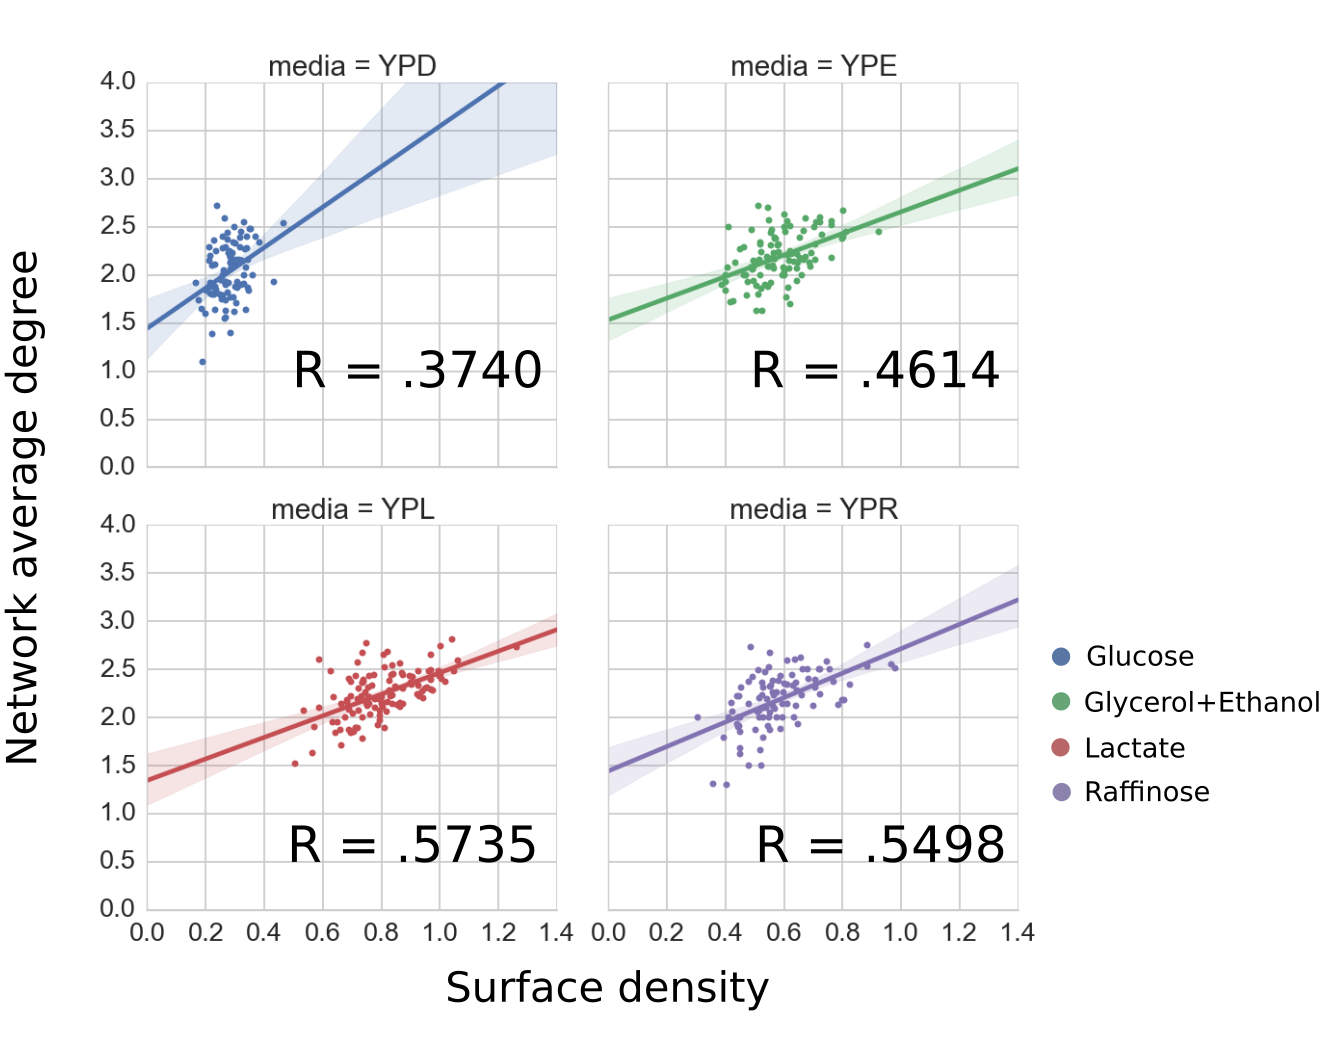
\includegraphics[width=.85\textwidth]{conndense}
    \caption[Network connectivity is positively correlated with mitochondrial surface density]{Network connectivity is positively correlated with mitochondrial surface density.\\Shown here is a plot of the network average degree with the mitochondrial surface density for each cell in different carbon sources. Cells in different carbon sources have different respiration rates which affect the surface density of mitochondria in the cell (\Fref{tab:params}). Mitochondrial networks grown in glucose undergo glucose repression and have the lowest surface density of mitochondria while those in non-fermentable (lactate, glycerol+ethanol) or non repressing fermentable carbon sources (raffinose) undergo aerobic respiration and have increased mitochondrial surface density. The connectivity of the network scales scales positively with the mitochondrial surface density because tubules in a dense mitochondrial network have a higher probability of encountering and forming connections with other tubules. The correlation holds true for other measures of global connectivity (\Fref{tab:glocon}).\\\emph{R value = Pearson correlation coefficient, $p$ value <0.05 that the Pearson correlation score is not significantly different from zero for all conditions.\\Number of cells---Glucose=96, Glycerol+Ethanol=111, Lactate=117, Raffinose=96.}}\label{fig:conndense}
\end{figure}
%
\subsection{Mitochondrial surface density scales with network connectivity}
The first question we address in analyzing functional heterogeneity at the mitochondrial network level is whether mitochondrial surface density and the connectivity of the network are related. In \Fref{fig:conndense} we plot the network average degree against the mitochondrial surface density for each cell in each of the four carbon sources (representing different respiratory conditions as described in \fref{sec:carbon}). The Pearson correlation coefficients show a significant positive correlation between mitochondrial surface density and the average degree of the network. Mitochondrial surface density also scales with other measures of global network connectivity as shown in \Fref{tab:glocon}. This suggest that mitochondrial tubules in cells with a dense mitochondrial network have a higher probability of forming connections with other tubules, simply by having a higher chance of encountering another tubule.
%
\begin{figure}[htp]
	\centering
    \hspace*{.75in}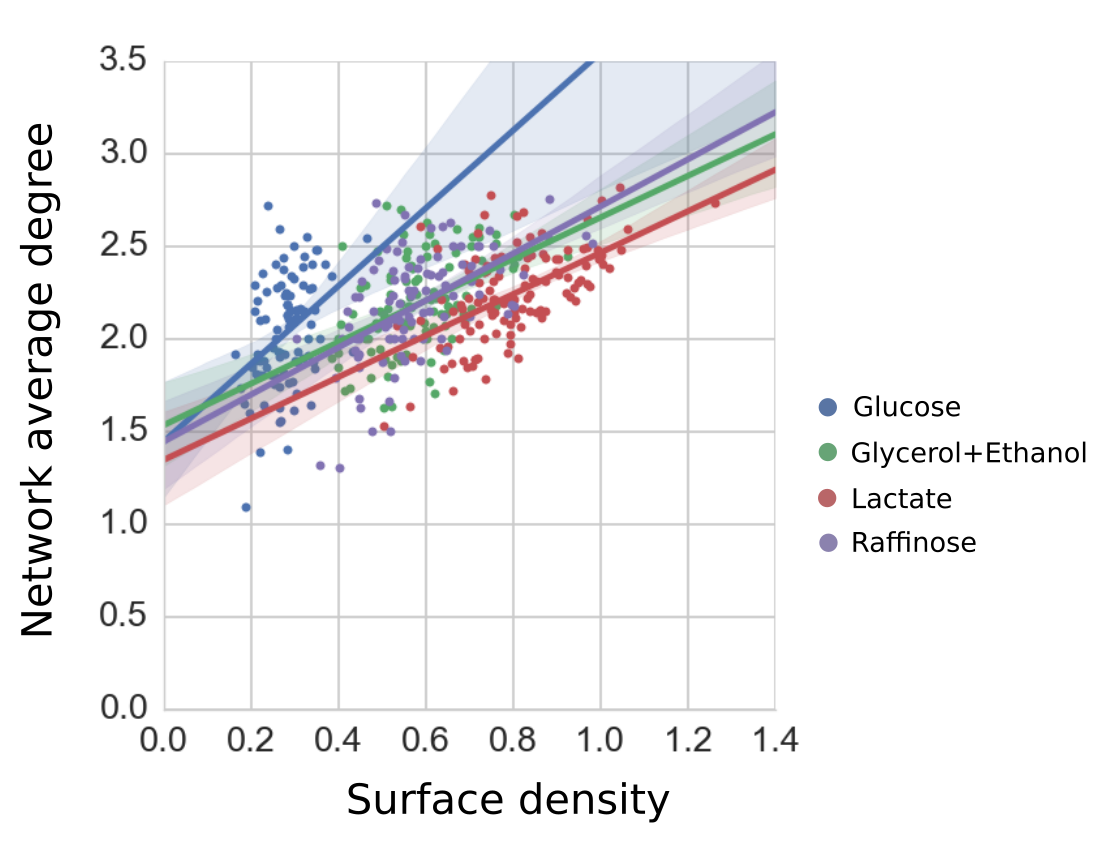
\includegraphics[width=.75\textwidth]{regbeta}
    \caption[Cells in fermentation have a higher regression coefficient for network connectivity--surface density ]{Cells in fermentation have a higher regression coefficient for network connectivity--surface density.\\Shown are the least square regression plots for the relationship between network average degree and surface density, for cells in different carbon sources. The respiration state (fermentation (glucose) or aerobic respiration (non-glucose)) affects the regression coefficient, $\beta$. For a given cell surface density, cells in fermentation display a higher network average degree.}\label{fig:regbeta}
\end{figure}
%

The correlation coefficients in \Fref{tab:glocon} only indicate how linear is the relationship between surface density and global connectivity. When the actual regressions were plotted (\Fref{fig:regbeta}), we see that cells in fermentation (glucose) display a steeper regression slope/coefficient ($\mitbeta$) compared to those in respiration (lactate, glycerol+ethanol, raffinose). This was true as well for the other global connectivity coefficients (not shown). We performed a statistical test on whether there was an interaction between the state of the cell (fermentation/respiration) and their regression coefficient for network average degree--surface density. This is a standard way to test if two different regression coefficients are the same \cite{jacoby_regression}. An interaction that is close to zero indicates that the regression coefficients between two populations are equal. The interaction term ('slope Density.:fermt[T.resp]', \Fref{tab:mytest}) is significantly different from zero ($\mitbeta_{\mathrm{respiration}}$ is -1.33 lower than $\mitbeta_{\mathrm{fermentation}}\,$, $p$ <0.01). Similar results were obtained when using different global connectivity measures (data not shown). This means that cells in fermentation display a higher connectivity for the same surface density compared to cells in respiration. This could indicate that connectivity is regulated in a respiration independent manner as cells in fermentation display network connectivity at a higher level then would be predicted by their surface density values alone (discussed in more detail in \fref{sec:discfive}).

The surface density does not show a strong correlation with measures of centrality or clustering coefficient (\Fref{tab:locon}). A high centrality score indicates the node is a 'hub', i.e. that node is at the intersection of many paths between other pairs of nodes. Our results suggest that nodes do not become more 'central' and the network does not become more of a 'hub-like architecture' as surface density increases.
\subsection{Mitochondrial surface density does not correlate with ΔΨ or connectivity}
We next investigate whether ΔΨ of the network correlates with network connectivity, as it has been observed that larger networks tend to have more fusion events \cite{jakobs_spatial_2003} which requires ΔΨ. Surprisingly we find that there is no correlation between the surface density of mitochondria with the mean cellular ΔΨ (the Pearson correlation coefficient between surface density and ΔΨ was not significantly different from zero, \Fref{fig:dydense}). We also investigated whether ΔΨ correlated with network connectivity (\Fref{tab:dyglo} and \Fref{tab:dylo}) and found no correlations that were significant. This means that a highly connected node (or region of nodes) does not have a different ΔΨ level compared to any other node.
%
\begin{figure}[htp]
	\centering
    \hspace*{.5in}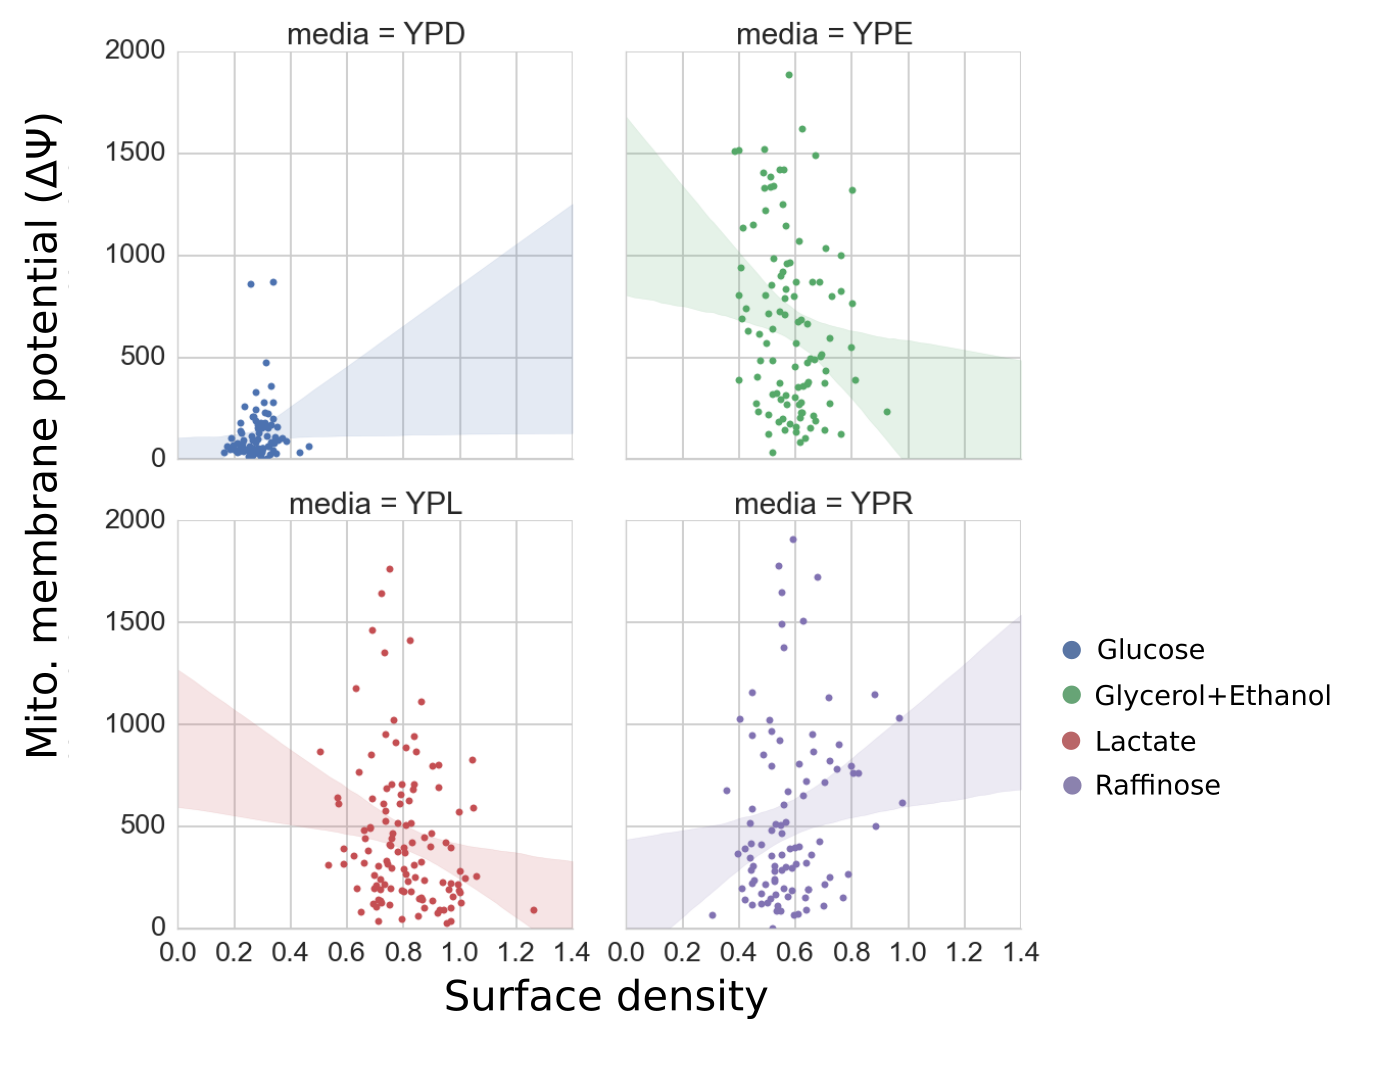
\includegraphics[width=.9\textwidth]{dydense}
    \caption[Mitochondrial membrane potential is not correlated with mitochondrial surface density]{Mitochondrial membrane potential is not correlated with mitochondrial surface density.\\Shown here is a plot between the mean mitochondrial membrane potential (ΔΨ) and mitochondrial surface density for each cell in different carbon sources (see \fref{sec:carbon} for details of the carbon sources). The $p$ value is >0.05, meaning that the Pearson correlation coefficient is not significantly different from zero for all conditions. There was also no clear correlation between ΔΨ and connectivity (\Fref{tab:dyglo} and \Fref{tab:dylo}). We conclude that cellular ΔΨ is independent of the surface density and connectivity of mitochondria in the cell. Changes in the respiration state (glucose vs the others) did not affect the lack of correlation between network connectivity and ΔΨ.}\label{fig:dydense}
\end{figure}
%
\subsection{Mitochondria with similar surface densities do not show a difference in correlation with ΔΨ or connectivity measures}
%
\begin{figure}[htp]
	\centering
    \hspace*{1.25in}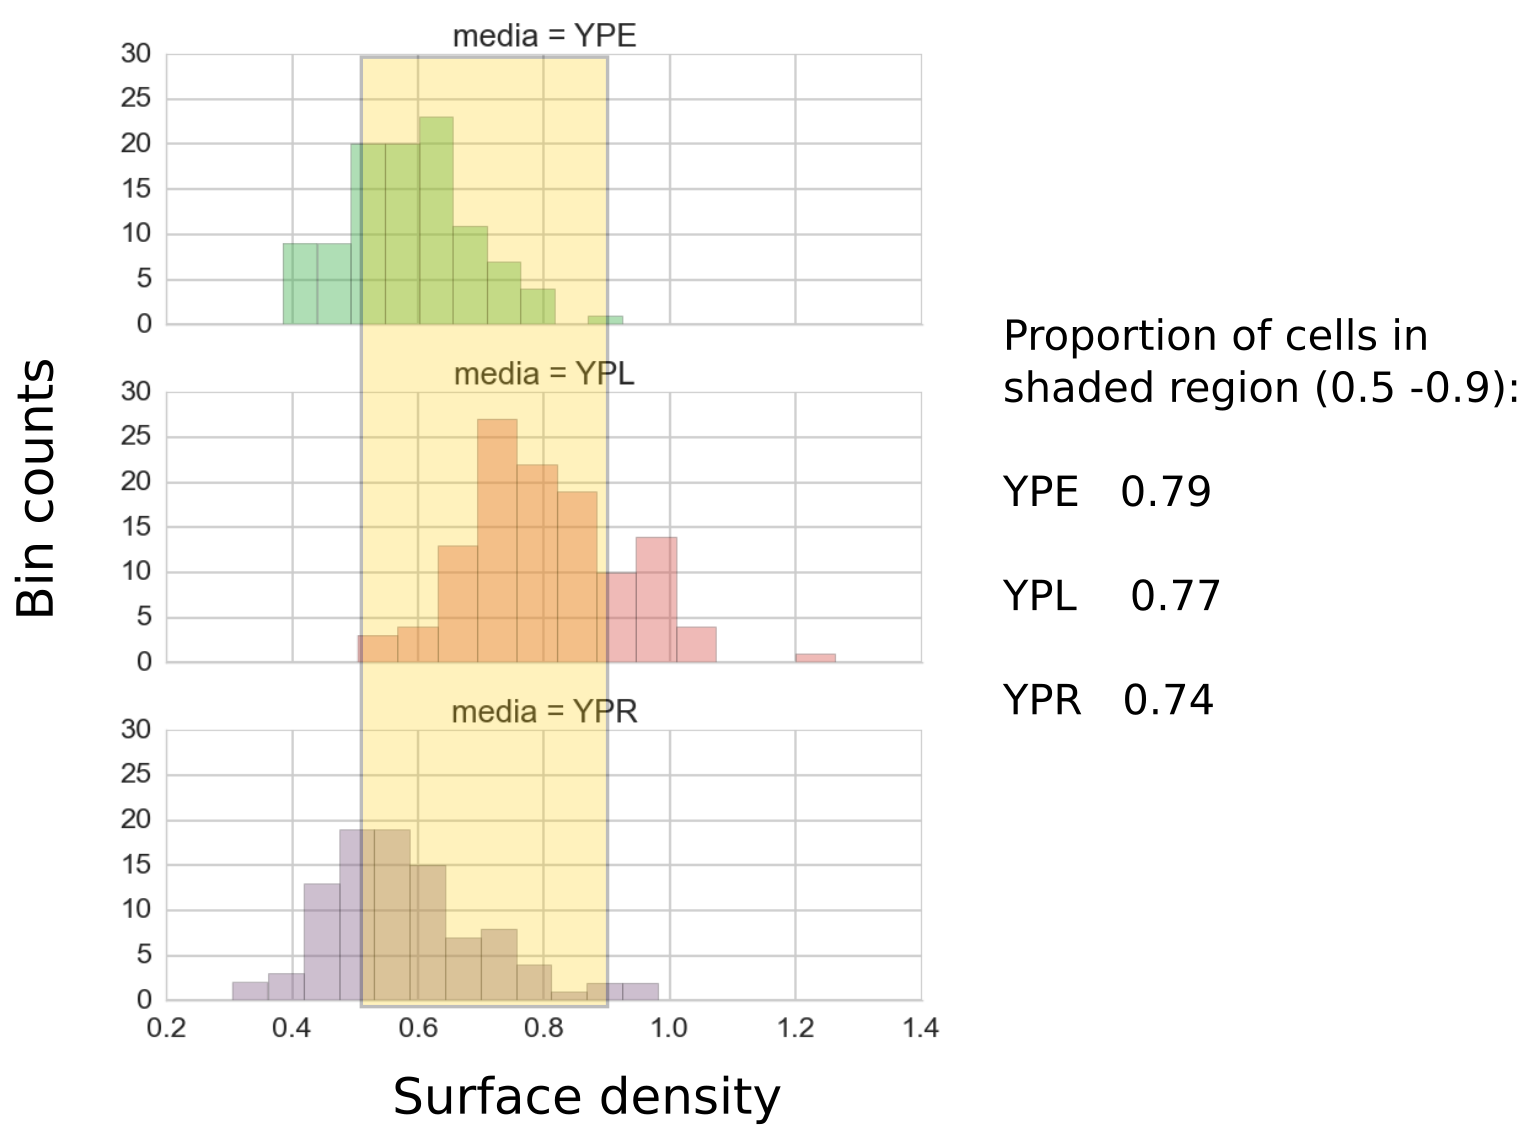
\includegraphics[width=.65\textwidth]{hist}
    \caption[Histogram of cell populations in respiratory conditions based on surface density]{Histogram of cell populations in respiratory conditions based on surface density.\\Variation in surface density in population of cells undergoing aerobic respiration might confound the analysis of ΔΨ with connectivity. To control for this, a subpopulation of the cells (shaded region) with surface density in the range 0.5--0.9 was selected to allow comparisons of ΔΨ and connectivity with similar surface densities of mitochondria. The size of the subpopulations was indicated as a proportion of the total number of cells in the full population.\\\emph{YPE = Glycerol+Ethanol, YPL = Lactate, YPR = Raffinose.}}\label{fig:hist}
\end{figure}
%
%
\begin{figure}[htp]
	\centering
    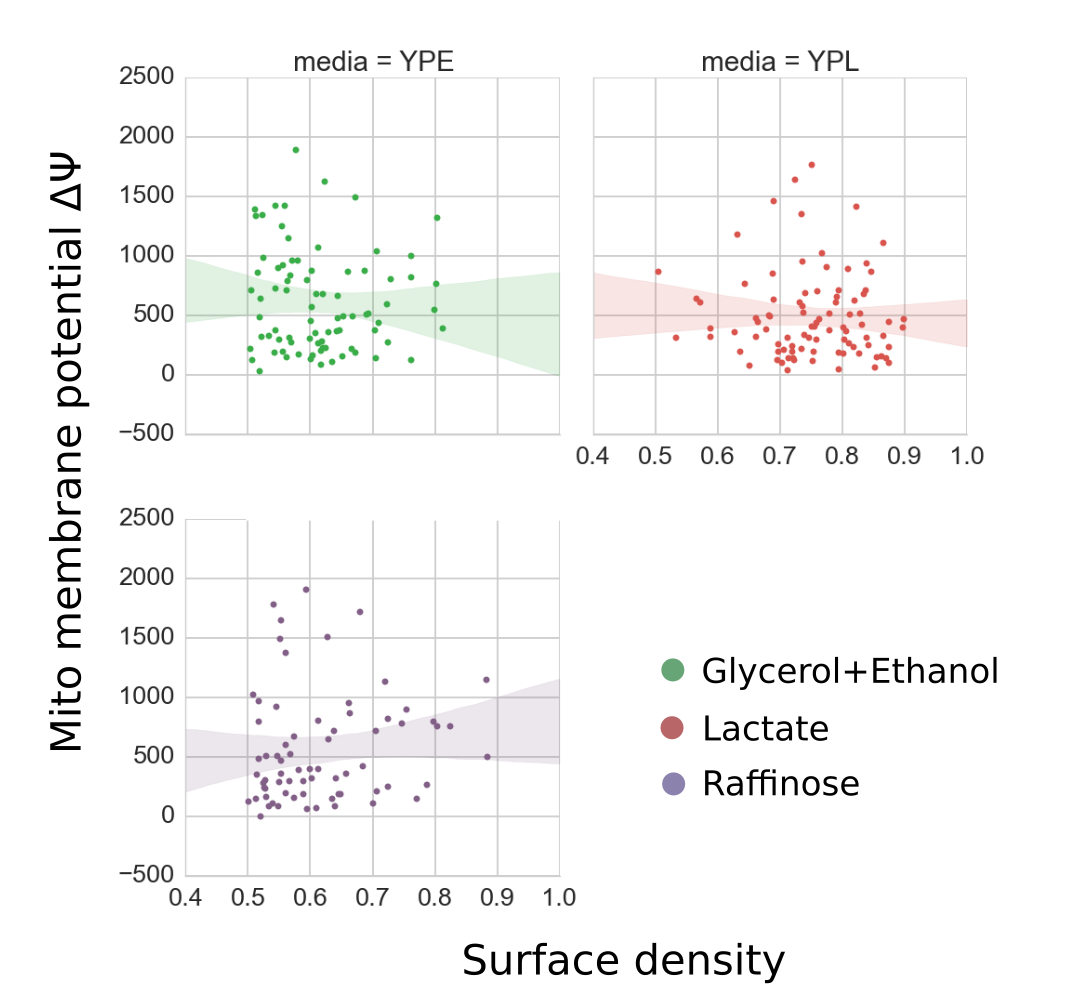
\includegraphics[width=.55\textwidth]{subset}
    \caption[Cells with similar surface density do not show correlation of with surface density]{Mitochondrial membrane potential is not correlated with surface density for subpopulation of cells with surface density in the range 0.5--0.9.\\After taking a subpopulation of cells with similar surface densities (\Fref{fig:hist}) for the three populations undergoing respiration, we found no correlation between ΔΨ and surface density. We also did not find significant correlations between ΔΨ and connectivity measures in the subpopulation (\Fref{tab:glosub}).}\label{fig:subset}
\end{figure}
%
A possible confounding factor when comparing connectivity vs ΔΨ of populations of cells grown in different carbon sources is that they display some variance in their surface density (\Fref{tab:params}). Since connectivity is affected by density, we have to ensure that we are comparing cell populations grown in carbon sources with similar surface densities of mitochondria in order to get a meaningful comparison. We decided to take a subpopulation of cells with a surface density in the range of 0.5--0.9 (\Fref{fig:hist}), ensuring that we had cells with a default higher amount of mitochondrial surface density. There were no cells from the glucose population (YPD) with surface density values in this range. As shown in (\Fref{fig:subset}) there was still no correlation between ΔΨ and mitochondrial surface density.
\subsection{Branchpoint regions have similar ΔΨ to non branchpoint regions}
%
\begin{figure}[htp]
	\centering
    \hspace*{.8in}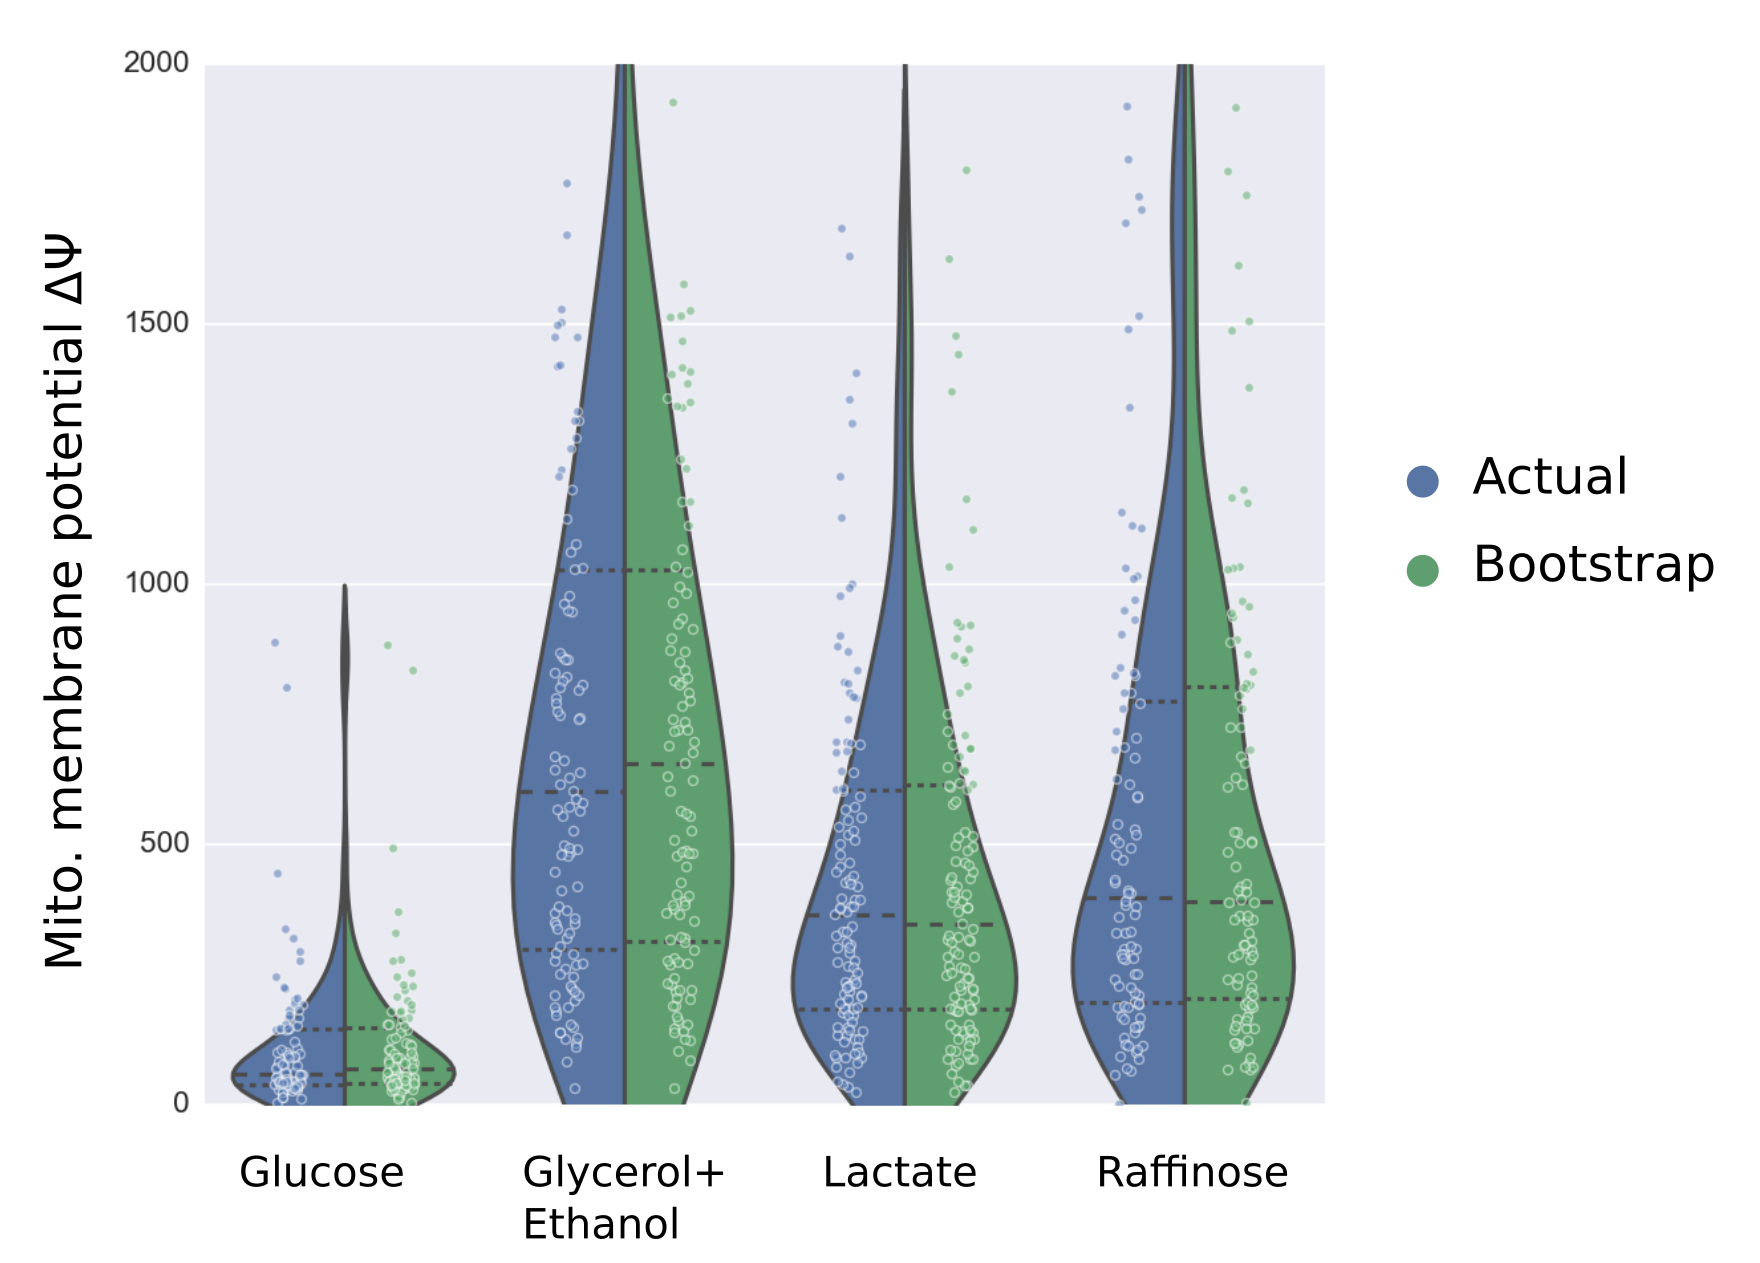
\includegraphics[width=.75\textwidth]{bpoints}
    \caption[Branchpoints do not show a difference in mean mitochondrial membrane potential (ΔΨ) compared to non branchpoints]{Branchpoints do not show a difference in mean mitochondrial membrane potential (ΔΨ) compared to non branchpoints.\\Shown here is the distribution of mean ΔΨ for each branchpoint (blue) or non branchpoint (green) for all mitochondrial networks in a population. To compare branchpoints ΔΨ and non branchpoints ΔΨ, a bootstrapped sampling of voxels that were not in the branchpoints regions was used to estimate the mean ΔΨ of non branchpoint regions. A branchpoint region was defined as a spherical region of radius 300nm centered at a node with degree of three or higher. The sampling population was equal to the number of branchpoints in that cell.\\\emph{Total number of branchpoints---Glucose=1134, Glycerol+Ethanol=1956, Lactate=3507, Raffinose=1623.}}\label{fig:bpoints}
\end{figure}
%
Since branchpoint regions are by definition sites of higher connectivity compared to the rest of the network, we investigated whether regions of mitochondrial tubules near a branching point (within a radius of \SI{300}{\nm}) had different ΔΨ levels compared to non branchpoint regions. We did this via a bootstrap sampling approach to compare branchpoints with equivalent samples of non branchpoints. The blue dots in \Fref{fig:bpoints} show the mean ΔΨ value of all branchpoints in a particular cell. For example for glucose where $N=96$ cells, there are 96 blue dots representing the mean ΔΨ of all branching points in each cell.

There are of course many fewer branchpoint regions compared to non branchpoint regions in a cell. To account for this, for each cell we sampled from the distribution of all non branchpoint voxels (defined as not lying within \SI{300}{\nm} of a branchpoint) in the mitochondrial network to construct a bootstrapped population of 'non-branchpoint' regions. The sampling population was equal to the number of branchpoints in that cell.
The mean of all the bootstrapped 'non-branchpoint' regions was then plotted as a green dot for the cell, and repeated for all cells in all populations (\Fref{fig:bpoints}). As can be seen from the violin plots in the figure, there was no difference in the distributions of ΔΨ between branchpoints and non branchpoints. Statistical testing performed as in \fref{sec:stat} also revealed no significant difference between the branchpoints and non branchpoints. Thus we conclude that branchpoints did not have a different ΔΨ level compared to non branchpoint regions.
\subsection{ΔΨ of isolated mitochondrial fragments are no different from the rest of the network }
%
\begin{figure}[htp]
	\centering
    \hspace*{.5in}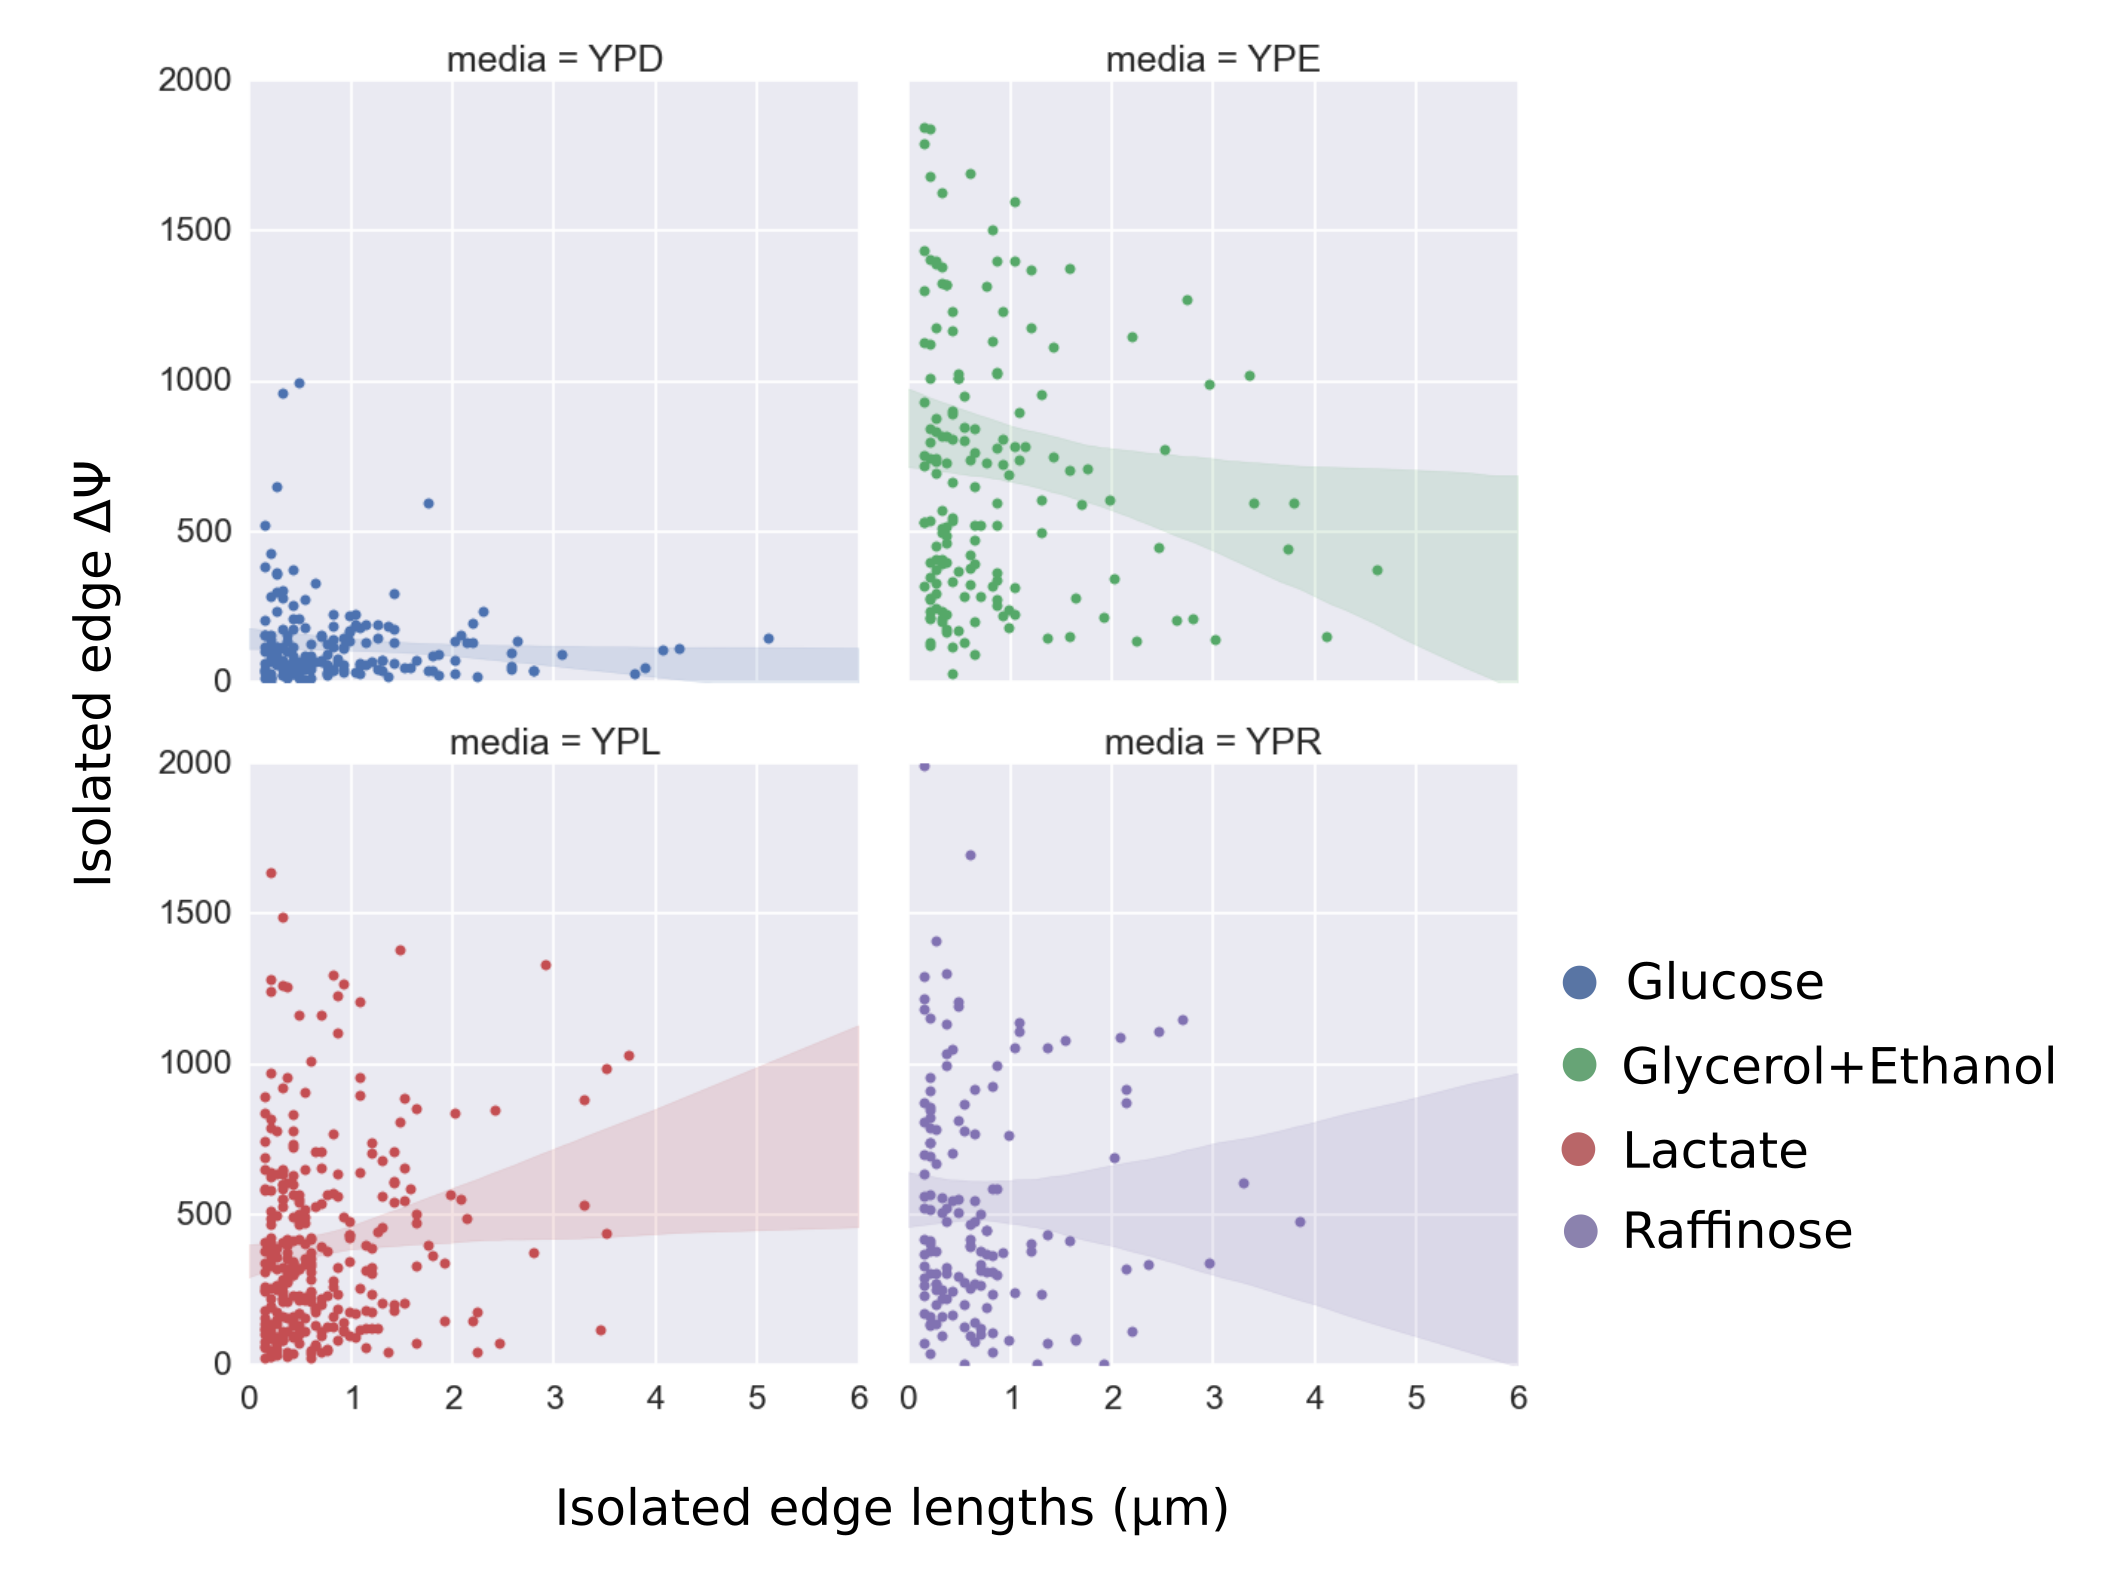
\includegraphics[width=.9\textwidth]{isoedges}
    \caption[Isolated mitochondrial fragments do not show a correlation of size with mitochondrial membrane potential]{Isolated mitochondrial fragments do not show a correlation of size with mitochondrial membrane potential.\\Shown here is plot of the mean ΔΨ vs length of all isolated mitochondrial tubules in each carbon source population. The lack of correlation between fragment ΔΨ and fragment length means that mitophagy selection does not depend on ΔΨ. Previous studies have shown that larger fragments are protected from mitophagy (\cite{rambold_tubular_2011}), hence if mitophagy selection was affected by ΔΨ it would be expected that the large fragments will have a higher overall ΔΨ, based on the assumption that healthier mitochondria are protected from mitophagy.\\\emph{Number of isolated fragments---Glucose=173, Glycerol+Ethanol=169, Lactate=305, Raffinose=148.}}\label{fig:isoedges}
\end{figure}
%
According to the mitochondrial quality control model, damaged mitochondria are targeted for mitophagy. It is also well known that mitophagy rate is correlated with mitochondrial length since small mitochondrial fragments are easier to be processed by the mitophagy machinery \cite{kanki_mitophagy_2008,rambold_tubular_2011}. We investigated whether isolated mitochondrial fragments with short lengths have a lower ΔΨ level, because we expected that on average any isolated fragments of mitochondria that were observed in the network would be those that have lower health/function and therefore be unable to fuse back to the network. We defined an isolated mitochondria in a network as a subgraph with only one edge. We found no correlation between ΔΨ and the length of the isolated mitochondria (\Fref{fig:isoedges}). Furthermore there was no clear clustering of short mitochondrial fragments in the low ΔΨ region, which would be observed if there was a 'threshold' level of functional fitness where short isolated mitochondria are targeted for mitophagy. In addition when we compared the ΔΨ of isolated fragments (regardless of their length) against the rest of the network, there was no difference in their mean ΔΨ (\Fref{fig:isorest}).
%
\begin{figure}[htp]
	\centering
    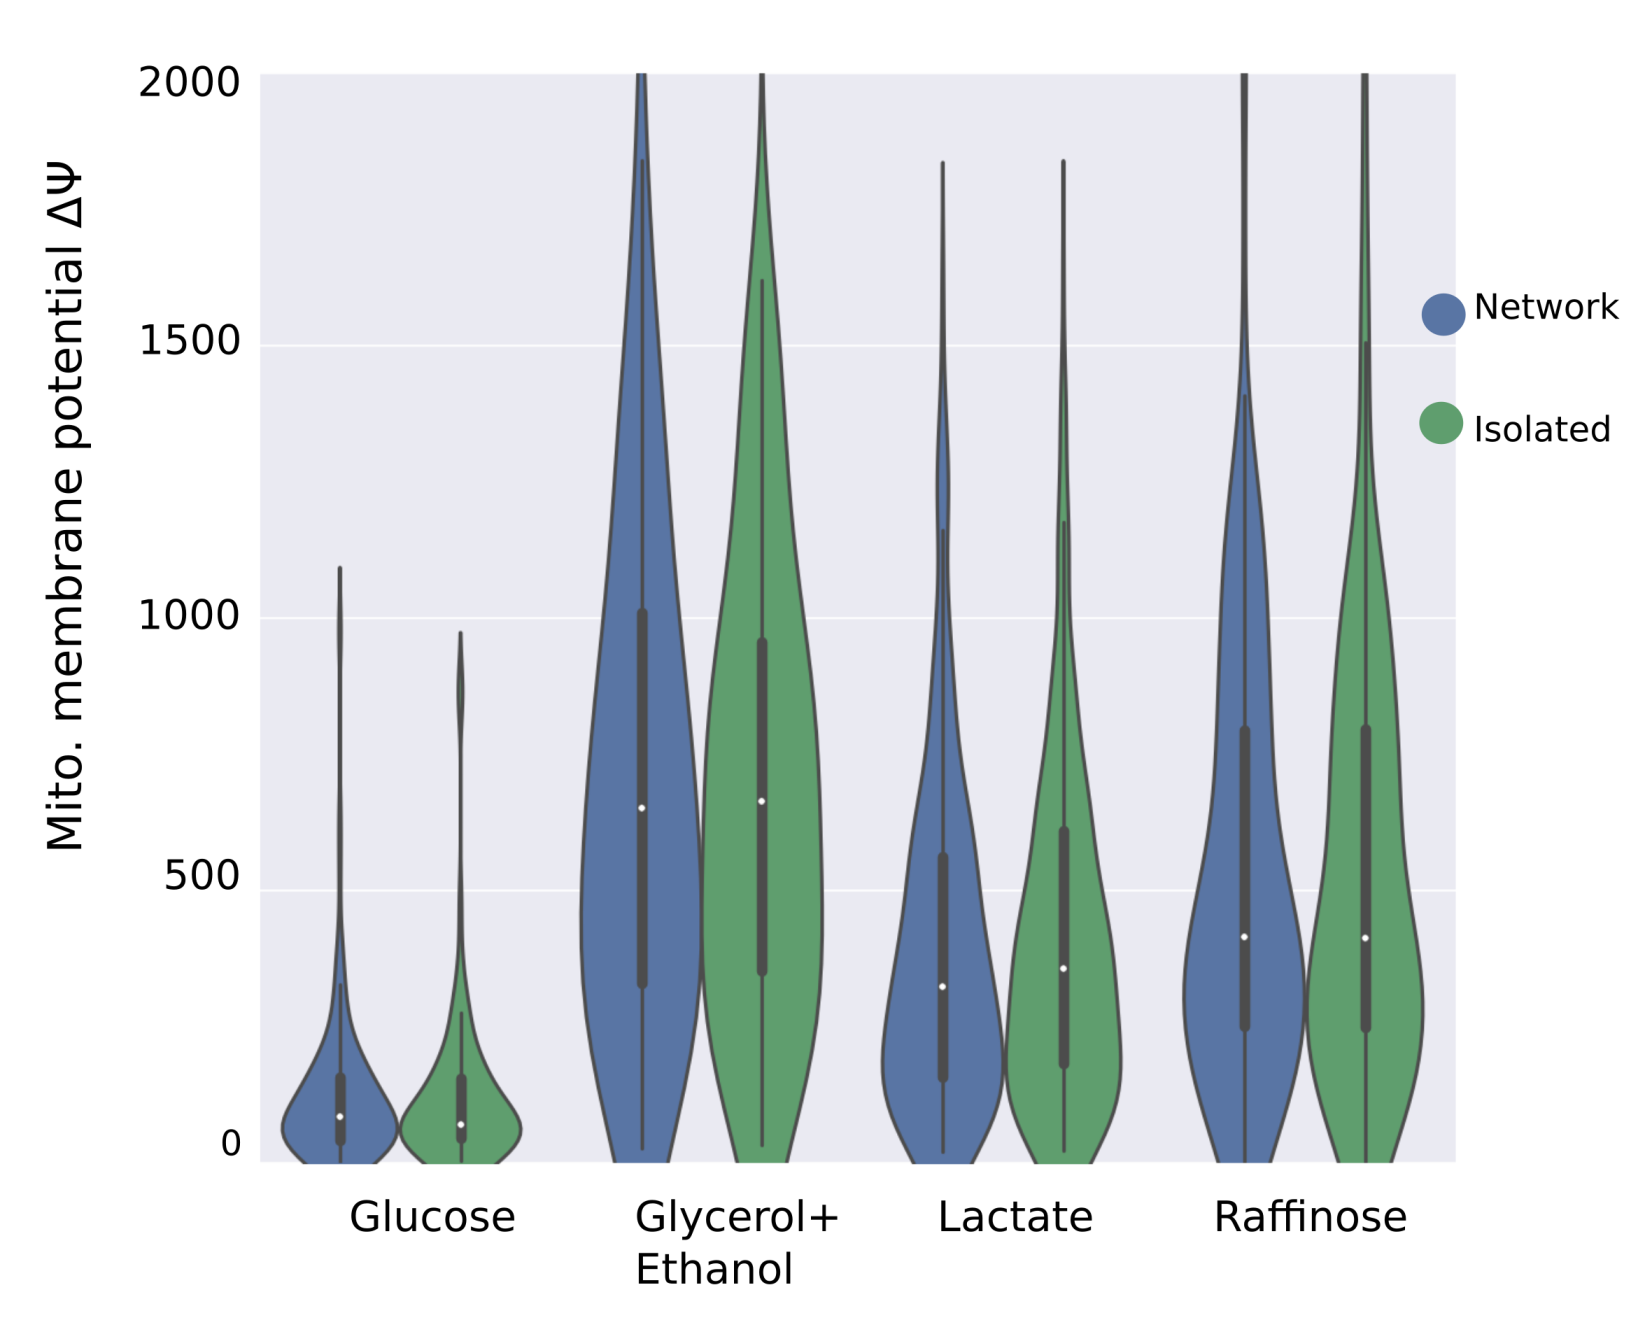
\includegraphics[width=.75\textwidth]{isorest}
    \caption[Isolated mitochondrial fragments do not show a difference in ΔΨ compared to the rest of the mitochondrial network]{Isolated mitochondrial fragments do not show a difference in ΔΨ compared to the rest of the mitochondrial network.\\Shown here is plot of the mean ΔΨ of isolated mitochondrial tubules (green) vs the rest of the connected network (blue) for each population of cells grown in different carbon sources. Isolated fragments do not show a any difference in their mean ΔΨ compared to the network of connected tubules.\\\emph{Number of isolated fragments---Glucose=173, Glycerol+Ethanol=169, Lactate=305, Raffinose=148.}}\label{fig:isorest}
\end{figure}
%

\section{Discussion}\label{sec:discfive}
We consistently found that cells with a higher density of mitochondria also have more connected mitochondrial networks. These results support the idea that mitochondrial tubules in a densely occupied cell surface would have a higher chance to encounter and fuse with another mitochondrial tubule. The three populations that undergo aerobic respiration (glycerol+ethanol, lactate and raffinose) also do not show a difference in their correlation of connectivity with surface density. Thus we conclude that the relationship between network connectivity and amount of mitochondria in the cell is independent of the carbon source as long as it undergoes respiration. Mitochondrial networks undergoing fermentation show a lower correlation between network connectivity and surface density. We found that mitochondrial networks in fermentation have a higher slope for the relationship between network connectivity and surface density. This means that cells in fermentation tend to form more connected networks at a given surface density value compared to those in respiration. As cells in fermentation have lower surface density (\Fref{tab:params}), it might be argued that this tendency for them to form more connected networks compared to respiring cells with the equivalent surface density is to reach a certain level of connectivity regardless of mitochondrial density. However this reasoning is complicated by the fact that cells in fermentation have a statistically significant lower overall connectivity level compared to those in respiration (see columns $\text{β}_{\V{geometric}}\,$, $\text{β}_{\V{topological}}\,$, φ, Pk$_3$ and average degree in \Fref{tab:params}, refer to \Fref{tab:tests} for the statistical test results). Nonetheless, our results imply that network connectivity is an essential feature of mitochondrial networks that is largely independent of respiration state. Results from our lab (data by M.Viana) indicate that one such role is to serve as a substrate to spread and mix mitochondrial content within the network. Simulations of fission/fusion protein mutants show that mitochondrial content mixing occur at a far slower rate compared to wild type cells. This is because wild type cells have network topologies with many more connections that can provide access to content mixing compared to fission/fusion mutants.

According to a model \cite{sukhorukov_emergence_2012} of the relationship between fusion/fission rates and the overall connectivity of the network, the probability $p$ of any two mitochondrial units to be connected are:
\begin{equation}
	\begin{split}
		\begin{aligned}
			&p=\frac{\text{α}_{\V{fusion}}}{\text{α}_{\V{fission}}+\text{α}_{\V{fusion}}} \\
			& \text{α}_{\V{fission}} \text{ and } \text{α}_{\V{fusion}} \text{ are the fission and fusion rates}
		\end{aligned}
	\end{split}
\end{equation}

Based on the model, above a critical value $p_c$ the network will be hyperfused (form a giant connected network with no tubules with free ends). As the global connectivity is higher in respiratory conditions, this implies that mitochondrial networks in respiratory conditions have higher fusion rate or lower fission rate. This suggests that respiration drives the fusion rate higher in order to increase mitochondrial surface density. An example of how fusion rate might be controlled is seen in the regulation of OPA1 processing in mammalian cells. It has been observed that OPA1 is targeted for increased proteolytic processing when ΔΨ is low \cite{ehses_regulation_2009}. This results in a lower overall fusion rate.

We found that ΔΨ did not correlate with either the surface density nor the connectivity of the network. This was surprising because cells with a higher respiration rate (and therefore increased mitochondrial amount) would be expected to have a high mitochondrial bioenergetic state. One possible explanation is that there is no selective fusion, hence no correlation between healthy/high ΔΨ mitochondria and dense/highly connected networks can be observed. However this conclusion goes against the dogma of mitochondrial quality control and would require much more direct evidence to prove this. Another possibility is that the selective fusion threshold is not based on ΔΨ but some other measure of mitochondrial function such as redox state or ROS levels. This hypothesis can be tested by adapting the pipeline described in \Fref{ch:two} to use biomarkers for redox or ROS levels \cite{mcfaline-figueroa_mitochondrial_2011}. The other possibility is that our assumption that highly connected regions were also the sites of higher mitochondrial fusion and fission activity is not true, at least at the global level. However there might still be localized areas of highly connected regions in the network that have higher fusion rates. This would require dynamic data (timelapse imaging) and an automated, reliable way to track fission and fusion sites. Work on this enhancement to MitoGraph is currently ongoing.

We also predicted that branchpoints, which are regions that have undergone fusion would be functionally different (in terms of ΔΨ). However our result indicating that there was no difference in ΔΨ between branchpoints and non branchpoints suggests that there is no functional difference. However without dynamic data we cannot distinguish which branchpoints have higher fusion activity and so cannot conclusively say that there is no functional difference in branchpoints. 

Lastly, we found it surprising that isolated fragments of mitochondria did not exhibit a lower level of ΔΨ. This is because the quality control model states that isolated mitochondria that are unable to fuse back to the network are targetted for mitophagy. Selective fusion means that these isolated fragment would on average be of lower ΔΨ. We further constrained our analysis to small fragments since mitophagy is known to size selective and still did not find a clear clustering of isolated mitochondrial fragments with lower ΔΨ. This suggest that there is no dependence on ΔΨ for mitophagy, which has been suggested in the literature \cite{hoitzing_what_2015}. However it is also possible that the isolated fragments we see are a mixture of fragments that have just undergone fission and have yet to fuse back. Thus we would need dynamic data to observe the mitochondrial fragments that undergo mitophagy and compare their ΔΨ just before undergoing mitophagy to conclusively determine whether mitophagy selects for lower ΔΨ fragments. Alternatively, we can create two populations with different mitophagy rates; a wild type population and a population with either a mitophagy impaired mutant \cite{kanki_atg32_2009} or one with increased fusion rate. In the mitophagy impaired mutant we expect the average ΔΨ to be lower than the wild type ΔΨ as there will be more unhealthy mitochondria in the population that is not mitophagized. Conversely in the population with increased fusion rates, we expect that there will be less unhealthy mitochondria in the population and hence a higher average ΔΨ compared to the wild type population.

In conclusion, we have determined that mitochondria form more connected networks when they are densely packed on the cell surface. However we could not find any evidence that these highly connected and densely packed networks have higher ΔΨ. We also could not find any functional difference in branchpoints or isolated mitochondrial fragments. Therefore we conclude that we will need dynamic data in order to resolve some of these surprising results.
\bigskip

\begin{table}[htp]
\sisetup{round-mode = places,round-precision = 3,table-format=3.3,table-space-text-post=1}
\centering
\caption[ΔΨ, global connectivity, local connectivity and surface density measures of mitochondrial networks in cells grown in various carbon sources.]{ΔΨ, global connectivity, local connectivity and surface density measures of mitochondrial networks in cells grown in various carbon sources.\\ $*\ p$<0.05 for the null hypothesis test that YPD is not significantly different from YPE, YPL and YPR, using rank sum test with multiple testing correction as detailed in \fref{sec:stat}. A list of tables for the statistical testing between conditions is included in the Appendix section (\Fref{tab:tests}).}
\footnotesize
\begin{tabular}{lSSSS}
\toprule
Carbon source &  {\parbox{1in}{\centering{ΔΨ (a.u.)}}} & \text{Surface Density}&$\text{β}_{\V{geometric}}$ & $\text{β}_{\V{topological}}$\\
\midrule
YPD (Glucose) & 114.2* &0.2812&0.6738* & 0.6842*\\
YPE (Ethanol +Glycerol) & 661.7 &0.5855&0.7851 & 0.7806\\
YPL (Lactate) & 443.5 & 0.8046&0.8099 & 0.8072\\
YPR (Raffinose) & 534.7 & 0.5812&0.7945 & 0.7970\\
\midrule
Carbon source & {\parbox{1in}{\centering{Pk$_3$}}}  & \text{Average degree} & {\parbox{1in}{\centering{Edge numbers}}}& {\parbox{1in}{\centering{φ}}} \\
\midrule
YPD (Glucose) & 0.4861* & 2.0352* & 24.7&0.6175*\\
YPE (Ethanol +Glycerol) & 0.5552 & 2.1903 & 34.4&0.7233\\
YPL (Lactate) & 0.5763 & 2.2466 & 58.2&0.7513\\
YPR (Raffinose) & 0.5567 & 2.1829 & 33.1&0.7422\\
\midrule
Carbon source & {\parbox{1in}{\centering{Betweenness centrality}}} & {\parbox{1in}{\centering{Near. neigh. degree}}} & {\parbox{1in}{\centering{Closeness centrality}}} & {\parbox{1in}{\centering{Clustering coefficient}}}\\
\midrule
YPD (Glucose) & 0.1149 & 2.3033* & 0.2165 &0.1163\\
YPE (Ethanol +Glycerol) & 0.1220 & 2.5151 & 0.2086&0.1053\\
YPL (Lactate) & 0.1027 & 2.6351 & 0.1559&0.0987\\
YPR (Raffinose) & 0.1355 & 2.5193 & 0.2125&0.1132\\
\bottomrule
\end{tabular}
\label{tab:params}
\end{table}
%

\begin{table}[htp]
\sisetup{round-mode = places,round-precision = 3,table-format=1.3,table-space-text-post=1}
\centering
\caption[Correlation of surface density with global connectivity]{Correlation of surface density with global connectivity.\\$p$<0.05 for all values in the table. The null hypothesis test was that the correlation coefficients were not significantly different from 0.}
\footnotesize
\begin{tabular}{p{2in}SSSS}
\toprule
Pearson correlation score of surface density with & \text{YPD} & \text{YPE} & \text{YPL}&\text{YPR}\\
\midrule 
Average degree & 0.3740 & 0.4614 & 0.5735&0.5498 \\ 
$\text{β}_{\V{geometric}}$& 0.3227 & 0.2607 & 0.4495&0.3803 \\ 
$\text{β}_{\V{topological}}$ & 0.2874 & 0.2864 & 0.4280&0.4126 \\ 
Edge numbers & 0.3665 & 0.3811 & 0.4846&0.5006 \\ 
\text{φ} & 0.3290 & 0.3302 & 0.4756&0.4551 \\ 
Pk$_3$ & 0.3889 & 0.4214 & 0.5856&0.5426 \\ 
\bottomrule
\end{tabular}
\label{tab:glocon}
\end{table}
%

\begin{table}[htp]
\sisetup{round-mode = places,round-precision = 3,table-format=1.3,table-space-text-post=1}
\centering
\caption[Correlation of surface density with local connectivity]{Correlation of surface density with local connectivity. \\$*\ p$<0.05 for the null hypothesis test that the correlation coefficients were not significantly different from 0.}
\footnotesize
\begin{tabular}{p{2in}SSS[table-format=-1.3,table-space-text-post=1]S}
\toprule
Pearson correlation score of surface density with & \text{YPD} & \text{YPE} & \text{YPL}&\text{YPR}\\
\midrule 
Average degree & 0.3740 & 0.4614 & 0.5735&0.5498 \\ 
Betweenness centrality & 0.2030 & 0.1171 & 0.2280&0.0787 \\ 
Closeness centrality & 0.0437 & 0.0576 & 0.1606&0.0749 \\ 
Clustering coefficient & 0.1575 & 0.0084 & -0.0315&0.1113 \\ 
Nearest neighbor degree & 0.4590* & 0.4559* & 0.5043*&0.5303* \\ 
\bottomrule
\end{tabular}
\label{tab:locon}
\end{table}
%

\begin{table}[htp]
\sisetup{round-mode = places,round-precision = 3,table-format=-1.3,table-space-text-post=1}
\centering
\caption[Correlation of ΔΨ with global connectivity and surface density]{Correlation of ΔΨ with global connectivity and surface density. No significant correlations were found.}
\footnotesize
\begin{tabular}{p{2in}SSSS}
\toprule
Pearson correlation score of ΔΨ with & \text{YPD} & \text{YPE} & \text{YPL}&\text{YPR}\\
\midrule 
Surface density & 0.1523 & -0.2319 & -0.2203&0.2058 \\ 
Average degree & -0.0430 & -0.0938 & 0.1193&0.0452 \\ 
$\text{β}_{\V{geometric}}$ & -0.0026 & -0.1545 & 0.0222&0.0591 \\ 
$\text{β}_{\V{topological}}$ & 0.0112 & -0.1147 & 0.0447&0.0605 \\ 
Edge numbers & 0.0260 & -0.1098 & -0.2652&-0.0831 \\ 
\text{φ}& -0.0073 & -0.0915 & 0.0606&0.0672 \\ 
\bottomrule
\end{tabular}
\label{tab:dyglo}
\end{table}
%

\begin{table}[htp]
\sisetup{round-mode = places,round-precision = 3,table-format=-1.3,table-space-text-post=1}
\centering
\caption[Correlation of ΔΨ with local connectivity]{Correlation of ΔΨ with local connectivity. No significant correlations were found.}
\footnotesize
\begin{tabular}{p{2in}SSS[table-format=1.3,table-space-text-post=1]S[table-format=1.3,table-space-text-post=1]}
\toprule
Pearson correlation score of ΔΨ with & \text{YPD} & \text{YPE} & \text{YPL}&\text{YPR}\\
\midrule 
Betweenness centrality & -0.0258 & -0.1214 & 0.0599&0.0801 \\ 
Closeness centrality & -0.0083 & 0.0001 & 0.2492&0.1567 \\ 
Clustering coefficient & 0.0233 & -0.1632 & 0.2467&0.0519 \\ 
Nearest neighbor degree & 0.0411 & 0.0133 & 0.0840&0.0044 \\ 
\bottomrule
\end{tabular}
\label{tab:dylo}
\end{table}
%

\begin{table}[htp]
\sisetup{round-mode = places,round-precision = 3,table-format=1.3,table-space-text-post=1}
\centering
\caption[Correlation of surface density with global connectivity for the subpopulation of cells with surface density in the range 0.5--0.9]{Correlation of surface density with global connectivity for the subpopulation of cells with surface density in the range 0.5--0.9.\\$*\ p$<0.05 for the null hypothesis test that the correlation coefficients were not significantly different from 0.}
\footnotesize
\begin{tabular}{p{2in}S[table-format=2.0]SSS}
\toprule
Pearson correlation score of surface density with & \text{YPD} & \text{YPE} & \text{YPL}&\text{YPR}\\
\midrule 
Average degree & NA & 0.3816* & 0.4217*&0.4419* \\ 
$\text{β}_{\V{geometric}}$& NA & 0.0873 & 0.3926*&0.3123*\\ 
$\text{β}_{\V{topological}}$ & NA & 0.0896 & 0.3514*&0.3564* \\ 
Edge numbers & NA & 0.3066* & 0.4571*&0.3198*\\ 
\text{φ} & NA & 0.1203 & 0.3595*&0.3880*\\ 
Pk$_3$ & NA & 0.3117* & 0.4421*&0.4190* \\ 
\bottomrule
\end{tabular}
\label{tab:glosub}
\end{table}
%

\begin{table}[htp]
\sisetup{round-mode = places,round-precision = 3,table-format=-1.3,table-space-text-post=1}
\centering
\caption[Correlation of surface density with local connectivity for the subpopulation of cells with surface density in the range 0.5--0.9]{Correlation of surface density with local connectivity for the subpopulation of cells with surface density in the range 0.5--0.9.\\$*\ p$<0.05 for the null hypothesis test that the correlation coefficients were not significantly different from 0.}
\footnotesize
\begin{tabular}{p{2in}S[table-format=2.0]SSS[table-format=1.3,table-space-text-post=1]}
\toprule
Pearson correlation score of surface density with & \text{YPD} & \text{YPE} & \text{YPL}&\text{YPR}\\
\midrule 
Betweenness centrality & NA & -0.0179 & 0.2081*&0.0569 \\ 
Closeness centrality & NA & -0.0161 & 0.0190&0.1102 \\ 
Clustering coefficient & NA & 0.1367 & -0.0097&0.0808 \\ 
Nearest neighbor degree & NA & 0.3955* & 0.4003*&0.4978*\\ 
\bottomrule
\end{tabular}
\label{tab:losub}
\end{table}

















\chapter[Membrane potential heterogeneity at the cellular level]{Membrane potential heterogeneity at the cellular level: mother-bud asymmetry of mitochondrial function in budding yeast}\label{ch:six}
\clearpage
\section{Introduction}
Eukaryotic cells exhibit cell polarity, i.e. spatial heterogeneity in the structure and function of cellular components such as the cytoskeleton, organelles and cell surfaces. Cell polarity results from asymmetric distribution and organization of cellular components and function within the cell. Well known examples are the apical and basolateral plasma membrane domains in epithelial cells and the dendrite and axon terminals seen at the synapses of neurons. The life cycle of organisms exhibit polarity in the form of asymmetric cell division. Young individuals are born with low levels of damaged proteins that is mostly independent of the age of their parents. This is thought to be crucial to maintain healthy germline cells at the expense of somatic cells ('disposable soma theory', \cite{kirkwood_evolution_1979}.

Budding yeast experience polarized cell growth at several stages during its life cycle. For example haploid cells exposed to a pheromone from another cell of the opposite mating type arrest cell growth in G1 and form projections towards the other cell \cite{madden_cell_1998}. While mating is a distinct transition in the life cycle of budding yeast, for this thesis we are only interested in their mitotic life cycle. Budding yeast cells undergo cell proliferation where the original mother cell gives rise to a bud/daughter cell with an entirely new cell surface. While budding yeast does not have a germline/somatic cell distinction, they do display age related changes in cellular function and fitness. Mother cells do not divide forever, they stop after around 20--25 divisions and then enter a short postreplicative state before lysis \cite{longo_replicative_2012}. The number of times the mother cell can divide is known as its replicative life span. As it ages, the mother cell exhibits accumulation of oxidatively damaged proteins and extrachromosomal rDNA circles \cite{aguilaniu_asymmetric_2003}, impaired mitochondria \cite{lai_mutation_2002} and eventually loses the ability to undergo further cell division \cite{laun_aged_2001}. However daughter cells are born with full replicative potential \cite{steinkraus_replicative_2008} and much lower levels of oxidative stress \cite{aguilaniu_asymmetric_2003}. Oxidative damage is thought to contribute to age related decline in mitochondrial and cellular function \cite{huang_role_2004,lai_mutation_2002}.

There is emerging evidence for the existence of a mitochondrial quality control mechanism via fission and fusion to segregate healthy mitochondria and that buds preferentially inherit these mitochondria during cell division \cite{klinger_quantitation_2010,mcfaline-figueroa_mitochondrial_2011}. An early study noted a reduced level of mitochondrial membrane potential (ΔΨ) in older populations of budding yeast cells using flow cytometry \cite{lai_mutation_2002}. This study was done using a method that lacks single cell resolution level, and hence cannot answer how functional asymmetry is distributed within the cell. A study by Pon et al. \cite{mcfaline-figueroa_mitochondrial_2011} showed evidence of an intracellular asymmetry of function in budding yeast at single cell resolution level. They quantified levels of oxidative redox potential using a mitochondrial matrix targeted fluorescent protein marker (roGFP1) and also superoxide levels by staining with dihydroethidium (DHE). They found that mother cells retained mitochondria with a lower ratio of reduced to oxidized roGFP1 and higher superoxide levels compared to buds. They also showed that the ratio of reduced to oxidized roGFP1 in mother and bud cells decreased with replicative age, meaning that mitochondria in old cells were more oxidized .

What the above studies lacked was that there was no analysis of the spatial distribution of function in mitochondrial networks along the mother-bud cell axis. This means that previous studies did not quantify the distribution of a functional marker at specific regions along this axis that might be important to the cell cycle. For example, the bud neck is believed to be a bottleneck for movement of all cargoes into the bud \cite{vevea_inheritance_2014} and it would be interesting therefore to see if mitochondrial quality around this region could impact bud growth. Using the methods developed in \Fref{ch:two}, we extended the analysis of functional heterogeneity of mitochondria at the cellular level using the distribution of ΔΨ along an axis that represents the polarity of the mother-bud cell axis. We show for the first time how ΔΨ is distributed along this axis and provides a quantitative analysis of how this ΔΨ distribution varies with budding progression.
\section{Materials and Methods}
\subsection{Picking of points to define the mother-bud axis}
We used the open-source Mayavi 3D visualization software (\url{http://code.enthought.com/projects/mayavi/}) to render in 3D the mitochondrial network skeleton based on the outputs from MitoGraph v2.0. Mayavi has convenient function wrappers in Python for handling VTK objects and makes it easier to write interactive software for the cell picking procedures described below.

The cell surfaces (yellow ellipses) shown in \Fref{fig:coors} were drawn using the Mayavi's Parametric Surface function. The major and minor axis length, center coordinate and angle of the ellipse was obtained via an ImageJ ellipse fit of a hand traced ROI of the brightfield data of the actual cell, as detailed in \fref{sec:ROI}. The surfaces shown represent the 3D rendering of that ellipse fit. Additionally, it was often necessary to center the cell surfaces in the $z-$axis. This was because the focal slice position used to trace the brightfield image was often not aligned with the $z-$axis midpoint of the mitochondrial skeleton (which is based on MitoGraph v2.0's coordinate outputs). This would often result in the skeleton 'jutting out' in the $z-$axis from the cell surface (\Fref{fig:caveatA}). Centering was done via another mouse callback function by iteratively picking a position in the skeleton (magenta dot in the figure) that resulted in full enclosure of the skeleton by the cell surface.

To define the mother-bud axis, we picked three points; the base, tip and neck points on the cell surfaces via a mouse callback function (a function invoked when a mouse button was pressed). The base and tip represent the ends of the cell surfaces on the mother side and the bud side respectively. For the picking of the neck point, the intersection between mother and bud was estimated by taking the mid point of the intersection between the mother and bud surfaces (\Fref{fig:caveatB}). Care was also taken to pick the extreme ends of the cell surface and not the skeleton (\Fref{fig:caveatC}, blue and green dots). This was important because the mitochondrial skeleton was not always fully distributed at the ends of the cell surface, especially in cells with low amount density of mitochondria. Picking the points on the surface allows us to obtain correct correct localization of the mother-bud axis.
%
\begin{figure}[htp]
	\centering
    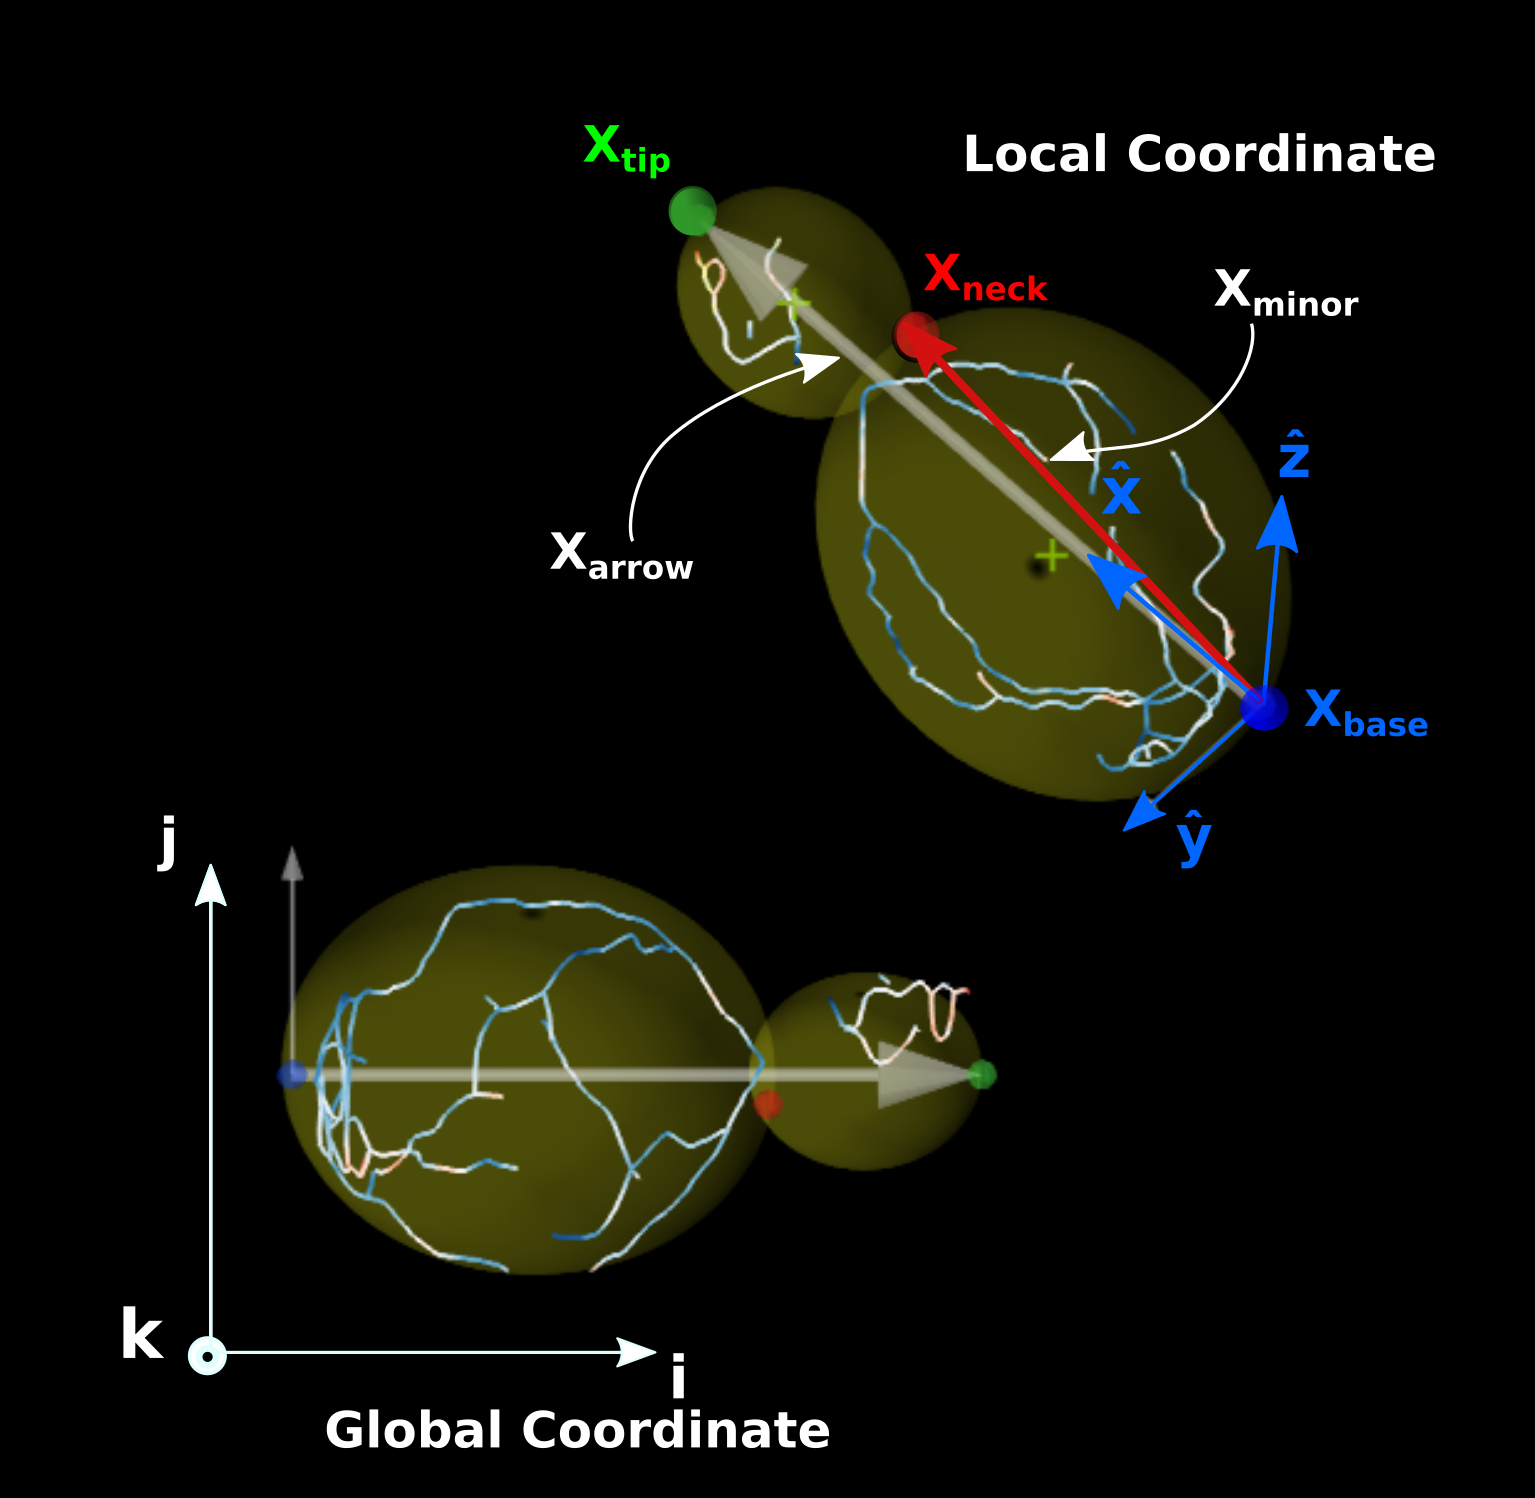
\includegraphics[width=.8\textwidth]{coors}
    \caption[Global and local coordinate system]{Global and local coordinate system.\\Shown in this figure is a mitochondrial network and cell that will be transformed from its original orientation in the 'Local Coordinate' to the 'Global Coordinate' system based on the Cartesian coordinate system with origin at $(0,0,0)$. The yellow ellipse surfaces represent the cortical periphery of the cell, with a mother (larger ellipse) and bud (smaller ellipse). The large arrow ($\mathbf{X_{arrow}}$) represents the mother-bud cell axis. A mouse callback routine written in Mayavi/Python was used to transform the cell by picking three points (blue,red and green). The blue and green points define the orientation of  $\mathbf{X_{arrow}}$. In order to constrain the rotation plane, a third point was needed and is represented by the red point. The location of the red point was chosen as the intersection between the mother and bud cell surfaces. The red arrow represents a position vector for this intersection (called the bud neck) and is coplanar with the $x-y$ plane of the local coordinate system. The transformation matrix translates and rotates the entire skeleton/cell so that the local $x-y$ plane lies on the global $x-y$ plane. The translation is based on the location of the blue point ( $\mathbf{X_{base}}$) so that after transformation the blue point lies on the origin $(0,0,0)$ of the global coordinate system.}\label{fig:coors}
\end{figure}
% 
%
\begin{figure}[htp]
	\centering
    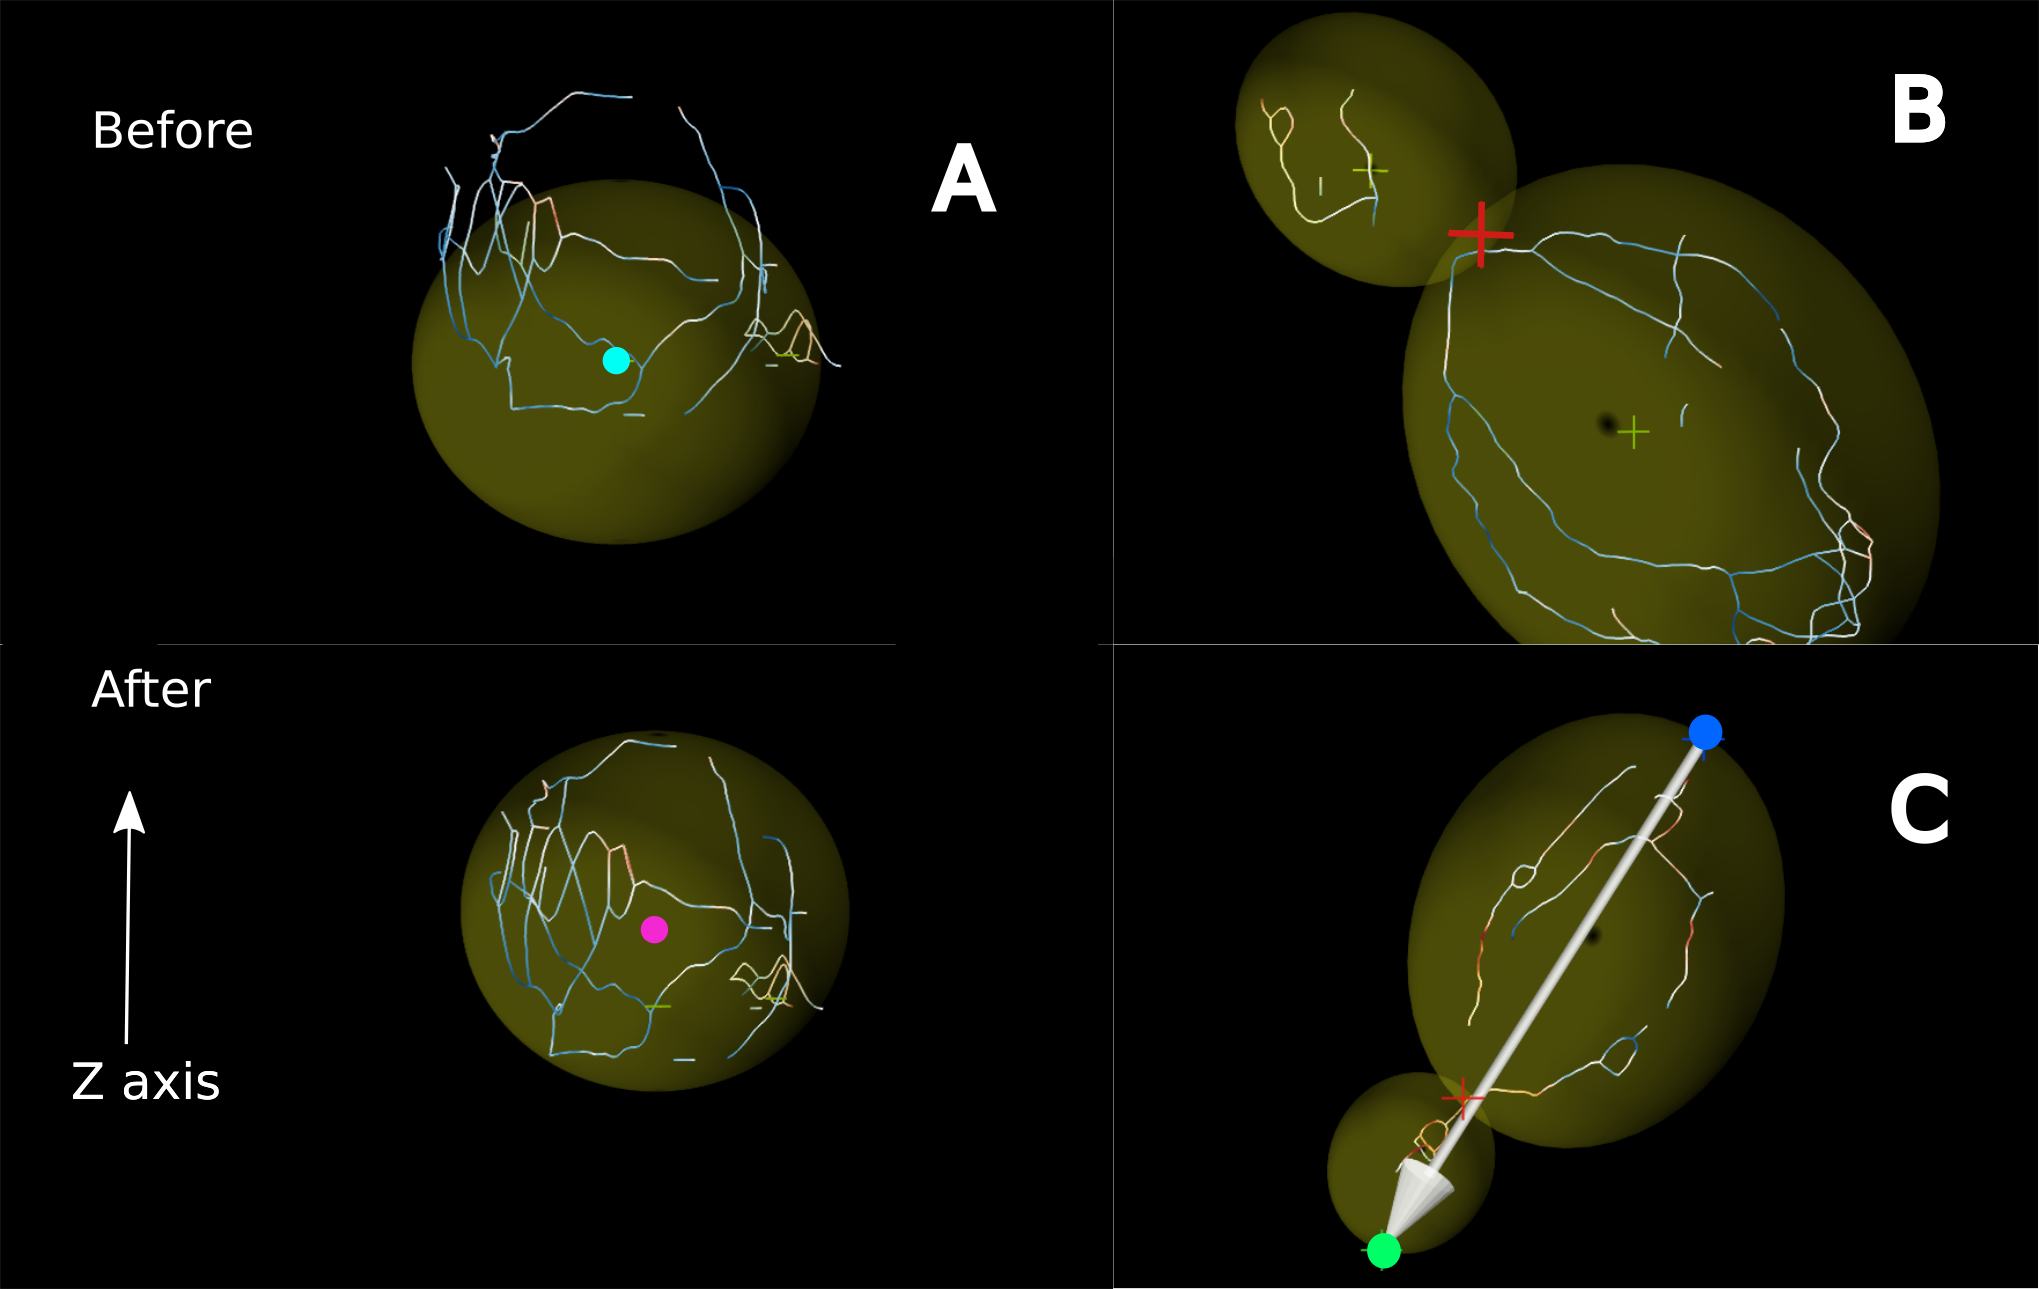
\includegraphics[width=.9\textwidth]{caveat}
     \subcaptionbox{An example of a skeleton that is not aligned with the cell surface (represented by the yellow ellipse, with the ellipse center shown in cyan). The cell surface was based on an ellipse fit of a hand traced outline of the inflection point in the $z-$position of the original brightfield image. The inflection point is the frame with the least visible outline of the cells in the brightfield image stack. A mouse callback function was used to pick the magenta point which repositions the cell surface so that it had good alignment with the skeleton.\label{fig:caveatA}}[\linewidth]{}
      \subcaptionbox{The bud neck region was picked based on the intersection of the two cell surfaces and is represented by the red cross. The bud neck coordinate is used to partition the cell into a mother and bud region.\label{fig:caveatB}}[\linewidth]{}
       \subcaptionbox{Care was always taken to pick the boundary of the cell based on the cortical periphery of the cell surface and not the skeleton. In this case the blue and green points were chosen to represent the base (blue) and tip (green) of the mother-bud cell axis.\label{fig:caveatC}}[\linewidth]{}
    \caption{Caveats when picking transformation points.}\label{fig:caveat}
\end{figure}
%
\subsection{Direction cosine based transformation matrix to realign the mother-bud cellular axis}
In order to analyze mother-bud functional asymmetry, it is necessary to define a coordinate system that conveniently aligns with the mother-bud cell axis. 
The direction cosine matrix is a matrix containing the cosines of the angle between a vector and its basis. It is used to express a vector in one orthogonal basis to a different basis \cite{kane_spacecraft_1983}. It can be used to transform the coordinates of all points in the mitochondrial skeleton so that for example, the mother-bud axis aligns parallel with the $x-$axis unit vector $(1\Vi+0\Vj+0\Vk)$. The transformation matrix $\mathbf{T}$ is given by:
\begin{equation}
	\begin{split}
		\begin{aligned}
			\mathbf{X_{global}} &= \mathbf{T X_{local}} \\
			%
			\mathbf{X_{global}} &= \text{vector coordinates expressed with basis } \mathbf{i,j,k} \\[-1.5ex]
			&\qquad\text{of the Cartesian coordinate system} \\
			%
			\mathbf{X_{local}} &= \text{vector coordinates expressed with basis } \mathbf{x,y,z} \\[-1.5ex]
			&\qquad\text{of the Cartesian coordinate system} 
		\end{aligned}
	\end{split}
\end{equation}
Suppose we want to transform the coordinates of all the points in the skeleton in \Fref{fig:coors} ('Local coordinate'). To define the mother-bud axis we pick two points represented by the blue and green dots. The blue and green dots represent the base and tip respectively of the mother-bud cell periphery. The mother-bud axis will be the main axis, and for convenience we define it as the $x-$axis of the local coordinate system. We need to pick another point to fix the plane of rotation, which we define as the plane formed by the blue (base), green (tip) and red (neck) dots and call this plane the $x-y$ plane in the local coordinate system. Therefore the three dots can be expressed as position vectors in the Cartesian coordinate system:
\begin{equation}
\begin{split}
		\begin{aligned}
		   \mathbf{X_{base}}&=X_{base}\Vi+Y_{base}\Vj+Z_{base}\Vk\\
		   \mathbf{X_{tip}}&=X_{tip}\Vi+Y_{tip}\Vj+Z_{tip}\Vk\\
		   \mathbf{X_{neck}}&=X_{neck}\Vi+Y_{neck}\Vj+Z_{neck}\Vk\\
		\end{aligned}
	\end{split}
\end{equation}
Consider a vector $\mathbf{X_{arrow}}$ represented by the large, white arrow in \Fref{fig:coors} ('Local coordinate') which represents the mother-bud axis. In the local coordinate system it has unit vectors $\xhat,\yhat,\zhat$:
\begin{equation}\label{eq:TM}
 	\begin{split}
	 	\begin{aligned}
	 		\mathbf{T}&=\begin{bmatrix}
			 		x_{1} &x_{2}&x_{3}&X_{base}\\
			 		y_{1} &y_{2}&y_{3}&Y_{base}\\
			 		z_{1} &z_{2}&z_{3}&Z_{base}\\
			 		0&0&0&1
		 		\end{bmatrix}		\\
		 	x_{1}, y_{1}, z_{1}\text{ are the direction } &\text{cosines of the x-axis in the local coord. system}\\[-1.5ex]
			x_{2}, y_{2}, z_{2}\text{ are the direction } &\text{cosines of the y-axis in the local coord. system}\\[-1.5ex]
			x_{3}, y_{3}, z_{3}\text{ are the direction } &\text{cosines of the z-axis in the local coord. system}
		\end{aligned}
	\end{split}
\end{equation}
The matrix formed by the direction cosines in \eqref{eq:TM} is the rotation matrix to rotate from the Cartesian to the local coordinate system, and the last column vector represents a translation from the origin $(0,0,0)$ to the position at $\mathbf{X_{base}}$.
The $(x_1, y_1, z_1)$ direction cosines of the vector $\mathbf{X_{arrow}}$, which has unit vector $\xhat$ is:
\begin{equation}\label{eq:dcosine}
	x_{1}= \frac{X_{tip}-X_{base}} {|X_{arrow}|} \quad x_{2}= \frac{Y_{tip}-Y_{base}} {|X_{arrow}|} \quad x_{3}= \frac{Z_{tip}-Z_{base}} {|X_{arrow}|}
\end{equation}
The direction cosines $(t_1, t_2, t_3)$ for $\mathbf{X_{minor}}$ can be found in the same manner as in equation \eqref{eq:dcosine} by replacing $\mathbf{X_{tip}}$ with $\mathbf{X_{neck}}$. 
Now, because the vectors $\mathbf{X_{arrow}}$ and $\mathbf{X_{minor}}$ (red arrow in \Fref{fig:coors}) formed by the three coplanar points $\mathbf{X_{base}}$, $\mathbf{X_{neck}}$ and $\mathbf{X_{tip}}$  lie on the $x-y$ plane of the local coordinate system, the unit vector $\zhat$ is orthogonal to this $x-y$ plane (i.e. the dot product of the vectors is zero):
\begin{align}
\mathbf{\hat{z_{base}}}\cdot \mathbf{X_{arrow}} &= x_3x_1+y_3y_1+z_3z_1=0 \nonumber \\
\mathbf{\hat{z_{base}}}\cdot \mathbf{X_{minor}} &= x_3t_1+x_3t_2+z_3t_3=0
\end{align}
Expressing $x_3$ and $y_3$ in terms of $z_3$ and using the unit vector definition of $\mathbf{Z_{base}}$ we obtain the $(x_3, y_3, z_3)$ components of the unit vector $\zhat$:
\begin{equation}
 	\begin{split}
	 	\begin{aligned}
	 		\zhat &= \frac {x_3\Vi+y_3\Vj+z_3\Vk}{\sqrt{x_3^2+y_3^3+z_3^2}}\\[1ex]
	 		\zhat &= \frac{x_3}{D}\Vi+\frac{y_3}{D}\Vj+\frac{z_3}{D}\Vk \\[1ex]
	 		\text{where D}&= \sqrt{\left(\frac{t_3}{t_1+t_2}\right)^2 +\left( \frac{t_3 x_1-t_1 z_1-t_2 z_1}{t_1 y_1+t_2 y_2}\right)^2+1}
		\end{aligned}
	\end{split}
\end{equation}	 	
Then obtaining the $(x_2, y_2, z_2)$ components of the unit vector $\yhat$ is done by taking the cross product of the other two orthogonal unit vectors:
\begin{equation}
\yhat=\zhat\times\xhat
\end{equation}
The transformation matrix to transform the cell so that the mother-bud axis is parallel to the Cartesian x-axis is just the inverse of $\mathbf{T}$. The inverse of the rotation matrix is its transpose. Therefore to align the arrow vector (which in our case, is the mother-bud axis) to be parallel to the unit vector $(1\Vi+0\Vj+0\Vk)$ the transformation matrix is:
\begin{equation}
		\mathbf{T^{-1}}=\begin{bmatrix}
			 		x_{1} &y_{1}&z_{1}& -X_{base}\\
			 		x_{2} &y_{2}&z_{2}&-Y_{base}\\
			 		x_{3} &y_{3}&z_{3}& -Z_{base}\\
			 		0&0&0&1
		 		\end{bmatrix}		
	\end{equation}

We used the math functions in VTK to obtain the cross product and set the transformation matrix $\mathbf{T^{-1}}$ as a filter to be applied to the original skeleton. This results in a skeleton transformed and aligned as shown in \Fref{fig:coors} ('Global coordinate').

The source code for transforming the cell is included in Appendix \ref{mbcode}.
\subsection{Tracking functional heterogeneity during budding progression}\label{sec:cellcycle}
Once the skeleton was transformed so that the mother-bud axis was aligned with global Cartesian $x-$axis, we partitioned the cell into a 'mother' and 'bud' region by comparing the $x-$coordinates of all points in the skeleton to the 'neck' point. Points lower than the neck point value were classified as belonging to the mother region while those greater were classified as a bud region. We tracked budding progression using the volume of the bud. Buds have relatively stable mitochondrial content and cell size, in contrast to their mothers that grow larger and show reduced mitochondrial volume ratio as they age \cite{rafelski_mitochondrial_2012}. We defined the bud to have completed cell division when it reached a volume that was equal to the largest 10\% of buds.
\section{Results}
\subsection{Buds have mitochondria with higher ΔΨ compared to mother cells}\label{sec:frady}
Previous studies have shown that mother cells accumulate more damaged cellular components such as oxidized proteins and impaired mitochondria \cite{aguilaniu_asymmetric_2003,lai_mutation_2002,laun_aged_2001}. We find similar results in our dataset of budding yeasts grown in various carbon sources representing different respiratory conditions (see \fref{sec:carbon} for details). Since we are comparing intracellular ΔΨ heterogeneity when comparing mother and buds, we scaled the ΔΨ values of each cell so that its min and max values correspond to 0 and 1 respectively. In all conditions buds have a statistically higher average ΔΨ compared to their mothers (\Fref{fig:mbviol}, statistical testing done as in \fref{sec:stat} with the test function modified to a Wilcoxon signed rank test for paired samples).
 
We also expressed the heterogeneity of mother-bud ΔΨ as a ratio between the mean ΔΨ of the bud to the mean ΔΨ of the mother for each cell. A ratio greater than one means the bud has an average ΔΨ greater than the mother. The distributions of this ratio across the different respiratory conditions are shown in \Fref{fig:fraviol}. On average buds have a median ΔΨ that was 20\% greater than the mother. There was no statistical difference in the mean ΔΨ bud/ΔΨ mother ratio across all groups except for glycerol+ethanol (statistical testing done as in \fref{sec:stat}), indicating that buds had a higher ΔΨ than their mothers. However not all cells had buds with ΔΨ larger than their mothers; on average 65\% of cells had buds with a larger ΔΨ compared to their mothers. The mother-bud ΔΨ asymmetry was smallest in the glycerol+ethanol population, both in their magnitude and proportion of cells.
%
\begin{figure}[htp]
	\centering
    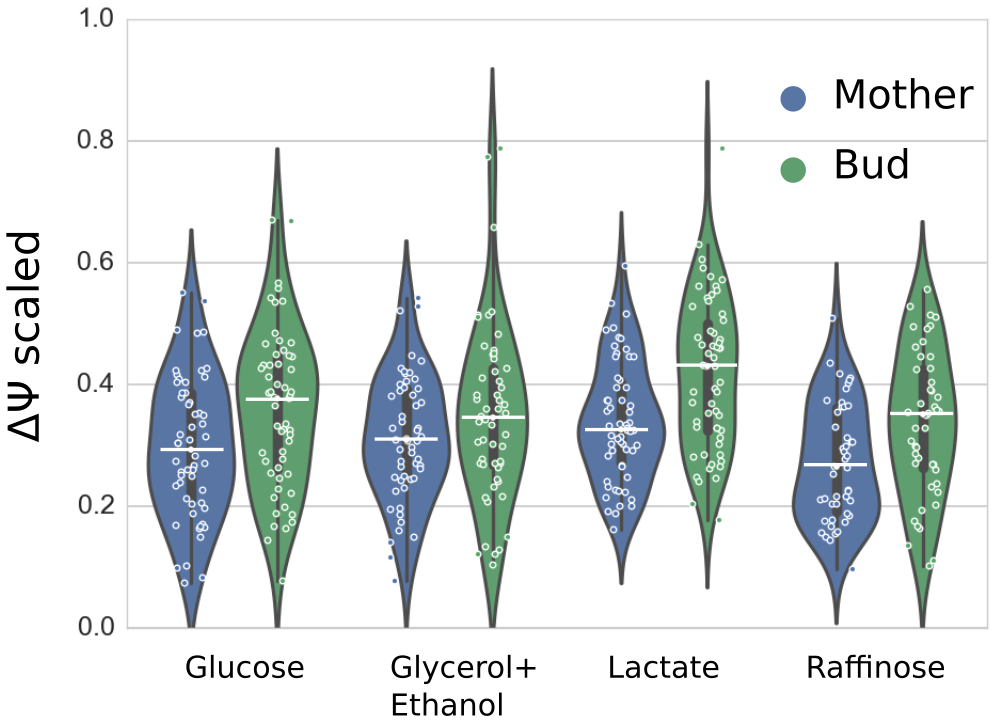
\includegraphics[width=.68\textwidth]{mbviol}
    \caption[Buds have higher mitochondrial membrane potential (ΔΨ) compared to their mothers]{Buds have higher mitochondrial membrane potential (ΔΨ) compared to their mothers.\\Shown in this figure is the distribution of the scaled ΔΨ distribution of all buds and mothers grown in different carbon sources. The scaled ΔΨ represents the mean ΔΨ value of a particular bud or mother scaled to the min and max ΔΨ value for that cell. Buds have a statistically significant higher ΔΨ compared to their mothers for all conditions ($p$<0.05 based on Wilcoxon signed rank test for paired samples, with post-hoc multiple testing correction).\\\emph{White bars indicate the median values for the scaled ΔΨ.\\Number of mother-bud pairs---Glucose=56, Glycerol+Ethanol=54, Lactate=58, Raffinose=46}}\label{fig:mbviol}
\end{figure}
%
%
\begin{figure}[htp]
	\centering
    \hspace*{1in}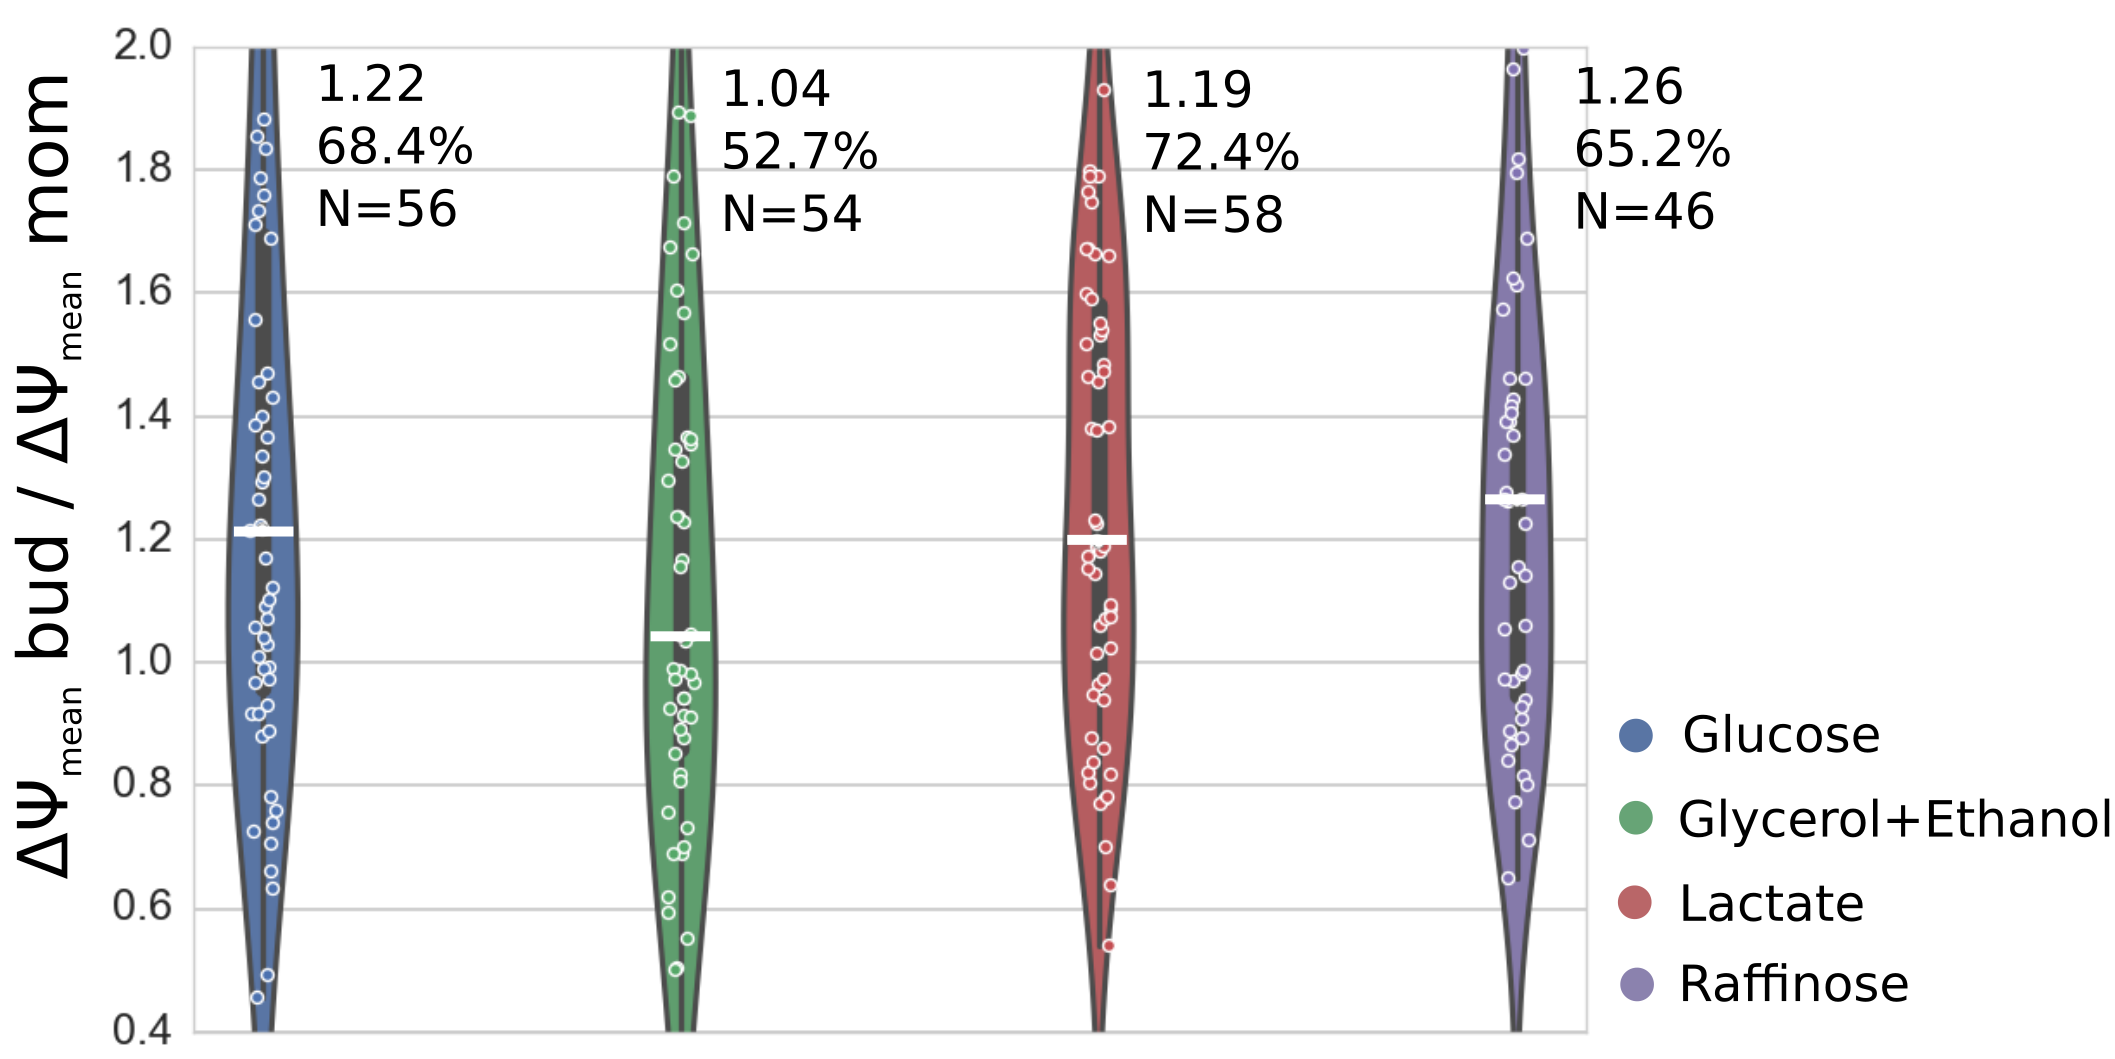
\includegraphics[width=.8\textwidth]{fraviol}
    \caption[Distribution of ΔΨ$_\mathrm{bud}/$ΔΨ$_\mathrm{mother}$ in different carbon sources]{Distribution of ΔΨ$_\mathrm{bud}/$ΔΨ$_\mathrm{mother}$ in different carbon sources.\\The ratio of ΔΨ$_\mathrm{bud}/$ΔΨ$_\mathrm{mother}$ was used to quantify the number of cells where the average ΔΨ of the bud was higher than the mother as well as the average magnitude of this ratio. The first row of numbers represent the average magnitude of ΔΨ$_\mathrm{bud}/$ΔΨ$_\mathrm{mother}$. The mean of this magnitude was about 1.2 (20\% higher ΔΨ in the bud). The second row of numbers represent the proportion of mother-bud pairs where the bud had a higher ΔΨ compared to the mother. The last row of numbers represent the number of mother-bud pairs for each population.\\\emph{White bars indicate the median values for the ratio of} ΔΨ$_\mathrm{bud}/$ΔΨ$_\mathrm{mother}$.}\label{fig:fraviol}
\end{figure}
%
\subsection{Mitochondria display different gradients of ΔΨ along the mother-bud axis}
To analyze the distribution of ΔΨ along the mother-bud cell axis, we partitioned cells into a mother and bud region and defined two separate coordinate systems (one for the mother and one for the bud, each scaled 0--1). The intersection point (bud neck) had a value of 1 for the mother and 0 for the bud in their respective coordinate systems. The corresponding plot for the mother regions for each carbon source is shown in \Fref{fig:aldymom}. For the bud regions, we further partitioned the plots according to bud volumes, as these represented different stages of bud growth. The partition bins are labeled as 'binvol' in \Fref{fig:aldybud}, representing bud volume in \si{\micron\cubed}). The ΔΨ values in these plots were scaled to the min and max of the entire cell axis (mother and bud) for each cell. We observe a pattern where ΔΨ was lowest at the mother distal end, gradually rises and plateaus halfway in the mother cell for the populations of glycerol+ethanol, lactate and raffinose (\Fref{fig:aldymom}). For glucose,  ΔΨ does not seem to plateau but appears to continue to rise, although the error bars are large enough that a plateau cannot be ruled out.
%
\begin{figure}[htp]
	\centering
    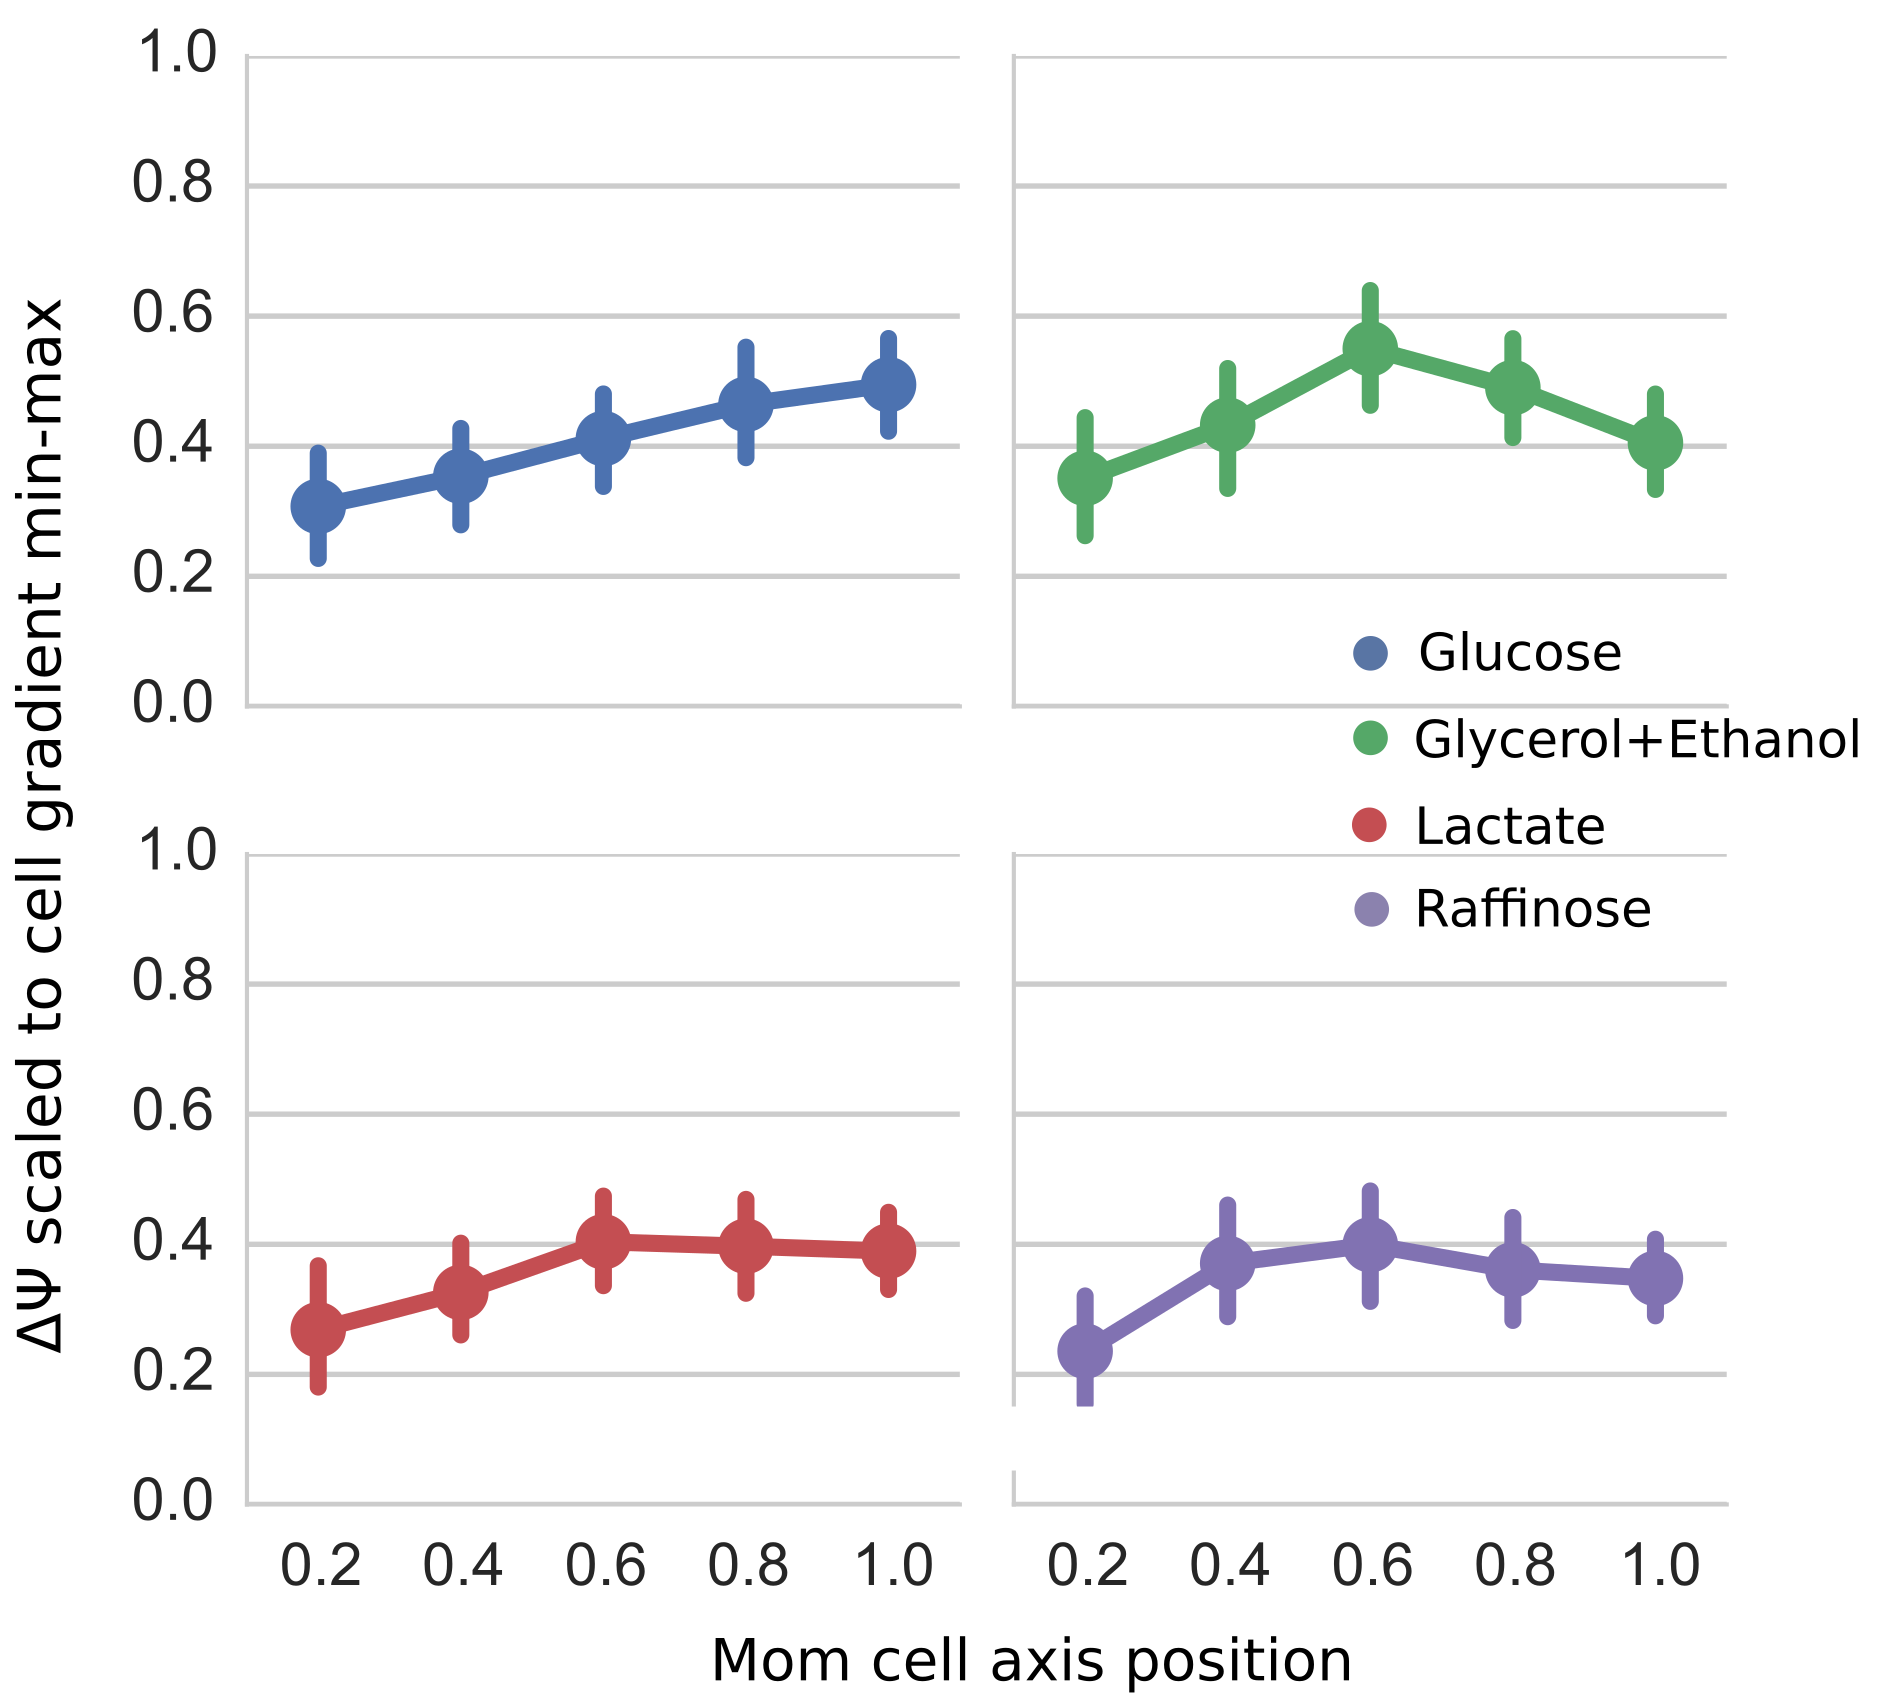
\includegraphics[width=.52\textwidth]{aldymom}
    \caption[Spatial distribution of ΔΨ along the mother cell axis]{Spatial distribution of ΔΨ along the mother cell axis.\\Shown in this figures is a plot of the average ΔΨ at each position along the mother axis (position 0 is at the mother distal end away from the bud neck, position 1 is at the bud neck). ΔΨ gradually increases from the mother distal end and plateaus halfway along the axis.\\\emph{Error bars represent the 95\% confidence interval of the median ΔΨ at each position along the mother cell axis.\\Number of cells---Glucose=56, Glycerol+Ethanol=54, Lactate=58, Raffinose=46}}\label{fig:aldymom}
\end{figure}
%

It was harder to discern a clear pattern for the progression of ΔΨ in buds (\Fref{fig:aldybud}). Due to partitioning the buds into different bud volumes, the sample numbers were reduced for each bud volume category and hence the error bars were larger compared to the mother plots. It appears that larger buds have a more consistent/flat ΔΨ distribution compared to smaller buds, except for the case of raffinose. Consistent with the results from \Fref{sec:frady}, the bud region displays a higher average ΔΨ compared to the mother regions. There appears to be a discontinuity (i.e. a sudden rise in ΔΨ) at the bud neck region when moving from the mother to the bud. 
%
\begin{figure}[htp]
	\centering
    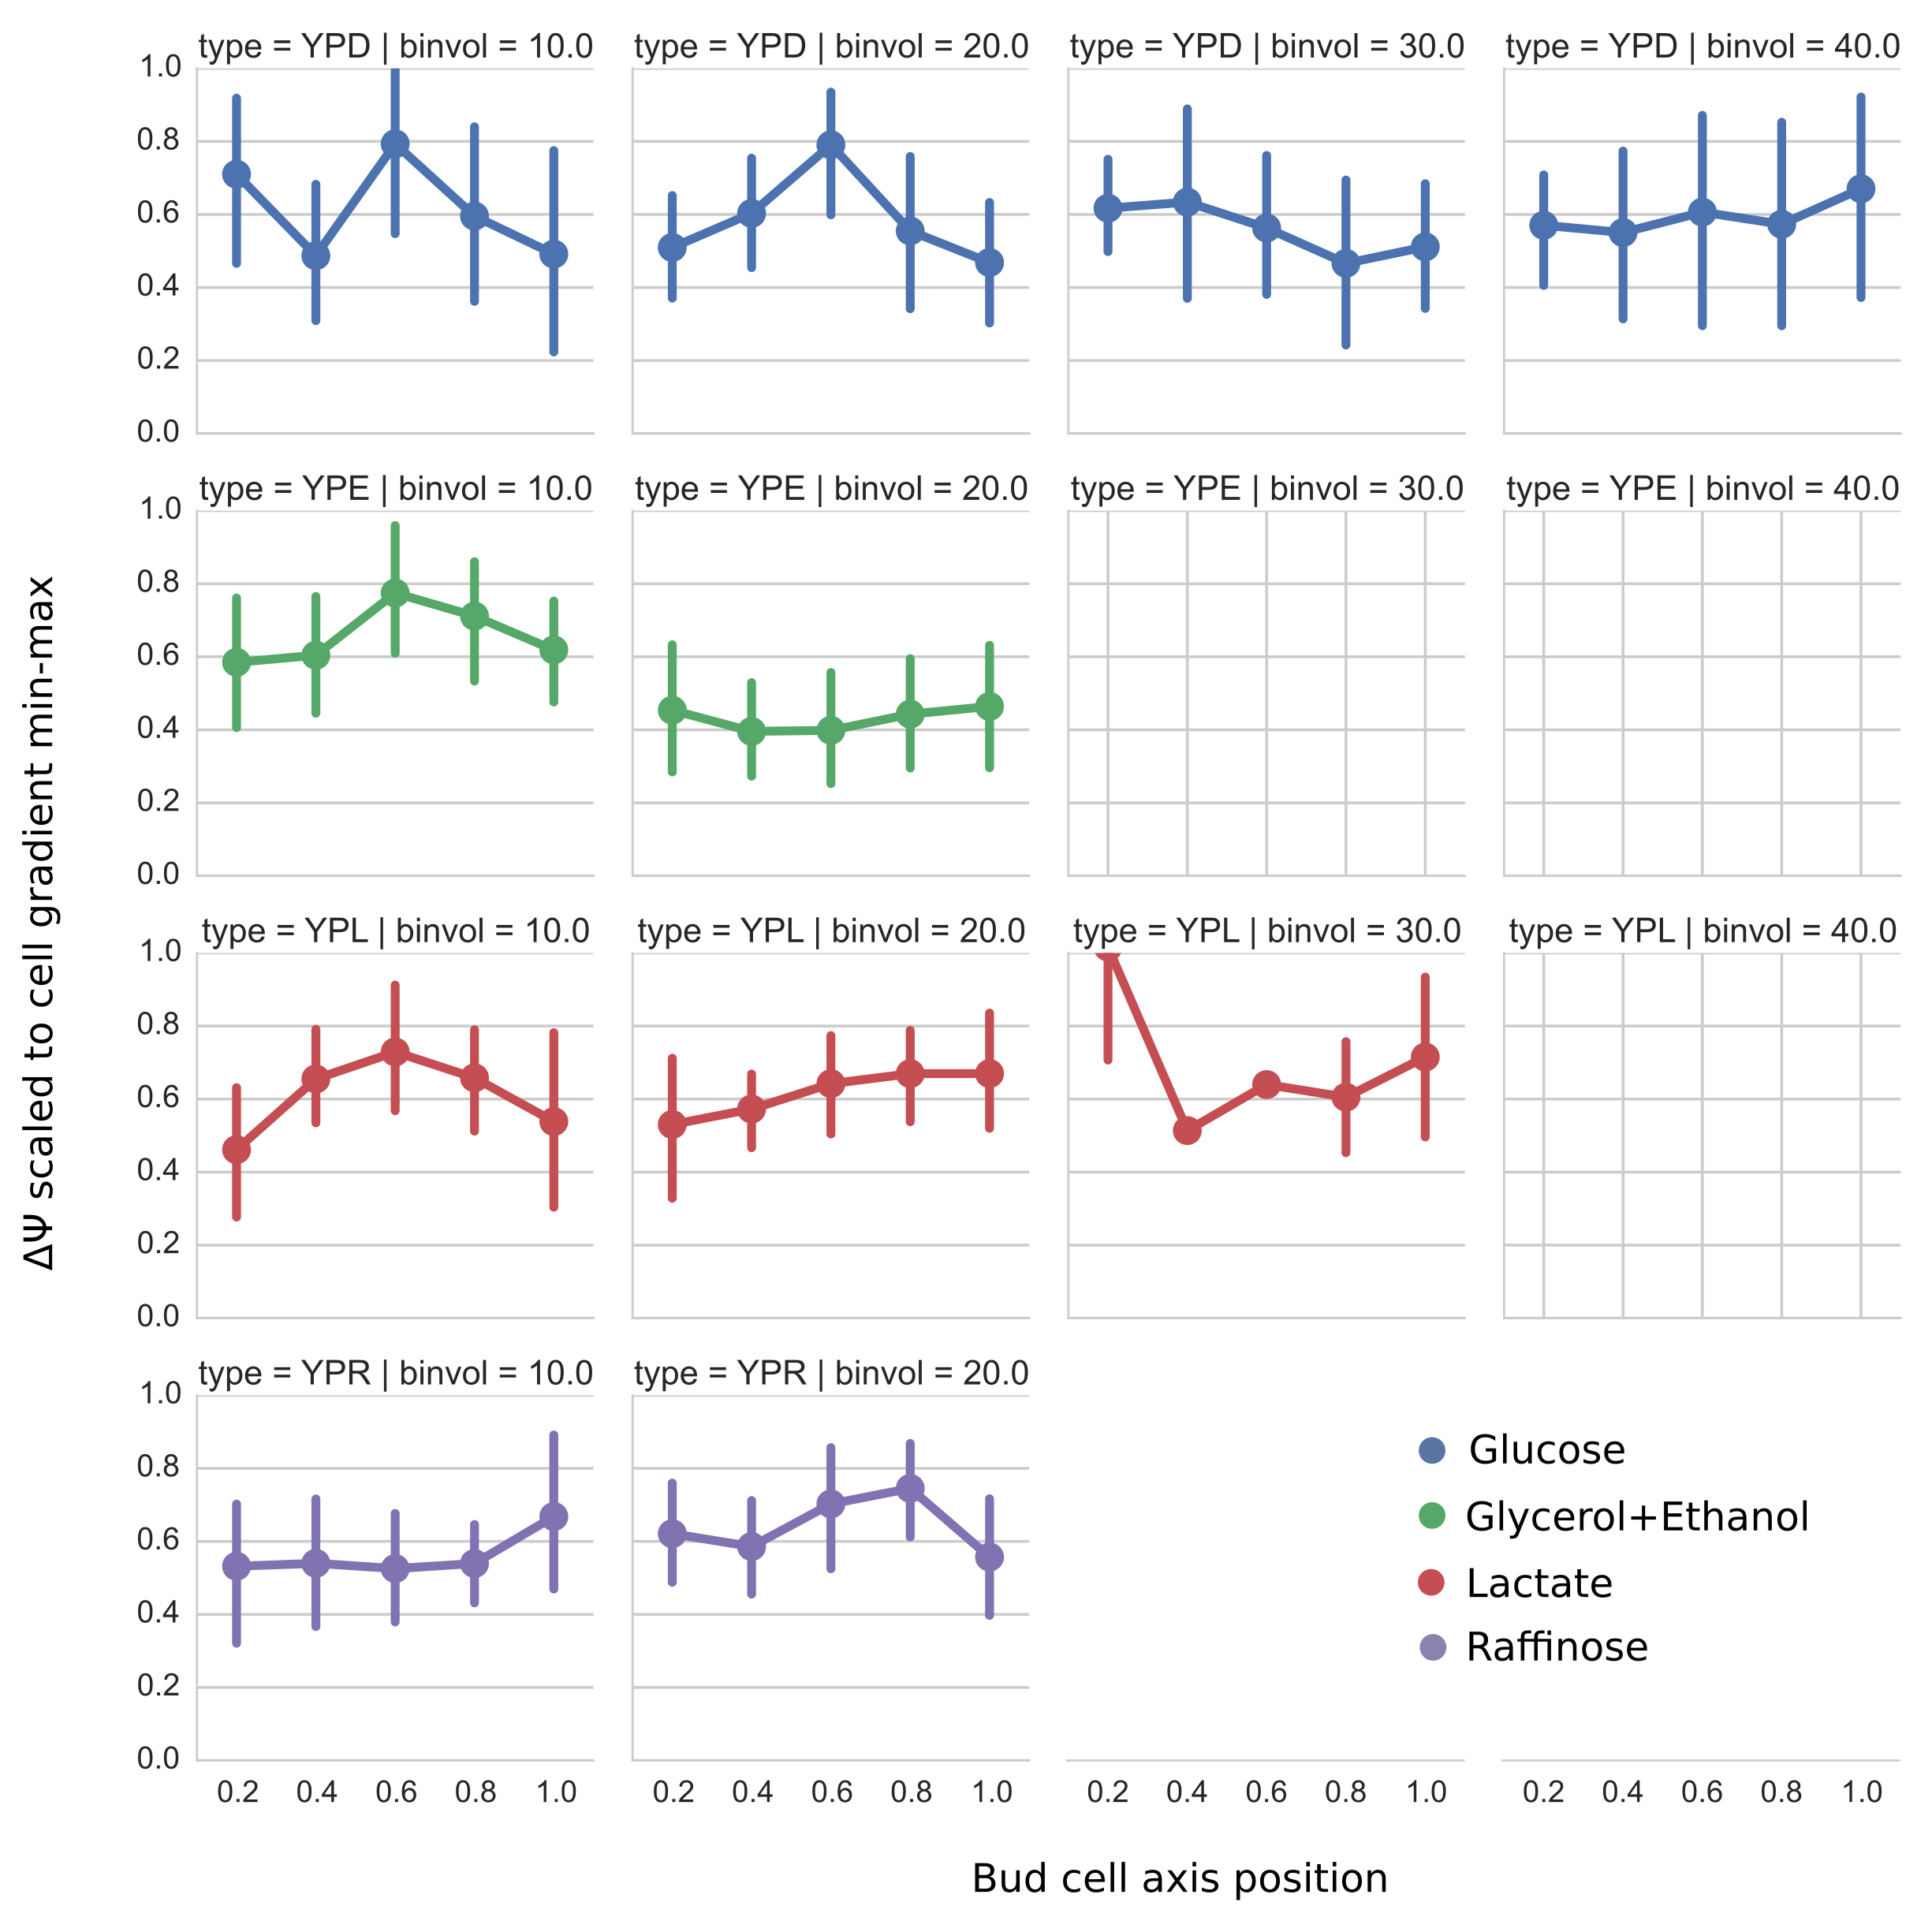
\includegraphics[width=.8\textwidth]{aldybud}
    \caption[Spatial distribution of ΔΨ along the bud cell axis]{Spatial distribution of ΔΨ along the bud cell axis.\\Shown in this figures is a plot of the average ΔΨ at each position along the bud axis (position 0 is at the the bud neck, position 1 is at bud end opposite the bud neck). The buds are partitioned according to their volume. The partitioning bins are labeled as 'binvol', representing bud volume in \si{\micron\cubed}). Larger buds display a more consistent/flat ΔΨ distribution compared to smaller buds, except for the case of raffinose.\\\emph{Error bars represent the 95\% confidence interval of the median ΔΨ at each position along the bud cell axis.\\Number of cells---Glucose=56, Glycerol+Ethanol=54, Lactate=58, Raffinose=46}}\label{fig:aldybud}
\end{figure}
%
\subsection{Mitochondrial ΔΨ asymmetry is maintained during the budding progression}
We tracked the ratio of bud ΔΨ to mother ΔΨ as a function of budding progression (defined in \Fref{sec:cellcycle}) to see if there was a change in the functional asymmetry of ΔΨ as budding progressed. As shown in \Fref{fig:frabud}, with the exception of glycerol+ethanol this ratio is maintained above 1 throughout budding progression. This indicates that mitochondrial bud quality is maintained at a higher level throughout the cell cycle. Glycerol+ethanol grown cells display a reduction in this ratio to values below 1 at intermediate values of bud volume. We found that while glycerol+ethanol had the lowest bud ΔΨ to mother ΔΨ ratio, for most of the budding progression it was above 1. We also partitioned the the data in \Fref{fig:frabud} according to bud volumes, similar to what was done for the bud ΔΨ gradient in \Fref{fig:aldybud}. As shown in \Fref{fig:frafacet}, there does not appear to be an obvious change in the ΔΨ asymmetry between cells with smaller and larger buds.
%
\begin{figure}[htp]
	\centering
    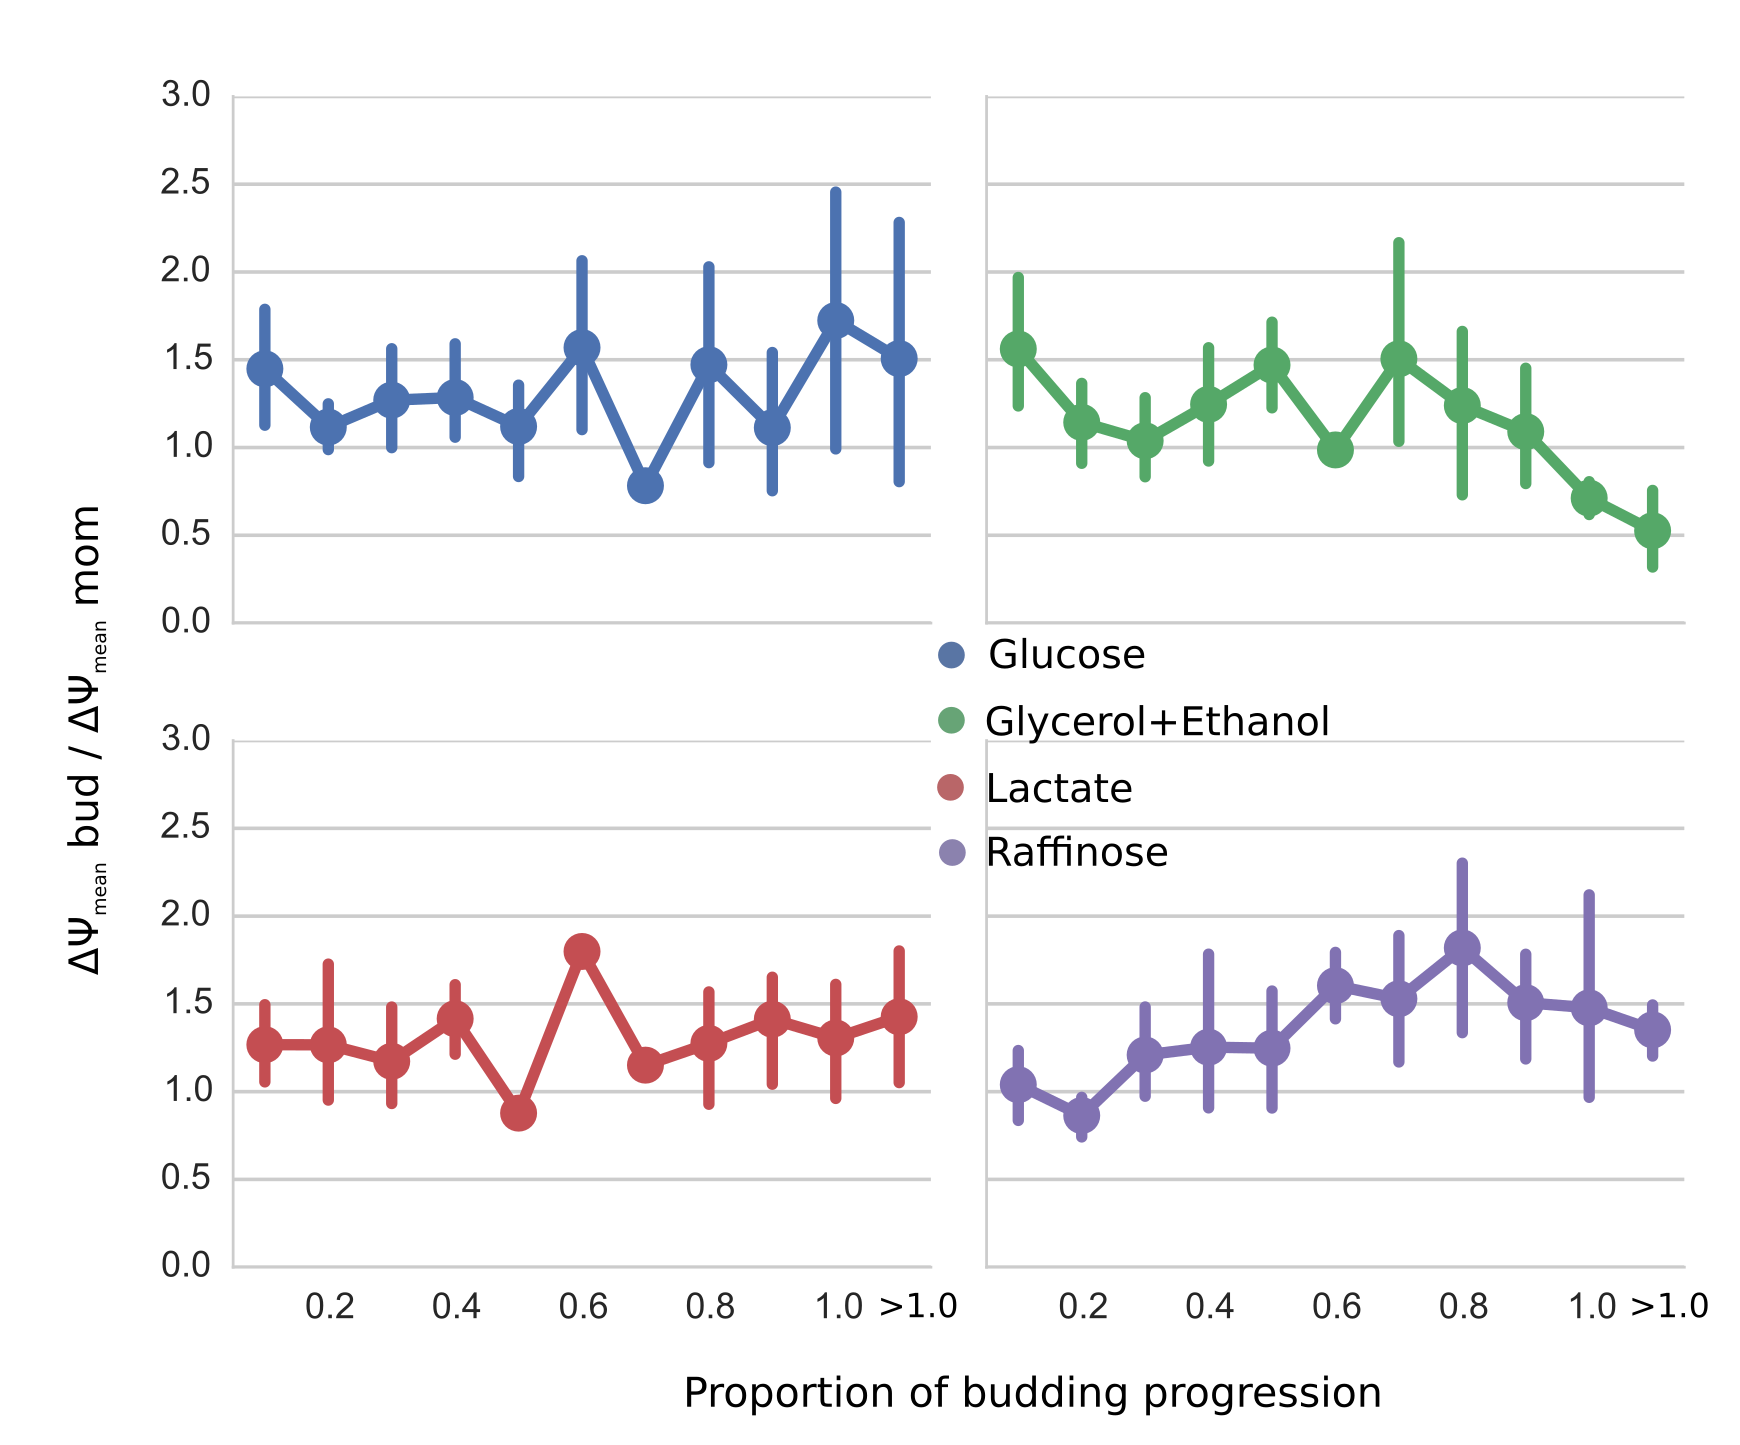
\includegraphics[width=.75\textwidth]{frabud}
    \caption[Mitochondrial ΔΨ asymmetry is maintained throughout the cell cycle]{Mitochondrial ΔΨ asymmetry is maintained throughout the cell cycle.\\The ΔΨ$_\mathrm{bud}/$ΔΨ$_\mathrm{mother}$ ratio for each cell was plotted as a function of budding progression. There was no significant difference in this ratio as we moved from early in the cell cycle to completion of cell division. This indicates that the mitochondrial ΔΨ asymmetry is maintained throughout the cell cycle.\\\emph{Error bars represent the 95\% confidence interval of the median ΔΨ$_\mathrm{bud}/$ΔΨ$_\mathrm{mother}$ ratio at each value for budding progression.\\Number of cells---Glucose=56, Glycerol+Ethanol=54, Lactate=58, Raffinose=46}}\label{fig:frabud}
\end{figure}
%
%
\begin{figure}[htp]
	\centering
    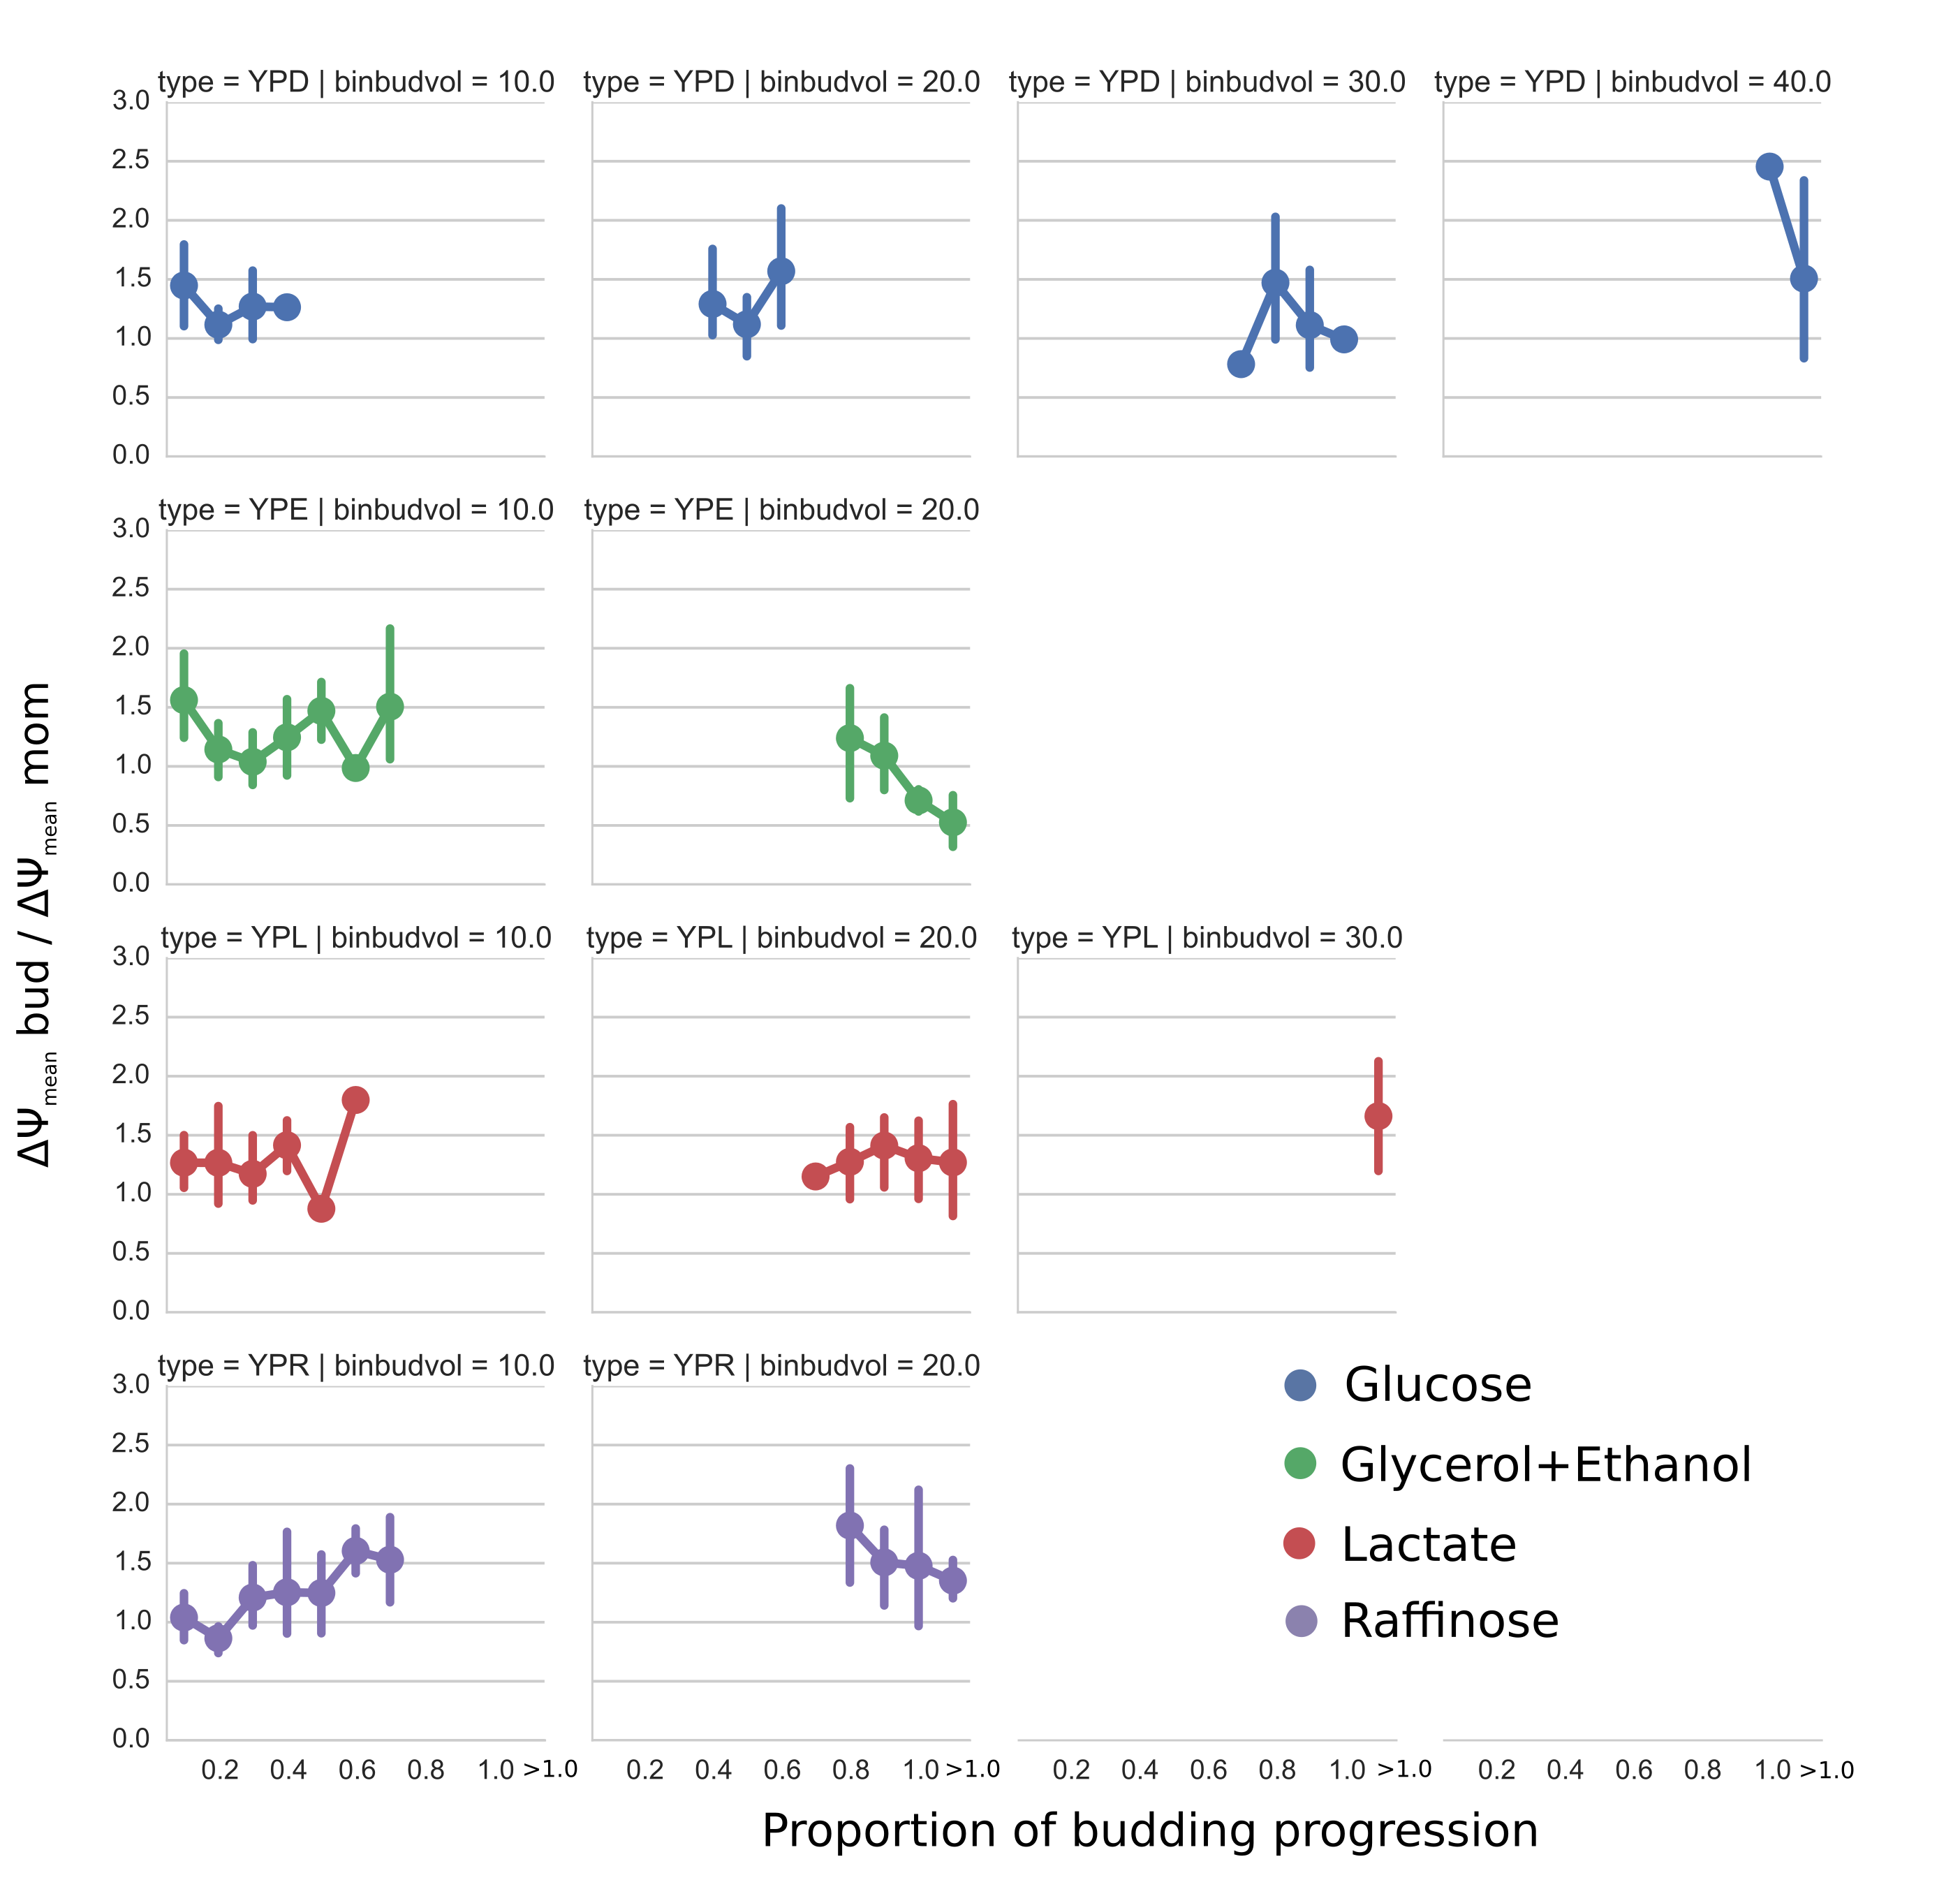
\includegraphics[width=.8\textwidth]{frafacet}
    \caption[Bud size has no effect on mitochondrial ΔΨ asymmetry in the cell]{Bud size has no effect on mitochondrial ΔΨ asymmetry in the cell.\\ ΔΨ$_\mathrm{bud}/$ΔΨ$_\mathrm{mother}$ ratio as a function of budding progression was plotted at different partitions of bud volumes. The partitioning bins are labeled as 'binvol', representing bud volume in \si{\micron\cubed}). There was no significant difference in ΔΨ asymmetry between cells with smaller and larger buds.}\label{fig:frafacet}
\end{figure}
%
\section{Discussion}
We have analyzed and confirmed that mitochondrial networks in yeast display an asymmetry of mitochondrial quality between mother and daughter cells (buds), similar to previously reported results. Our results were obtained after careful segmentation of the mother-bud axis in three dimensions as detailed in this chapter. We found that this asymmetry exists regardless of whether the cell was undergoing fermentation or aerobic respiration. This suggests that yeast preserve the machinery to preferentially distribute higher quality mitochondria to their buds even when respiration demand of the cell is low. This suggests that the distribution of mitochondria with higher levels of ΔΨ to the progeny (bud) is inherently essential not just for aerobic respiration but perhaps for other functions that are ΔΨ dependent, such as mitochondrial fusion and mitochondrial protein import \cite{dudek_mitochondrial_2013}. Our results also suggest that ΔΨ asymmetry persists throughout the entire budding progression cycle. This suggest that ΔΨ asymmetry results from a segregation mechanism that is active throughout the cell division cycle.
 
Our results showing a gradient of ΔΨ in the mother cell that plateaus halfway towards the bud is interesting as it suggests a possible mitochondrial quality segregation process occuring at the distal end of the mother cell. We speculate that the mechanism for this segregation process involves some sort of preferential retention of lower quality mitochondria at the distal end of the mother cell. Mitochondria are tethered at the mother end by a mitochondrial-ER-cortex-anchor (MECA) complex \cite{lackner2013endoplasmic}). This complex is absent from small buds and is localized to larger buds and mother cells. At least two proteins, Num1 and Mdm36 are essential components of this tethering complex. Thus one way to test our hypothesis on segregation of mitochondria at the mother distal end is to disrupt the expression of NUM1 or MDM36 to see if the ΔΨ gradient in the mother is altered or even abolished.

Our result showing a discontinuity and sudden increase in ΔΨ at the bud neck suggest another 'hurdle' or quality threshold that mitochondria must overcome to enter the bud. Another possibility is that the anchorage machinery at the bud tip preferentially binds to higher quality mitochondria. The Myo2 myosin has been implicated in transporting mitochondria across the bud neck \cite{fortsch2011myosin}. In addition, Mmr1 and Ypt11 are proteins that have been identified as having a role in binding mitochondria to Myo2. Recent studies indicate that mitochondria are tethered to the bud tip via interactions with the cortical ER (cER). Anchorage of mitochondria to cER has been shown to be dependent on Mmr1 \cite{swayne_role_2011}. Thus one way to investigate the mechanism of mitochondrial quality selection at the bud is to disrupt or modulate the expression of MYO2, MMR1 and YPT11 with a β-estradiol gene induction and protein degradation system \cite{mcisaac2011fast}. While there have been studies of functional asymmetry in mmr1Δ (for example in \cite{mcfaline-figueroa_mitochondrial_2011}), these have only focused on the differences in magnitude of ΔΨ asymmetry between mother and bud. Our method allows us to study how the spatial distribution of asymmetry and the discontinuity of ΔΨ at the bud neck is affected by deletion or modulation of MYO2, MMR1 and YPT11. Such an analysis provides a possible mechanistic insight into how the mitochondrial inheritance machinery plays a role in mitochondrial quality selection during cell division.

Interestingly we found that the magnitude of ΔΨ asymmetry between mother and bud was smallest in the glycerol+ethanol cells (\Fref{fig:fraviol}). We showed in \Fref{ch:three} that cells grown in glycerol+ethanol had the highest average ΔΨ. Perhaps this indicates that that there is a limit to the ΔΨ level that buds can inherit. Since glycerol+ethanol population has the highest overall ΔΨ compared to the other populations, a bud inheriting mitochondria with similar ΔΨ asymmetry levels as the other populations would have excessively high ΔΨ.

In conclusion, we have shown that the distribution of ΔΨ along the mother-bud axis displays some interesting features which put quantitative restrictions on any future mathematical models of how mitochondrial functional asymmetry is achieved. Our findings also suggests that the mitochondrial quality selection process involves the mitochondrial transport and tethering machinery. 

\chapter{Significance and future direction}\label{ch:seven}
\section{Significance}
We have developed a quantitative, multiscale data analysis framework that is able to provide an integrated overview of the relationship between mitochondrial network structure and its bioenergetic state. We showed that by applying our framework onto populations of cells with different respiration states, we were able to provide insight into the changes in their mitochondrial ultrastructure, network structure and functional asymmetry during cell division.

Our first contribution to the field is providing the basic tools and formalizing an approach to perform structure-function relationship of yeast mitochondrial networks in an integrated, quantitative manner. The data that we obtained could offer another contribution by providing the parameters and constraining the solution space for a computational model of mitochondrial quality control through fission and fusion events. The present computational models of how mitochondrial dynamics regulate mitochondrial quality do not integrate detailed spatial and topological information of the network and how function is related to these spatial features \cite{mouli_frequency_2009,patel_optimal_2013}. This is provided for in our dataset at multiple size scales. The weakness in our dataset is a lack of sufficient temporal resolution such that we were unable to incorporate fission and fusion rates into our pipeline.
 
Here we discuss several directions for future research that we believe can extend the utility of the tools developed and provide further insight into the biology of the mitochondrial network.
\section{Improved spatial resolution}
The spinning disk confocal microscope platform that we use provides the best balance between spatial and temporal resolution with minimal phototoxicity. It allows us to obtain a multiscale understanding of structure and function relationship in yeast mitochondrial networks. However if we are only interested in for example, the ultrastructure level we could use different imaging methods such as superresolution microscopy, deconvolution or electron microscopy.

While MitoGraph v2.0 is currently very consistent (96.7\% reproducibility \cite{viana_chapter_2015}), its accuracy tends to suffer especially in regions where the mitochondrial network is very dense. These dense regions are precisely the regions of most interest to our network connectivity analysis, as they have much more entropy (information content) in their topology. Superresolution and deconvolution microscopy could potentially resolve these difficult regions for MitoGraph to work well. The main barriers to superresolution, apart from cost and access, is the tradeoff between spatial and temporal resolution. Superresolution techniques tend to be very slow as they must sample the image many times to obtain sub-pixel localization (STORM \cite{rust_sub-diffraction-limit_2006} and PALM \cite{betzig_imaging_2006}) or multiplex multiple frequency bands (structured illumination \cite{kner_super-resolution_2009}). However this problem might be overcome if imaging rates are improved substantially \cite{abrahamsson_fast_2013,babcock_fast_2013} along with the use of improved bright fluorescent proteins that have sufficiently high signal so that faster acquisition speeds can be used. Deconvolution of the images obtained from the spinning disk could potentially increase the resolution as well, however it would require a careful calibration of the point spread function of the system and subsequent validation of the deconvolved images before we can be confident in the data analysis.

In fact superresolution would be useful not just in increasing the accuracy of the skeletonization by MitoGraph v2.0, but would also allow direct observations of the cristae structure that we probed indirectly in \Fref{ch:four}. Preliminary images have already shown that live cell imaging of cristae stained with a mitochondrial membrane dye (Mitotracker) is possible (\url{http://www.nikon.com/products/instruments/lineup/bioscience/s-resolution/nsim/}), however at present this system requires a sampling level that results in phototoxicity to the mitochondria.

Another way to obtain improved spatial resolution is to used electron microscopy (EM) to directly image the ultrastructure. In \Fref{ch:four} we mentioned that line scan analysis of the data from several studies using EM have confirmed that tubule thickness increases when mitochondria are undergoing respiration. However, with the exception of very old studies from the 60's, these EM imaging studies were not directly focused on changes to mitochondrial cross sectional width and the distribution of tubule thickness under different respiratory conditions. Hence it could be an interesting research topic to use EM to study changes to the morphology and size of the mitochondrial ultrastructure in yeast when their respiratory state is perturbed using different carbon sources. However this kind of study suffers from low throughput and requires a steep learning curve, therefore a collaboration with a group that specializes in EM or even EM tomography would be ideal.
\section{Genetically encoded functional sensors}
The mapping of function onto mitochondrial networks can be greatly improved with a fluorescent protein marker for mitochondrial membrane potential (ΔΨ). The expression of a fluorescent protein marker for ΔΨ would in theory have much less variability (especially if it was integrated into the genome) compared to cell to cell uptake variability of a dye. This would allow an absolute value of ΔΨ to be used based on the Nernst equation, thus enabling one to make direct comparisons of ΔΨ between cells growing in the same carbon source. However at present the current generation of fluorescent proteins that are voltage sensitive suffer from two huge barriers \cite{akemann_imaging_2010,kralj_optical_2012,sunita_ghimire_gautam_exploration_2009}---they are very difficult to target and be expressed correctly on the inner mitochondrial membrane, and perhaps even more important their fluorescent signal is so low and requires so much laser excitation power that the mitochondrial network is degraded beyond the point of observation due to photodamage.

However, it is worth mentioning that our pipeline can be adapted to any functional sensor that can be targeted specifically to mitochondrial function. For example we could use a genetically encoded redox sensor (roGFP), a hydrogen peroxide sensor (HyPer) or superoxide sensor (mt-cpYFP), an ATP sensor (Ateam) or ADP/ATP ratio sensor (Perceval) and so on (references and reviews in \cite{newman_genetically_2011}). The challenge of these sensors are again the same as in the membrane voltage sensor, namely signal to noise ratio and correct localization to the mitochondria. However with so many options it is likely that at least one of them can be successfully adapted to serve as a genetically encoded marker for mitochondrial functional state.
\section{Refinement in experimental setup}
In \Fref{ch:three} we mentioned that we only measured basal respiration rates due to the difficulty of using a Clark electrode to measure oxygen consumption rates in live yeast cells. The use of a Seahorse XF analyzer would enable us to determine the respiratory control ratios and spare respiratory capacity of mitochondria from cells in different carbon sources. This would then confirm or disprove our theory that mitochondria in lactate and raffinose are respiring less efficiently that in glycerol+ethanol.

The results from \Fref{ch:five} indicate that there is no relationship between mitochondrial function (ΔΨ) and connectivity within specific regions of the mitochondrial network. However one of our assumptions was that highly connected regions were also the sites of higher mitochondrial fusion and fission activity. While our results indicate that this is not true at the global level, it might still be true within localized areas of the network. This would require dynamic data (i.e. time courses where we can observe sites of fission and fusion) to distinguish areas of the network with high fusion activity. Only with this data can we conclusively say whether there is a correlation between the rate of mitochondrial dynamics and function/ ΔΨ. The difficulty in obtaining dynamic data is that it is very difficult to segment automatically mitochondrial fission and fusion sites, although work is ongoing to enable this functionality in MitoGraph. We also observed no functional dependence of mitophagy with ΔΨ in isolated mitochondrial fragments, but without following isolated fragments of mitochondria in real time and determining which ones are targeted for autophagy, we cannot conclusively say that mitophagy has no functional selection criteria. Furthermore we would also need to label the vacuoles or some other part of the autophagic machinery in order to have a reliable marker for mitophagy events.
 
In  \Fref{ch:six} we present some interesting findings regarding the distribution of ΔΨ along the mother daughter axis. Our preliminary results indicate that ΔΨ increases and then plateaus halfway along the mother cell axis. In addition buds maintain a higher level of ΔΨ throughout the entire cycle. Our data provides some constraints on any future mathematical models of how mitochondrial functional asymmetry is achieved. Our findings also suggests that the mitochondrial quality selection process involves the mitochondrial transport and tethering machinery. By applying our pipeline on deletion mutants for transport and tethering proteins, we could potentially gain some mechanistic insight into the relationship between the mitochondrial inheritance machinery and quality selection during cell division.





























% These commands fix an odd problem in which the bibliography line
% of the Table of Contents shows the wrong page number.
\clearpage
\phantomsection

% "References should be formatted in style most common in discipline",
% abbrv is only a suggestion.
\bibliographystyle{ieeetr}
\bibliography{zotero}

% The Thesis Manual says not to include appendix figures and tables in
% the List of Figures and Tables, respectively, so these commands from
% the caption package turn it off from this point onwards. If needed,
% it can be re-enabled later (using list=yes argument).
\captionsetup[figure]{list=no}
\captionsetup[table]{list=no}

% If you have an appendix, it should come after the references.
% The original template (from Trevor) had a custom \appendix command,
% but I found it to break figure/table counters. I'm not sure how
% reliable my fix is, so I ended up reverting back to the standard
% latex version, and renaming the custom command to \myappendix.  You
% can try both and see how things work out:
% 1) Call \appendix once, and then make each appendix a \chapter
% 2) Call \myappendix once, and then make each appendix a \section.

\appendix
\chapter{Supplementary figures}
\begin{figure}[htp]
		\centering
	    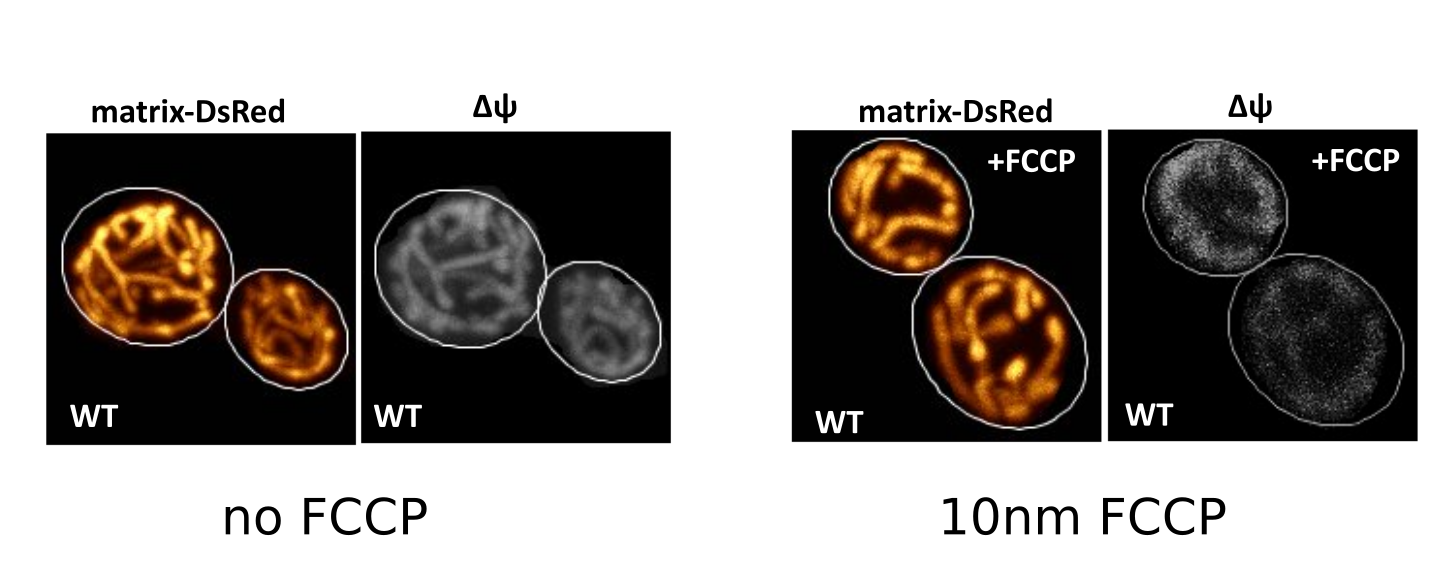
\includegraphics[width=\textwidth]{fccp}
	    \caption{Shown in this figure are images of cells stained with 100nm of DiOC$_6$, a membrane potential dependent dye (ΔΨ). The image on the left is a cell that is undergoing respiration and has normal levels of ΔΨ. The image on the right is a cell that has been treated with an uncoupler of ΔΨ, FCCP. The ΔΨ of the mitochondria is almost completely abolished after treatment, indicating that the dye was not suffering from auto-quenching (i.e. DiOC$_6$ signal intensity was proportional to ΔΨ).\\[2ex]\emph{Image provided courtesy of V.Jayashankar.}}\label{fig:fccp}
\end{figure}
%
%
\begin{figure}[htp]
		\centering
	    \includegraphics[width=\textwidth]{grwthcvs}
	    \caption{Shown in this figure are the growth curves for 2 replicates of yeast undergoing exponential growth in either YP+2\% glycerol+2\% ethanol or YP+2\% lactate. The doubling times for lactate was just slightly longer than glycerol+ethanol (3.2 hours vs 2.9 hours).}\label{fig:grwtcvs}
\end{figure}
%
%
\begin{figure}[htp]
		\centering
	    \includegraphics[width=\textwidth]{meli}
	    \caption{Shown in this figure are streak plates of W303a strain used in this thesis together with a s288c strain to check for growth viability on melibiose and raffinose. The plates were yeast extract+peptone+either 2\% melibiose or 2\% raffinose. Imaging of the plates was taken 4 days after streaking.}\label{fig:meli}
\end{figure}
%
%	    
\chapter{Statistical tables}
%
{
\sisetup{
round-mode = places,
round-precision = 4}
\begin{table}
\caption{Tables of statistical tests using rank-sums test with Holms -Sidak post-hoc multiple testing correction.\\Labels---YPD = glucose, YPE = glycerol+ethanol, YPL = lactate, YPR = raffinose\\stat = rank sum statistic\\p-val = uncorrected rank sum $p$ value\\
pval-corr. = Holms-Sidak multiple testing correction $p$ value\\
Test criteria--- reject null hypothesis that there is no difference between the medians of the group if pval-corr < 0.05\\Values with 0.0000 indicate $p$ < 1×10$^{-27}$}\label{tab:tests}
\centering
\footnotesize
\begin{tabular}{x{2cm}x{2cm}S[round-mode = places,round-precision = 0,table-format=4.0]S[table-format=2.4]S[table-format=2.4]c}
\toprule
\multicolumn{2}{c}{\textbf{Cell mito avg. ΔΨ scl.}}&&&\\
\cmidrule{1-2}
\textbf{group1} & \textbf{group2} & \textbf{stat} &\textbf{p-val}&\textbf{p-val corr.}& \textbf{reject}  \\
\midrule
      YPD       &       YPE       &     5052.0    &     0.2607    &       0.5661       &      False       \\
      YPD       &       YPL       &     4605.0    &     0.0120     &       0.0619       &      False       \\
      YPD       &       YPR       &     4579.0    &     0.4705    &       0.5661       &      False       \\
      YPE       &       YPL       &     5592.0    &     0.0352    &       0.1334       &      False       \\
      YPE       &       YPR       &     5028.0    &     0.2429    &       0.5661       &      False       \\
      YPL       &       YPR       &     4584.0    &     0.0106    &       0.0619       &      False       \\
\bottomrule
\end{tabular}
\end{table}
%
\begin{table}
\centering
\footnotesize
\begin{tabular}{x{2cm}x{2cm}S[round-mode = places,round-precision = 0,table-format=4.0]S[table-format=2.4]S[table-format=2.4]c}
\toprule
\multicolumn{2}{c}{\textbf{Cell mito avg. ΔΨ raw}}&&&\\
\cmidrule{1-2}
\textbf{group1} & \textbf{group2} & \textbf{stat} &\textbf{p-val}&\textbf{p-val corr.}& \textbf{reject}  \\
\midrule
      YPD       &       YPE       &     629.0     &      0.0      &        0.0         &       True       \\
      YPD       &       YPL       &     1402.0    &      0.0      &        0.0         &       True       \\
      YPD       &       YPR       &     939.0     &      0.0      &        0.0         &       True       \\
      YPE       &       YPL       &     4198.0    &      0.0      &        0.0         &       True       \\
      YPE       &       YPR       &     4085.0    &     0.0019    &       0.0038       &       True       \\
      YPL       &       YPR       &     4985.0    &     0.0795    &       0.0795       &      False       \\
\bottomrule
\end{tabular}
\end{table}
%
\begin{table}
\centering
\footnotesize
\begin{tabular}{x{2cm}x{2cm}S[round-mode = places,round-precision = 0,table-format=4.0]S[table-format=2.4]S[table-format=2.4]c}
\toprule
\multicolumn{2}{c}{\textbf{Cell mito std. ΔΨ scl.}}&&&\\
\cmidrule{1-2}
\textbf{group1} & \textbf{group2} & \textbf{stat} &\textbf{p-val}&\textbf{p-val corr.}& \textbf{reject}  \\
\midrule
      YPD       &       YPE       &     5050.0    &     0.2592    &       0.6337       &      False       \\
      YPD       &       YPL       &     5273.0    &     0.2221    &       0.6337       &      False       \\
      YPD       &       YPR       &     4368.0    &     0.2669    &       0.6337       &      False       \\
      YPE       &       YPL       &     5697.0    &     0.0549    &       0.2874       &      False       \\
      YPE       &       YPR       &     4728.0    &     0.0815    &       0.3463       &      False       \\
      YPL       &       YPR       &     5606.0    &     0.4915    &       0.6337       &      False       \\
\bottomrule
\end{tabular}
\end{table}

%
\begin{table}
\centering
\footnotesize
\begin{tabular}{x{2cm}x{2cm}S[round-mode = places,round-precision = 0,table-format=4.0]S[table-format=2.4]S[table-format=2.4]c}
\toprule
\multicolumn{2}{c}{\textbf{Cell mito std. ΔΨ raw}}&&&\\
\cmidrule{1-2}
\textbf{group1} & \textbf{group2} & \textbf{stat} &\textbf{p-val}&\textbf{p-val corr.}& \textbf{reject}  \\
\midrule
      YPD       &       YPE       &     1060.0    &      0.0      &        0.0         &       True       \\
      YPD       &       YPL       &     2201.0    &      0.0      &        0.0         &       True       \\
      YPD       &       YPR       &     1398.0    &      0.0      &        0.0         &       True       \\
      YPE       &       YPL       &     4205.0    &      0.0      &        0.0         &       True       \\
      YPE       &       YPR       &     4219.0    &     0.005     &       0.0099       &       True       \\
      YPL       &       YPR       &     4860.0    &     0.0457    &       0.0457       &       True       \\
\bottomrule
\end{tabular}
\end{table}
%
\begin{table}
\centering
\footnotesize
\begin{tabular}{x{2cm}x{2cm}S[round-mode = places,round-precision = 0,table-format=4.0]S[table-format=2.4]S[table-format=2.4]c}
\toprule
\multicolumn{2}{c}{\textbf{Network avg. deg.}}&&&\\
\cmidrule{1-2}
\textbf{group1} & \textbf{group2} & \textbf{stat} &\textbf{p-val}&\textbf{p-val corr.}& \textbf{reject}  \\
\midrule
      YPD       &       YPE       &     3685.0    &     0.0001    &       0.0003       &       True       \\
      YPD       &       YPL       &     3331.0    &      0.0000      &        0.0         &       True       \\
      YPD       &       YPR       &     3279.5    &     0.0003    &       0.0011       &       True       \\
      YPE       &       YPL       &     5791.5    &     0.0794    &       0.2198     &      False       \\
      YPE       &       YPR       &     5280.5    &     0.4564    &       0.4564       &      False       \\
      YPL       &       YPR       &     4999.0    &     0.0842    &       0.2198       &      False       \\
\bottomrule
\end{tabular}
\end{table}
%
\begin{table}
\centering
\footnotesize
\begin{tabular}{x{2cm}x{2cm}S[round-mode = places,round-precision = 0,table-format=4.0]S[table-format=2.4]S[table-format=2.4]c}
\toprule
\multicolumn{2}{c}{\textbf{Shortest path len.}}&&&\\
\cmidrule{1-2}
\textbf{group1} & \textbf{group2} & \textbf{stat} &\textbf{p-val}&\textbf{p-val corr.}& \textbf{reject}  \\
\midrule
      YPD       &       YPE       &     3292.0    &      0.0      &        0.0         &       True       \\
      YPD       &       YPL       &     808.5     &      0.0      &        0.0         &       True       \\
      YPD       &       YPR       &     2716.0    &      0.0      &        0.0         &       True       \\
      YPE       &       YPL       &     2256.0    &      0.0      &        0.0         &       True       \\
      YPE       &       YPR       &     5138.0    &     0.3296    &       0.3296       &      False       \\
      YPL       &       YPR       &     2140.5    &      0.0      &        0.0         &       True       \\
\bottomrule
\end{tabular}
\end{table}
%
\begin{table}
\centering
\footnotesize
\begin{tabular}{x{2cm}x{2cm}S[round-mode = places,round-precision = 0,table-format=4.0]S[table-format=2.4]S[table-format=2.4]c}
\toprule
\multicolumn{2}{c}{\textbf{Number of edges}}&&&\\
\cmidrule{1-2}
\textbf{group1} & \textbf{group2} & \textbf{stat} &\textbf{p-val}&\textbf{p-val corr.}& \textbf{reject}  \\
\midrule
      YPD       &       YPE       &     2996.0    &      0.0      &        0.0         &       True       \\
      YPD       &       YPL       &     524.0     &      0.0      &        0.0         &       True       \\
      YPD       &       YPR       &     2804.5    &      0.0      &        0.0         &       True       \\
      YPE       &       YPL       &     1933.0    &      0.0      &        0.0         &       True       \\
      YPE       &       YPR       &     5142.0    &     0.3329    &       0.3329       &      False       \\
      YPL       &       YPR       &     1461.0    &      0.0      &        0.0         &       True       \\
\bottomrule
\end{tabular}
\end{table}
%
\begin{table}
\centering
\footnotesize
\begin{tabular}{x{2cm}x{2cm}S[round-mode = places,round-precision = 0,table-format=4.0]S[table-format=2.4]S[table-format=2.4]c}
\toprule
\multicolumn{2}{c}{\textbf{Cell $\text{β}_{\V{geometric}}$}}&&&\\
\cmidrule{1-2}
\textbf{group1} & \textbf{group2} & \textbf{stat} &\textbf{p-val}&\textbf{p-val corr.}& \textbf{reject}  \\
\midrule
      YPD       &       YPE       &     3882.5    &     0.0004    &       0.0015       &       True       \\
      YPD       &       YPL       &     3695.5    &      0.0      &       0.0001       &       True       \\
      YPD       &       YPR       &     3121.0    &     0.0001    &       0.0003       &       True       \\
      YPE       &       YPL       &     6186.5    &     0.269     &       0.5672       &      False       \\
      YPE       &       YPR       &     5029.0    &     0.2436    &       0.5672       &      False       \\
      YPL       &       YPR       &     5585.5    &     0.4733    &       0.5672       &      False       \\
\bottomrule
\end{tabular}
\end{table}
%
\begin{table}
\centering
\footnotesize
\begin{tabular}{x{2cm}x{2cm}S[round-mode = places,round-precision = 0,table-format=4.0]S[table-format=2.4]S[table-format=2.4]c}
\toprule
\multicolumn{2}{c}{\textbf{Cell $\text{β}_{\V{topological}}$}}&&&\\
\cmidrule{1-2}
\textbf{group1} & \textbf{group2} & \textbf{stat} &\textbf{p-val}&\textbf{p-val corr.}& \textbf{reject}  \\
\midrule
      YPD       &       YPE       &     3982.0    &     0.0009    &       0.0034       &       True       \\
      YPD       &       YPL       &     3793.0    &      0.0      &       0.0001       &       True       \\
      YPD       &       YPR       &     3180.5    &     0.0001    &       0.0005       &       True       \\
      YPE       &       YPL       &     6030.5    &     0.1762    &       0.4408       &      False       \\
      YPE       &       YPR       &     5030.5    &     0.2444    &       0.4408       &      False       \\
      YPL       &       YPR       &     5515.0    &     0.4111    &       0.4408       &      False       \\
\bottomrule
\end{tabular}
\end{table}
%
\begin{table}
\centering
\footnotesize
\begin{tabular}{x{2cm}x{2cm}S[round-mode = places,round-precision = 0,table-format=4.0]S[table-format=2.4]S[table-format=2.4]c}
\toprule
\multicolumn{2}{c}{\textbf{Cell φ}}&&&\\
\cmidrule{1-2}
\textbf{group1} & \textbf{group2} & \textbf{stat} &\textbf{p-val}&\textbf{p-val corr.}& \textbf{reject}  \\
\midrule
      YPD       &       YPE       &     3928.5    &     0.0006    &       0.0022       &       True       \\
      YPD       &       YPL       &     3785.5    &      0.0      &       0.0001       &       True       \\
      YPD       &       YPR       &     3113.0    &     0.0001    &       0.0003       &       True       \\
      YPE       &       YPL       &     6028.5    &     0.1751    &       0.4387       &      False       \\
      YPE       &       YPR       &     5000.5    &     0.2229    &       0.4387       &      False       \\
      YPL       &       YPR       &     5524.5    &     0.4193    &       0.4387       &      False       \\
\bottomrule
\end{tabular}
\end{table}
%
\begin{table}
\centering
\footnotesize
\begin{tabular}{x{2cm}x{2cm}S[round-mode = places,round-precision = 0,table-format=4.0]S[table-format=2.4]S[table-format=2.4]c}
\toprule
\multicolumn{2}{c}{\textbf{Cell Pk$_3$}}&&&\\
\cmidrule{1-2}
\textbf{group1} & \textbf{group2} & \textbf{stat} &\textbf{p-val}&\textbf{p-val corr.}& \textbf{reject}  \\
\midrule
      YPD       &       YPE       &     3759.0    &     0.0001    &       0.0007       &       True       \\
      YPD       &       YPL       &     3475.5    &      0.0      &        0.0         &       True       \\
      YPD       &       YPR       &     3222.0    &     0.0002    &       0.0007       &       True       \\
      YPE       &       YPL       &     5815.5    &     0.0868    &       0.2384       &      False       \\
      YPE       &       YPR       &     5168.5    &     0.3557    &       0.4005       &      False       \\
      YPL       &       YPR       &     5278.5    &     0.2257    &       0.4005       &      False       \\
\bottomrule
\end{tabular}
\end{table}
%
\begin{table}
\centering
\footnotesize
\begin{tabular}{x{2cm}x{2cm}S[round-mode = places,round-precision = 0,table-format=4.0]S[table-format=2.4]S[table-format=2.4]c}
\toprule
\multicolumn{2}{c}{\textbf{Total network length}}&&&\\
\cmidrule{1-2}
\textbf{group1} & \textbf{group2} & \textbf{stat} &\textbf{p-val}&\textbf{p-val corr.}& \textbf{reject}  \\
\midrule
      YPD       &       YPE       &     2221.0    &      0.0      &        0.0         &       True       \\
      YPD       &       YPL       &     321.0     &      0.0      &        0.0         &       True       \\
      YPD       &       YPR       &     2234.0    &      0.0      &        0.0         &       True       \\
      YPE       &       YPL       &     2204.0    &      0.0      &        0.0         &       True       \\
      YPE       &       YPR       &     4936.0    &     0.1812    &       0.1812       &      False       \\
      YPL       &       YPR       &     1585.0    &      0.0      &        0.0         &       True       \\
\bottomrule
\end{tabular}
\end{table}
%
\begin{table}
\centering
\footnotesize
\begin{tabular}{x{2cm}x{2cm}S[round-mode = places,round-precision = 0,table-format=4.0]S[table-format=2.4]S[table-format=2.4]c}
\toprule
\multicolumn{2}{c}{\textbf{$\frac{\text{shortest path length}}{\text{total length}}$}}&&&\\
\cmidrule{1-2}
\textbf{group1} & \textbf{group2} & \textbf{stat} &\textbf{p-val}&\textbf{p-val corr.}& \textbf{reject}  \\
\midrule
      YPD       &       YPE       &     3713.0    &     0.0001    &       0.0003       &       True       \\
      YPD       &       YPL       &     2867.0    &      0.0      &        0.0         &       True       \\
      YPD       &       YPR       &     3733.0    &     0.0116    &       0.023        &       True       \\
      YPE       &       YPL       &     5094.0    &     0.0025    &       0.0074       &       True       \\
      YPE       &       YPR       &     4608.0    &     0.0471    &       0.0471       &       True       \\
      YPL       &       YPR       &     3634.0    &      0.0      &        0.0         &       True       \\
\bottomrule
\end{tabular}
\end{table}
%
\begin{table}
\centering
\footnotesize
\begin{tabular}{x{2cm}x{2cm}S[round-mode = places,round-precision = 0,table-format=4.0]S[table-format=2.4]S[table-format=2.4]c}
\toprule
\multicolumn{2}{c}{\textbf{$\frac{\text{shortest path length}}{\text{Num. of edges}}$}}&&&\\
\cmidrule{1-2}
\textbf{group1} & \textbf{group2} & \textbf{stat} &\textbf{p-val}&\textbf{p-val corr.}& \textbf{reject}  \\
\midrule
      YPD       &       YPE       &     4257.0    &     0.0064    &       0.019        &       True       \\
      YPD       &       YPL       &     2202.0    &      0.0      &        0.0         &       True       \\
      YPD       &       YPR       &     4038.0    &     0.0695    &       0.1342       &      False       \\
      YPE       &       YPL       &     3175.0    &      0.0      &        0.0         &       True       \\
      YPE       &       YPR       &     4959.0    &     0.1956    &       0.1956       &      False       \\
      YPL       &       YPR       &     2404.0    &      0.0      &        0.0         &       True       \\
\bottomrule
\end{tabular}
\end{table}
%
\begin{table}
\centering
\footnotesize
\begin{tabular}{x{2cm}x{2cm}S[round-mode = places,round-precision = 0,table-format=4.0]S[table-format=2.4]S[table-format=2.4]c}
\toprule
\multicolumn{2}{c}{\textbf{Cell coef.var. ΔΨ scl.}}&&&\\
\cmidrule{1-2}
\textbf{group1} & \textbf{group2} & \textbf{stat} &\textbf{p-val}&\textbf{p-val corr.}& \textbf{reject}  \\
\midrule
      YPD       &       YPE       &     5199.0    &     0.3825    &       0.7645       &      False       \\
      YPD       &       YPL       &     4822.0    &     0.0381    &       0.144        &      False       \\
      YPD       &       YPR       &     4597.0    &     0.4891    &       0.7645       &      False       \\
      YPE       &       YPL       &     5130.0    &     0.0031    &       0.0184       &       True       \\
      YPE       &       YPR       &     5205.0    &     0.3878    &       0.7645       &      False       \\
      YPL       &       YPR       &     4699.0    &     0.0203    &       0.0974       &      False       \\
\bottomrule
\end{tabular}
\end{table}
%
\begin{table}
\centering
\footnotesize
\begin{tabular}{x{2cm}x{2cm}S[round-mode = places,round-precision = 0,table-format=4.0]S[table-format=2.4]S[table-format=2.4]c}
\toprule
\multicolumn{2}{c}{\textbf{Cell coef.var. ΔΨ raw}}&&&\\
\cmidrule{1-2}
\textbf{group1} & \textbf{group2} & \textbf{stat} &\textbf{p-val}&\textbf{p-val corr.}& \textbf{reject}  \\
\midrule
      YPD       &       YPE       &     1650.0    &      0.0      &        0.0         &       True       \\
      YPD       &       YPL       &     1870.0    &      0.0      &        0.0         &       True       \\
      YPD       &       YPR       &     1781.0    &      0.0      &        0.0         &       True       \\
      YPE       &       YPL       &     5628.0    &     0.0411    &       0.1184       &      False       \\
      YPE       &       YPR       &     4623.0    &     0.0506    &       0.1184       &      False       \\
      YPL       &       YPR       &     5527.0    &     0.4216    &       0.4216       &      False       \\
\bottomrule
\end{tabular}
\end{table}
%
\begin{table}
\centering
\footnotesize
\begin{tabular}{x{2cm}x{2cm}S[round-mode = places,round-precision = 0,table-format=4.0]S[table-format=2.4]S[table-format=2.4]c}
\toprule
\multicolumn{2}{c}{\textbf{Cell GFP intensity}}&&&\\
\cmidrule{1-2}
\textbf{group1} & \textbf{group2} & \textbf{stat} &\textbf{p-val}&\textbf{p-val corr.}& \textbf{reject}  \\
\midrule
      YPD       &       YPE       &     549.0     &      0.0      &        0.0         &       True       \\
      YPD       &       YPL       &     1519.0    &      0.0      &        0.0         &       True       \\
      YPD       &       YPR       &     698.0     &      0.0      &        0.0         &       True       \\
      YPE       &       YPL       &     3851.0    &      0.0      &        0.0         &       True       \\
      YPE       &       YPR       &     4235.0    &     0.0055    &       0.0092       &       True       \\
      YPL       &       YPR       &     4451.0    &     0.0046    &       0.0092       &       True       \\
\bottomrule
\end{tabular}
\end{table}
%
\begin{table}
\centering
\footnotesize
\begin{tabular}{x{2cm}x{2cm}S[round-mode = places,round-precision = 0,table-format=4.0]S[table-format=2.4]S[table-format=2.4]c}
\toprule
\multicolumn{2}{c}{\textbf{Branchpoints ΔΨ scl.}}&&&\\
\cmidrule{1-2}
\textbf{group1} & \textbf{group2} & \textbf{stat} &\textbf{p-val}&\textbf{p-val corr.}& \textbf{reject}  \\
\midrule
      YPD       &       YPE       &     5074.0    &     0.2776    &       0.6231       &      False       \\
      YPD       &       YPL       &     4272.0    &     0.0013    &       0.008        &       True       \\
      YPD       &       YPR       &     4441.0    &     0.3327    &       0.6231       &      False       \\
      YPE       &       YPL       &     5076.0    &     0.0022    &       0.011        &       True       \\
      YPE       &       YPR       &     5233.0    &     0.413     &       0.6231       &      False       \\
      YPL       &       YPR       &     4344.0    &     0.0022    &       0.011        &       True       \\
\bottomrule
\end{tabular}
\end{table}
%
\begin{table}
\centering
\footnotesize
\begin{tabular}{x{2cm}x{2cm}S[round-mode = places,round-precision = 0,table-format=4.0]S[table-format=2.4]S[table-format=2.4]c}
\toprule
\multicolumn{2}{c}{\textbf{Branchpoints ΔΨ raw}}&&&\\
\cmidrule{1-2}
\textbf{group1} & \textbf{group2} & \textbf{stat} &\textbf{p-val}&\textbf{p-val corr.}& \textbf{reject}  \\
\midrule
      YPD       &       YPE       &     617.0     &      0.0      &        0.00         &       True       \\
      YPD       &       YPL       &     1338.0    &      0.0      &        0.000        &       True       \\
      YPD       &       YPR       &     906.0     &      0.0      &        0.00        &       True       \\
      YPE       &       YPL       &     4277.0    &      0.0      &        0.00       &       True       \\
      YPE       &       YPR       &     4100.0    &     0.0021    &       0.0043       &       True       \\
      YPL       &       YPR       &     5017.0    &     0.0906    &       0.0906       &      False       \\
\bottomrule
\end{tabular}
\end{table}
%
\begin{table}
\centering
\footnotesize
\begin{tabular}{x{2cm}x{2cm}S[round-mode = places,round-precision = 0,table-format=4.0]S[table-format=2.4]S[table-format=2.4]c}
\toprule
\multicolumn{2}{c}{\textbf{Betweenness centrality}}&&&\\
\cmidrule{1-2}
\textbf{group1} & \textbf{group2} & \textbf{stat} &\textbf{p-val}&\textbf{p-val corr.}& \textbf{reject}  \\
\midrule
      YPD       &       YPE       &     4862.0    &     0.1394    &       0.3626       &      False       \\
      YPD       &       YPL       &     5600.0    &     0.4862    &       0.4862       &      False       \\
      YPD       &       YPR       &     3884.5    &     0.0302    &       0.1421       &      False       \\
      YPE       &       YPL       &     5669.0    &     0.0489    &       0.1819       &      False       \\
      YPE       &       YPR       &     4953.0    &     0.1918    &       0.3626       &      False       \\
      YPL       &       YPR       &     4475.0    &     0.0054    &       0.032        &       True       \\
\bottomrule
\end{tabular}
\end{table}
%
\begin{table}
\centering
\footnotesize
\begin{tabular}{x{2cm}x{2cm}S[round-mode = places,round-precision = 0,table-format=4.0]S[table-format=2.4]S[table-format=2.4]c}
\toprule
\multicolumn{2}{c}{\textbf{Closeness centrality}}&&&\\
\cmidrule{1-2}
\textbf{group1} & \textbf{group2} & \textbf{stat} &\textbf{p-val}&\textbf{p-val corr.}& \textbf{reject}  \\
\midrule
      YPD       &       YPE       &     5027.0    &     0.2422    &       0.5648       &      False       \\
      YPD       &       YPL       &     2962.0    &      0.0      &        0.0         &       True       \\
      YPD       &       YPR       &     4543.0    &     0.4335    &       0.5648       &      False       \\
      YPE       &       YPL       &     3748.0    &      0.0      &        0.0         &       True       \\
      YPE       &       YPR       &     5107.0    &     0.304     &       0.5648       &      False       \\
      YPL       &       YPR       &     2900.0    &      0.0      &        0.0         &       True       \\
\bottomrule
\end{tabular}
\end{table}
%
\begin{table}
\centering
\footnotesize
\begin{tabular}{x{2cm}x{2cm}S[round-mode = places,round-precision = 0,table-format=4.0]S[table-format=2.4]S[table-format=2.4]c}
\toprule
\multicolumn{2}{c}{\textbf{Clustering coeff.}}&&&\\
\cmidrule{1-2}
\textbf{group1} & \textbf{group2} & \textbf{stat} &\textbf{p-val}&\textbf{p-val corr.}& \textbf{reject}  \\
\midrule
      YPD       &       YPE       &     5328.0    &     0.4995    &       0.769        &      False       \\
      YPD       &       YPL       &     5523.0    &     0.4179    &       0.769        &      False       \\
      YPD       &       YPR       &     4372.5    &     0.2694    &       0.734        &      False       \\
      YPE       &       YPL       &     6349.5    &     0.3865    &       0.769        &      False       \\
      YPE       &       YPR       &     5014.5    &     0.2327    &       0.734        &      False       \\
      YPL       &       YPR       &     4950.5    &     0.0685    &       0.3468       &      False       \\
\bottomrule
\end{tabular}
\end{table}
%
\begin{table}
\centering
\footnotesize
\begin{tabular}{x{2cm}x{2cm}S[round-mode = places,round-precision = 0,table-format=4.0]S[table-format=2.4]S[table-format=2.4]c}
\toprule
\multicolumn{2}{c}{\textbf{Edge mito avg. ΔΨ scl.}}&&&\\
\cmidrule{1-2}
\textbf{group1} & \textbf{group2} & \textbf{stat} &\textbf{p-val}&\textbf{p-val corr.}& \textbf{reject}  \\
\midrule
      YPD       &       YPE       &     5152.0    &     0.3415    &       0.701        &      False       \\
      YPD       &       YPL       &     4523.0    &     0.0073    &       0.0379       &       True       \\
      YPD       &       YPR       &     4573.0    &     0.4643    &       0.701        &      False       \\
      YPE       &       YPL       &     5354.0    &     0.0111    &       0.0436       &       True       \\
      YPE       &       YPR       &     5140.0    &     0.3313    &       0.701        &      False       \\
      YPL       &       YPR       &     4502.0    &     0.0064    &       0.0379       &       True       \\
\bottomrule
\end{tabular}
\end{table}
%
\begin{table}
\centering
\footnotesize
\begin{tabular}{x{2cm}x{2cm}S[round-mode = places,round-precision = 0,table-format=4.0]S[table-format=2.4]S[table-format=2.4]c}
\toprule
\multicolumn{2}{c}{\textbf{Edge mito avg. ΔΨ raw}}&&&\\
\cmidrule{1-2}
\textbf{group1} & \textbf{group2} & \textbf{stat} &\textbf{p-val}&\textbf{p-val corr.}& \textbf{reject}  \\
\midrule
      YPD       &       YPE       &     626.0     &      0.0      &        0.0         &       True       \\
      YPD       &       YPL       &     1390.0    &      0.0      &        0.0         &       True       \\
      YPD       &       YPR       &     922.0     &      0.0      &        0.0         &       True       \\
      YPE       &       YPL       &     4237.0    &      0.0      &        0.0         &       True       \\
      YPE       &       YPR       &     4105.0    &     0.0022    &       0.0044       &       True       \\
      YPL       &       YPR       &     4990.0    &     0.0811    &       0.0811       &      False       \\
\bottomrule
\end{tabular}
\end{table}
%
\begin{table}
\centering
\footnotesize
\begin{tabular}{x{2cm}x{2cm}S[round-mode = places,round-precision = 0,table-format=4.0]S[table-format=2.4]S[table-format=2.4]c}
\toprule
\multicolumn{2}{c}{\textbf{Edge mito coeff.var. ΔΨ scl.}}&&&\\
\cmidrule{1-2}
\textbf{group1} & \textbf{group2} & \textbf{stat} &\textbf{p-val}&\textbf{p-val corr.}& \textbf{reject}  \\
\midrule
      YPD       &       YPE       &     3959.0    &     0.0007    &       0.0029       &       True       \\
      YPD       &       YPL       &     5290.0    &     0.2335    &       0.4125       &      False       \\
      YPD       &       YPR       &     3635.0    &     0.0058    &       0.0172       &       True       \\
      YPE       &       YPL       &     4064.0    &      0.0      &        0.0         &       True       \\
      YPE       &       YPR       &     5107.0    &     0.304     &       0.4125       &      False       \\
      YPL       &       YPR       &     3808.0    &      0.0      &       0.0001       &       True       \\
\bottomrule
\end{tabular}
\end{table}
%
\begin{table}
\centering
\footnotesize
\begin{tabular}{x{2cm}x{2cm}S[round-mode = places,round-precision = 0,table-format=4.0]S[table-format=2.4]S[table-format=2.4]c}
\toprule
\multicolumn{2}{c}{\textbf{Edge mito coeff.var. ΔΨ raw}}&&&\\
\cmidrule{1-2}
\textbf{group1} & \textbf{group2} & \textbf{stat} &\textbf{p-val}&\textbf{p-val corr.}& \textbf{reject}  \\
\midrule
      YPD       &       YPE       &     798.0     &      0.0      &        0.0         &       True       \\
      YPD       &       YPL       &     763.0     &      0.0      &        0.0         &       True       \\
      YPD       &       YPR       &     1062.0    &      0.0      &        0.0         &       True       \\
      YPE       &       YPL       &     6399.0    &     0.4251    &       0.4251       &      False       \\
      YPE       &       YPR       &     4368.0    &     0.0128    &       0.0254       &       True       \\
      YPL       &       YPR       &     4441.0    &     0.0043    &       0.013        &       True       \\
\bottomrule
\end{tabular}
\end{table}
%
\begin{table}
\centering
\footnotesize
\begin{tabular}{x{2cm}x{2cm}S[round-mode = places,round-precision = 0,table-format=4.0]S[table-format=2.4]S[table-format=2.4]c}
\toprule
\multicolumn{2}{c}{\textbf{Edge mito std. ΔΨ scl.}}&&&\\
\cmidrule{1-2}
\textbf{group1} & \textbf{group2} & \textbf{stat} &\textbf{p-val}&\textbf{p-val corr.}& \textbf{reject}  \\
\midrule
      YPD       &       YPE       &     3805.0    &     0.0002    &       0.0012       &       True       \\
      YPD       &       YPL       &     4684.0    &     0.0187    &       0.0551       &      False       \\
      YPD       &       YPR       &     3670.0    &     0.0074    &       0.0294       &       True       \\
      YPE       &       YPL       &     5207.0    &     0.0049    &       0.0242       &       True       \\
      YPE       &       YPR       &     4894.0    &     0.1566    &       0.2363       &      False       \\
      YPL       &       YPR       &     5103.0    &     0.1261    &       0.2363       &      False       \\
\bottomrule
\end{tabular}
\end{table}
%
\begin{table}
\centering
\footnotesize
\begin{tabular}{x{2cm}x{2cm}S[round-mode = places,round-precision = 0,table-format=4.0]S[table-format=2.4]S[table-format=2.4]c}
\toprule
\multicolumn{2}{c}{\textbf{Edge mito std. ΔΨ raw.}}&&&\\
\cmidrule{1-2}
\textbf{group1} & \textbf{group2} & \textbf{stat} &\textbf{p-val}&\textbf{p-val corr.}& \textbf{reject}  \\
\midrule
      YPD       &       YPE       &     836.0     &      0.0      &        0.0         &       True       \\
      YPD       &       YPL       &     1951.0    &      0.0      &        0.0         &       True       \\
      YPD       &       YPR       &     1165.0    &      0.0      &        0.0         &       True       \\
      YPE       &       YPL       &     4064.0    &      0.0      &        0.0         &       True       \\
      YPE       &       YPR       &     4167.0    &     0.0035    &       0.0069       &       True       \\
      YPL       &       YPR       &     4750.0    &     0.0266    &       0.0266       &       True       \\
\bottomrule
\end{tabular}
\end{table}
%
\begin{table}
\centering
\footnotesize
\begin{tabular}{x{2cm}x{2cm}S[round-mode = places,round-precision = 0,table-format=4.0]S[table-format=2.4]S[table-format=2.4]c}
\toprule
\multicolumn{2}{c}{\textbf{Mito avg. edge length}}&&&\\
\cmidrule{1-2}
\textbf{group1} & \textbf{group2} & \textbf{stat} &\textbf{p-val}&\textbf{p-val corr.}& \textbf{reject}  \\
\midrule
      YPD       &       YPE       &     4696.0    &     0.0709    &       0.1979       &      False       \\
      YPD       &       YPL       &     4616.0    &     0.0128    &       0.0501       &      False       \\
      YPD       &       YPR       &     4243.0    &     0.1719    &       0.3142       &      False       \\
      YPE       &       YPL       &     4125.0    &      0.0      &        0.0         &       True       \\
      YPE       &       YPR       &     5029.0    &     0.2437    &       0.3142       &      False       \\
      YPL       &       YPR       &     4033.0    &     0.0002    &       0.001        &       True       \\
\bottomrule
\end{tabular}
\end{table}
%
\begin{table}
\centering
\footnotesize
\begin{tabular}{x{2cm}x{2cm}S[round-mode = places,round-precision = 0,table-format=4.0]S[table-format=2.4]S[table-format=2.4]c}
\toprule
\multicolumn{2}{c}{\textbf{Nearest neigh. deg.}}&&&\\
\cmidrule{1-2}
\textbf{group1} & \textbf{group2} & \textbf{stat} &\textbf{p-val}&\textbf{p-val corr.}& \textbf{reject}  \\
\midrule
      YPD       &       YPE       &     3393.5    &      0.0      &        0.0         &       True       \\
      YPD       &       YPL       &     2456.0    &      0.0      &        0.0         &       True       \\
      YPD       &       YPR       &     2964.0    &      0.0      &        0.0         &       True       \\
      YPE       &       YPL       &     4936.0    &     0.0009    &       0.0026       &       True       \\
      YPE       &       YPR       &     5118.5    &     0.3134    &       0.3134       &      False       \\
      YPL       &       YPR       &     4545.0    &     0.0084    &       0.0167       &       True       \\
\bottomrule
\end{tabular}
\end{table}
%
\begin{table}
\centering
\footnotesize
\begin{tabular}{x{2cm}x{2cm}S[round-mode = places,round-precision = 0,table-format=4.0]S[table-format=2.4]S[table-format=2.4]c}
\toprule
\multicolumn{2}{c}{\textbf{ΔI(k=1)}}&&&\\
\cmidrule{1-2}
\textbf{group1} & \textbf{group2} & \textbf{stat}&\textbf{p-val}&\textbf{p-val corr.}& \textbf{reject}  \\
\midrule
      YPD       &       YPE       &     3590.0    &      0.0      &       0.0002       &       True       \\
      YPD       &       YPL       &     3950.0    &     0.0001    &       0.0005       &       True       \\
      YPD       &       YPR       &     3598.0    &     0.0044    &       0.0174       &       True       \\
      YPE       &       YPL       &     5918.0    &     0.124     &       0.2327       &      False       \\
      YPE       &       YPR       &     4712.0    &     0.076     &       0.2112       &      False       \\
      YPL       &       YPR       &     5372.0    &     0.2932    &       0.2932       &      False       \\
\bottomrule
\end{tabular}
\end{table}
%
\begin{table}
\centering
\footnotesize
\begin{tabular}{x{2cm}x{2cm}S[round-mode = places,round-precision = 0,table-format=4.0]S[table-format=2.4]S[table-format=2.4]c}
\toprule
\multicolumn{2}{c}{\textbf{Mean tube width}}&&&\\
\cmidrule{1-2}
\textbf{group1} & \textbf{group2} & \textbf{stat} &\textbf{p-val}&\textbf{p-val corr.}& \textbf{reject}  \\
\midrule
      YPD       &       YPE       &     3568.0    &      0.0      &       0.0001       &       True       \\
      YPD       &       YPL       &     4103.0    &     0.0004    &       0.0015       &       True       \\
      YPD       &       YPR       &     2472.0    &      0.0      &        0.0         &       True       \\
      YPE       &       YPL       &     6184.0    &     0.2674    &       0.2674       &      False       \\
      YPE       &       YPR       &     4456.0    &     0.0213    &       0.0421       &       True       \\
      YPL       &       YPR       &     4415.0    &     0.0037    &       0.0109       &       True       \\
\bottomrule
\end{tabular}
\end{table}
}
%

\begin{table}[htp]
\caption{Ordinary Least Square regression test for surface density and average degree of network.\\ Note the interaction term between surface density and respiratory/fermentative conditions has a statistically significant difference (Slope Density = regression slope for fermentation, Slope Dens.:fermt[T.resp.] = interaction term representing how different the slope in respiration is from fermentation). This indicates that the regression slope between surface density and average degree changes depending on the respiratory state of the population.}\label{tab:mytest}
\footnotesize
\centering
	\begin{tabular}{lclS}
	\toprule
	\textbf{Dep. Variable:}         &   mtnetwork avg deg    & \textbf{  R-squared:         } &     0.251   \\
	\textbf{Model:}                 &       OLS        & \textbf{  Adj. R-squared:    } &     0.246   \\
	\textbf{Method:}                &  Least Squares   & \textbf{  F-statistic:       } &     45.58   \\
	\textbf{Date:}                  & Sun, 15 Nov 2015 & \textbf{  Prob (F-statistic):} &  2.01e-25   \\
	\textbf{Time:}                  &     18:42:03     & \textbf{  Log-Likelihood:    } &   -4.9669   \\
	\textbf{No. Observations:}      &         412      & \textbf{  AIC:               } &     17.93   \\
	\textbf{Df Residuals:}          &         408      & \textbf{  BIC:               } &     34.02   \\
	\textbf{Df Model:}              &           3      & \textbf{                     } &             \\
	\end{tabular}
	{\sisetup{
round-mode = places,
round-precision =3,table-format=-1.3,}
	\begin{tabular}{lSS[table-format=1.3]S[round-mode = places,
round-precision =3,table-format=-2.3]SSS}
	%\footnotesize
	\midrule
	&  \hspace{0.5em}\textbf{coef.} & \textbf{std. err.} & \hspace{1.5em}\textbf{ t} & \textbf{P$>|$t$|$} & \multicolumn{2}{c}{\textbf{95\% Conf. Int.}}\\
	
	\textbf{Intercept}              &       1.4444  &        0.136     &    10.599  &         0.000        &         1.176 &    1.712       \\
	\textbf{fermt.[T.resp.]}        &       0.2500  &        0.148     &     1.684  &         0.093        &        -0.042  &   0.542       \\
	\textbf{Slope Density}                 &       2.1012  &        0.476     &     4.412  &         0.000        &         1.165  &   3.038       \\
	\textbf{Slope Dens.:fermt[T.resp.]} &      -1.3278  &        0.484     &    -2.743  &         0.006        &        -2.279   & -0.376       \\
	\bottomrule
	\end{tabular}
   }
\end{table}

\chapter{Database variables}
\begingroup
\renewcommand\arraystretch{0.75}
\footnotesize
\begin{longtable}{|l|l|l|}
	\caption[]{list of variables}\label{tab:long}\\  \hline
	%\setrowfont{\bfseries}
	\textbf{Variable name} & \textbf{Length scale} & \textbf{Explanation} \\ \hline
	\endfirsthead
	
	\multicolumn{3}{l}%
	{{\bfseries \tablename\ \thetable{} -- continued from previous page}} \\
	\hline \multicolumn{1}{|l|}{\textbf{Variable name}} &
	\multicolumn{1}{l|}{\textbf{Length scale}} &
	\multicolumn{1}{l|}{\textbf{Explanation}} \\ \hline 
	\endhead
	
	\multicolumn{3}{r}{{Continued on next page}}
	\endfoot
	\endlastfoot
	
	%\setrowfont{}
	 'bin' & cell scale & grouping bins for bud ratio \\ \hline
	 'bud' & cell scale & bud ΔΨ \\ \hline
	 'budratio' & cell scale & ratio of bud length to mother length \\ \hline
	 'budvol' & cell scale & bud volume \\ \hline
	 'budvolbins & cell scale & grouping bins for bud volumes \\ \hline
	 'cell\_coefvar\_r' & cell scale & coefficient of variation for ΔΨ raw \\ \hline
	 'cell\_coefvar' & cell scale & coefficient of variation for ΔΨ scaled \\ \hline
	 'charpl\_norm\_len' & cell scale & shortest path length /total length \\ \hline
	 'charpl\_norm\_numedge' & cell scale & shortest path length /number edges \\ \hline
	 'Dyneck' & cell scale & ΔΨ at bud neck \\ \hline
	 'frac' & cell scale & bud ΔΨ /mom ΔΨ ratio \\ \hline
	 'mito\_beta\_geo' & cell scale & $\text{β}_{geometric}$ \\ \hline
	 'mito\_beta\_top' & cell scale & $\text{β}_{topological}$ \\ \hline
	 'mito\_cell\_ave\_gfp' & cell scale & cell average GFP \\ \hline
	 'mito\_cell\_ave\_rfp' & cell scale & cell average GFP \\ \hline
	 'mito\_cell\_avedy' & cell scale & cell average ΔΨ \\ \hline
	 'mito\_cell\_avedyr' & cell scale & cell average ΔΨ raw \\ \hline
	 'mito\_cell\_stddy' & cell scale & cell standard deviation ΔΨ \\ \hline 
	 'mito\_cell\_stddyr' & cell scale & cell standard deviation ΔΨ raw \\ \hline
	 'mito\_cell\_w' & cell scale & cell RFP width equivalent \\ \hline
	 'mito\_charpl\_uw' & cell scale & shortest path length \\ \hline
	 'mito\_charpl\_w' & cell scale & shortest path length weighted \\ \hline
	 'mito\_clscntr\_uw' & cell scale & closeness cent. \\ \hline
	 'mito\_clscntr\_w' & cell scale & closeness cent. weighted \\ \hline
	 'mito\_clstcf\_uw' & cell scale & clustering coef. \\ \hline
	 'mito\_clstcf\_w' & cell scale & clustering coef. weighted \\ \hline
	 'mito\_knn\_uw' & cell scale & nearest neighbor degree of cell \\ \hline
	 'mito\_knn\_w' & cell scale & nearest neighbor degree of cell weighted \\ \hline
	 'mito\_φ' & cell scale & cell φ \\ \hline
	 'mito\_pk3' & cell scale & cell Pk$_3$ \\ \hline
	 'mito\_totlen' & cell scale & total mitochondrial length \\ \hline
	 'mom' & cell scale & mom ΔΨ \\ \hline
	 'momvol' & cell scale & mom cell volume \\ \hline
	 'neck' & cell scale & bud neck location \\ \hline
	 'Quasik' & cell scale & surface density \\ \hline
	 'Vol Ratio' & cell scale & volume ratio \\ \hline
	'mito\_avgdeg' & cell scale & average degree cell \\ \hline
	'Surface area' & cell scale & surface area of cell \\ \hline
	mito\_cell\_avedyr' & cell scale & mean ΔΨ \\ \hline
	 'media' & metadata & carbon source \\ \hline
	 'type' & metadata & carbon source \\ \hline
	'index' & metadata & cell ID \\ \hline
	 'branchpoint\_avgdeg' & network scale & branchpoint average degree \\ \hline
	 'branchpoint\_beta\_geo' & network scale & branchpoint  $\text{β}_{geometric}$ \\ \hline
	 'branchpoint\_beta\_top' & network scale & branchpoint  $\text{β}_{topological}$ \\ \hline
	 'branchpoint\_edgenum' & network scale & number of edges around branchpoint \\ \hline
	 'branchpoint\_knn\_uw' & network scale & branchpoint nearest neighbor degree\\ \hline
	 'branchpoint\_φ' & network scale & branchpoint φ \\ \hline
	 'branchpoint\_pk3' & network scale & branchpoint Pk$_3$ \\ \hline
	 'branchpoint\_tubew' & network scale & branchpoint tubule width \\ \hline
	 'mito\_bootbpts\_dyraw' & network scale & bootstrapped branchpoint ΔΨ \\ \hline
	 'mito\_bptcoefvar\_raw' & network scale & branchpoint ΔΨ coefficient of variation \\ \hline
	 'mito\_bpts\_ΔΨ' & network scale & branchpoint mean ΔΨ scaled \\ \hline
	 'mito\_bpts\_dyraw' & network scale & branchpoint mean ΔΨ raw \\ \hline
	 'mito\_btwcntr\_uw' & network scale & branchpoint mean betweenness cent. \\ \hline
	 'mito\_btwcntr\_w' & network scale & branchpoint mean betweenness cent. weighted \\ \hline
	 'Number of Edges' & population scale & average number of edges for population \\ \hline
	 'Number of Nodes' & population scale & average number of nodes for population \\ \hline
	 'O$_2$ per mito vol' & population scale & OCR per mito vol \\ \hline
	 'OCR per cell mass' & population scale & OCR per mass \\ \hline
	 'OCR per cell numbers' & population scale & OCR per $10^7$ cells \\ \hline
	 ΔΨ Unscaled' & population scale & ΔΨ of population \\ \hline
	'mitolen' & population scale & mean length of population \\ \hline
	'mitovol' & population scale & mean vol of population \\ \hline
	 'lags\_1' & tubule scale & $ΔI(k=1)$ \\ \hline
	 'mito\_edge\_avedy' & tubule scale & tubule mean ΔΨ \\ \hline
	 'mito\_edge\_avedyr' & tubule scale & tubule mean ΔΨ raw \\ \hline
	 'mito\_edge\_coefvar' & tubule scale & coefficient of variation ΔΨ tubule \\ \hline
	 'mito\_edge\_coefvarr' & tubule scale & coefficient of variation ΔΨ tubule raw \\ \hline
	 'mito\_edge\_stddy' & tubule scale & standard deviation ΔΨ tubule  \\ \hline
	 'mito\_edge\_stddyr' & tubule scale & standard deviation ΔΨ tubule raw \\ \hline
	 'mito\_edgelen' & tubule scale & tubule mean length \\ \hline
	 'mito\_edgenum' & tubule scale & tubule mean numbers \\ \hline
	 'mito\_nodenum' & tubule scale & node mean numbers \\ \hline
	 'mito\_iso\_dyr' & tubule scale & isolated fragment ΔΨ \\ \hline
	 'mito\_iso\_len' & tubule scale & isolated fragment length \\ \hline
	 'mito\_tubew' & tubule scale & tubule mean width \\ \hline
	 'mito\_widcoef' & tubule scale & correlation coeff. of tubule width with matrix signal \\ \hline
	 'mito\_widcoefDY' & tubule scale & correlation coeff. of tubule width with ΔΨ \\ \hline
	'autocor' & tubule scale & autocor coeff \\ \hline
	'Delta inten' & tubule scale & $ΔI(k)$ \\ \hline
	'psd & tubule scale & power spectral density \\ \hline
	lineid' & tubule scale & tubule ID \\ \hline
	Threshold length & tubule scale & threshold length \\ \hline
\end{longtable}
\endgroup

\chapter{Source codes}
Listed here are a selection of source codes used in this thesis. 
\section{Structure-function pipeline modules}\label{pipecode}
These three modules represent the source codes used to generate the structure-function map of the mitochondrial network.
\inputminted[xleftmargin=2em, linenos, breaklines, fontsize=\footnotesize, baselinestretch=1, stepnumber=5]{Python}{steponepipeline.py}
%
\inputminted[xleftmargin=2em,fontsize=\footnotesize, baselinestretch=.9,linenos,stepnumber=5]{Python}{steptwopipeline.py}
%
\inputminted[xleftmargin=2em,fontsize=\footnotesize, baselinestretch=.9,linenos,stepnumber=5]{Python}{steptreepipeline.py}
%
\section{Multi-scale database module}\label{dbcode}
\inputminted[xleftmargin=2em,fontsize=\footnotesize, baselinestretch=.9,linenos,stepnumber=5, lastline=323]{Python}{mungedata.py}
\section{Mother-daughter transformation module}\label{mbcode}
\inputminted[xleftmargin=2em,fontsize=\footnotesize, baselinestretch=.9,linenos,stepnumber=5]{Python}{transformbud.py}


\end{document}
